\documentclass{book}
\usepackage[a4paper,top=2.5cm,bottom=2.5cm,left=2.5cm,right=2.5cm]{geometry}
\usepackage{makeidx}
\usepackage{natbib}
\usepackage{graphicx}
\usepackage{multicol}
\usepackage{float}
\usepackage{listings}
\usepackage{color}
\usepackage{ifthen}
\usepackage[table]{xcolor}
\usepackage{textcomp}
\usepackage{alltt}
\usepackage{ifpdf}
\ifpdf
\usepackage[pdftex,
            pagebackref=true,
            colorlinks=true,
            linkcolor=blue,
            unicode
           ]{hyperref}
\else
\usepackage[ps2pdf,
            pagebackref=true,
            colorlinks=true,
            linkcolor=blue,
            unicode
           ]{hyperref}
\usepackage{pspicture}
\fi
\usepackage[utf8]{inputenc}
\usepackage{mathptmx}
\usepackage[scaled=.90]{helvet}
\usepackage{courier}
\usepackage{sectsty}
\usepackage{amssymb}
\usepackage[titles]{tocloft}
\usepackage{doxygen}
\lstset{language=C++,inputencoding=utf8,basicstyle=\footnotesize,breaklines=true,breakatwhitespace=true,tabsize=4,numbers=left }
\makeindex
\setcounter{tocdepth}{3}
\renewcommand{\footrulewidth}{0.4pt}
\renewcommand{\familydefault}{\sfdefault}
\hfuzz=15pt
\setlength{\emergencystretch}{15pt}
\hbadness=750
\tolerance=750
\begin{document}
\hypersetup{pageanchor=false,citecolor=blue}
\begin{titlepage}
\vspace*{7cm}
\begin{center}
{\Large Tspeed }\\
\vspace*{1cm}
{\large Generated by Doxygen 1.8.3.1}\\
\vspace*{0.5cm}
{\small Sun Sep 8 2013 15:39:04}\\
\end{center}
\end{titlepage}
\clearemptydoublepage
\pagenumbering{roman}
\tableofcontents
\clearemptydoublepage
\pagenumbering{arabic}
\hypersetup{pageanchor=true,citecolor=blue}
\chapter{Namespace Index}
\section{Namespace List}
Here is a list of all namespaces with brief descriptions\-:\begin{DoxyCompactList}
\item\contentsline{section}{\hyperlink{namespaceTspeed}{Tspeed} }{\pageref{namespaceTspeed}}{}
\item\contentsline{section}{\hyperlink{namespaceTspeed_1_1Geo}{Tspeed\-::\-Geo} }{\pageref{namespaceTspeed_1_1Geo}}{}
\end{DoxyCompactList}

\chapter{Hierarchical Index}
\section{Class Hierarchy}
This inheritance list is sorted roughly, but not completely, alphabetically\-:\begin{DoxyCompactList}
\item \contentsline{section}{Tspeed\-:\-:Base\-Mat}{\pageref{classTspeed_1_1BaseMat}}{}
\begin{DoxyCompactList}
\item \contentsline{section}{Tspeed\-:\-:My\-Mat}{\pageref{classTspeed_1_1MyMat}}{}
\item \contentsline{section}{Tspeed\-:\-:My\-Mat\-Block\-Diag}{\pageref{classTspeed_1_1MyMatBlockDiag}}{}
\end{DoxyCompactList}
\item \contentsline{section}{Tspeed\-:\-:Entity}{\pageref{classTspeed_1_1Entity}}{}
\begin{DoxyCompactList}
\item \contentsline{section}{Tspeed\-:\-:Geo\-:\-:Edge}{\pageref{classTspeed_1_1Geo_1_1Edge}}{}
\item \contentsline{section}{Tspeed\-:\-:Geo\-:\-:Point}{\pageref{classTspeed_1_1Geo_1_1Point}}{}
\item \contentsline{section}{Tspeed\-:\-:Geo\-:\-:Triangle}{\pageref{classTspeed_1_1Geo_1_1Triangle}}{}
\end{DoxyCompactList}
\item \contentsline{section}{Tspeed\-:\-:F\-E\-Space$<$ N, Q, S $>$}{\pageref{classTspeed_1_1FESpace}}{}
\item \contentsline{section}{Tspeed\-:\-:Force}{\pageref{classTspeed_1_1Force}}{}
\begin{DoxyCompactList}
\item \contentsline{section}{Tspeed\-:\-:Point\-Wise\-Force}{\pageref{classTspeed_1_1PointWiseForce}}{}
\end{DoxyCompactList}
\item \contentsline{section}{Tspeed\-:\-:Matrices}{\pageref{classTspeed_1_1Matrices}}{}
\item \contentsline{section}{Tspeed\-:\-:Mesh}{\pageref{classTspeed_1_1Mesh}}{}
\item \contentsline{section}{Tspeed\-:\-:My\-Mat\-Multi\-Dim$<$ T $>$}{\pageref{classTspeed_1_1MyMatMultiDim}}{}
\item \contentsline{section}{Tspeed\-:\-:My\-Mat\-Multi\-Dim$<$ Tspeed\-:\-:My\-Mat $>$}{\pageref{classTspeed_1_1MyMatMultiDim}}{}
\item \contentsline{section}{Tspeed\-:\-:My\-Mat\-Multi\-Dim$<$ Tspeed\-:\-:My\-Mat\-Block\-Diag $>$}{\pageref{classTspeed_1_1MyMatMultiDim}}{}
\item \contentsline{section}{Tspeed\-:\-:My\-Mat\-Multi\-Dim\-Block\-Diag$<$ T $>$}{\pageref{classTspeed_1_1MyMatMultiDimBlockDiag}}{}
\item \contentsline{section}{Tspeed\-:\-:My\-Mat\-Multi\-Dim\-Block\-Diag$<$ Tspeed\-:\-:My\-Mat\-Block\-Diag $>$}{\pageref{classTspeed_1_1MyMatMultiDimBlockDiag}}{}
\item \contentsline{section}{Tspeed\-:\-:Parameters}{\pageref{classTspeed_1_1Parameters}}{}
\item \contentsline{section}{Tspeed\-:\-:Point\-Wise\-Entity}{\pageref{classTspeed_1_1PointWiseEntity}}{}
\begin{DoxyCompactList}
\item \contentsline{section}{Tspeed\-:\-:Point\-Wise\-Force}{\pageref{classTspeed_1_1PointWiseForce}}{}
\item \contentsline{section}{Tspeed\-:\-:Receivers}{\pageref{classTspeed_1_1Receivers}}{}
\end{DoxyCompactList}
\item \contentsline{section}{Tspeed\-:\-:Quadrature\-Rule$<$ N $>$}{\pageref{classTspeed_1_1QuadratureRule}}{}
\begin{DoxyCompactList}
\item \contentsline{section}{Tspeed\-:\-:Dunavant$<$ N $>$}{\pageref{classTspeed_1_1Dunavant}}{}
\item \contentsline{section}{Tspeed\-:\-:Gauss$<$ N $>$}{\pageref{classTspeed_1_1Gauss}}{}
\end{DoxyCompactList}
\item \contentsline{section}{Tspeed\-:\-:Shape\-Function$<$ N $>$}{\pageref{classTspeed_1_1ShapeFunction}}{}
\begin{DoxyCompactList}
\item \contentsline{section}{Tspeed\-:\-:Boundary\-Adapted$<$ N $>$}{\pageref{classTspeed_1_1BoundaryAdapted}}{}
\item \contentsline{section}{Tspeed\-:\-:Dubiner$<$ N $>$}{\pageref{classTspeed_1_1Dubiner}}{}
\end{DoxyCompactList}
\item \contentsline{section}{Tspeed\-:\-:Time\-Advance}{\pageref{classTspeed_1_1TimeAdvance}}{}
\begin{DoxyCompactList}
\item \contentsline{section}{Tspeed\-:\-:Leap\-Frog}{\pageref{classTspeed_1_1LeapFrog}}{}
\end{DoxyCompactList}
\end{DoxyCompactList}

\chapter{Class Index}
\section{Class List}
Here are the classes, structs, unions and interfaces with brief descriptions\-:\begin{DoxyCompactList}
\item\contentsline{section}{\hyperlink{classTspeed_1_1BaseMat}{Tspeed\-::\-Base\-Mat} \\*Base monodimensional matrix class }{\pageref{classTspeed_1_1BaseMat}}{}
\item\contentsline{section}{\hyperlink{classTspeed_1_1BoundaryAdapted}{Tspeed\-::\-Boundary\-Adapted$<$ N $>$} \\*Boundary adapted \mbox{[}2\mbox{]} basis }{\pageref{classTspeed_1_1BoundaryAdapted}}{}
\item\contentsline{section}{\hyperlink{classTspeed_1_1Dubiner}{Tspeed\-::\-Dubiner$<$ N $>$} \\*\hyperlink{classTspeed_1_1Dubiner}{Dubiner} \mbox{[}1\mbox{]} basis }{\pageref{classTspeed_1_1Dubiner}}{}
\item\contentsline{section}{\hyperlink{classTspeed_1_1Dunavant}{Tspeed\-::\-Dunavant$<$ N $>$} \\*\hyperlink{classTspeed_1_1Dunavant}{Dunavant} \mbox{[}1\mbox{]} quadrature rule }{\pageref{classTspeed_1_1Dunavant}}{}
\item\contentsline{section}{\hyperlink{classTspeed_1_1Geo_1_1Edge}{Tspeed\-::\-Geo\-::\-Edge} \\*Class describing an edge }{\pageref{classTspeed_1_1Geo_1_1Edge}}{}
\item\contentsline{section}{\hyperlink{classTspeed_1_1Entity}{Tspeed\-::\-Entity} \\*Base class for geometrical entities }{\pageref{classTspeed_1_1Entity}}{}
\item\contentsline{section}{\hyperlink{classTspeed_1_1FESpace}{Tspeed\-::\-F\-E\-Space$<$ N, Q, S $>$} \\*Functional space }{\pageref{classTspeed_1_1FESpace}}{}
\item\contentsline{section}{\hyperlink{classTspeed_1_1Force}{Tspeed\-::\-Force} \\*Virtual base class for forces }{\pageref{classTspeed_1_1Force}}{}
\item\contentsline{section}{\hyperlink{classTspeed_1_1Gauss}{Tspeed\-::\-Gauss$<$ N $>$} \\*\hyperlink{classTspeed_1_1Gauss}{Gauss} quadrature rule on the triangle }{\pageref{classTspeed_1_1Gauss}}{}
\item\contentsline{section}{\hyperlink{classTspeed_1_1LeapFrog}{Tspeed\-::\-Leap\-Frog} \\*Implementation of the second order Leap-\/\-Frog explicit time stepping scheme }{\pageref{classTspeed_1_1LeapFrog}}{}
\item\contentsline{section}{\hyperlink{classTspeed_1_1Matrices}{Tspeed\-::\-Matrices} \\*The class containing the matrices resulting from the spatial discretization }{\pageref{classTspeed_1_1Matrices}}{}
\item\contentsline{section}{\hyperlink{classTspeed_1_1Mesh}{Tspeed\-::\-Mesh} }{\pageref{classTspeed_1_1Mesh}}{}
\item\contentsline{section}{\hyperlink{classTspeed_1_1MyMat}{Tspeed\-::\-My\-Mat} \\*Block Matrix (monodimensial blocks of stability and interelement matrices) }{\pageref{classTspeed_1_1MyMat}}{}
\item\contentsline{section}{\hyperlink{classTspeed_1_1MyMatBlockDiag}{Tspeed\-::\-My\-Mat\-Block\-Diag} \\*Block diagonal monodimensional matrix (monodimensional block of mass and stress-\/strain matrices) }{\pageref{classTspeed_1_1MyMatBlockDiag}}{}
\item\contentsline{section}{\hyperlink{classTspeed_1_1MyMatMultiDim}{Tspeed\-::\-My\-Mat\-Multi\-Dim$<$ T $>$} \\*Multidimensional matrix }{\pageref{classTspeed_1_1MyMatMultiDim}}{}
\item\contentsline{section}{\hyperlink{classTspeed_1_1MyMatMultiDimBlockDiag}{Tspeed\-::\-My\-Mat\-Multi\-Dim\-Block\-Diag$<$ T $>$} \\*Matrix class for matrices where only the diagonal monodimensional matrices are non zero (i.\-e. the mass matrix) }{\pageref{classTspeed_1_1MyMatMultiDimBlockDiag}}{}
\item\contentsline{section}{\hyperlink{classTspeed_1_1Parameters}{Tspeed\-::\-Parameters} \\*Class for the parameters $\lambda, \rho, \mu$ of the elastodynamics equations }{\pageref{classTspeed_1_1Parameters}}{}
\item\contentsline{section}{\hyperlink{classTspeed_1_1Geo_1_1Point}{Tspeed\-::\-Geo\-::\-Point} \\*Class describing points }{\pageref{classTspeed_1_1Geo_1_1Point}}{}
\item\contentsline{section}{\hyperlink{classTspeed_1_1PointWiseEntity}{Tspeed\-::\-Point\-Wise\-Entity} \\*A base class for pointwise entities, with the points and the basis function in that points }{\pageref{classTspeed_1_1PointWiseEntity}}{}
\item\contentsline{section}{\hyperlink{classTspeed_1_1PointWiseForce}{Tspeed\-::\-Point\-Wise\-Force} \\*Time dependent force acting on a point }{\pageref{classTspeed_1_1PointWiseForce}}{}
\item\contentsline{section}{\hyperlink{classTspeed_1_1QuadratureRule}{Tspeed\-::\-Quadrature\-Rule$<$ N $>$} \\*Base class for quadrature rules }{\pageref{classTspeed_1_1QuadratureRule}}{}
\item\contentsline{section}{\hyperlink{classTspeed_1_1Receivers}{Tspeed\-::\-Receivers} \\*A class for seismic receivers, i.\-e., receivers recording the movement at a point }{\pageref{classTspeed_1_1Receivers}}{}
\item\contentsline{section}{\hyperlink{classTspeed_1_1ShapeFunction}{Tspeed\-::\-Shape\-Function$<$ N $>$} \\*Base class for the shared functions }{\pageref{classTspeed_1_1ShapeFunction}}{}
\item\contentsline{section}{\hyperlink{classTspeed_1_1TimeAdvance}{Tspeed\-::\-Time\-Advance} \\*Base class for time stepping methods }{\pageref{classTspeed_1_1TimeAdvance}}{}
\item\contentsline{section}{\hyperlink{classTspeed_1_1Geo_1_1Triangle}{Tspeed\-::\-Geo\-::\-Triangle} \\*Class describing a triangle }{\pageref{classTspeed_1_1Geo_1_1Triangle}}{}
\end{DoxyCompactList}

\chapter{File Index}
\section{File List}
Here is a list of all files with brief descriptions\-:\begin{DoxyCompactList}
\item\contentsline{section}{\hyperlink{main_8cpp}{main.\-cpp} }{\pageref{main_8cpp}}{}
\item\contentsline{section}{\hyperlink{TSPEED_8hpp}{T\-S\-P\-E\-E\-D.\-hpp} }{\pageref{TSPEED_8hpp}}{}
\item\contentsline{section}{Examples/src/\hyperlink{Lamb_8cpp}{Lamb.\-cpp} }{\pageref{Lamb_8cpp}}{}
\item\contentsline{section}{Examples/src/\hyperlink{wedge_8cpp}{wedge.\-cpp} }{\pageref{wedge_8cpp}}{}
\item\contentsline{section}{lib/include/\hyperlink{Dunavant_8hpp}{Dunavant.\-hpp} \\*Header files for the implementation of the Dunavant rules }{\pageref{Dunavant_8hpp}}{}
\item\contentsline{section}{lib/include/\hyperlink{FESpace_8hpp}{F\-E\-Space.\-hpp} \\*Header file for the Galerkin space and for the parameters of the elastodynamics equation }{\pageref{FESpace_8hpp}}{}
\item\contentsline{section}{lib/include/\hyperlink{FESpace__imp_8hpp}{F\-E\-Space\-\_\-imp.\-hpp} \\*Implementation of the functional space class methods }{\pageref{FESpace__imp_8hpp}}{}
\item\contentsline{section}{lib/include/\hyperlink{Force_8hpp}{Force.\-hpp} \\*Header file for the force }{\pageref{Force_8hpp}}{}
\item\contentsline{section}{lib/include/\hyperlink{Force__imp_8hpp}{Force\-\_\-imp.\-hpp} \\*Implementation of the Pointwise force template methods }{\pageref{Force__imp_8hpp}}{}
\item\contentsline{section}{lib/include/\hyperlink{Geometry_8hpp}{Geometry.\-hpp} \\*Header file for the geometrical entities }{\pageref{Geometry_8hpp}}{}
\item\contentsline{section}{lib/include/\hyperlink{Matrices__imp_8hpp}{Matrices\-\_\-imp.\-hpp} \\*Implementation of the matrices for the method -\/ templated part }{\pageref{Matrices__imp_8hpp}}{}
\item\contentsline{section}{lib/include/\hyperlink{Mesh_8hpp}{Mesh.\-hpp} \\*Header file for the mesh }{\pageref{Mesh_8hpp}}{}
\item\contentsline{section}{lib/include/\hyperlink{MyMat_8hpp}{My\-Mat.\-hpp} \\*Header file for the matrices specialized for the Discontinuous Galerkin method }{\pageref{MyMat_8hpp}}{}
\item\contentsline{section}{lib/include/\hyperlink{QuadratureRule_8hpp}{Quadrature\-Rule.\-hpp} \\*Header file for the quadrature rules }{\pageref{QuadratureRule_8hpp}}{}
\item\contentsline{section}{lib/include/\hyperlink{QuadratureRule__imp_8hpp}{Quadrature\-Rule\-\_\-imp.\-hpp} \\*Implementation of the quadrature rules }{\pageref{QuadratureRule__imp_8hpp}}{}
\item\contentsline{section}{lib/include/\hyperlink{Receivers_8hpp}{Receivers.\-hpp} \\*Header file containg the class for receivers and a base class for pointwise entities }{\pageref{Receivers_8hpp}}{}
\item\contentsline{section}{lib/include/\hyperlink{Receivers__imp_8hpp}{Receivers\-\_\-imp.\-hpp} \\*Implementation of the pointwise entity and receivers class }{\pageref{Receivers__imp_8hpp}}{}
\item\contentsline{section}{lib/include/\hyperlink{ShapeFunctions_8hpp}{Shape\-Functions.\-hpp} \\*Header file for the definition of the shape functions }{\pageref{ShapeFunctions_8hpp}}{}
\item\contentsline{section}{lib/include/\hyperlink{ShapeFunctions__imp_8hpp}{Shape\-Functions\-\_\-imp.\-hpp} \\*Implementation of the shape functions }{\pageref{ShapeFunctions__imp_8hpp}}{}
\item\contentsline{section}{lib/include/\hyperlink{TimeAdvance_8hpp}{Time\-Advance.\-hpp} \\*Header file for the implementation of the time stepping and of the matrices for the method }{\pageref{TimeAdvance_8hpp}}{}
\item\contentsline{section}{lib/include/\hyperlink{TimeAdvance__imp_8hpp}{Time\-Advance\-\_\-imp.\-hpp} \\*Implementation of the time advancing template methods }{\pageref{TimeAdvance__imp_8hpp}}{}
\item\contentsline{section}{lib/include/\hyperlink{lib_2include_2TSPEED_8hpp}{T\-S\-P\-E\-E\-D.\-hpp} }{\pageref{lib_2include_2TSPEED_8hpp}}{}
\item\contentsline{section}{lib/src/\hyperlink{Dunavant_8cpp}{Dunavant.\-cpp} \\*Functions for Dunavant quadrature (nodes and weights, tabulated) }{\pageref{Dunavant_8cpp}}{}
\item\contentsline{section}{lib/src/\hyperlink{Force_8cpp}{Force.\-cpp} \\*Implementation of the Force method }{\pageref{Force_8cpp}}{}
\item\contentsline{section}{lib/src/\hyperlink{Geometry_8cpp}{Geometry.\-cpp} \\*Implementation of the geometrical entities }{\pageref{Geometry_8cpp}}{}
\item\contentsline{section}{lib/src/\hyperlink{Mesh_8cpp}{Mesh.\-cpp} \\*Implementation of the mesh }{\pageref{Mesh_8cpp}}{}
\item\contentsline{section}{lib/src/\hyperlink{MyMat_8cpp}{My\-Mat.\-cpp} \\*Implementation of the matrix classes }{\pageref{MyMat_8cpp}}{}
\item\contentsline{section}{lib/src/\hyperlink{Parameters_8cpp}{Parameters.\-cpp} \\*Implementation of the Parameters methods }{\pageref{Parameters_8cpp}}{}
\item\contentsline{section}{lib/src/\hyperlink{Receivers_8cpp}{Receivers.\-cpp} \\*Implementation of the Receivers methods }{\pageref{Receivers_8cpp}}{}
\item\contentsline{section}{lib/src/\hyperlink{ShapeFunctions_8cpp}{Shape\-Functions.\-cpp} \\*Implementation of the jacobi polynomials }{\pageref{ShapeFunctions_8cpp}}{}
\item\contentsline{section}{lib/src/\hyperlink{TimeAdvance_8cpp}{Time\-Advance.\-cpp} \\*Implmentation of the Time\-Advance methods }{\pageref{TimeAdvance_8cpp}}{}
\end{DoxyCompactList}

\chapter{Namespace Documentation}
\hypertarget{namespaceTspeed}{\section{Tspeed Namespace Reference}
\label{namespaceTspeed}\index{Tspeed@{Tspeed}}
}
\subsection*{Namespaces}
\begin{DoxyCompactItemize}
\item 
namespace \hyperlink{namespaceTspeed_1_1Geo}{Geo}
\end{DoxyCompactItemize}
\subsection*{Classes}
\begin{DoxyCompactItemize}
\item 
class \hyperlink{classTspeed_1_1FESpace}{F\-E\-Space}
\begin{DoxyCompactList}\small\item\em Functional space. \end{DoxyCompactList}\item 
class \hyperlink{classTspeed_1_1Parameters}{Parameters}
\begin{DoxyCompactList}\small\item\em Class for the parameters $\lambda, \rho, \mu$ of the elastodynamics equations. \end{DoxyCompactList}\item 
class \hyperlink{classTspeed_1_1Force}{Force}
\begin{DoxyCompactList}\small\item\em virtual base class for forces \end{DoxyCompactList}\item 
class \hyperlink{classTspeed_1_1PointWiseForce}{Point\-Wise\-Force}
\begin{DoxyCompactList}\small\item\em Time dependent force acting on a point. \end{DoxyCompactList}\item 
class \hyperlink{classTspeed_1_1Entity}{Entity}
\begin{DoxyCompactList}\small\item\em Base class for geometrical entities. \end{DoxyCompactList}\item 
class \hyperlink{classTspeed_1_1Mesh}{Mesh}
\begin{DoxyCompactList}\small\item\em The class with the mesh description (connectivity, neighbors, ...) \end{DoxyCompactList}\item 
class \hyperlink{classTspeed_1_1BaseMat}{Base\-Mat}
\begin{DoxyCompactList}\small\item\em Base monodimensional matrix class. \end{DoxyCompactList}\item 
class \hyperlink{classTspeed_1_1MyMatBlockDiag}{My\-Mat\-Block\-Diag}
\begin{DoxyCompactList}\small\item\em Block diagonal monodimensional matrix (monodimensional block of mass and stress-\/strain matrices) \end{DoxyCompactList}\item 
class \hyperlink{classTspeed_1_1MyMat}{My\-Mat}
\begin{DoxyCompactList}\small\item\em Block Matrix (monodimensial blocks of stability and interelement matrices) \end{DoxyCompactList}\item 
class \hyperlink{classTspeed_1_1MyMatMultiDim}{My\-Mat\-Multi\-Dim}
\begin{DoxyCompactList}\small\item\em Multidimensional matrix. \end{DoxyCompactList}\item 
class \hyperlink{classTspeed_1_1MyMatMultiDimBlockDiag}{My\-Mat\-Multi\-Dim\-Block\-Diag}
\begin{DoxyCompactList}\small\item\em Matrix class for matrices where only the diagonal monodimensional matrices are non zero (i.\-e. the mass matrix) \end{DoxyCompactList}\item 
class \hyperlink{classTspeed_1_1QuadratureRule}{Quadrature\-Rule}
\begin{DoxyCompactList}\small\item\em Base class for quadrature rules. \end{DoxyCompactList}\item 
class \hyperlink{classTspeed_1_1Gauss}{Gauss}
\begin{DoxyCompactList}\small\item\em \hyperlink{classTspeed_1_1Gauss}{Gauss} quadrature rule on the triangle. \end{DoxyCompactList}\item 
class \hyperlink{classTspeed_1_1Dunavant}{Dunavant}
\begin{DoxyCompactList}\small\item\em \hyperlink{classTspeed_1_1Dunavant}{Dunavant} \mbox{[}1\mbox{]} quadrature rule. \end{DoxyCompactList}\item 
class \hyperlink{classTspeed_1_1PointWiseEntity}{Point\-Wise\-Entity}
\begin{DoxyCompactList}\small\item\em A base class for pointwise entities, with the points and the basis function in that points. \end{DoxyCompactList}\item 
class \hyperlink{classTspeed_1_1Receivers}{Receivers}
\begin{DoxyCompactList}\small\item\em A class for seismic receivers, i.\-e., receivers recording the movement at a point. \end{DoxyCompactList}\item 
class \hyperlink{classTspeed_1_1ShapeFunction}{Shape\-Function}
\begin{DoxyCompactList}\small\item\em Base class for the shared functions. \end{DoxyCompactList}\item 
class \hyperlink{classTspeed_1_1Dubiner}{Dubiner}
\begin{DoxyCompactList}\small\item\em \hyperlink{classTspeed_1_1Dubiner}{Dubiner} \mbox{[}1\mbox{]} basis. \end{DoxyCompactList}\item 
class \hyperlink{classTspeed_1_1BoundaryAdapted}{Boundary\-Adapted}
\begin{DoxyCompactList}\small\item\em Boundary adapted \mbox{[}2\mbox{]} basis. \end{DoxyCompactList}\item 
class \hyperlink{classTspeed_1_1Matrices}{Matrices}
\begin{DoxyCompactList}\small\item\em The class containing the matrices resulting from the spatial discretization. \end{DoxyCompactList}\item 
class \hyperlink{classTspeed_1_1TimeAdvance}{Time\-Advance}
\begin{DoxyCompactList}\small\item\em Base class for time stepping methods. \end{DoxyCompactList}\item 
class \hyperlink{classTspeed_1_1LeapFrog}{Leap\-Frog}
\begin{DoxyCompactList}\small\item\em Implementation of the second order Leap-\/\-Frog explicit time stepping scheme. \end{DoxyCompactList}\end{DoxyCompactItemize}
\subsection*{Typedefs}
\begin{DoxyCompactItemize}
\item 
{\footnotesize template$<$int N, typename Q  = Gauss$<$\-N+1$>$, typename S  = Dubiner$<$\-N$>$$>$ }\\using \hyperlink{namespaceTspeed_a05fcb57094666c8f5ab1e90d1a6fecf8}{F\-E\-Space\-\_\-ptr} = std\-::shared\-\_\-ptr$<$ \hyperlink{classTspeed_1_1FESpace}{F\-E\-Space}$<$ N, Q, S $>$$>$
\begin{DoxyCompactList}\small\item\em template pointer to \hyperlink{classTspeed_1_1FESpace}{F\-E\-Space} \end{DoxyCompactList}\item 
typedef std\-::shared\-\_\-ptr$<$ \hyperlink{classTspeed_1_1Force}{Force} $>$ \hyperlink{namespaceTspeed_a3795c740b127fc84de9d80cc919dd4d1}{Force\-\_\-ptr}
\item 
typedef std\-::shared\-\_\-ptr$<$ \hyperlink{classTspeed_1_1Mesh}{Mesh} $>$ \hyperlink{namespaceTspeed_a7367a01365c4cc2c1a09305b3effc4e8}{Mesh\-\_\-ptr}
\begin{DoxyCompactList}\small\item\em Shared pointer to an element of type mesh. \end{DoxyCompactList}\end{DoxyCompactItemize}
\subsection*{Enumerations}
\begin{DoxyCompactItemize}
\item 
enum \hyperlink{namespaceTspeed_a301e5218199485c06d62434c719ea5e0}{Bc} \{ \hyperlink{namespaceTspeed_a301e5218199485c06d62434c719ea5e0abac152b762896edff34ed668ae1a546f}{Dirichlet}, 
\hyperlink{namespaceTspeed_a301e5218199485c06d62434c719ea5e0ab8537a769dbc90cb1762215441212152}{Neumann}, 
\hyperlink{namespaceTspeed_a301e5218199485c06d62434c719ea5e0aafbf0897a5a83fdd873dfb032ec695d3}{Internal}, 
\hyperlink{namespaceTspeed_a301e5218199485c06d62434c719ea5e0a3476bf9c3af766198bfbd4f065a51e69}{Unassigned}
 \}
\end{DoxyCompactItemize}
\subsection*{Functions}
\begin{DoxyCompactItemize}
\item 
\hyperlink{classTspeed_1_1MyMat}{My\-Mat} \hyperlink{namespaceTspeed_ae052fa580f4cab9151f68a690e8d5bca}{operator$\ast$} (double const \&c, \hyperlink{classTspeed_1_1MyMat}{My\-Mat} const \&M)
\item 
Eigen\-::\-Vector\-Xd \hyperlink{namespaceTspeed_a47058bd8c3ef387978ab2b5c81038632}{operator$\ast$} (\hyperlink{classTspeed_1_1MyMat}{My\-Mat} const \&, Eigen\-::\-Vector\-Xd const \&)
\item 
Eigen\-::\-Vector\-Xd \hyperlink{namespaceTspeed_a709169815b0e02183d3c4d5b581e735f}{operator$\ast$} (\hyperlink{classTspeed_1_1MyMatBlockDiag}{My\-Mat\-Block\-Diag} const \&, Eigen\-::\-Vector\-Xd const \&)
\item 
\hyperlink{classTspeed_1_1MyMat}{My\-Mat} \hyperlink{namespaceTspeed_ab8df12f3c804c527b4d9006350d50c62}{operator+} (\hyperlink{classTspeed_1_1MyMat}{My\-Mat} a, \hyperlink{classTspeed_1_1MyMat}{My\-Mat} const \&b)
\item 
\hyperlink{classTspeed_1_1MyMat}{My\-Mat} \hyperlink{namespaceTspeed_a1f4d38ebd3223a0e5ea8cfad29fcc10c}{operator+} (\hyperlink{classTspeed_1_1MyMat}{My\-Mat} a, \hyperlink{classTspeed_1_1MyMatBlockDiag}{My\-Mat\-Block\-Diag} const \&b)
\item 
Eigen\-::\-Array\-Xd \hyperlink{namespaceTspeed_a9ba8173dee16becd9ff4f59553c2d042}{jacobi\-\_\-polynomial} (int N, int alpha, int beta, Eigen\-::\-Array\-Xd const \&z)
\item 
double \hyperlink{namespaceTspeed_a6a29478b3e21b48d3017dab2e3b10291}{mat\-\_\-dot} (Eigen\-::\-Matrix2d const \&a, Eigen\-::\-Matrix2d const \&b)
\begin{DoxyCompactList}\small\item\em Dot product between two 2x2 matrices. \end{DoxyCompactList}\item 
Eigen\-::\-Matrix2d \hyperlink{namespaceTspeed_a9d11c91c5dfc1a66b18914535aaf57b3}{C\-Tensor\-Product} (Eigen\-::\-Matrix2d const \&A, double lambda, double mu)
\begin{DoxyCompactList}\small\item\em tensor product between Hooke's tensor and matrix A \end{DoxyCompactList}\item 
Eigen\-::\-Vector\-Xd \hyperlink{namespaceTspeed_a50c55e28e30f425387c5cd23c59fbcbc}{operator$\ast$} (\hyperlink{classTspeed_1_1MyMatMultiDimBlockDiag}{My\-Mat\-Multi\-Dim\-Block\-Diag}$<$ \hyperlink{classTspeed_1_1MyMatBlockDiag}{My\-Mat\-Block\-Diag} $>$ const \&A, Eigen\-::\-Vector\-Xd const \&v)
\item 
Eigen\-::\-Vector\-Xd \hyperlink{namespaceTspeed_a9c66d3a5dfbcc24d4a5a60af27d25e79}{operator$\ast$} (\hyperlink{classTspeed_1_1MyMatMultiDim}{My\-Mat\-Multi\-Dim}$<$ \hyperlink{classTspeed_1_1MyMat}{My\-Mat} $>$ \&A, Eigen\-::\-Vector\-Xd const \&v)
\item 
Eigen\-::\-Vector\-Xd \hyperlink{namespaceTspeed_aa1cf50773f63e4c0cde90696c38e8a70}{operator$\ast$} (\hyperlink{classTspeed_1_1MyMatMultiDim}{My\-Mat\-Multi\-Dim}$<$ \hyperlink{classTspeed_1_1MyMatBlockDiag}{My\-Mat\-Block\-Diag} $>$ \&A, Eigen\-::\-Vector\-Xd const \&v)
\item 
\hyperlink{classTspeed_1_1MyMatMultiDim}{My\-Mat\-Multi\-Dim}$<$ \hyperlink{classTspeed_1_1MyMat}{My\-Mat} $>$ \hyperlink{namespaceTspeed_aba1b7bce0d7c55cda2d7452fe2675879}{operator+} (\hyperlink{classTspeed_1_1MyMatMultiDim}{My\-Mat\-Multi\-Dim}$<$ \hyperlink{classTspeed_1_1MyMat}{My\-Mat} $>$ const \&a, \hyperlink{classTspeed_1_1MyMatMultiDim}{My\-Mat\-Multi\-Dim}$<$ \hyperlink{classTspeed_1_1MyMat}{My\-Mat} $>$ const \&b)
\item 
\hyperlink{classTspeed_1_1MyMatMultiDim}{My\-Mat\-Multi\-Dim}$<$ \hyperlink{classTspeed_1_1MyMat}{My\-Mat} $>$ \hyperlink{namespaceTspeed_aa89f27c4c9e53c2e7ec8e25f2e1451de}{operator+} (\hyperlink{classTspeed_1_1MyMatMultiDim}{My\-Mat\-Multi\-Dim}$<$ \hyperlink{classTspeed_1_1MyMat}{My\-Mat} $>$ const \&a, \hyperlink{classTspeed_1_1MyMatMultiDim}{My\-Mat\-Multi\-Dim}$<$ \hyperlink{classTspeed_1_1MyMatBlockDiag}{My\-Mat\-Block\-Diag} $>$ const \&b)
\item 
\hyperlink{classTspeed_1_1MyMat}{My\-Mat} \hyperlink{namespaceTspeed_a5c1d03d05f350c1ae6239e07f80b6eb8}{operator+} (\hyperlink{classTspeed_1_1MyMatBlockDiag}{My\-Mat\-Block\-Diag} const \&b, \hyperlink{classTspeed_1_1MyMat}{My\-Mat} a)
\end{DoxyCompactItemize}


\subsection{Typedef Documentation}
\hypertarget{namespaceTspeed_a05fcb57094666c8f5ab1e90d1a6fecf8}{\index{Tspeed@{Tspeed}!F\-E\-Space\-\_\-ptr@{F\-E\-Space\-\_\-ptr}}
\index{F\-E\-Space\-\_\-ptr@{F\-E\-Space\-\_\-ptr}!Tspeed@{Tspeed}}
\subsubsection[{F\-E\-Space\-\_\-ptr}]{\setlength{\rightskip}{0pt plus 5cm}template$<$int N, typename Q  = Gauss$<$\-N+1$>$, typename S  = Dubiner$<$\-N$>$$>$ using {\bf Tspeed\-::\-F\-E\-Space\-\_\-ptr} = typedef std\-::shared\-\_\-ptr$<${\bf F\-E\-Space}$<$N,Q,S$>$$>$}}\label{namespaceTspeed_a05fcb57094666c8f5ab1e90d1a6fecf8}


template pointer to \hyperlink{classTspeed_1_1FESpace}{F\-E\-Space} 


\begin{DoxyTemplParams}{Template Parameters}
{\em N,Q,S} & the same template parameters as \hyperlink{classTspeed_1_1FESpace}{F\-E\-Space} \\
\hline
\end{DoxyTemplParams}
\hypertarget{namespaceTspeed_a3795c740b127fc84de9d80cc919dd4d1}{\index{Tspeed@{Tspeed}!Force\-\_\-ptr@{Force\-\_\-ptr}}
\index{Force\-\_\-ptr@{Force\-\_\-ptr}!Tspeed@{Tspeed}}
\subsubsection[{Force\-\_\-ptr}]{\setlength{\rightskip}{0pt plus 5cm}typedef std\-::shared\-\_\-ptr$<${\bf Force}$>$ {\bf Tspeed\-::\-Force\-\_\-ptr}}}\label{namespaceTspeed_a3795c740b127fc84de9d80cc919dd4d1}
\hypertarget{namespaceTspeed_a7367a01365c4cc2c1a09305b3effc4e8}{\index{Tspeed@{Tspeed}!Mesh\-\_\-ptr@{Mesh\-\_\-ptr}}
\index{Mesh\-\_\-ptr@{Mesh\-\_\-ptr}!Tspeed@{Tspeed}}
\subsubsection[{Mesh\-\_\-ptr}]{\setlength{\rightskip}{0pt plus 5cm}typedef std\-::shared\-\_\-ptr$<${\bf Mesh}$>$ {\bf Tspeed\-::\-Mesh\-\_\-ptr}}}\label{namespaceTspeed_a7367a01365c4cc2c1a09305b3effc4e8}


Shared pointer to an element of type mesh. 



\subsection{Enumeration Type Documentation}
\hypertarget{namespaceTspeed_a301e5218199485c06d62434c719ea5e0}{\index{Tspeed@{Tspeed}!Bc@{Bc}}
\index{Bc@{Bc}!Tspeed@{Tspeed}}
\subsubsection[{Bc}]{\setlength{\rightskip}{0pt plus 5cm}enum {\bf Tspeed\-::\-Bc}}}\label{namespaceTspeed_a301e5218199485c06d62434c719ea5e0}
\begin{Desc}
\item[Enumerator]\par
\begin{description}
\index{Dirichlet@{Dirichlet}!Tspeed@{Tspeed}}\index{Tspeed@{Tspeed}!Dirichlet@{Dirichlet}}\item[{\em 
\hypertarget{namespaceTspeed_a301e5218199485c06d62434c719ea5e0abac152b762896edff34ed668ae1a546f}{Dirichlet}\label{namespaceTspeed_a301e5218199485c06d62434c719ea5e0abac152b762896edff34ed668ae1a546f}
}]\index{Neumann@{Neumann}!Tspeed@{Tspeed}}\index{Tspeed@{Tspeed}!Neumann@{Neumann}}\item[{\em 
\hypertarget{namespaceTspeed_a301e5218199485c06d62434c719ea5e0ab8537a769dbc90cb1762215441212152}{Neumann}\label{namespaceTspeed_a301e5218199485c06d62434c719ea5e0ab8537a769dbc90cb1762215441212152}
}]\index{Internal@{Internal}!Tspeed@{Tspeed}}\index{Tspeed@{Tspeed}!Internal@{Internal}}\item[{\em 
\hypertarget{namespaceTspeed_a301e5218199485c06d62434c719ea5e0aafbf0897a5a83fdd873dfb032ec695d3}{Internal}\label{namespaceTspeed_a301e5218199485c06d62434c719ea5e0aafbf0897a5a83fdd873dfb032ec695d3}
}]\index{Unassigned@{Unassigned}!Tspeed@{Tspeed}}\index{Tspeed@{Tspeed}!Unassigned@{Unassigned}}\item[{\em 
\hypertarget{namespaceTspeed_a301e5218199485c06d62434c719ea5e0a3476bf9c3af766198bfbd4f065a51e69}{Unassigned}\label{namespaceTspeed_a301e5218199485c06d62434c719ea5e0a3476bf9c3af766198bfbd4f065a51e69}
}]\end{description}
\end{Desc}


\subsection{Function Documentation}
\hypertarget{namespaceTspeed_a9d11c91c5dfc1a66b18914535aaf57b3}{\index{Tspeed@{Tspeed}!C\-Tensor\-Product@{C\-Tensor\-Product}}
\index{C\-Tensor\-Product@{C\-Tensor\-Product}!Tspeed@{Tspeed}}
\subsubsection[{C\-Tensor\-Product}]{\setlength{\rightskip}{0pt plus 5cm}Eigen\-::\-Matrix2d Tspeed\-::\-C\-Tensor\-Product (
\begin{DoxyParamCaption}
\item[{Eigen\-::\-Matrix2d const \&}]{A, }
\item[{double}]{lambda, }
\item[{double}]{mu}
\end{DoxyParamCaption}
)}}\label{namespaceTspeed_a9d11c91c5dfc1a66b18914535aaf57b3}


tensor product between Hooke's tensor and matrix A 


\begin{DoxyParams}{Parameters}
{\em A} & the matrix \\
\hline
{\em lambda,mu} & Hooke's constants\\
\hline
\end{DoxyParams}
\begin{DoxyReturn}{Returns}

\end{DoxyReturn}
\hypertarget{namespaceTspeed_a9ba8173dee16becd9ff4f59553c2d042}{\index{Tspeed@{Tspeed}!jacobi\-\_\-polynomial@{jacobi\-\_\-polynomial}}
\index{jacobi\-\_\-polynomial@{jacobi\-\_\-polynomial}!Tspeed@{Tspeed}}
\subsubsection[{jacobi\-\_\-polynomial}]{\setlength{\rightskip}{0pt plus 5cm}Eigen\-::\-Array\-Xd Tspeed\-::jacobi\-\_\-polynomial (
\begin{DoxyParamCaption}
\item[{int}]{N, }
\item[{int}]{alpha, }
\item[{int}]{beta, }
\item[{Eigen\-::\-Array\-Xd const \&}]{z}
\end{DoxyParamCaption}
)}}\label{namespaceTspeed_a9ba8173dee16becd9ff4f59553c2d042}
\hypertarget{namespaceTspeed_a6a29478b3e21b48d3017dab2e3b10291}{\index{Tspeed@{Tspeed}!mat\-\_\-dot@{mat\-\_\-dot}}
\index{mat\-\_\-dot@{mat\-\_\-dot}!Tspeed@{Tspeed}}
\subsubsection[{mat\-\_\-dot}]{\setlength{\rightskip}{0pt plus 5cm}double Tspeed\-::mat\-\_\-dot (
\begin{DoxyParamCaption}
\item[{Eigen\-::\-Matrix2d const \&}]{a, }
\item[{Eigen\-::\-Matrix2d const \&}]{b}
\end{DoxyParamCaption}
)}}\label{namespaceTspeed_a6a29478b3e21b48d3017dab2e3b10291}


Dot product between two 2x2 matrices. 


\begin{DoxyParams}{Parameters}
{\em a,b} & the matrices $\mathbf{A}, \mathbf{B}$\\
\hline
\end{DoxyParams}
\begin{DoxyReturn}{Returns}
$\sum_{ij} A_{ij} B_{ij} $ 
\end{DoxyReturn}
\hypertarget{namespaceTspeed_a50c55e28e30f425387c5cd23c59fbcbc}{\index{Tspeed@{Tspeed}!operator$\ast$@{operator$\ast$}}
\index{operator$\ast$@{operator$\ast$}!Tspeed@{Tspeed}}
\subsubsection[{operator$\ast$}]{\setlength{\rightskip}{0pt plus 5cm}Eigen\-::\-Vector\-Xd Tspeed\-::operator$\ast$ (
\begin{DoxyParamCaption}
\item[{My\-Mat\-Multi\-Dim\-Block\-Diag$<$ My\-Mat\-Block\-Diag $>$ const \&}]{A, }
\item[{Eigen\-::\-Vector\-Xd const \&}]{v}
\end{DoxyParamCaption}
)}}\label{namespaceTspeed_a50c55e28e30f425387c5cd23c59fbcbc}
\hypertarget{namespaceTspeed_a9c66d3a5dfbcc24d4a5a60af27d25e79}{\index{Tspeed@{Tspeed}!operator$\ast$@{operator$\ast$}}
\index{operator$\ast$@{operator$\ast$}!Tspeed@{Tspeed}}
\subsubsection[{operator$\ast$}]{\setlength{\rightskip}{0pt plus 5cm}Eigen\-::\-Vector\-Xd Tspeed\-::operator$\ast$ (
\begin{DoxyParamCaption}
\item[{My\-Mat\-Multi\-Dim$<$ My\-Mat $>$ \&}]{A, }
\item[{Eigen\-::\-Vector\-Xd const \&}]{v}
\end{DoxyParamCaption}
)}}\label{namespaceTspeed_a9c66d3a5dfbcc24d4a5a60af27d25e79}
\hypertarget{namespaceTspeed_aa1cf50773f63e4c0cde90696c38e8a70}{\index{Tspeed@{Tspeed}!operator$\ast$@{operator$\ast$}}
\index{operator$\ast$@{operator$\ast$}!Tspeed@{Tspeed}}
\subsubsection[{operator$\ast$}]{\setlength{\rightskip}{0pt plus 5cm}Eigen\-::\-Vector\-Xd Tspeed\-::operator$\ast$ (
\begin{DoxyParamCaption}
\item[{My\-Mat\-Multi\-Dim$<$ My\-Mat\-Block\-Diag $>$ \&}]{A, }
\item[{Eigen\-::\-Vector\-Xd const \&}]{v}
\end{DoxyParamCaption}
)}}\label{namespaceTspeed_aa1cf50773f63e4c0cde90696c38e8a70}
\hypertarget{namespaceTspeed_ae052fa580f4cab9151f68a690e8d5bca}{\index{Tspeed@{Tspeed}!operator$\ast$@{operator$\ast$}}
\index{operator$\ast$@{operator$\ast$}!Tspeed@{Tspeed}}
\subsubsection[{operator$\ast$}]{\setlength{\rightskip}{0pt plus 5cm}{\bf My\-Mat} Tspeed\-::operator$\ast$ (
\begin{DoxyParamCaption}
\item[{double const \&}]{c, }
\item[{My\-Mat const \&}]{M}
\end{DoxyParamCaption}
)}}\label{namespaceTspeed_ae052fa580f4cab9151f68a690e8d5bca}
\hypertarget{namespaceTspeed_a47058bd8c3ef387978ab2b5c81038632}{\index{Tspeed@{Tspeed}!operator$\ast$@{operator$\ast$}}
\index{operator$\ast$@{operator$\ast$}!Tspeed@{Tspeed}}
\subsubsection[{operator$\ast$}]{\setlength{\rightskip}{0pt plus 5cm}Eigen\-::\-Vector\-Xd Tspeed\-::operator$\ast$ (
\begin{DoxyParamCaption}
\item[{My\-Mat const \&}]{A, }
\item[{Eigen\-::\-Vector\-Xd const \&}]{x}
\end{DoxyParamCaption}
)}}\label{namespaceTspeed_a47058bd8c3ef387978ab2b5c81038632}
\hypertarget{namespaceTspeed_a709169815b0e02183d3c4d5b581e735f}{\index{Tspeed@{Tspeed}!operator$\ast$@{operator$\ast$}}
\index{operator$\ast$@{operator$\ast$}!Tspeed@{Tspeed}}
\subsubsection[{operator$\ast$}]{\setlength{\rightskip}{0pt plus 5cm}Eigen\-::\-Vector\-Xd Tspeed\-::operator$\ast$ (
\begin{DoxyParamCaption}
\item[{My\-Mat\-Block\-Diag const \&}]{A, }
\item[{Eigen\-::\-Vector\-Xd const \&}]{x}
\end{DoxyParamCaption}
)}}\label{namespaceTspeed_a709169815b0e02183d3c4d5b581e735f}
\hypertarget{namespaceTspeed_ab8df12f3c804c527b4d9006350d50c62}{\index{Tspeed@{Tspeed}!operator+@{operator+}}
\index{operator+@{operator+}!Tspeed@{Tspeed}}
\subsubsection[{operator+}]{\setlength{\rightskip}{0pt plus 5cm}{\bf My\-Mat} Tspeed\-::operator+ (
\begin{DoxyParamCaption}
\item[{My\-Mat}]{a, }
\item[{My\-Mat const \&}]{b}
\end{DoxyParamCaption}
)}}\label{namespaceTspeed_ab8df12f3c804c527b4d9006350d50c62}
\hypertarget{namespaceTspeed_a1f4d38ebd3223a0e5ea8cfad29fcc10c}{\index{Tspeed@{Tspeed}!operator+@{operator+}}
\index{operator+@{operator+}!Tspeed@{Tspeed}}
\subsubsection[{operator+}]{\setlength{\rightskip}{0pt plus 5cm}{\bf My\-Mat} Tspeed\-::operator+ (
\begin{DoxyParamCaption}
\item[{My\-Mat}]{a, }
\item[{My\-Mat\-Block\-Diag const \&}]{b}
\end{DoxyParamCaption}
)}}\label{namespaceTspeed_a1f4d38ebd3223a0e5ea8cfad29fcc10c}
\hypertarget{namespaceTspeed_aba1b7bce0d7c55cda2d7452fe2675879}{\index{Tspeed@{Tspeed}!operator+@{operator+}}
\index{operator+@{operator+}!Tspeed@{Tspeed}}
\subsubsection[{operator+}]{\setlength{\rightskip}{0pt plus 5cm}{\bf My\-Mat\-Multi\-Dim}$<${\bf My\-Mat}$>$ Tspeed\-::operator+ (
\begin{DoxyParamCaption}
\item[{My\-Mat\-Multi\-Dim$<$ My\-Mat $>$ const \&}]{a, }
\item[{My\-Mat\-Multi\-Dim$<$ My\-Mat $>$ const \&}]{b}
\end{DoxyParamCaption}
)}}\label{namespaceTspeed_aba1b7bce0d7c55cda2d7452fe2675879}
\hypertarget{namespaceTspeed_aa89f27c4c9e53c2e7ec8e25f2e1451de}{\index{Tspeed@{Tspeed}!operator+@{operator+}}
\index{operator+@{operator+}!Tspeed@{Tspeed}}
\subsubsection[{operator+}]{\setlength{\rightskip}{0pt plus 5cm}{\bf My\-Mat\-Multi\-Dim}$<${\bf My\-Mat}$>$ Tspeed\-::operator+ (
\begin{DoxyParamCaption}
\item[{My\-Mat\-Multi\-Dim$<$ My\-Mat $>$ const \&}]{a, }
\item[{My\-Mat\-Multi\-Dim$<$ My\-Mat\-Block\-Diag $>$ const \&}]{b}
\end{DoxyParamCaption}
)}}\label{namespaceTspeed_aa89f27c4c9e53c2e7ec8e25f2e1451de}
\hypertarget{namespaceTspeed_a5c1d03d05f350c1ae6239e07f80b6eb8}{\index{Tspeed@{Tspeed}!operator+@{operator+}}
\index{operator+@{operator+}!Tspeed@{Tspeed}}
\subsubsection[{operator+}]{\setlength{\rightskip}{0pt plus 5cm}{\bf My\-Mat} Tspeed\-::operator+ (
\begin{DoxyParamCaption}
\item[{My\-Mat\-Block\-Diag const \&}]{b, }
\item[{My\-Mat}]{a}
\end{DoxyParamCaption}
)}}\label{namespaceTspeed_a5c1d03d05f350c1ae6239e07f80b6eb8}

\hypertarget{namespaceTspeed_1_1Geo}{\section{Tspeed\-:\-:Geo Namespace Reference}
\label{namespaceTspeed_1_1Geo}\index{Tspeed\-::\-Geo@{Tspeed\-::\-Geo}}
}
\subsection*{Classes}
\begin{DoxyCompactItemize}
\item 
class \hyperlink{classTspeed_1_1Geo_1_1Point}{Point}
\item 
class \hyperlink{classTspeed_1_1Geo_1_1Edge}{Edge}
\item 
class \hyperlink{classTspeed_1_1Geo_1_1Triangle}{Triangle}
\end{DoxyCompactItemize}
\subsection*{Functions}
\begin{DoxyCompactItemize}
\item 
std\-::ostream \& \hyperlink{namespaceTspeed_1_1Geo_aa258344d03758569a10613ac9e9c6321}{operator$<$$<$} (std\-::ostream \&, \hyperlink{classTspeed_1_1Geo_1_1Triangle}{Triangle} const \&)
\item 
std\-::ostream \& \hyperlink{namespaceTspeed_1_1Geo_a53dbf4dff78a9df28c8c7d1650c6680e}{operator$<$$<$} (std\-::ostream \&, \hyperlink{classTspeed_1_1Geo_1_1Point}{Point} const \&)
\item 
\hyperlink{classTspeed_1_1Geo_1_1Point}{Point} \hyperlink{namespaceTspeed_1_1Geo_adf8407948a35f7e96d5d799fa15b3650}{operator-\/} (const \hyperlink{classTspeed_1_1Geo_1_1Point}{Point} \&\hyperlink{load__and__plot__lamb_8m_aa875ab3a8009406dcace7fa71a0f490d}{a}, const \hyperlink{classTspeed_1_1Geo_1_1Point}{Point} \&\hyperlink{load__and__plot__lamb_8m_a21c7e548e910bb7ce7dcea81de72c8f7}{b})
\item 
\hyperlink{classTspeed_1_1Geo_1_1Point}{Point} \hyperlink{namespaceTspeed_1_1Geo_a4ef6e700bdff1154b2721acce23cf6ad}{operator-\/} (const Eigen\-::\-Vector2d \&\hyperlink{load__and__plot__lamb_8m_aa875ab3a8009406dcace7fa71a0f490d}{a}, const \hyperlink{classTspeed_1_1Geo_1_1Point}{Point} \&\hyperlink{load__and__plot__lamb_8m_a21c7e548e910bb7ce7dcea81de72c8f7}{b})
\item 
\hyperlink{classTspeed_1_1Geo_1_1Point}{Point} \hyperlink{namespaceTspeed_1_1Geo_a0a9c1c3252be0ddaf17736746ec30c24}{operator-\/} (const \hyperlink{classTspeed_1_1Geo_1_1Point}{Point} \&\hyperlink{load__and__plot__lamb_8m_aa875ab3a8009406dcace7fa71a0f490d}{a}, const Eigen\-::\-Vector2d \&\hyperlink{load__and__plot__lamb_8m_a21c7e548e910bb7ce7dcea81de72c8f7}{b})
\item 
\hyperlink{classTspeed_1_1Geo_1_1Point}{Point} \hyperlink{namespaceTspeed_1_1Geo_af80150ec8874a02114d3c1761e668e8f}{operator+} (const Eigen\-::\-Vector2d \&\hyperlink{load__and__plot__lamb_8m_aa875ab3a8009406dcace7fa71a0f490d}{a}, const \hyperlink{classTspeed_1_1Geo_1_1Point}{Point} \&\hyperlink{load__and__plot__lamb_8m_a21c7e548e910bb7ce7dcea81de72c8f7}{b})
\item 
\hyperlink{classTspeed_1_1Geo_1_1Point}{Point} \hyperlink{namespaceTspeed_1_1Geo_a9ba1b73207379c959a394ef5e51d7f01}{operator+} (const \hyperlink{classTspeed_1_1Geo_1_1Point}{Point} \&\hyperlink{load__and__plot__lamb_8m_aa875ab3a8009406dcace7fa71a0f490d}{a}, const Eigen\-::\-Vector2d \&\hyperlink{load__and__plot__lamb_8m_a21c7e548e910bb7ce7dcea81de72c8f7}{b})
\item 
\hyperlink{classTspeed_1_1Geo_1_1Point}{Point} \hyperlink{namespaceTspeed_1_1Geo_a02b319fb63838ccd1fba19d6639dcd2e}{operator+} (const \hyperlink{classTspeed_1_1Geo_1_1Point}{Point} \&\hyperlink{load__and__plot__lamb_8m_aa875ab3a8009406dcace7fa71a0f490d}{a}, const \hyperlink{classTspeed_1_1Geo_1_1Point}{Point} \&\hyperlink{load__and__plot__lamb_8m_a21c7e548e910bb7ce7dcea81de72c8f7}{b})
\item 
\hyperlink{classTspeed_1_1Geo_1_1Point}{Point} \hyperlink{namespaceTspeed_1_1Geo_a243dd04c499e998c82066b335dfe9d55}{operator$\ast$} (const double \&d, const \hyperlink{classTspeed_1_1Geo_1_1Point}{Point} \&p)
\end{DoxyCompactItemize}


\subsection{Function Documentation}
\hypertarget{namespaceTspeed_1_1Geo_a243dd04c499e998c82066b335dfe9d55}{\index{Tspeed\-::\-Geo@{Tspeed\-::\-Geo}!operator$\ast$@{operator$\ast$}}
\index{operator$\ast$@{operator$\ast$}!Tspeed::Geo@{Tspeed\-::\-Geo}}
\subsubsection[{operator$\ast$}]{\setlength{\rightskip}{0pt plus 5cm}{\bf Point} Tspeed\-::\-Geo\-::operator$\ast$ (
\begin{DoxyParamCaption}
\item[{const double \&}]{d, }
\item[{const Point \&}]{p}
\end{DoxyParamCaption}
)}}\label{namespaceTspeed_1_1Geo_a243dd04c499e998c82066b335dfe9d55}
\hypertarget{namespaceTspeed_1_1Geo_af80150ec8874a02114d3c1761e668e8f}{\index{Tspeed\-::\-Geo@{Tspeed\-::\-Geo}!operator+@{operator+}}
\index{operator+@{operator+}!Tspeed::Geo@{Tspeed\-::\-Geo}}
\subsubsection[{operator+}]{\setlength{\rightskip}{0pt plus 5cm}{\bf Point} Tspeed\-::\-Geo\-::operator+ (
\begin{DoxyParamCaption}
\item[{const Eigen\-::\-Vector2d \&}]{a, }
\item[{const Point \&}]{b}
\end{DoxyParamCaption}
)}}\label{namespaceTspeed_1_1Geo_af80150ec8874a02114d3c1761e668e8f}
\hypertarget{namespaceTspeed_1_1Geo_a9ba1b73207379c959a394ef5e51d7f01}{\index{Tspeed\-::\-Geo@{Tspeed\-::\-Geo}!operator+@{operator+}}
\index{operator+@{operator+}!Tspeed::Geo@{Tspeed\-::\-Geo}}
\subsubsection[{operator+}]{\setlength{\rightskip}{0pt plus 5cm}{\bf Point} Tspeed\-::\-Geo\-::operator+ (
\begin{DoxyParamCaption}
\item[{const Point \&}]{a, }
\item[{const Eigen\-::\-Vector2d \&}]{b}
\end{DoxyParamCaption}
)}}\label{namespaceTspeed_1_1Geo_a9ba1b73207379c959a394ef5e51d7f01}
\hypertarget{namespaceTspeed_1_1Geo_a02b319fb63838ccd1fba19d6639dcd2e}{\index{Tspeed\-::\-Geo@{Tspeed\-::\-Geo}!operator+@{operator+}}
\index{operator+@{operator+}!Tspeed::Geo@{Tspeed\-::\-Geo}}
\subsubsection[{operator+}]{\setlength{\rightskip}{0pt plus 5cm}{\bf Point} Tspeed\-::\-Geo\-::operator+ (
\begin{DoxyParamCaption}
\item[{const Point \&}]{a, }
\item[{const Point \&}]{b}
\end{DoxyParamCaption}
)}}\label{namespaceTspeed_1_1Geo_a02b319fb63838ccd1fba19d6639dcd2e}
\hypertarget{namespaceTspeed_1_1Geo_adf8407948a35f7e96d5d799fa15b3650}{\index{Tspeed\-::\-Geo@{Tspeed\-::\-Geo}!operator-\/@{operator-\/}}
\index{operator-\/@{operator-\/}!Tspeed::Geo@{Tspeed\-::\-Geo}}
\subsubsection[{operator-\/}]{\setlength{\rightskip}{0pt plus 5cm}{\bf Point} Tspeed\-::\-Geo\-::operator-\/ (
\begin{DoxyParamCaption}
\item[{const Point \&}]{a, }
\item[{const Point \&}]{b}
\end{DoxyParamCaption}
)}}\label{namespaceTspeed_1_1Geo_adf8407948a35f7e96d5d799fa15b3650}
\hypertarget{namespaceTspeed_1_1Geo_a4ef6e700bdff1154b2721acce23cf6ad}{\index{Tspeed\-::\-Geo@{Tspeed\-::\-Geo}!operator-\/@{operator-\/}}
\index{operator-\/@{operator-\/}!Tspeed::Geo@{Tspeed\-::\-Geo}}
\subsubsection[{operator-\/}]{\setlength{\rightskip}{0pt plus 5cm}{\bf Point} Tspeed\-::\-Geo\-::operator-\/ (
\begin{DoxyParamCaption}
\item[{const Eigen\-::\-Vector2d \&}]{a, }
\item[{const Point \&}]{b}
\end{DoxyParamCaption}
)}}\label{namespaceTspeed_1_1Geo_a4ef6e700bdff1154b2721acce23cf6ad}
\hypertarget{namespaceTspeed_1_1Geo_a0a9c1c3252be0ddaf17736746ec30c24}{\index{Tspeed\-::\-Geo@{Tspeed\-::\-Geo}!operator-\/@{operator-\/}}
\index{operator-\/@{operator-\/}!Tspeed::Geo@{Tspeed\-::\-Geo}}
\subsubsection[{operator-\/}]{\setlength{\rightskip}{0pt plus 5cm}{\bf Point} Tspeed\-::\-Geo\-::operator-\/ (
\begin{DoxyParamCaption}
\item[{const Point \&}]{a, }
\item[{const Eigen\-::\-Vector2d \&}]{b}
\end{DoxyParamCaption}
)}}\label{namespaceTspeed_1_1Geo_a0a9c1c3252be0ddaf17736746ec30c24}
\hypertarget{namespaceTspeed_1_1Geo_aa258344d03758569a10613ac9e9c6321}{\index{Tspeed\-::\-Geo@{Tspeed\-::\-Geo}!operator$<$$<$@{operator$<$$<$}}
\index{operator$<$$<$@{operator$<$$<$}!Tspeed::Geo@{Tspeed\-::\-Geo}}
\subsubsection[{operator$<$$<$}]{\setlength{\rightskip}{0pt plus 5cm}std\-::ostream \& Tspeed\-::\-Geo\-::operator$<$$<$ (
\begin{DoxyParamCaption}
\item[{std\-::ostream \&}]{io, }
\item[{Triangle const \&}]{t}
\end{DoxyParamCaption}
)}}\label{namespaceTspeed_1_1Geo_aa258344d03758569a10613ac9e9c6321}
\hypertarget{namespaceTspeed_1_1Geo_a53dbf4dff78a9df28c8c7d1650c6680e}{\index{Tspeed\-::\-Geo@{Tspeed\-::\-Geo}!operator$<$$<$@{operator$<$$<$}}
\index{operator$<$$<$@{operator$<$$<$}!Tspeed::Geo@{Tspeed\-::\-Geo}}
\subsubsection[{operator$<$$<$}]{\setlength{\rightskip}{0pt plus 5cm}std\-::ostream \& Tspeed\-::\-Geo\-::operator$<$$<$ (
\begin{DoxyParamCaption}
\item[{std\-::ostream \&}]{io, }
\item[{Point const \&}]{p}
\end{DoxyParamCaption}
)}}\label{namespaceTspeed_1_1Geo_a53dbf4dff78a9df28c8c7d1650c6680e}

\chapter{Class Documentation}
\hypertarget{classTspeed_1_1BaseMat}{\section{Tspeed\-:\-:Base\-Mat Class Reference}
\label{classTspeed_1_1BaseMat}\index{Tspeed\-::\-Base\-Mat@{Tspeed\-::\-Base\-Mat}}
}


{\ttfamily \#include $<$My\-Mat.\-hpp$>$}

Inheritance diagram for Tspeed\-:\-:Base\-Mat\-:\begin{figure}[H]
\begin{center}
\leavevmode
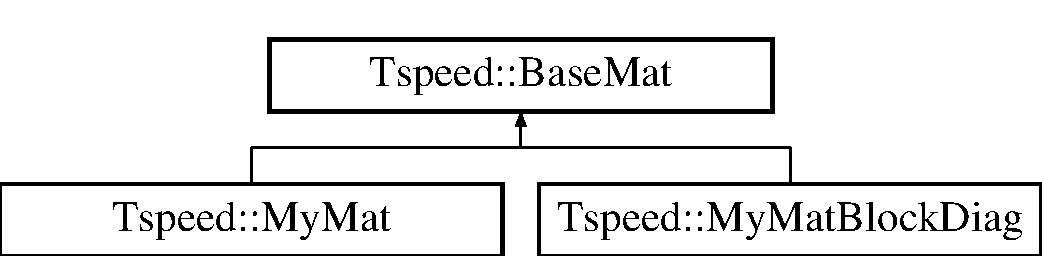
\includegraphics[height=2.000000cm]{classTspeed_1_1BaseMat}
\end{center}
\end{figure}
\subsection*{Public Member Functions}
\begin{DoxyCompactItemize}
\item 
\hyperlink{classTspeed_1_1BaseMat_a0bc33a9288577b32639974d28e686026}{Base\-Mat} ()
\item 
\hyperlink{classTspeed_1_1BaseMat_a23de2c55f78003dbadae51a3c495b9e9}{Base\-Mat} (\hyperlink{namespaceTspeed_a7367a01365c4cc2c1a09305b3effc4e8}{Mesh\-\_\-ptr}, unsigned int nln)
\item 
Eigen\-::\-Matrix\-Xd const \& \hyperlink{classTspeed_1_1BaseMat_a9abd329c5642cb0733dc9bae2bc27c40}{block} (unsigned int \hyperlink{vtk__vector__out_8m_a6f6ccfcf58b31cb6412107d9d5281426}{i}, unsigned int \hyperlink{vtk__mesh__out_8m_af1af736f0a1475ea44566768103395cb}{j}) const 
\item 
Eigen\-::\-Matrix\-Xd \& \hyperlink{classTspeed_1_1BaseMat_aee18568676b6ec413ef58292278b88b1}{block} (unsigned int \hyperlink{vtk__vector__out_8m_a6f6ccfcf58b31cb6412107d9d5281426}{i}, unsigned int \hyperlink{vtk__mesh__out_8m_af1af736f0a1475ea44566768103395cb}{j})
\item 
void \hyperlink{classTspeed_1_1BaseMat_af8995143af50b0c6296ba6565238722a}{setblock} (unsigned int \hyperlink{vtk__vector__out_8m_a6f6ccfcf58b31cb6412107d9d5281426}{i}, unsigned int \hyperlink{vtk__mesh__out_8m_af1af736f0a1475ea44566768103395cb}{j}, Eigen\-::\-Matrix\-Xd const \&M)
\item 
\hyperlink{classTspeed_1_1BaseMat_aac366647d4c8c12ffca8ab1c8fb8881a}{Base\-Mat} (\hyperlink{classTspeed_1_1BaseMat}{Base\-Mat} const \&)
\item 
virtual \hyperlink{classTspeed_1_1BaseMat_a0aa68786e0a52c9f1fe6838813a299ce}{$\sim$\-Base\-Mat} ()=default
\item 
unsigned int \hyperlink{classTspeed_1_1BaseMat_a484dafa1e629d9774c8a402945a2c132}{nr} () const 
\item 
std\-::vector$<$ unsigned int $>$ const \& \hyperlink{classTspeed_1_1BaseMat_a4340f54ae8855520777976d76a054d25}{row\-Ind} () const 
\item 
std\-::vector$<$ unsigned int $>$ const \& \hyperlink{classTspeed_1_1BaseMat_a49b084a9e5a94fd0b188c7b2fd8eb1b6}{col\-Ind} () const 
\item 
void \hyperlink{classTspeed_1_1BaseMat_ae38cb2311d29d37b11692af1bd7cbb7d}{set\-\_\-row\-Ind} (std\-::vector$<$ unsigned int $>$const \&v)
\item 
void \hyperlink{classTspeed_1_1BaseMat_ac26f40dd7c982e596214df26e4d70931}{set\-\_\-col\-Ind} (std\-::vector$<$ unsigned int $>$const \&v)
\item 
std\-::vector$<$ Eigen\-::\-Matrix\-Xd $>$\\*
 const \& \hyperlink{classTspeed_1_1BaseMat_a71819b73e763c000d5ec02546f81c16f}{elem} () const 
\item 
std\-::vector$<$ Eigen\-::\-Matrix\-Xd $>$ \& \hyperlink{classTspeed_1_1BaseMat_af29296b4ded5241e8813d40a0a032856}{elem} ()
\item 
Eigen\-::\-Matrix\-Xd const \& \hyperlink{classTspeed_1_1BaseMat_abce23dbc10f2dea5894cf72ac6daee75}{elem} (int \hyperlink{vtk__vector__out_8m_a6f6ccfcf58b31cb6412107d9d5281426}{i}) const 
\item 
unsigned int \hyperlink{classTspeed_1_1BaseMat_ad7ab902ff362d6a356fdde29ae39e9db}{size} () const 
\item 
void \hyperlink{classTspeed_1_1BaseMat_a8fdb94992f87a903132a7c1848221d4f}{vec\-Mult} (Eigen\-::\-Vector\-Xd const \&, Eigen\-::\-Vector\-Xd \&) const 
\end{DoxyCompactItemize}
\subsection*{Protected Attributes}
\begin{DoxyCompactItemize}
\item 
unsigned int \hyperlink{classTspeed_1_1BaseMat_a2122ee11f990f68aadf6046e7c02aa01}{M\-\_\-nr}
\item 
unsigned int \hyperlink{classTspeed_1_1BaseMat_aaeeb3b9b5163d2ad7213877c6d9d3a48}{M\-\_\-nc}
\item 
unsigned int \hyperlink{classTspeed_1_1BaseMat_a6a75298d3c989a182f972916f894df47}{M\-\_\-nln}
\item 
std\-::vector$<$ Eigen\-::\-Matrix\-Xd $>$ \hyperlink{classTspeed_1_1BaseMat_a4020a63099be7634e355b66c21a37bc0}{M\-\_\-m}
\item 
std\-::vector$<$ unsigned int $>$ \hyperlink{classTspeed_1_1BaseMat_a8147ef48c03cd2080c35e35c213c21aa}{M\-\_\-r}
\item 
std\-::vector$<$ unsigned int $>$ \hyperlink{classTspeed_1_1BaseMat_a0c1966f176c1bf095decc0f40fd2397f}{M\-\_\-c}
\end{DoxyCompactItemize}


\subsection{Constructor \& Destructor Documentation}
\hypertarget{classTspeed_1_1BaseMat_a0bc33a9288577b32639974d28e686026}{\index{Tspeed\-::\-Base\-Mat@{Tspeed\-::\-Base\-Mat}!Base\-Mat@{Base\-Mat}}
\index{Base\-Mat@{Base\-Mat}!Tspeed::BaseMat@{Tspeed\-::\-Base\-Mat}}
\subsubsection[{Base\-Mat}]{\setlength{\rightskip}{0pt plus 5cm}Tspeed\-::\-Base\-Mat\-::\-Base\-Mat (
\begin{DoxyParamCaption}
{}
\end{DoxyParamCaption}
)}}\label{classTspeed_1_1BaseMat_a0bc33a9288577b32639974d28e686026}
\hypertarget{classTspeed_1_1BaseMat_a23de2c55f78003dbadae51a3c495b9e9}{\index{Tspeed\-::\-Base\-Mat@{Tspeed\-::\-Base\-Mat}!Base\-Mat@{Base\-Mat}}
\index{Base\-Mat@{Base\-Mat}!Tspeed::BaseMat@{Tspeed\-::\-Base\-Mat}}
\subsubsection[{Base\-Mat}]{\setlength{\rightskip}{0pt plus 5cm}Tspeed\-::\-Base\-Mat\-::\-Base\-Mat (
\begin{DoxyParamCaption}
\item[{{\bf Mesh\-\_\-ptr}}]{, }
\item[{unsigned int}]{nln}
\end{DoxyParamCaption}
)}}\label{classTspeed_1_1BaseMat_a23de2c55f78003dbadae51a3c495b9e9}
\hypertarget{classTspeed_1_1BaseMat_aac366647d4c8c12ffca8ab1c8fb8881a}{\index{Tspeed\-::\-Base\-Mat@{Tspeed\-::\-Base\-Mat}!Base\-Mat@{Base\-Mat}}
\index{Base\-Mat@{Base\-Mat}!Tspeed::BaseMat@{Tspeed\-::\-Base\-Mat}}
\subsubsection[{Base\-Mat}]{\setlength{\rightskip}{0pt plus 5cm}Tspeed\-::\-Base\-Mat\-::\-Base\-Mat (
\begin{DoxyParamCaption}
\item[{{\bf Base\-Mat} const \&}]{}
\end{DoxyParamCaption}
)}}\label{classTspeed_1_1BaseMat_aac366647d4c8c12ffca8ab1c8fb8881a}
\hypertarget{classTspeed_1_1BaseMat_a0aa68786e0a52c9f1fe6838813a299ce}{\index{Tspeed\-::\-Base\-Mat@{Tspeed\-::\-Base\-Mat}!$\sim$\-Base\-Mat@{$\sim$\-Base\-Mat}}
\index{$\sim$\-Base\-Mat@{$\sim$\-Base\-Mat}!Tspeed::BaseMat@{Tspeed\-::\-Base\-Mat}}
\subsubsection[{$\sim$\-Base\-Mat}]{\setlength{\rightskip}{0pt plus 5cm}virtual Tspeed\-::\-Base\-Mat\-::$\sim$\-Base\-Mat (
\begin{DoxyParamCaption}
{}
\end{DoxyParamCaption}
)\hspace{0.3cm}{\ttfamily [virtual]}, {\ttfamily [default]}}}\label{classTspeed_1_1BaseMat_a0aa68786e0a52c9f1fe6838813a299ce}


\subsection{Member Function Documentation}
\hypertarget{classTspeed_1_1BaseMat_a9abd329c5642cb0733dc9bae2bc27c40}{\index{Tspeed\-::\-Base\-Mat@{Tspeed\-::\-Base\-Mat}!block@{block}}
\index{block@{block}!Tspeed::BaseMat@{Tspeed\-::\-Base\-Mat}}
\subsubsection[{block}]{\setlength{\rightskip}{0pt plus 5cm}Eigen\-::\-Matrix\-Xd const \& Tspeed\-::\-Base\-Mat\-::block (
\begin{DoxyParamCaption}
\item[{unsigned int}]{i, }
\item[{unsigned int}]{j}
\end{DoxyParamCaption}
) const}}\label{classTspeed_1_1BaseMat_a9abd329c5642cb0733dc9bae2bc27c40}
\hypertarget{classTspeed_1_1BaseMat_aee18568676b6ec413ef58292278b88b1}{\index{Tspeed\-::\-Base\-Mat@{Tspeed\-::\-Base\-Mat}!block@{block}}
\index{block@{block}!Tspeed::BaseMat@{Tspeed\-::\-Base\-Mat}}
\subsubsection[{block}]{\setlength{\rightskip}{0pt plus 5cm}Eigen\-::\-Matrix\-Xd \& Tspeed\-::\-Base\-Mat\-::block (
\begin{DoxyParamCaption}
\item[{unsigned int}]{i, }
\item[{unsigned int}]{j}
\end{DoxyParamCaption}
)}}\label{classTspeed_1_1BaseMat_aee18568676b6ec413ef58292278b88b1}
\hypertarget{classTspeed_1_1BaseMat_a49b084a9e5a94fd0b188c7b2fd8eb1b6}{\index{Tspeed\-::\-Base\-Mat@{Tspeed\-::\-Base\-Mat}!col\-Ind@{col\-Ind}}
\index{col\-Ind@{col\-Ind}!Tspeed::BaseMat@{Tspeed\-::\-Base\-Mat}}
\subsubsection[{col\-Ind}]{\setlength{\rightskip}{0pt plus 5cm}std\-::vector$<$unsigned int$>$ const\& Tspeed\-::\-Base\-Mat\-::col\-Ind (
\begin{DoxyParamCaption}
{}
\end{DoxyParamCaption}
) const\hspace{0.3cm}{\ttfamily [inline]}}}\label{classTspeed_1_1BaseMat_a49b084a9e5a94fd0b188c7b2fd8eb1b6}
\hypertarget{classTspeed_1_1BaseMat_a71819b73e763c000d5ec02546f81c16f}{\index{Tspeed\-::\-Base\-Mat@{Tspeed\-::\-Base\-Mat}!elem@{elem}}
\index{elem@{elem}!Tspeed::BaseMat@{Tspeed\-::\-Base\-Mat}}
\subsubsection[{elem}]{\setlength{\rightskip}{0pt plus 5cm}std\-::vector$<$Eigen\-::\-Matrix\-Xd$>$ const\& Tspeed\-::\-Base\-Mat\-::elem (
\begin{DoxyParamCaption}
{}
\end{DoxyParamCaption}
) const\hspace{0.3cm}{\ttfamily [inline]}}}\label{classTspeed_1_1BaseMat_a71819b73e763c000d5ec02546f81c16f}
\hypertarget{classTspeed_1_1BaseMat_af29296b4ded5241e8813d40a0a032856}{\index{Tspeed\-::\-Base\-Mat@{Tspeed\-::\-Base\-Mat}!elem@{elem}}
\index{elem@{elem}!Tspeed::BaseMat@{Tspeed\-::\-Base\-Mat}}
\subsubsection[{elem}]{\setlength{\rightskip}{0pt plus 5cm}std\-::vector$<$Eigen\-::\-Matrix\-Xd$>$\& Tspeed\-::\-Base\-Mat\-::elem (
\begin{DoxyParamCaption}
{}
\end{DoxyParamCaption}
)\hspace{0.3cm}{\ttfamily [inline]}}}\label{classTspeed_1_1BaseMat_af29296b4ded5241e8813d40a0a032856}
\hypertarget{classTspeed_1_1BaseMat_abce23dbc10f2dea5894cf72ac6daee75}{\index{Tspeed\-::\-Base\-Mat@{Tspeed\-::\-Base\-Mat}!elem@{elem}}
\index{elem@{elem}!Tspeed::BaseMat@{Tspeed\-::\-Base\-Mat}}
\subsubsection[{elem}]{\setlength{\rightskip}{0pt plus 5cm}Eigen\-::\-Matrix\-Xd const\& Tspeed\-::\-Base\-Mat\-::elem (
\begin{DoxyParamCaption}
\item[{int}]{i}
\end{DoxyParamCaption}
) const\hspace{0.3cm}{\ttfamily [inline]}}}\label{classTspeed_1_1BaseMat_abce23dbc10f2dea5894cf72ac6daee75}
\hypertarget{classTspeed_1_1BaseMat_a484dafa1e629d9774c8a402945a2c132}{\index{Tspeed\-::\-Base\-Mat@{Tspeed\-::\-Base\-Mat}!nr@{nr}}
\index{nr@{nr}!Tspeed::BaseMat@{Tspeed\-::\-Base\-Mat}}
\subsubsection[{nr}]{\setlength{\rightskip}{0pt plus 5cm}unsigned int Tspeed\-::\-Base\-Mat\-::nr (
\begin{DoxyParamCaption}
{}
\end{DoxyParamCaption}
) const\hspace{0.3cm}{\ttfamily [inline]}}}\label{classTspeed_1_1BaseMat_a484dafa1e629d9774c8a402945a2c132}
\hypertarget{classTspeed_1_1BaseMat_a4340f54ae8855520777976d76a054d25}{\index{Tspeed\-::\-Base\-Mat@{Tspeed\-::\-Base\-Mat}!row\-Ind@{row\-Ind}}
\index{row\-Ind@{row\-Ind}!Tspeed::BaseMat@{Tspeed\-::\-Base\-Mat}}
\subsubsection[{row\-Ind}]{\setlength{\rightskip}{0pt plus 5cm}std\-::vector$<$unsigned int$>$ const\& Tspeed\-::\-Base\-Mat\-::row\-Ind (
\begin{DoxyParamCaption}
{}
\end{DoxyParamCaption}
) const\hspace{0.3cm}{\ttfamily [inline]}}}\label{classTspeed_1_1BaseMat_a4340f54ae8855520777976d76a054d25}
\hypertarget{classTspeed_1_1BaseMat_ac26f40dd7c982e596214df26e4d70931}{\index{Tspeed\-::\-Base\-Mat@{Tspeed\-::\-Base\-Mat}!set\-\_\-col\-Ind@{set\-\_\-col\-Ind}}
\index{set\-\_\-col\-Ind@{set\-\_\-col\-Ind}!Tspeed::BaseMat@{Tspeed\-::\-Base\-Mat}}
\subsubsection[{set\-\_\-col\-Ind}]{\setlength{\rightskip}{0pt plus 5cm}void Tspeed\-::\-Base\-Mat\-::set\-\_\-col\-Ind (
\begin{DoxyParamCaption}
\item[{std\-::vector$<$ unsigned int $>$const \&}]{v}
\end{DoxyParamCaption}
)\hspace{0.3cm}{\ttfamily [inline]}}}\label{classTspeed_1_1BaseMat_ac26f40dd7c982e596214df26e4d70931}
\hypertarget{classTspeed_1_1BaseMat_ae38cb2311d29d37b11692af1bd7cbb7d}{\index{Tspeed\-::\-Base\-Mat@{Tspeed\-::\-Base\-Mat}!set\-\_\-row\-Ind@{set\-\_\-row\-Ind}}
\index{set\-\_\-row\-Ind@{set\-\_\-row\-Ind}!Tspeed::BaseMat@{Tspeed\-::\-Base\-Mat}}
\subsubsection[{set\-\_\-row\-Ind}]{\setlength{\rightskip}{0pt plus 5cm}void Tspeed\-::\-Base\-Mat\-::set\-\_\-row\-Ind (
\begin{DoxyParamCaption}
\item[{std\-::vector$<$ unsigned int $>$const \&}]{v}
\end{DoxyParamCaption}
)\hspace{0.3cm}{\ttfamily [inline]}}}\label{classTspeed_1_1BaseMat_ae38cb2311d29d37b11692af1bd7cbb7d}
\hypertarget{classTspeed_1_1BaseMat_af8995143af50b0c6296ba6565238722a}{\index{Tspeed\-::\-Base\-Mat@{Tspeed\-::\-Base\-Mat}!setblock@{setblock}}
\index{setblock@{setblock}!Tspeed::BaseMat@{Tspeed\-::\-Base\-Mat}}
\subsubsection[{setblock}]{\setlength{\rightskip}{0pt plus 5cm}void Tspeed\-::\-Base\-Mat\-::setblock (
\begin{DoxyParamCaption}
\item[{unsigned int}]{i, }
\item[{unsigned int}]{j, }
\item[{Eigen\-::\-Matrix\-Xd const \&}]{M}
\end{DoxyParamCaption}
)}}\label{classTspeed_1_1BaseMat_af8995143af50b0c6296ba6565238722a}
\hypertarget{classTspeed_1_1BaseMat_ad7ab902ff362d6a356fdde29ae39e9db}{\index{Tspeed\-::\-Base\-Mat@{Tspeed\-::\-Base\-Mat}!size@{size}}
\index{size@{size}!Tspeed::BaseMat@{Tspeed\-::\-Base\-Mat}}
\subsubsection[{size}]{\setlength{\rightskip}{0pt plus 5cm}unsigned int Tspeed\-::\-Base\-Mat\-::size (
\begin{DoxyParamCaption}
{}
\end{DoxyParamCaption}
) const\hspace{0.3cm}{\ttfamily [inline]}}}\label{classTspeed_1_1BaseMat_ad7ab902ff362d6a356fdde29ae39e9db}
\hypertarget{classTspeed_1_1BaseMat_a8fdb94992f87a903132a7c1848221d4f}{\index{Tspeed\-::\-Base\-Mat@{Tspeed\-::\-Base\-Mat}!vec\-Mult@{vec\-Mult}}
\index{vec\-Mult@{vec\-Mult}!Tspeed::BaseMat@{Tspeed\-::\-Base\-Mat}}
\subsubsection[{vec\-Mult}]{\setlength{\rightskip}{0pt plus 5cm}void Tspeed\-::\-Base\-Mat\-::vec\-Mult (
\begin{DoxyParamCaption}
\item[{Eigen\-::\-Vector\-Xd const \&}]{x, }
\item[{Eigen\-::\-Vector\-Xd \&}]{out}
\end{DoxyParamCaption}
) const}}\label{classTspeed_1_1BaseMat_a8fdb94992f87a903132a7c1848221d4f}


\subsection{Member Data Documentation}
\hypertarget{classTspeed_1_1BaseMat_a0c1966f176c1bf095decc0f40fd2397f}{\index{Tspeed\-::\-Base\-Mat@{Tspeed\-::\-Base\-Mat}!M\-\_\-c@{M\-\_\-c}}
\index{M\-\_\-c@{M\-\_\-c}!Tspeed::BaseMat@{Tspeed\-::\-Base\-Mat}}
\subsubsection[{M\-\_\-c}]{\setlength{\rightskip}{0pt plus 5cm}std\-::vector$<$unsigned int$>$ Tspeed\-::\-Base\-Mat\-::\-M\-\_\-c\hspace{0.3cm}{\ttfamily [protected]}}}\label{classTspeed_1_1BaseMat_a0c1966f176c1bf095decc0f40fd2397f}
\hypertarget{classTspeed_1_1BaseMat_a4020a63099be7634e355b66c21a37bc0}{\index{Tspeed\-::\-Base\-Mat@{Tspeed\-::\-Base\-Mat}!M\-\_\-m@{M\-\_\-m}}
\index{M\-\_\-m@{M\-\_\-m}!Tspeed::BaseMat@{Tspeed\-::\-Base\-Mat}}
\subsubsection[{M\-\_\-m}]{\setlength{\rightskip}{0pt plus 5cm}std\-::vector$<$Eigen\-::\-Matrix\-Xd$>$ Tspeed\-::\-Base\-Mat\-::\-M\-\_\-m\hspace{0.3cm}{\ttfamily [protected]}}}\label{classTspeed_1_1BaseMat_a4020a63099be7634e355b66c21a37bc0}
\hypertarget{classTspeed_1_1BaseMat_aaeeb3b9b5163d2ad7213877c6d9d3a48}{\index{Tspeed\-::\-Base\-Mat@{Tspeed\-::\-Base\-Mat}!M\-\_\-nc@{M\-\_\-nc}}
\index{M\-\_\-nc@{M\-\_\-nc}!Tspeed::BaseMat@{Tspeed\-::\-Base\-Mat}}
\subsubsection[{M\-\_\-nc}]{\setlength{\rightskip}{0pt plus 5cm}unsigned int Tspeed\-::\-Base\-Mat\-::\-M\-\_\-nc\hspace{0.3cm}{\ttfamily [protected]}}}\label{classTspeed_1_1BaseMat_aaeeb3b9b5163d2ad7213877c6d9d3a48}
\hypertarget{classTspeed_1_1BaseMat_a6a75298d3c989a182f972916f894df47}{\index{Tspeed\-::\-Base\-Mat@{Tspeed\-::\-Base\-Mat}!M\-\_\-nln@{M\-\_\-nln}}
\index{M\-\_\-nln@{M\-\_\-nln}!Tspeed::BaseMat@{Tspeed\-::\-Base\-Mat}}
\subsubsection[{M\-\_\-nln}]{\setlength{\rightskip}{0pt plus 5cm}unsigned int Tspeed\-::\-Base\-Mat\-::\-M\-\_\-nln\hspace{0.3cm}{\ttfamily [protected]}}}\label{classTspeed_1_1BaseMat_a6a75298d3c989a182f972916f894df47}
\hypertarget{classTspeed_1_1BaseMat_a2122ee11f990f68aadf6046e7c02aa01}{\index{Tspeed\-::\-Base\-Mat@{Tspeed\-::\-Base\-Mat}!M\-\_\-nr@{M\-\_\-nr}}
\index{M\-\_\-nr@{M\-\_\-nr}!Tspeed::BaseMat@{Tspeed\-::\-Base\-Mat}}
\subsubsection[{M\-\_\-nr}]{\setlength{\rightskip}{0pt plus 5cm}unsigned int Tspeed\-::\-Base\-Mat\-::\-M\-\_\-nr\hspace{0.3cm}{\ttfamily [protected]}}}\label{classTspeed_1_1BaseMat_a2122ee11f990f68aadf6046e7c02aa01}
\hypertarget{classTspeed_1_1BaseMat_a8147ef48c03cd2080c35e35c213c21aa}{\index{Tspeed\-::\-Base\-Mat@{Tspeed\-::\-Base\-Mat}!M\-\_\-r@{M\-\_\-r}}
\index{M\-\_\-r@{M\-\_\-r}!Tspeed::BaseMat@{Tspeed\-::\-Base\-Mat}}
\subsubsection[{M\-\_\-r}]{\setlength{\rightskip}{0pt plus 5cm}std\-::vector$<$unsigned int$>$ Tspeed\-::\-Base\-Mat\-::\-M\-\_\-r\hspace{0.3cm}{\ttfamily [protected]}}}\label{classTspeed_1_1BaseMat_a8147ef48c03cd2080c35e35c213c21aa}


The documentation for this class was generated from the following files\-:\begin{DoxyCompactItemize}
\item 
lib/include/\hyperlink{MyMat_8hpp}{My\-Mat.\-hpp}\item 
lib/src/\hyperlink{MyMat_8cpp}{My\-Mat.\-cpp}\end{DoxyCompactItemize}

\hypertarget{classTspeed_1_1BoundaryAdapted}{\section{Tspeed\-:\-:Boundary\-Adapted$<$ N $>$ Class Template Reference}
\label{classTspeed_1_1BoundaryAdapted}\index{Tspeed\-::\-Boundary\-Adapted$<$ N $>$@{Tspeed\-::\-Boundary\-Adapted$<$ N $>$}}
}


Boundary adapted \mbox{[}2\mbox{]} basis.  




{\ttfamily \#include $<$Shape\-Functions.\-hpp$>$}

Inheritance diagram for Tspeed\-:\-:Boundary\-Adapted$<$ N $>$\-:\begin{figure}[H]
\begin{center}
\leavevmode
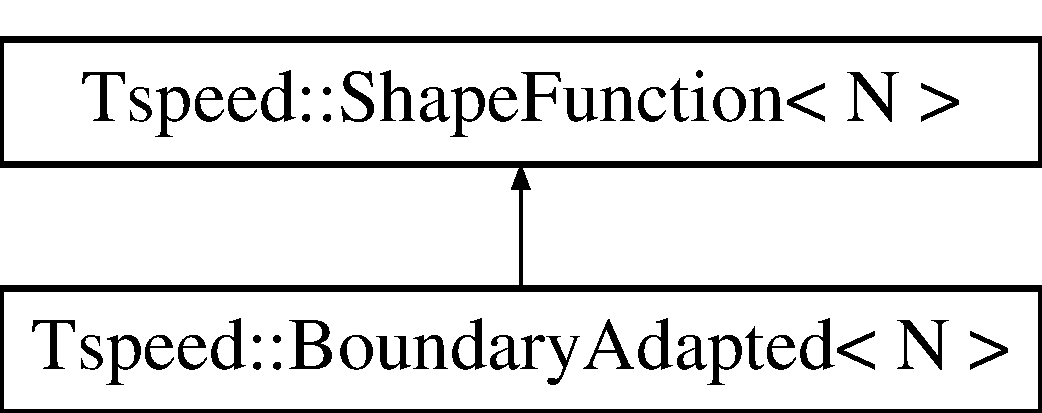
\includegraphics[height=2.000000cm]{classTspeed_1_1BoundaryAdapted}
\end{center}
\end{figure}
\subsection*{Public Types}
\begin{DoxyCompactItemize}
\item 
enum \{ \hyperlink{classTspeed_1_1BoundaryAdapted_a43bbb02cefcd3061b7b85ee061d0fe21a14fd943d0e78f08196b5f0f9e05232ce}{is\-\_\-orthonormal} = false
 \}
\begin{DoxyCompactList}\small\item\em The basis is not orthonormal. \end{DoxyCompactList}\end{DoxyCompactItemize}
\subsection*{Public Member Functions}
\begin{DoxyCompactItemize}
\item 
virtual \hyperlink{classTspeed_1_1BoundaryAdapted_a0a85bcdf3da9c2a7db73f485fb83aa3f}{$\sim$\-Boundary\-Adapted} ()
\item 
\hyperlink{classTspeed_1_1BoundaryAdapted_a9e2a2066ba91ed177411d9ab0290e706}{Boundary\-Adapted} ()
\end{DoxyCompactItemize}
\subsection*{Additional Inherited Members}


\subsection{Detailed Description}
\subsubsection*{template$<$int N$>$class Tspeed\-::\-Boundary\-Adapted$<$ N $>$}

Boundary adapted \mbox{[}2\mbox{]} basis. 


\begin{DoxyTemplParams}{Template Parameters}
{\em N} & degree of the space $\mathbb{N}$ \\
\hline
\end{DoxyTemplParams}


\subsection{Member Enumeration Documentation}
\hypertarget{classTspeed_1_1BoundaryAdapted_a43bbb02cefcd3061b7b85ee061d0fe21}{\subsubsection[{anonymous enum}]{\setlength{\rightskip}{0pt plus 5cm}template$<$int N$>$ anonymous enum}}\label{classTspeed_1_1BoundaryAdapted_a43bbb02cefcd3061b7b85ee061d0fe21}


The basis is not orthonormal. 

\begin{Desc}
\item[Enumerator]\par
\begin{description}
\index{is\-\_\-orthonormal@{is\-\_\-orthonormal}!Tspeed\-::\-Boundary\-Adapted@{Tspeed\-::\-Boundary\-Adapted}}\index{Tspeed\-::\-Boundary\-Adapted@{Tspeed\-::\-Boundary\-Adapted}!is\-\_\-orthonormal@{is\-\_\-orthonormal}}\item[{\em 
\hypertarget{classTspeed_1_1BoundaryAdapted_a43bbb02cefcd3061b7b85ee061d0fe21a14fd943d0e78f08196b5f0f9e05232ce}{is\-\_\-orthonormal}\label{classTspeed_1_1BoundaryAdapted_a43bbb02cefcd3061b7b85ee061d0fe21a14fd943d0e78f08196b5f0f9e05232ce}
}]\end{description}
\end{Desc}


\subsection{Constructor \& Destructor Documentation}
\hypertarget{classTspeed_1_1BoundaryAdapted_a0a85bcdf3da9c2a7db73f485fb83aa3f}{\index{Tspeed\-::\-Boundary\-Adapted@{Tspeed\-::\-Boundary\-Adapted}!$\sim$\-Boundary\-Adapted@{$\sim$\-Boundary\-Adapted}}
\index{$\sim$\-Boundary\-Adapted@{$\sim$\-Boundary\-Adapted}!Tspeed::BoundaryAdapted@{Tspeed\-::\-Boundary\-Adapted}}
\subsubsection[{$\sim$\-Boundary\-Adapted}]{\setlength{\rightskip}{0pt plus 5cm}template$<$int N$>$ virtual {\bf Tspeed\-::\-Boundary\-Adapted}$<$ N $>$\-::$\sim${\bf Boundary\-Adapted} (
\begin{DoxyParamCaption}
{}
\end{DoxyParamCaption}
)\hspace{0.3cm}{\ttfamily [inline]}, {\ttfamily [virtual]}}}\label{classTspeed_1_1BoundaryAdapted_a0a85bcdf3da9c2a7db73f485fb83aa3f}
\hypertarget{classTspeed_1_1BoundaryAdapted_a9e2a2066ba91ed177411d9ab0290e706}{\index{Tspeed\-::\-Boundary\-Adapted@{Tspeed\-::\-Boundary\-Adapted}!Boundary\-Adapted@{Boundary\-Adapted}}
\index{Boundary\-Adapted@{Boundary\-Adapted}!Tspeed::BoundaryAdapted@{Tspeed\-::\-Boundary\-Adapted}}
\subsubsection[{Boundary\-Adapted}]{\setlength{\rightskip}{0pt plus 5cm}template$<$int N$>$ {\bf Tspeed\-::\-Boundary\-Adapted}$<$ N $>$\-::{\bf Boundary\-Adapted} (
\begin{DoxyParamCaption}
{}
\end{DoxyParamCaption}
)}}\label{classTspeed_1_1BoundaryAdapted_a9e2a2066ba91ed177411d9ab0290e706}


The documentation for this class was generated from the following files\-:\begin{DoxyCompactItemize}
\item 
lib/include/\hyperlink{ShapeFunctions_8hpp}{Shape\-Functions.\-hpp}\item 
lib/include/\hyperlink{ShapeFunctions__imp_8hpp}{Shape\-Functions\-\_\-imp.\-hpp}\end{DoxyCompactItemize}

\hypertarget{classTspeed_1_1Dubiner}{\section{Tspeed\-:\-:Dubiner$<$ N $>$ Class Template Reference}
\label{classTspeed_1_1Dubiner}\index{Tspeed\-::\-Dubiner$<$ N $>$@{Tspeed\-::\-Dubiner$<$ N $>$}}
}


\hyperlink{classTspeed_1_1Dubiner}{Dubiner} \mbox{[}1\mbox{]} basis.  




{\ttfamily \#include $<$Shape\-Functions.\-hpp$>$}

Inheritance diagram for Tspeed\-:\-:Dubiner$<$ N $>$\-:\begin{figure}[H]
\begin{center}
\leavevmode
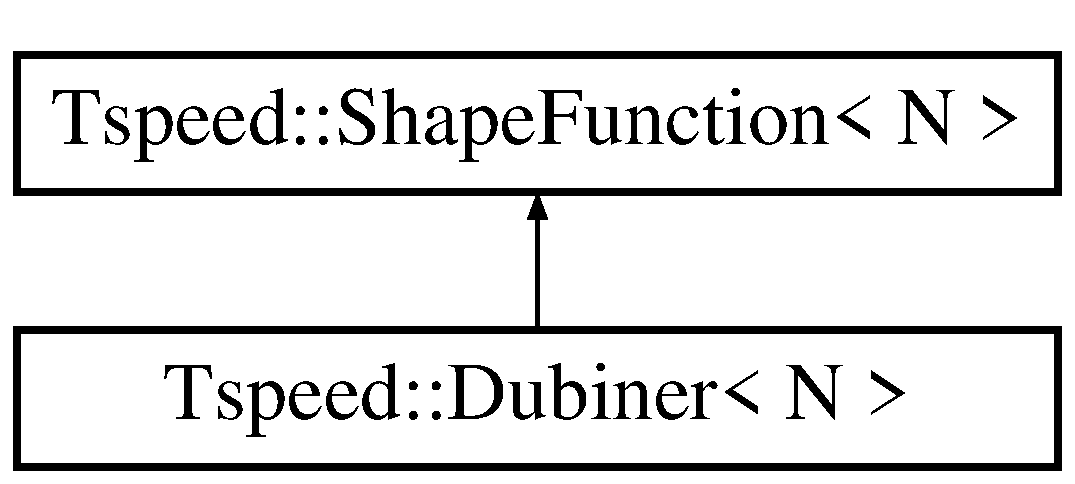
\includegraphics[height=2.000000cm]{classTspeed_1_1Dubiner}
\end{center}
\end{figure}
\subsection*{Public Types}
\begin{DoxyCompactItemize}
\item 
enum \{ \hyperlink{classTspeed_1_1Dubiner_aee2eaa9dbcd2aa93d7d951a9c61a10e2a749d33573b6e1a4f9c56e9d5322fd70c}{is\-\_\-orthonormal} = true
 \}
\begin{DoxyCompactList}\small\item\em \hyperlink{classTspeed_1_1Dubiner}{Dubiner} basis is orthonormal. \end{DoxyCompactList}\end{DoxyCompactItemize}
\subsection*{Public Member Functions}
\begin{DoxyCompactItemize}
\item 
virtual \hyperlink{classTspeed_1_1Dubiner_a3739d778c878f28ad63a062a210a69ae}{$\sim$\-Dubiner} ()
\item 
\hyperlink{classTspeed_1_1Dubiner_a0a4315462e09a1d2e4695b3f636ccd35}{Dubiner} ()
\end{DoxyCompactItemize}
\subsection*{Additional Inherited Members}


\subsection{Detailed Description}
\subsubsection*{template$<$int N$>$class Tspeed\-::\-Dubiner$<$ N $>$}

\hyperlink{classTspeed_1_1Dubiner}{Dubiner} \mbox{[}1\mbox{]} basis. 


\begin{DoxyTemplParams}{Template Parameters}
{\em N} & degree of the space $\mathbb{N}$ \\
\hline
\end{DoxyTemplParams}


\subsection{Member Enumeration Documentation}
\hypertarget{classTspeed_1_1Dubiner_aee2eaa9dbcd2aa93d7d951a9c61a10e2}{\subsubsection[{anonymous enum}]{\setlength{\rightskip}{0pt plus 5cm}template$<$int N$>$ anonymous enum}}\label{classTspeed_1_1Dubiner_aee2eaa9dbcd2aa93d7d951a9c61a10e2}


\hyperlink{classTspeed_1_1Dubiner}{Dubiner} basis is orthonormal. 

\begin{Desc}
\item[Enumerator]\par
\begin{description}
\index{is\-\_\-orthonormal@{is\-\_\-orthonormal}!Tspeed\-::\-Dubiner@{Tspeed\-::\-Dubiner}}\index{Tspeed\-::\-Dubiner@{Tspeed\-::\-Dubiner}!is\-\_\-orthonormal@{is\-\_\-orthonormal}}\item[{\em 
\hypertarget{classTspeed_1_1Dubiner_aee2eaa9dbcd2aa93d7d951a9c61a10e2a749d33573b6e1a4f9c56e9d5322fd70c}{is\-\_\-orthonormal}\label{classTspeed_1_1Dubiner_aee2eaa9dbcd2aa93d7d951a9c61a10e2a749d33573b6e1a4f9c56e9d5322fd70c}
}]\end{description}
\end{Desc}


\subsection{Constructor \& Destructor Documentation}
\hypertarget{classTspeed_1_1Dubiner_a3739d778c878f28ad63a062a210a69ae}{\index{Tspeed\-::\-Dubiner@{Tspeed\-::\-Dubiner}!$\sim$\-Dubiner@{$\sim$\-Dubiner}}
\index{$\sim$\-Dubiner@{$\sim$\-Dubiner}!Tspeed::Dubiner@{Tspeed\-::\-Dubiner}}
\subsubsection[{$\sim$\-Dubiner}]{\setlength{\rightskip}{0pt plus 5cm}template$<$int N$>$ virtual {\bf Tspeed\-::\-Dubiner}$<$ N $>$\-::$\sim${\bf Dubiner} (
\begin{DoxyParamCaption}
{}
\end{DoxyParamCaption}
)\hspace{0.3cm}{\ttfamily [inline]}, {\ttfamily [virtual]}}}\label{classTspeed_1_1Dubiner_a3739d778c878f28ad63a062a210a69ae}
\hypertarget{classTspeed_1_1Dubiner_a0a4315462e09a1d2e4695b3f636ccd35}{\index{Tspeed\-::\-Dubiner@{Tspeed\-::\-Dubiner}!Dubiner@{Dubiner}}
\index{Dubiner@{Dubiner}!Tspeed::Dubiner@{Tspeed\-::\-Dubiner}}
\subsubsection[{Dubiner}]{\setlength{\rightskip}{0pt plus 5cm}template$<$int N$>$ {\bf Tspeed\-::\-Dubiner}$<$ N $>$\-::{\bf Dubiner} (
\begin{DoxyParamCaption}
{}
\end{DoxyParamCaption}
)}}\label{classTspeed_1_1Dubiner_a0a4315462e09a1d2e4695b3f636ccd35}


The documentation for this class was generated from the following files\-:\begin{DoxyCompactItemize}
\item 
lib/include/\hyperlink{ShapeFunctions_8hpp}{Shape\-Functions.\-hpp}\item 
lib/include/\hyperlink{ShapeFunctions__imp_8hpp}{Shape\-Functions\-\_\-imp.\-hpp}\end{DoxyCompactItemize}

\hypertarget{classTspeed_1_1Dunavant}{\section{Tspeed\-:\-:Dunavant$<$ N $>$ Class Template Reference}
\label{classTspeed_1_1Dunavant}\index{Tspeed\-::\-Dunavant$<$ N $>$@{Tspeed\-::\-Dunavant$<$ N $>$}}
}


\hyperlink{classTspeed_1_1Dunavant}{Dunavant} \mbox{[}1\mbox{]} quadrature rule.  




{\ttfamily \#include $<$Quadrature\-Rule.\-hpp$>$}

Inheritance diagram for Tspeed\-:\-:Dunavant$<$ N $>$\-:\begin{figure}[H]
\begin{center}
\leavevmode
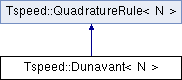
\includegraphics[height=2.000000cm]{classTspeed_1_1Dunavant}
\end{center}
\end{figure}
\subsection*{Public Types}
\begin{DoxyCompactItemize}
\item 
enum \{ \hyperlink{classTspeed_1_1Dunavant_a5490f3fa01eb0b3072ee657afc64053fa9142a1285dd27e2e329bf53154974324}{nqn2d} = dunavant\-\_\-num\-\_\-points$<$N$>$()
 \}
\item 
enum \{ \hyperlink{classTspeed_1_1Dunavant_a69286a2b90f14407f1133581a2667919a3ba00ee4f1fc556134ca24ff435e53eb}{nqn1d} = N
 \}
\item 
typedef \hyperlink{classTspeed_1_1QuadratureRule}{Quadrature\-Rule}$<$ N $>$\-::\hyperlink{classTspeed_1_1QuadratureRule_a195c2b71ad957c9dc5408452b11e1302}{Vec} \hyperlink{classTspeed_1_1Dunavant_a8562daa3d038126144415fa4ba851e81}{Vec}
\item 
typedef \hyperlink{classTspeed_1_1QuadratureRule}{Quadrature\-Rule}$<$ N $>$\-::\hyperlink{classTspeed_1_1QuadratureRule_a195c2b71ad957c9dc5408452b11e1302}{Vec} \hyperlink{classTspeed_1_1Dunavant_a87e65aed6cfa6ace8ea6374f3b005d78}{Mat}
\item 
typedef \hyperlink{classTspeed_1_1QuadratureRule}{Quadrature\-Rule}$<$ N $>$\-::\hyperlink{classTspeed_1_1QuadratureRule_a195c2b71ad957c9dc5408452b11e1302}{Vec} \hyperlink{classTspeed_1_1Dunavant_acc838f609850fd31cbbeb87578b1a8c5}{Vec2}
\end{DoxyCompactItemize}
\subsection*{Public Member Functions}
\begin{DoxyCompactItemize}
\item 
\hyperlink{classTspeed_1_1Dunavant_ac20f5d5f0ed9496a7b37a7ee082f635d}{Dunavant} ()
\end{DoxyCompactItemize}
\subsection*{Additional Inherited Members}


\subsection{Detailed Description}
\subsubsection*{template$<$int N$>$class Tspeed\-::\-Dunavant$<$ N $>$}

\hyperlink{classTspeed_1_1Dunavant}{Dunavant} \mbox{[}1\mbox{]} quadrature rule. 


\begin{DoxyTemplParams}{Template Parameters}
{\em N} & the order of the rule.\\
\hline
\end{DoxyTemplParams}
A rule of order N integrates exactly polynomials of order N 

\subsection{Member Typedef Documentation}
\hypertarget{classTspeed_1_1Dunavant_a87e65aed6cfa6ace8ea6374f3b005d78}{\index{Tspeed\-::\-Dunavant@{Tspeed\-::\-Dunavant}!Mat@{Mat}}
\index{Mat@{Mat}!Tspeed::Dunavant@{Tspeed\-::\-Dunavant}}
\subsubsection[{Mat}]{\setlength{\rightskip}{0pt plus 5cm}template$<$int N$>$ typedef {\bf Quadrature\-Rule}$<$N$>$\-::{\bf Vec} {\bf Tspeed\-::\-Dunavant}$<$ N $>$\-::{\bf Mat}}}\label{classTspeed_1_1Dunavant_a87e65aed6cfa6ace8ea6374f3b005d78}
\hypertarget{classTspeed_1_1Dunavant_a8562daa3d038126144415fa4ba851e81}{\index{Tspeed\-::\-Dunavant@{Tspeed\-::\-Dunavant}!Vec@{Vec}}
\index{Vec@{Vec}!Tspeed::Dunavant@{Tspeed\-::\-Dunavant}}
\subsubsection[{Vec}]{\setlength{\rightskip}{0pt plus 5cm}template$<$int N$>$ typedef {\bf Quadrature\-Rule}$<$N$>$\-::{\bf Vec} {\bf Tspeed\-::\-Dunavant}$<$ N $>$\-::{\bf Vec}}}\label{classTspeed_1_1Dunavant_a8562daa3d038126144415fa4ba851e81}
\hypertarget{classTspeed_1_1Dunavant_acc838f609850fd31cbbeb87578b1a8c5}{\index{Tspeed\-::\-Dunavant@{Tspeed\-::\-Dunavant}!Vec2@{Vec2}}
\index{Vec2@{Vec2}!Tspeed::Dunavant@{Tspeed\-::\-Dunavant}}
\subsubsection[{Vec2}]{\setlength{\rightskip}{0pt plus 5cm}template$<$int N$>$ typedef {\bf Quadrature\-Rule}$<$N$>$\-::{\bf Vec} {\bf Tspeed\-::\-Dunavant}$<$ N $>$\-::{\bf Vec2}}}\label{classTspeed_1_1Dunavant_acc838f609850fd31cbbeb87578b1a8c5}


\subsection{Member Enumeration Documentation}
\hypertarget{classTspeed_1_1Dunavant_a5490f3fa01eb0b3072ee657afc64053f}{\subsubsection[{anonymous enum}]{\setlength{\rightskip}{0pt plus 5cm}template$<$int N$>$ anonymous enum}}\label{classTspeed_1_1Dunavant_a5490f3fa01eb0b3072ee657afc64053f}
\begin{Desc}
\item[Enumerator]\par
\begin{description}
\index{nqn2d@{nqn2d}!Tspeed\-::\-Dunavant@{Tspeed\-::\-Dunavant}}\index{Tspeed\-::\-Dunavant@{Tspeed\-::\-Dunavant}!nqn2d@{nqn2d}}\item[{\em 
\hypertarget{classTspeed_1_1Dunavant_a5490f3fa01eb0b3072ee657afc64053fa9142a1285dd27e2e329bf53154974324}{nqn2d}\label{classTspeed_1_1Dunavant_a5490f3fa01eb0b3072ee657afc64053fa9142a1285dd27e2e329bf53154974324}
}]\end{description}
\end{Desc}
\hypertarget{classTspeed_1_1Dunavant_a69286a2b90f14407f1133581a2667919}{\subsubsection[{anonymous enum}]{\setlength{\rightskip}{0pt plus 5cm}template$<$int N$>$ anonymous enum}}\label{classTspeed_1_1Dunavant_a69286a2b90f14407f1133581a2667919}
\begin{Desc}
\item[Enumerator]\par
\begin{description}
\index{nqn1d@{nqn1d}!Tspeed\-::\-Dunavant@{Tspeed\-::\-Dunavant}}\index{Tspeed\-::\-Dunavant@{Tspeed\-::\-Dunavant}!nqn1d@{nqn1d}}\item[{\em 
\hypertarget{classTspeed_1_1Dunavant_a69286a2b90f14407f1133581a2667919a3ba00ee4f1fc556134ca24ff435e53eb}{nqn1d}\label{classTspeed_1_1Dunavant_a69286a2b90f14407f1133581a2667919a3ba00ee4f1fc556134ca24ff435e53eb}
}]\end{description}
\end{Desc}


\subsection{Constructor \& Destructor Documentation}
\hypertarget{classTspeed_1_1Dunavant_ac20f5d5f0ed9496a7b37a7ee082f635d}{\index{Tspeed\-::\-Dunavant@{Tspeed\-::\-Dunavant}!Dunavant@{Dunavant}}
\index{Dunavant@{Dunavant}!Tspeed::Dunavant@{Tspeed\-::\-Dunavant}}
\subsubsection[{Dunavant}]{\setlength{\rightskip}{0pt plus 5cm}template$<$int N$>$ {\bf Tspeed\-::\-Dunavant}$<$ N $>$\-::{\bf Dunavant} (
\begin{DoxyParamCaption}
{}
\end{DoxyParamCaption}
)}}\label{classTspeed_1_1Dunavant_ac20f5d5f0ed9496a7b37a7ee082f635d}


The documentation for this class was generated from the following files\-:\begin{DoxyCompactItemize}
\item 
lib/include/\hyperlink{QuadratureRule_8hpp}{Quadrature\-Rule.\-hpp}\item 
lib/include/\hyperlink{QuadratureRule__imp_8hpp}{Quadrature\-Rule\-\_\-imp.\-hpp}\end{DoxyCompactItemize}

\hypertarget{classTspeed_1_1Geo_1_1Edge}{\section{Tspeed\-:\-:Geo\-:\-:Edge Class Reference}
\label{classTspeed_1_1Geo_1_1Edge}\index{Tspeed\-::\-Geo\-::\-Edge@{Tspeed\-::\-Geo\-::\-Edge}}
}


Class describing an edge.  




{\ttfamily \#include $<$Geometry.\-hpp$>$}

Inheritance diagram for Tspeed\-:\-:Geo\-:\-:Edge\-:\begin{figure}[H]
\begin{center}
\leavevmode
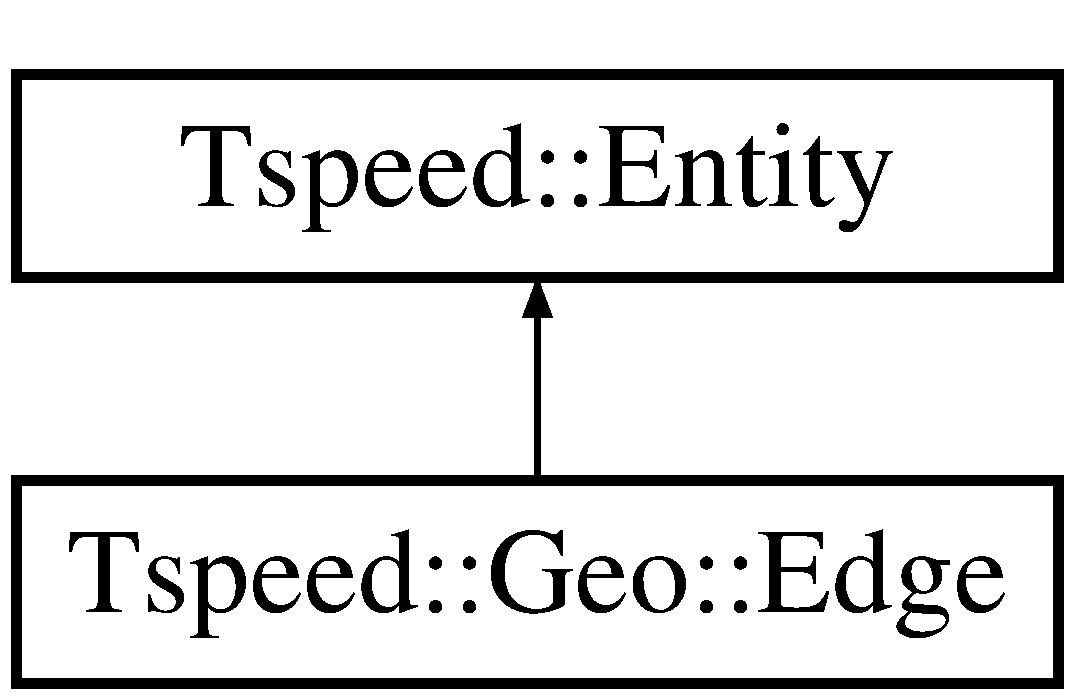
\includegraphics[height=2.000000cm]{classTspeed_1_1Geo_1_1Edge}
\end{center}
\end{figure}
\subsection*{Public Member Functions}
\begin{DoxyCompactItemize}
\item 
\hyperlink{classTspeed_1_1Geo_1_1Edge_aa28485aab77e5643067380c86c35e6b5}{Edge} ()
\begin{DoxyCompactList}\small\item\em Default constructor\-: extremal points are initialized to 0. \end{DoxyCompactList}\item 
\hyperlink{classTspeed_1_1Geo_1_1Edge_aa0c751bf90737874583ef5dbf901f669}{Edge} (const \hyperlink{classTspeed_1_1Geo_1_1Point}{Point} \&a, const \hyperlink{classTspeed_1_1Geo_1_1Point}{Point} \&b)
\begin{DoxyCompactList}\small\item\em Constructor. \end{DoxyCompactList}\item 
\hyperlink{classTspeed_1_1Geo_1_1Edge_a48bde3f5e50244cacc38226156aa124c}{Edge} (const \hyperlink{classTspeed_1_1Geo_1_1Edge}{Edge} \&e)
\begin{DoxyCompactList}\small\item\em copy constructor \end{DoxyCompactList}\item 
virtual \hyperlink{classTspeed_1_1Geo_1_1Edge_a76fa8e882724d339873d8ce89b827e89}{$\sim$\-Edge} ()
\item 
double \hyperlink{classTspeed_1_1Geo_1_1Edge_ac58cbabc588765cb501470fd0281a12e}{length} () const 
\begin{DoxyCompactList}\small\item\em Length of the edge. \end{DoxyCompactList}\item 
Eigen\-::\-Vector2d \hyperlink{classTspeed_1_1Geo_1_1Edge_af7c463f06cab88d0f4d15bb5adc3272c}{normal} () const 
\begin{DoxyCompactList}\small\item\em Normal to the edge. \end{DoxyCompactList}\item 
\hyperlink{classTspeed_1_1Geo_1_1Edge}{Edge} \& \hyperlink{classTspeed_1_1Geo_1_1Edge_ad0d71349f5890f4e8abc62b44142b75b}{operator=} (const \hyperlink{classTspeed_1_1Geo_1_1Edge}{Edge} \&)
\begin{DoxyCompactList}\small\item\em Assignement. \end{DoxyCompactList}\end{DoxyCompactItemize}
\subsection*{Additional Inherited Members}


\subsection{Detailed Description}
Class describing an edge. 

\subsection{Constructor \& Destructor Documentation}
\hypertarget{classTspeed_1_1Geo_1_1Edge_aa28485aab77e5643067380c86c35e6b5}{\index{Tspeed\-::\-Geo\-::\-Edge@{Tspeed\-::\-Geo\-::\-Edge}!Edge@{Edge}}
\index{Edge@{Edge}!Tspeed::Geo::Edge@{Tspeed\-::\-Geo\-::\-Edge}}
\subsubsection[{Edge}]{\setlength{\rightskip}{0pt plus 5cm}Tspeed\-::\-Geo\-::\-Edge\-::\-Edge (
\begin{DoxyParamCaption}
{}
\end{DoxyParamCaption}
)\hspace{0.3cm}{\ttfamily [inline]}}}\label{classTspeed_1_1Geo_1_1Edge_aa28485aab77e5643067380c86c35e6b5}


Default constructor\-: extremal points are initialized to 0. 

\hypertarget{classTspeed_1_1Geo_1_1Edge_aa0c751bf90737874583ef5dbf901f669}{\index{Tspeed\-::\-Geo\-::\-Edge@{Tspeed\-::\-Geo\-::\-Edge}!Edge@{Edge}}
\index{Edge@{Edge}!Tspeed::Geo::Edge@{Tspeed\-::\-Geo\-::\-Edge}}
\subsubsection[{Edge}]{\setlength{\rightskip}{0pt plus 5cm}Tspeed\-::\-Geo\-::\-Edge\-::\-Edge (
\begin{DoxyParamCaption}
\item[{const {\bf Point} \&}]{a, }
\item[{const {\bf Point} \&}]{b}
\end{DoxyParamCaption}
)\hspace{0.3cm}{\ttfamily [inline]}}}\label{classTspeed_1_1Geo_1_1Edge_aa0c751bf90737874583ef5dbf901f669}


Constructor. 


\begin{DoxyParams}{Parameters}
{\em a} & One extreme \\
\hline
{\em b} & The other extreme \\
\hline
\end{DoxyParams}
\hypertarget{classTspeed_1_1Geo_1_1Edge_a48bde3f5e50244cacc38226156aa124c}{\index{Tspeed\-::\-Geo\-::\-Edge@{Tspeed\-::\-Geo\-::\-Edge}!Edge@{Edge}}
\index{Edge@{Edge}!Tspeed::Geo::Edge@{Tspeed\-::\-Geo\-::\-Edge}}
\subsubsection[{Edge}]{\setlength{\rightskip}{0pt plus 5cm}Tspeed\-::\-Geo\-::\-Edge\-::\-Edge (
\begin{DoxyParamCaption}
\item[{const {\bf Edge} \&}]{e}
\end{DoxyParamCaption}
)\hspace{0.3cm}{\ttfamily [inline]}}}\label{classTspeed_1_1Geo_1_1Edge_a48bde3f5e50244cacc38226156aa124c}


copy constructor 


\begin{DoxyParams}{Parameters}
{\em e} & \\
\hline
\end{DoxyParams}
\hypertarget{classTspeed_1_1Geo_1_1Edge_a76fa8e882724d339873d8ce89b827e89}{\index{Tspeed\-::\-Geo\-::\-Edge@{Tspeed\-::\-Geo\-::\-Edge}!$\sim$\-Edge@{$\sim$\-Edge}}
\index{$\sim$\-Edge@{$\sim$\-Edge}!Tspeed::Geo::Edge@{Tspeed\-::\-Geo\-::\-Edge}}
\subsubsection[{$\sim$\-Edge}]{\setlength{\rightskip}{0pt plus 5cm}virtual Tspeed\-::\-Geo\-::\-Edge\-::$\sim$\-Edge (
\begin{DoxyParamCaption}
{}
\end{DoxyParamCaption}
)\hspace{0.3cm}{\ttfamily [inline]}, {\ttfamily [virtual]}}}\label{classTspeed_1_1Geo_1_1Edge_a76fa8e882724d339873d8ce89b827e89}


\subsection{Member Function Documentation}
\hypertarget{classTspeed_1_1Geo_1_1Edge_ac58cbabc588765cb501470fd0281a12e}{\index{Tspeed\-::\-Geo\-::\-Edge@{Tspeed\-::\-Geo\-::\-Edge}!length@{length}}
\index{length@{length}!Tspeed::Geo::Edge@{Tspeed\-::\-Geo\-::\-Edge}}
\subsubsection[{length}]{\setlength{\rightskip}{0pt plus 5cm}double Tspeed\-::\-Geo\-::\-Edge\-::length (
\begin{DoxyParamCaption}
{}
\end{DoxyParamCaption}
) const\hspace{0.3cm}{\ttfamily [inline]}}}\label{classTspeed_1_1Geo_1_1Edge_ac58cbabc588765cb501470fd0281a12e}


Length of the edge. 

\hypertarget{classTspeed_1_1Geo_1_1Edge_af7c463f06cab88d0f4d15bb5adc3272c}{\index{Tspeed\-::\-Geo\-::\-Edge@{Tspeed\-::\-Geo\-::\-Edge}!normal@{normal}}
\index{normal@{normal}!Tspeed::Geo::Edge@{Tspeed\-::\-Geo\-::\-Edge}}
\subsubsection[{normal}]{\setlength{\rightskip}{0pt plus 5cm}Eigen\-::\-Vector2d Tspeed\-::\-Geo\-::\-Edge\-::normal (
\begin{DoxyParamCaption}
{}
\end{DoxyParamCaption}
) const}}\label{classTspeed_1_1Geo_1_1Edge_af7c463f06cab88d0f4d15bb5adc3272c}


Normal to the edge. 

\begin{DoxyReturn}{Returns}
The normalized vector 
\end{DoxyReturn}
\hypertarget{classTspeed_1_1Geo_1_1Edge_ad0d71349f5890f4e8abc62b44142b75b}{\index{Tspeed\-::\-Geo\-::\-Edge@{Tspeed\-::\-Geo\-::\-Edge}!operator=@{operator=}}
\index{operator=@{operator=}!Tspeed::Geo::Edge@{Tspeed\-::\-Geo\-::\-Edge}}
\subsubsection[{operator=}]{\setlength{\rightskip}{0pt plus 5cm}{\bf Edge} \& Tspeed\-::\-Geo\-::\-Edge\-::operator= (
\begin{DoxyParamCaption}
\item[{const {\bf Edge} \&}]{e}
\end{DoxyParamCaption}
)}}\label{classTspeed_1_1Geo_1_1Edge_ad0d71349f5890f4e8abc62b44142b75b}


Assignement. 



The documentation for this class was generated from the following files\-:\begin{DoxyCompactItemize}
\item 
lib/include/\hyperlink{Geometry_8hpp}{Geometry.\-hpp}\item 
lib/src/\hyperlink{Geometry_8cpp}{Geometry.\-cpp}\end{DoxyCompactItemize}

\hypertarget{classTspeed_1_1Entity}{\section{Tspeed\-:\-:Entity Class Reference}
\label{classTspeed_1_1Entity}\index{Tspeed\-::\-Entity@{Tspeed\-::\-Entity}}
}


{\ttfamily \#include $<$Geometry.\-hpp$>$}

Inheritance diagram for Tspeed\-:\-:Entity\-:\begin{figure}[H]
\begin{center}
\leavevmode
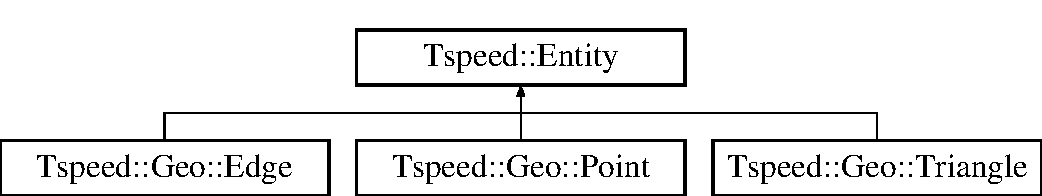
\includegraphics[height=2.000000cm]{classTspeed_1_1Entity}
\end{center}
\end{figure}
\subsection*{Public Types}
\begin{DoxyCompactItemize}
\item 
typedef unsigned int \hyperlink{classTspeed_1_1Entity_a32da920d1e9397a793b67beadd70e8fe}{Id}
\end{DoxyCompactItemize}
\subsection*{Public Member Functions}
\begin{DoxyCompactItemize}
\item 
\hyperlink{classTspeed_1_1Entity_a2d38b43574ff32961cc54430d2641d9d}{Entity} ()
\item 
bool \hyperlink{classTspeed_1_1Entity_a0254af0831b2f3d9d2e225e8720f85b9}{unassigned\-Id} () const 
\item 
bool \hyperlink{classTspeed_1_1Entity_aea3dc95515ad3a025039de1963a33a06}{unassigned\-Bc} () const 
\item 
bool \hyperlink{classTspeed_1_1Entity_ac1505ecd50daa5fcefe3bc6366977fc4}{unassigned\-Reg} () const 
\item 
\hyperlink{classTspeed_1_1Entity_a32da920d1e9397a793b67beadd70e8fe}{Id} \& \hyperlink{classTspeed_1_1Entity_a783e9df1d967686bc39f26e43f7b6c3e}{reg} ()
\item 
\hyperlink{classTspeed_1_1Entity_a32da920d1e9397a793b67beadd70e8fe}{Id} const \& \hyperlink{classTspeed_1_1Entity_a69cb766f9523627435d0ff37e511253c}{reg} () const 
\item 
\hyperlink{classTspeed_1_1Entity_a32da920d1e9397a793b67beadd70e8fe}{Id} \& \hyperlink{classTspeed_1_1Entity_abefec95d2d2511aa8ccc508a4472a339}{id} ()
\item 
\hyperlink{classTspeed_1_1Entity_a32da920d1e9397a793b67beadd70e8fe}{Id} const \& \hyperlink{classTspeed_1_1Entity_a38b1c806bcf12dfe99a66d343aff8004}{id} () const 
\item 
\hyperlink{namespaceTspeed_a301e5218199485c06d62434c719ea5e0}{Bc} \& \hyperlink{classTspeed_1_1Entity_a986365e93ee83bb0b4706260ee1c9892}{bc\-Id} ()
\item 
\hyperlink{namespaceTspeed_a301e5218199485c06d62434c719ea5e0}{Bc} const \& \hyperlink{classTspeed_1_1Entity_aab5641d64b52564729a9f55a24b9bb1b}{bc\-Id} () const 
\end{DoxyCompactItemize}
\subsection*{Protected Attributes}
\begin{DoxyCompactItemize}
\item 
\hyperlink{classTspeed_1_1Entity_a32da920d1e9397a793b67beadd70e8fe}{Id} \hyperlink{classTspeed_1_1Entity_a4c553133417f2766bd5898d2fa558374}{M\-\_\-reg}
\item 
\hyperlink{classTspeed_1_1Entity_a32da920d1e9397a793b67beadd70e8fe}{Id} \hyperlink{classTspeed_1_1Entity_a78689c259080e251d0e4ae01db20a7ba}{M\-\_\-id}
\item 
\hyperlink{namespaceTspeed_a301e5218199485c06d62434c719ea5e0}{Bc} \hyperlink{classTspeed_1_1Entity_a768810bb9f657134eac0ba66a8e0d77b}{M\-\_\-bc\-Id}
\end{DoxyCompactItemize}


\subsection{Member Typedef Documentation}
\hypertarget{classTspeed_1_1Entity_a32da920d1e9397a793b67beadd70e8fe}{\index{Tspeed\-::\-Entity@{Tspeed\-::\-Entity}!Id@{Id}}
\index{Id@{Id}!Tspeed::Entity@{Tspeed\-::\-Entity}}
\subsubsection[{Id}]{\setlength{\rightskip}{0pt plus 5cm}typedef unsigned int {\bf Tspeed\-::\-Entity\-::\-Id}}}\label{classTspeed_1_1Entity_a32da920d1e9397a793b67beadd70e8fe}


\subsection{Constructor \& Destructor Documentation}
\hypertarget{classTspeed_1_1Entity_a2d38b43574ff32961cc54430d2641d9d}{\index{Tspeed\-::\-Entity@{Tspeed\-::\-Entity}!Entity@{Entity}}
\index{Entity@{Entity}!Tspeed::Entity@{Tspeed\-::\-Entity}}
\subsubsection[{Entity}]{\setlength{\rightskip}{0pt plus 5cm}Tspeed\-::\-Entity\-::\-Entity (
\begin{DoxyParamCaption}
{}
\end{DoxyParamCaption}
)\hspace{0.3cm}{\ttfamily [inline]}}}\label{classTspeed_1_1Entity_a2d38b43574ff32961cc54430d2641d9d}


\subsection{Member Function Documentation}
\hypertarget{classTspeed_1_1Entity_a986365e93ee83bb0b4706260ee1c9892}{\index{Tspeed\-::\-Entity@{Tspeed\-::\-Entity}!bc\-Id@{bc\-Id}}
\index{bc\-Id@{bc\-Id}!Tspeed::Entity@{Tspeed\-::\-Entity}}
\subsubsection[{bc\-Id}]{\setlength{\rightskip}{0pt plus 5cm}{\bf Bc}\& Tspeed\-::\-Entity\-::bc\-Id (
\begin{DoxyParamCaption}
{}
\end{DoxyParamCaption}
)\hspace{0.3cm}{\ttfamily [inline]}}}\label{classTspeed_1_1Entity_a986365e93ee83bb0b4706260ee1c9892}
\hypertarget{classTspeed_1_1Entity_aab5641d64b52564729a9f55a24b9bb1b}{\index{Tspeed\-::\-Entity@{Tspeed\-::\-Entity}!bc\-Id@{bc\-Id}}
\index{bc\-Id@{bc\-Id}!Tspeed::Entity@{Tspeed\-::\-Entity}}
\subsubsection[{bc\-Id}]{\setlength{\rightskip}{0pt plus 5cm}{\bf Bc} const\& Tspeed\-::\-Entity\-::bc\-Id (
\begin{DoxyParamCaption}
{}
\end{DoxyParamCaption}
) const\hspace{0.3cm}{\ttfamily [inline]}}}\label{classTspeed_1_1Entity_aab5641d64b52564729a9f55a24b9bb1b}
\hypertarget{classTspeed_1_1Entity_abefec95d2d2511aa8ccc508a4472a339}{\index{Tspeed\-::\-Entity@{Tspeed\-::\-Entity}!id@{id}}
\index{id@{id}!Tspeed::Entity@{Tspeed\-::\-Entity}}
\subsubsection[{id}]{\setlength{\rightskip}{0pt plus 5cm}{\bf Id}\& Tspeed\-::\-Entity\-::id (
\begin{DoxyParamCaption}
{}
\end{DoxyParamCaption}
)\hspace{0.3cm}{\ttfamily [inline]}}}\label{classTspeed_1_1Entity_abefec95d2d2511aa8ccc508a4472a339}
\hypertarget{classTspeed_1_1Entity_a38b1c806bcf12dfe99a66d343aff8004}{\index{Tspeed\-::\-Entity@{Tspeed\-::\-Entity}!id@{id}}
\index{id@{id}!Tspeed::Entity@{Tspeed\-::\-Entity}}
\subsubsection[{id}]{\setlength{\rightskip}{0pt plus 5cm}{\bf Id} const\& Tspeed\-::\-Entity\-::id (
\begin{DoxyParamCaption}
{}
\end{DoxyParamCaption}
) const\hspace{0.3cm}{\ttfamily [inline]}}}\label{classTspeed_1_1Entity_a38b1c806bcf12dfe99a66d343aff8004}
\hypertarget{classTspeed_1_1Entity_a783e9df1d967686bc39f26e43f7b6c3e}{\index{Tspeed\-::\-Entity@{Tspeed\-::\-Entity}!reg@{reg}}
\index{reg@{reg}!Tspeed::Entity@{Tspeed\-::\-Entity}}
\subsubsection[{reg}]{\setlength{\rightskip}{0pt plus 5cm}{\bf Id}\& Tspeed\-::\-Entity\-::reg (
\begin{DoxyParamCaption}
{}
\end{DoxyParamCaption}
)\hspace{0.3cm}{\ttfamily [inline]}}}\label{classTspeed_1_1Entity_a783e9df1d967686bc39f26e43f7b6c3e}
\hypertarget{classTspeed_1_1Entity_a69cb766f9523627435d0ff37e511253c}{\index{Tspeed\-::\-Entity@{Tspeed\-::\-Entity}!reg@{reg}}
\index{reg@{reg}!Tspeed::Entity@{Tspeed\-::\-Entity}}
\subsubsection[{reg}]{\setlength{\rightskip}{0pt plus 5cm}{\bf Id} const\& Tspeed\-::\-Entity\-::reg (
\begin{DoxyParamCaption}
{}
\end{DoxyParamCaption}
) const\hspace{0.3cm}{\ttfamily [inline]}}}\label{classTspeed_1_1Entity_a69cb766f9523627435d0ff37e511253c}
\hypertarget{classTspeed_1_1Entity_aea3dc95515ad3a025039de1963a33a06}{\index{Tspeed\-::\-Entity@{Tspeed\-::\-Entity}!unassigned\-Bc@{unassigned\-Bc}}
\index{unassigned\-Bc@{unassigned\-Bc}!Tspeed::Entity@{Tspeed\-::\-Entity}}
\subsubsection[{unassigned\-Bc}]{\setlength{\rightskip}{0pt plus 5cm}bool Tspeed\-::\-Entity\-::unassigned\-Bc (
\begin{DoxyParamCaption}
{}
\end{DoxyParamCaption}
) const\hspace{0.3cm}{\ttfamily [inline]}}}\label{classTspeed_1_1Entity_aea3dc95515ad3a025039de1963a33a06}
\hypertarget{classTspeed_1_1Entity_a0254af0831b2f3d9d2e225e8720f85b9}{\index{Tspeed\-::\-Entity@{Tspeed\-::\-Entity}!unassigned\-Id@{unassigned\-Id}}
\index{unassigned\-Id@{unassigned\-Id}!Tspeed::Entity@{Tspeed\-::\-Entity}}
\subsubsection[{unassigned\-Id}]{\setlength{\rightskip}{0pt plus 5cm}bool Tspeed\-::\-Entity\-::unassigned\-Id (
\begin{DoxyParamCaption}
{}
\end{DoxyParamCaption}
) const\hspace{0.3cm}{\ttfamily [inline]}}}\label{classTspeed_1_1Entity_a0254af0831b2f3d9d2e225e8720f85b9}
\hypertarget{classTspeed_1_1Entity_ac1505ecd50daa5fcefe3bc6366977fc4}{\index{Tspeed\-::\-Entity@{Tspeed\-::\-Entity}!unassigned\-Reg@{unassigned\-Reg}}
\index{unassigned\-Reg@{unassigned\-Reg}!Tspeed::Entity@{Tspeed\-::\-Entity}}
\subsubsection[{unassigned\-Reg}]{\setlength{\rightskip}{0pt plus 5cm}bool Tspeed\-::\-Entity\-::unassigned\-Reg (
\begin{DoxyParamCaption}
{}
\end{DoxyParamCaption}
) const\hspace{0.3cm}{\ttfamily [inline]}}}\label{classTspeed_1_1Entity_ac1505ecd50daa5fcefe3bc6366977fc4}


\subsection{Member Data Documentation}
\hypertarget{classTspeed_1_1Entity_a768810bb9f657134eac0ba66a8e0d77b}{\index{Tspeed\-::\-Entity@{Tspeed\-::\-Entity}!M\-\_\-bc\-Id@{M\-\_\-bc\-Id}}
\index{M\-\_\-bc\-Id@{M\-\_\-bc\-Id}!Tspeed::Entity@{Tspeed\-::\-Entity}}
\subsubsection[{M\-\_\-bc\-Id}]{\setlength{\rightskip}{0pt plus 5cm}{\bf Bc} Tspeed\-::\-Entity\-::\-M\-\_\-bc\-Id\hspace{0.3cm}{\ttfamily [protected]}}}\label{classTspeed_1_1Entity_a768810bb9f657134eac0ba66a8e0d77b}
\hypertarget{classTspeed_1_1Entity_a78689c259080e251d0e4ae01db20a7ba}{\index{Tspeed\-::\-Entity@{Tspeed\-::\-Entity}!M\-\_\-id@{M\-\_\-id}}
\index{M\-\_\-id@{M\-\_\-id}!Tspeed::Entity@{Tspeed\-::\-Entity}}
\subsubsection[{M\-\_\-id}]{\setlength{\rightskip}{0pt plus 5cm}{\bf Id} Tspeed\-::\-Entity\-::\-M\-\_\-id\hspace{0.3cm}{\ttfamily [protected]}}}\label{classTspeed_1_1Entity_a78689c259080e251d0e4ae01db20a7ba}
\hypertarget{classTspeed_1_1Entity_a4c553133417f2766bd5898d2fa558374}{\index{Tspeed\-::\-Entity@{Tspeed\-::\-Entity}!M\-\_\-reg@{M\-\_\-reg}}
\index{M\-\_\-reg@{M\-\_\-reg}!Tspeed::Entity@{Tspeed\-::\-Entity}}
\subsubsection[{M\-\_\-reg}]{\setlength{\rightskip}{0pt plus 5cm}{\bf Id} Tspeed\-::\-Entity\-::\-M\-\_\-reg\hspace{0.3cm}{\ttfamily [protected]}}}\label{classTspeed_1_1Entity_a4c553133417f2766bd5898d2fa558374}


The documentation for this class was generated from the following file\-:\begin{DoxyCompactItemize}
\item 
lib/include/\hyperlink{Geometry_8hpp}{Geometry.\-hpp}\end{DoxyCompactItemize}

\hypertarget{classTspeed_1_1FESpace}{\section{Tspeed\-:\-:F\-E\-Space$<$ N, Q, S $>$ Class Template Reference}
\label{classTspeed_1_1FESpace}\index{Tspeed\-::\-F\-E\-Space$<$ N, Q, S $>$@{Tspeed\-::\-F\-E\-Space$<$ N, Q, S $>$}}
}


Functional space.  




{\ttfamily \#include $<$F\-E\-Space.\-hpp$>$}

\subsection*{Public Member Functions}
\begin{DoxyCompactItemize}
\item 
\hyperlink{classTspeed_1_1FESpace_aecf45c5fb39b7df60599d2d055c9506d}{F\-E\-Space} (\hyperlink{namespaceTspeed_a7367a01365c4cc2c1a09305b3effc4e8}{Mesh\-\_\-ptr} m)
\begin{DoxyCompactList}\small\item\em Constructor from the mesh. \end{DoxyCompactList}\item 
virtual \hyperlink{classTspeed_1_1FESpace_ae1f9e4f07e24640e68a138c1d11ad900}{$\sim$\-F\-E\-Space} ()
\item 
\hyperlink{namespaceTspeed_a7367a01365c4cc2c1a09305b3effc4e8}{Mesh\-\_\-ptr} \hyperlink{classTspeed_1_1FESpace_a52581134e398195d098ad4f1985a4cbb}{mesh} () const 
\begin{DoxyCompactList}\small\item\em Get pointer ot mesh. \end{DoxyCompactList}\item 
Q const \& \hyperlink{classTspeed_1_1FESpace_a118bd2d5becbd61c593efa546a525992}{quad} () const 
\begin{DoxyCompactList}\small\item\em Get quadrature rule. \end{DoxyCompactList}\item 
\hyperlink{classTspeed_1_1ShapeFunction}{Shape\-Function}$<$ N $>$ const \& \hyperlink{classTspeed_1_1FESpace_ac9829cde89c0e1a5252925c1e9322d47}{shape} () const 
\begin{DoxyCompactList}\small\item\em Get Shapefunction. \end{DoxyCompactList}\item 
unsigned int \hyperlink{classTspeed_1_1FESpace_ae32c88a6615cefdf1273e2525a62fcfe}{nln} () const 
\begin{DoxyCompactList}\small\item\em Number of degrees of freedom per element. \end{DoxyCompactList}\item 
unsigned int \hyperlink{classTspeed_1_1FESpace_a3e6a6031a7b2033f90ce1d0f3b6a378d}{ne} () const 
\begin{DoxyCompactList}\small\item\em Number of elements in the mesh. \end{DoxyCompactList}\item 
Eigen\-::\-Vector2d \hyperlink{classTspeed_1_1FESpace_a5b658aa075508f9ead3b4cac4743bfac}{grad} (unsigned int k, unsigned int i) const 
\begin{DoxyCompactList}\small\item\em Get value of the gradient of the basis function i on quadrature point k. \end{DoxyCompactList}\item 
Eigen\-::\-Vector\-Xd \hyperlink{classTspeed_1_1FESpace_afee2268392456e7b872a8c3d77f732c7}{b\-\_\-edge} (unsigned int k, unsigned int iedg) const 
\begin{DoxyCompactList}\small\item\em Get value of all basis function on quadrature node k, on edge iedg. \end{DoxyCompactList}\item 
Eigen\-::\-Vector2d \hyperlink{classTspeed_1_1FESpace_aee7e220399d909994b7b91f4fa82f1ca}{g\-\_\-edge} (unsigned int k, unsigned int i, unsigned short int edg) const 
\begin{DoxyCompactList}\small\item\em value of the gradient of basis function i, on edge edg, quadrature node k \end{DoxyCompactList}\item 
Eigen\-::\-Vector\-Xd \hyperlink{classTspeed_1_1FESpace_a37f34239467d7a425060025e9b794160}{inverse\-\_\-transform} (std\-::function$<$ std\-::array$<$ double, 2 $>$(double, double)$>$ const \&fun) const 
\begin{DoxyCompactList}\small\item\em Transform a function $u(x,y)$ into its expantion modes $\hat{u}_i$ s.\-t. \[ \sum_i \hat{u}_i\psi_i(x,y) = u(x,y) \]. \end{DoxyCompactList}\item 
double \hyperlink{classTspeed_1_1FESpace_a82f14839c97266bc4ba1448b59398aad}{L2error} (std\-::function$<$ std\-::array$<$ double, 2 $>$(double, double)$>$ const \&uex, Eigen\-::\-Vector\-Xd const \&uh) const 
\begin{DoxyCompactList}\small\item\em L2 norm of the difference uex-\/uh. \end{DoxyCompactList}\item 
Eigen\-::\-Vector\-Xd \hyperlink{classTspeed_1_1FESpace_a0336e65ff3cbd3e2ffa948750e3ce805}{loc\-\_\-rhs} (\hyperlink{classTspeed_1_1Geo_1_1Triangle}{Geo\-::\-Triangle} const \&ie, std\-::function$<$ std\-::array$<$ double, 2 $>$(double, double)$>$ const \&fun) const 
\begin{DoxyCompactList}\small\item\em Integration of a function against all basis function, in triangle ie, i.\-e. \[ l_i = \int_\mathrm{ie} f \psi_i \]. \end{DoxyCompactList}\item 
void \hyperlink{classTspeed_1_1FESpace_ad92a40f39edfb095b42bc6389b11d78f}{points\-\_\-out} (std\-::string const \&fname) const 
\begin{DoxyCompactList}\small\item\em Write a set of points of the mesh to file. \end{DoxyCompactList}\item 
void \hyperlink{classTspeed_1_1FESpace_a72a024911d1a650c078e0bfc66ccc837}{field\-\_\-out} (std\-::string const \&fname, Eigen\-::\-Vector\-Xd const \&uh, unsigned int step) const 
\begin{DoxyCompactList}\small\item\em Write a field to file, on the points given by points\-\_\-out. \end{DoxyCompactList}\item 
Eigen\-::\-Matrix\-Xd \hyperlink{classTspeed_1_1FESpace_ab78f6ab6c66a321d925f5f989a8ded1f}{base\-\_\-mass} () const 
\begin{DoxyCompactList}\small\item\em Evaluate the mass matrix $\mathbf{M}$ s.\-t. \[ M_{ij} = \int_{\mathcal{T}^2} \psi_i \psi_j\]. \end{DoxyCompactList}\item 
Eigen\-::\-Matrix\-Xd \hyperlink{classTspeed_1_1FESpace_a0a6366236da7e30ee9f9c560c9d077f1}{base\-\_\-invmass} () const 
\begin{DoxyCompactList}\small\item\em Evaluate the inverse of the mass matrix $ \mathbf{M}^{-1} $. \end{DoxyCompactList}\end{DoxyCompactItemize}
\subsection*{Public Attributes}
\begin{DoxyCompactItemize}
\item 
\hyperlink{classTspeed_1_1FESpace_ac3dd8d1e0ee8533ee01b69775e40f76a}{E\-I\-G\-E\-N\-\_\-\-M\-A\-K\-E\-\_\-\-A\-L\-I\-G\-N\-E\-D\-\_\-\-O\-P\-E\-R\-A\-T\-O\-R\-\_\-\-N\-E\-W}
\end{DoxyCompactItemize}


\subsection{Detailed Description}
\subsubsection*{template$<$int N, typename Q = Gauss$<$\-N+1$>$, typename S = Dubiner$<$\-N$>$$>$class Tspeed\-::\-F\-E\-Space$<$ N, Q, S $>$}

Functional space. 


\begin{DoxyTemplParams}{Template Parameters}
{\em N} & order of the polynomials \\
\hline
{\em Q} & quadrature rule \\
\hline
{\em S} & basis functions \\
\hline
\end{DoxyTemplParams}


\subsection{Constructor \& Destructor Documentation}
\hypertarget{classTspeed_1_1FESpace_aecf45c5fb39b7df60599d2d055c9506d}{\index{Tspeed\-::\-F\-E\-Space@{Tspeed\-::\-F\-E\-Space}!F\-E\-Space@{F\-E\-Space}}
\index{F\-E\-Space@{F\-E\-Space}!Tspeed::FESpace@{Tspeed\-::\-F\-E\-Space}}
\subsubsection[{F\-E\-Space}]{\setlength{\rightskip}{0pt plus 5cm}template$<$int N, typename Q , typename S $>$ {\bf Tspeed\-::\-F\-E\-Space}$<$ N, Q, S $>$\-::{\bf F\-E\-Space} (
\begin{DoxyParamCaption}
\item[{{\bf Mesh\-\_\-ptr}}]{m}
\end{DoxyParamCaption}
)\hspace{0.3cm}{\ttfamily [explicit]}}}\label{classTspeed_1_1FESpace_aecf45c5fb39b7df60599d2d055c9506d}


Constructor from the mesh. 


\begin{DoxyParams}{Parameters}
{\em m} & shared pointer to \hyperlink{classTspeed_1_1Mesh}{Mesh} \\
\hline
\end{DoxyParams}
\hypertarget{classTspeed_1_1FESpace_ae1f9e4f07e24640e68a138c1d11ad900}{\index{Tspeed\-::\-F\-E\-Space@{Tspeed\-::\-F\-E\-Space}!$\sim$\-F\-E\-Space@{$\sim$\-F\-E\-Space}}
\index{$\sim$\-F\-E\-Space@{$\sim$\-F\-E\-Space}!Tspeed::FESpace@{Tspeed\-::\-F\-E\-Space}}
\subsubsection[{$\sim$\-F\-E\-Space}]{\setlength{\rightskip}{0pt plus 5cm}template$<$int N, typename Q  = Gauss$<$\-N+1$>$, typename S  = Dubiner$<$\-N$>$$>$ virtual {\bf Tspeed\-::\-F\-E\-Space}$<$ N, Q, S $>$\-::$\sim${\bf F\-E\-Space} (
\begin{DoxyParamCaption}
{}
\end{DoxyParamCaption}
)\hspace{0.3cm}{\ttfamily [inline]}, {\ttfamily [virtual]}}}\label{classTspeed_1_1FESpace_ae1f9e4f07e24640e68a138c1d11ad900}


\subsection{Member Function Documentation}
\hypertarget{classTspeed_1_1FESpace_afee2268392456e7b872a8c3d77f732c7}{\index{Tspeed\-::\-F\-E\-Space@{Tspeed\-::\-F\-E\-Space}!b\-\_\-edge@{b\-\_\-edge}}
\index{b\-\_\-edge@{b\-\_\-edge}!Tspeed::FESpace@{Tspeed\-::\-F\-E\-Space}}
\subsubsection[{b\-\_\-edge}]{\setlength{\rightskip}{0pt plus 5cm}template$<$int N, typename Q  = Gauss$<$\-N+1$>$, typename S  = Dubiner$<$\-N$>$$>$ Eigen\-::\-Vector\-Xd {\bf Tspeed\-::\-F\-E\-Space}$<$ N, Q, S $>$\-::b\-\_\-edge (
\begin{DoxyParamCaption}
\item[{unsigned int}]{k, }
\item[{unsigned int}]{iedg}
\end{DoxyParamCaption}
) const\hspace{0.3cm}{\ttfamily [inline]}}}\label{classTspeed_1_1FESpace_afee2268392456e7b872a8c3d77f732c7}


Get value of all basis function on quadrature node k, on edge iedg. 


\begin{DoxyParams}{Parameters}
{\em k} & index of the quadrature point \\
\hline
{\em iedg} & index of the edge (=0,1,2)\\
\hline
\end{DoxyParams}
\begin{DoxyReturn}{Returns}
vector of all the values 
\end{DoxyReturn}
\hypertarget{classTspeed_1_1FESpace_a0a6366236da7e30ee9f9c560c9d077f1}{\index{Tspeed\-::\-F\-E\-Space@{Tspeed\-::\-F\-E\-Space}!base\-\_\-invmass@{base\-\_\-invmass}}
\index{base\-\_\-invmass@{base\-\_\-invmass}!Tspeed::FESpace@{Tspeed\-::\-F\-E\-Space}}
\subsubsection[{base\-\_\-invmass}]{\setlength{\rightskip}{0pt plus 5cm}template$<$int N, typename Q  = Gauss$<$\-N+1$>$, typename S  = Dubiner$<$\-N$>$$>$ Eigen\-::\-Matrix\-Xd {\bf Tspeed\-::\-F\-E\-Space}$<$ N, Q, S $>$\-::base\-\_\-invmass (
\begin{DoxyParamCaption}
{}
\end{DoxyParamCaption}
) const\hspace{0.3cm}{\ttfamily [inline]}}}\label{classTspeed_1_1FESpace_a0a6366236da7e30ee9f9c560c9d077f1}


Evaluate the inverse of the mass matrix $ \mathbf{M}^{-1} $. 

\begin{DoxyReturn}{Returns}
$ \mathbf{M}^{-1} $ 
\end{DoxyReturn}
\hypertarget{classTspeed_1_1FESpace_ab78f6ab6c66a321d925f5f989a8ded1f}{\index{Tspeed\-::\-F\-E\-Space@{Tspeed\-::\-F\-E\-Space}!base\-\_\-mass@{base\-\_\-mass}}
\index{base\-\_\-mass@{base\-\_\-mass}!Tspeed::FESpace@{Tspeed\-::\-F\-E\-Space}}
\subsubsection[{base\-\_\-mass}]{\setlength{\rightskip}{0pt plus 5cm}template$<$int N, typename Q  = Gauss$<$\-N+1$>$, typename S  = Dubiner$<$\-N$>$$>$ Eigen\-::\-Matrix\-Xd {\bf Tspeed\-::\-F\-E\-Space}$<$ N, Q, S $>$\-::base\-\_\-mass (
\begin{DoxyParamCaption}
{}
\end{DoxyParamCaption}
) const\hspace{0.3cm}{\ttfamily [inline]}}}\label{classTspeed_1_1FESpace_ab78f6ab6c66a321d925f5f989a8ded1f}


Evaluate the mass matrix $\mathbf{M}$ s.\-t. \[ M_{ij} = \int_{\mathcal{T}^2} \psi_i \psi_j\]. 

\begin{DoxyReturn}{Returns}
the matrix $ \mathbf{M} $ 
\end{DoxyReturn}
\hypertarget{classTspeed_1_1FESpace_a72a024911d1a650c078e0bfc66ccc837}{\index{Tspeed\-::\-F\-E\-Space@{Tspeed\-::\-F\-E\-Space}!field\-\_\-out@{field\-\_\-out}}
\index{field\-\_\-out@{field\-\_\-out}!Tspeed::FESpace@{Tspeed\-::\-F\-E\-Space}}
\subsubsection[{field\-\_\-out}]{\setlength{\rightskip}{0pt plus 5cm}template$<$int N, typename Q , typename S $>$ void {\bf Tspeed\-::\-F\-E\-Space}$<$ N, Q, S $>$\-::field\-\_\-out (
\begin{DoxyParamCaption}
\item[{std\-::string const \&}]{fname, }
\item[{Eigen\-::\-Vector\-Xd const \&}]{uh, }
\item[{unsigned int}]{step}
\end{DoxyParamCaption}
) const}}\label{classTspeed_1_1FESpace_a72a024911d1a650c078e0bfc66ccc837}


Write a field to file, on the points given by points\-\_\-out. 


\begin{DoxyParams}{Parameters}
{\em fname} & name of the output file \\
\hline
{\em uh} & vector of the coefficients of a F\-E function \\
\hline
{\em step} & the time step (gets appended to the file name) \\
\hline
\end{DoxyParams}
\hypertarget{classTspeed_1_1FESpace_aee7e220399d909994b7b91f4fa82f1ca}{\index{Tspeed\-::\-F\-E\-Space@{Tspeed\-::\-F\-E\-Space}!g\-\_\-edge@{g\-\_\-edge}}
\index{g\-\_\-edge@{g\-\_\-edge}!Tspeed::FESpace@{Tspeed\-::\-F\-E\-Space}}
\subsubsection[{g\-\_\-edge}]{\setlength{\rightskip}{0pt plus 5cm}template$<$int N, typename Q  = Gauss$<$\-N+1$>$, typename S  = Dubiner$<$\-N$>$$>$ Eigen\-::\-Vector2d {\bf Tspeed\-::\-F\-E\-Space}$<$ N, Q, S $>$\-::g\-\_\-edge (
\begin{DoxyParamCaption}
\item[{unsigned int}]{k, }
\item[{unsigned int}]{i, }
\item[{unsigned short int}]{edg}
\end{DoxyParamCaption}
) const\hspace{0.3cm}{\ttfamily [inline]}}}\label{classTspeed_1_1FESpace_aee7e220399d909994b7b91f4fa82f1ca}


value of the gradient of basis function i, on edge edg, quadrature node k 


\begin{DoxyParams}{Parameters}
{\em k} & index of the quadrature node \\
\hline
{\em i} & indec of the basis function \\
\hline
{\em edg} & edg number\\
\hline
\end{DoxyParams}
\begin{DoxyReturn}{Returns}
a vector with the x and y derivatives 
\end{DoxyReturn}
\hypertarget{classTspeed_1_1FESpace_a5b658aa075508f9ead3b4cac4743bfac}{\index{Tspeed\-::\-F\-E\-Space@{Tspeed\-::\-F\-E\-Space}!grad@{grad}}
\index{grad@{grad}!Tspeed::FESpace@{Tspeed\-::\-F\-E\-Space}}
\subsubsection[{grad}]{\setlength{\rightskip}{0pt plus 5cm}template$<$int N, typename Q  = Gauss$<$\-N+1$>$, typename S  = Dubiner$<$\-N$>$$>$ Eigen\-::\-Vector2d {\bf Tspeed\-::\-F\-E\-Space}$<$ N, Q, S $>$\-::grad (
\begin{DoxyParamCaption}
\item[{unsigned int}]{k, }
\item[{unsigned int}]{i}
\end{DoxyParamCaption}
) const\hspace{0.3cm}{\ttfamily [inline]}}}\label{classTspeed_1_1FESpace_a5b658aa075508f9ead3b4cac4743bfac}


Get value of the gradient of the basis function i on quadrature point k. 


\begin{DoxyParams}{Parameters}
{\em k} & index of the quadrature node \\
\hline
{\em i} & index of the basis function\\
\hline
\end{DoxyParams}
\begin{DoxyReturn}{Returns}
A vector with the x and y derivatives 
\end{DoxyReturn}
\hypertarget{classTspeed_1_1FESpace_a37f34239467d7a425060025e9b794160}{\index{Tspeed\-::\-F\-E\-Space@{Tspeed\-::\-F\-E\-Space}!inverse\-\_\-transform@{inverse\-\_\-transform}}
\index{inverse\-\_\-transform@{inverse\-\_\-transform}!Tspeed::FESpace@{Tspeed\-::\-F\-E\-Space}}
\subsubsection[{inverse\-\_\-transform}]{\setlength{\rightskip}{0pt plus 5cm}template$<$int N, typename Q , typename S $>$ Eigen\-::\-Vector\-Xd {\bf Tspeed\-::\-F\-E\-Space}$<$ N, Q, S $>$\-::inverse\-\_\-transform (
\begin{DoxyParamCaption}
\item[{std\-::function$<$ std\-::array$<$ double, 2 $>$(double, double)$>$ const \&}]{fun}
\end{DoxyParamCaption}
) const}}\label{classTspeed_1_1FESpace_a37f34239467d7a425060025e9b794160}


Transform a function $u(x,y)$ into its expantion modes $\hat{u}_i$ s.\-t. \[ \sum_i \hat{u}_i\psi_i(x,y) = u(x,y) \]. 


\begin{DoxyParams}{Parameters}
{\em fun} & the function\\
\hline
\end{DoxyParams}
\begin{DoxyReturn}{Returns}
the vector of $\hat{u}_i$ 
\end{DoxyReturn}
\hypertarget{classTspeed_1_1FESpace_a82f14839c97266bc4ba1448b59398aad}{\index{Tspeed\-::\-F\-E\-Space@{Tspeed\-::\-F\-E\-Space}!L2error@{L2error}}
\index{L2error@{L2error}!Tspeed::FESpace@{Tspeed\-::\-F\-E\-Space}}
\subsubsection[{L2error}]{\setlength{\rightskip}{0pt plus 5cm}template$<$int N, typename Q , typename S $>$ double {\bf Tspeed\-::\-F\-E\-Space}$<$ N, Q, S $>$\-::L2error (
\begin{DoxyParamCaption}
\item[{std\-::function$<$ std\-::array$<$ double, 2 $>$(double, double)$>$ const \&}]{uex, }
\item[{Eigen\-::\-Vector\-Xd const \&}]{uh}
\end{DoxyParamCaption}
) const}}\label{classTspeed_1_1FESpace_a82f14839c97266bc4ba1448b59398aad}


L2 norm of the difference uex-\/uh. 


\begin{DoxyParams}{Parameters}
{\em uex} & A function \\
\hline
{\em uh} & A vector of expansion modes\\
\hline
\end{DoxyParams}
\begin{DoxyReturn}{Returns}
The norm 
\end{DoxyReturn}
\hypertarget{classTspeed_1_1FESpace_a0336e65ff3cbd3e2ffa948750e3ce805}{\index{Tspeed\-::\-F\-E\-Space@{Tspeed\-::\-F\-E\-Space}!loc\-\_\-rhs@{loc\-\_\-rhs}}
\index{loc\-\_\-rhs@{loc\-\_\-rhs}!Tspeed::FESpace@{Tspeed\-::\-F\-E\-Space}}
\subsubsection[{loc\-\_\-rhs}]{\setlength{\rightskip}{0pt plus 5cm}template$<$int N, typename Q  = Gauss$<$\-N+1$>$, typename S  = Dubiner$<$\-N$>$$>$ Eigen\-::\-Vector\-Xd {\bf Tspeed\-::\-F\-E\-Space}$<$ N, Q, S $>$\-::loc\-\_\-rhs (
\begin{DoxyParamCaption}
\item[{{\bf Geo\-::\-Triangle} const \&}]{ie, }
\item[{std\-::function$<$ std\-::array$<$ double, 2 $>$(double, double)$>$ const \&}]{fun}
\end{DoxyParamCaption}
) const\hspace{0.3cm}{\ttfamily [inline]}}}\label{classTspeed_1_1FESpace_a0336e65ff3cbd3e2ffa948750e3ce805}


Integration of a function against all basis function, in triangle ie, i.\-e. \[ l_i = \int_\mathrm{ie} f \psi_i \]. 


\begin{DoxyParams}{Parameters}
{\em ie} & the index of the triangle \\
\hline
{\em fun} & the function to be integrated\\
\hline
\end{DoxyParams}
\begin{DoxyReturn}{Returns}
the vector made by $ l_i $ 
\end{DoxyReturn}
\hypertarget{classTspeed_1_1FESpace_a52581134e398195d098ad4f1985a4cbb}{\index{Tspeed\-::\-F\-E\-Space@{Tspeed\-::\-F\-E\-Space}!mesh@{mesh}}
\index{mesh@{mesh}!Tspeed::FESpace@{Tspeed\-::\-F\-E\-Space}}
\subsubsection[{mesh}]{\setlength{\rightskip}{0pt plus 5cm}template$<$int N, typename Q  = Gauss$<$\-N+1$>$, typename S  = Dubiner$<$\-N$>$$>$ {\bf Mesh\-\_\-ptr} {\bf Tspeed\-::\-F\-E\-Space}$<$ N, Q, S $>$\-::mesh (
\begin{DoxyParamCaption}
{}
\end{DoxyParamCaption}
) const\hspace{0.3cm}{\ttfamily [inline]}}}\label{classTspeed_1_1FESpace_a52581134e398195d098ad4f1985a4cbb}


Get pointer ot mesh. 

\begin{DoxyReturn}{Returns}
pointer to the mesh 
\end{DoxyReturn}
\hypertarget{classTspeed_1_1FESpace_a3e6a6031a7b2033f90ce1d0f3b6a378d}{\index{Tspeed\-::\-F\-E\-Space@{Tspeed\-::\-F\-E\-Space}!ne@{ne}}
\index{ne@{ne}!Tspeed::FESpace@{Tspeed\-::\-F\-E\-Space}}
\subsubsection[{ne}]{\setlength{\rightskip}{0pt plus 5cm}template$<$int N, typename Q  = Gauss$<$\-N+1$>$, typename S  = Dubiner$<$\-N$>$$>$ unsigned int {\bf Tspeed\-::\-F\-E\-Space}$<$ N, Q, S $>$\-::ne (
\begin{DoxyParamCaption}
{}
\end{DoxyParamCaption}
) const\hspace{0.3cm}{\ttfamily [inline]}}}\label{classTspeed_1_1FESpace_a3e6a6031a7b2033f90ce1d0f3b6a378d}


Number of elements in the mesh. 

\hypertarget{classTspeed_1_1FESpace_ae32c88a6615cefdf1273e2525a62fcfe}{\index{Tspeed\-::\-F\-E\-Space@{Tspeed\-::\-F\-E\-Space}!nln@{nln}}
\index{nln@{nln}!Tspeed::FESpace@{Tspeed\-::\-F\-E\-Space}}
\subsubsection[{nln}]{\setlength{\rightskip}{0pt plus 5cm}template$<$int N, typename Q  = Gauss$<$\-N+1$>$, typename S  = Dubiner$<$\-N$>$$>$ unsigned int {\bf Tspeed\-::\-F\-E\-Space}$<$ N, Q, S $>$\-::nln (
\begin{DoxyParamCaption}
{}
\end{DoxyParamCaption}
) const\hspace{0.3cm}{\ttfamily [inline]}}}\label{classTspeed_1_1FESpace_ae32c88a6615cefdf1273e2525a62fcfe}


Number of degrees of freedom per element. 

\hypertarget{classTspeed_1_1FESpace_ad92a40f39edfb095b42bc6389b11d78f}{\index{Tspeed\-::\-F\-E\-Space@{Tspeed\-::\-F\-E\-Space}!points\-\_\-out@{points\-\_\-out}}
\index{points\-\_\-out@{points\-\_\-out}!Tspeed::FESpace@{Tspeed\-::\-F\-E\-Space}}
\subsubsection[{points\-\_\-out}]{\setlength{\rightskip}{0pt plus 5cm}template$<$int N, typename Q , typename S $>$ void {\bf Tspeed\-::\-F\-E\-Space}$<$ N, Q, S $>$\-::points\-\_\-out (
\begin{DoxyParamCaption}
\item[{std\-::string const \&}]{fname}
\end{DoxyParamCaption}
) const}}\label{classTspeed_1_1FESpace_ad92a40f39edfb095b42bc6389b11d78f}


Write a set of points of the mesh to file. 


\begin{DoxyParams}{Parameters}
{\em fname} & name of the outpu file \\
\hline
\end{DoxyParams}
\hypertarget{classTspeed_1_1FESpace_a118bd2d5becbd61c593efa546a525992}{\index{Tspeed\-::\-F\-E\-Space@{Tspeed\-::\-F\-E\-Space}!quad@{quad}}
\index{quad@{quad}!Tspeed::FESpace@{Tspeed\-::\-F\-E\-Space}}
\subsubsection[{quad}]{\setlength{\rightskip}{0pt plus 5cm}template$<$int N, typename Q  = Gauss$<$\-N+1$>$, typename S  = Dubiner$<$\-N$>$$>$ Q const\& {\bf Tspeed\-::\-F\-E\-Space}$<$ N, Q, S $>$\-::quad (
\begin{DoxyParamCaption}
{}
\end{DoxyParamCaption}
) const\hspace{0.3cm}{\ttfamily [inline]}}}\label{classTspeed_1_1FESpace_a118bd2d5becbd61c593efa546a525992}


Get quadrature rule. 

\hypertarget{classTspeed_1_1FESpace_ac9829cde89c0e1a5252925c1e9322d47}{\index{Tspeed\-::\-F\-E\-Space@{Tspeed\-::\-F\-E\-Space}!shape@{shape}}
\index{shape@{shape}!Tspeed::FESpace@{Tspeed\-::\-F\-E\-Space}}
\subsubsection[{shape}]{\setlength{\rightskip}{0pt plus 5cm}template$<$int N, typename Q  = Gauss$<$\-N+1$>$, typename S  = Dubiner$<$\-N$>$$>$ {\bf Shape\-Function}$<$N$>$ const\& {\bf Tspeed\-::\-F\-E\-Space}$<$ N, Q, S $>$\-::shape (
\begin{DoxyParamCaption}
{}
\end{DoxyParamCaption}
) const\hspace{0.3cm}{\ttfamily [inline]}}}\label{classTspeed_1_1FESpace_ac9829cde89c0e1a5252925c1e9322d47}


Get Shapefunction. 



\subsection{Member Data Documentation}
\hypertarget{classTspeed_1_1FESpace_ac3dd8d1e0ee8533ee01b69775e40f76a}{\index{Tspeed\-::\-F\-E\-Space@{Tspeed\-::\-F\-E\-Space}!E\-I\-G\-E\-N\-\_\-\-M\-A\-K\-E\-\_\-\-A\-L\-I\-G\-N\-E\-D\-\_\-\-O\-P\-E\-R\-A\-T\-O\-R\-\_\-\-N\-E\-W@{E\-I\-G\-E\-N\-\_\-\-M\-A\-K\-E\-\_\-\-A\-L\-I\-G\-N\-E\-D\-\_\-\-O\-P\-E\-R\-A\-T\-O\-R\-\_\-\-N\-E\-W}}
\index{E\-I\-G\-E\-N\-\_\-\-M\-A\-K\-E\-\_\-\-A\-L\-I\-G\-N\-E\-D\-\_\-\-O\-P\-E\-R\-A\-T\-O\-R\-\_\-\-N\-E\-W@{E\-I\-G\-E\-N\-\_\-\-M\-A\-K\-E\-\_\-\-A\-L\-I\-G\-N\-E\-D\-\_\-\-O\-P\-E\-R\-A\-T\-O\-R\-\_\-\-N\-E\-W}!Tspeed::FESpace@{Tspeed\-::\-F\-E\-Space}}
\subsubsection[{E\-I\-G\-E\-N\-\_\-\-M\-A\-K\-E\-\_\-\-A\-L\-I\-G\-N\-E\-D\-\_\-\-O\-P\-E\-R\-A\-T\-O\-R\-\_\-\-N\-E\-W}]{\setlength{\rightskip}{0pt plus 5cm}template$<$int N, typename Q  = Gauss$<$\-N+1$>$, typename S  = Dubiner$<$\-N$>$$>$ {\bf Tspeed\-::\-F\-E\-Space}$<$ N, Q, S $>$\-::E\-I\-G\-E\-N\-\_\-\-M\-A\-K\-E\-\_\-\-A\-L\-I\-G\-N\-E\-D\-\_\-\-O\-P\-E\-R\-A\-T\-O\-R\-\_\-\-N\-E\-W}}\label{classTspeed_1_1FESpace_ac3dd8d1e0ee8533ee01b69775e40f76a}


The documentation for this class was generated from the following files\-:\begin{DoxyCompactItemize}
\item 
lib/include/\hyperlink{FESpace_8hpp}{F\-E\-Space.\-hpp}\item 
lib/include/\hyperlink{FESpace__imp_8hpp}{F\-E\-Space\-\_\-imp.\-hpp}\end{DoxyCompactItemize}

\hypertarget{classTspeed_1_1Force}{\section{Tspeed\-:\-:Force Class Reference}
\label{classTspeed_1_1Force}\index{Tspeed\-::\-Force@{Tspeed\-::\-Force}}
}


virtual base class for forces  




{\ttfamily \#include $<$Force.\-hpp$>$}

Inheritance diagram for Tspeed\-:\-:Force\-:\begin{figure}[H]
\begin{center}
\leavevmode
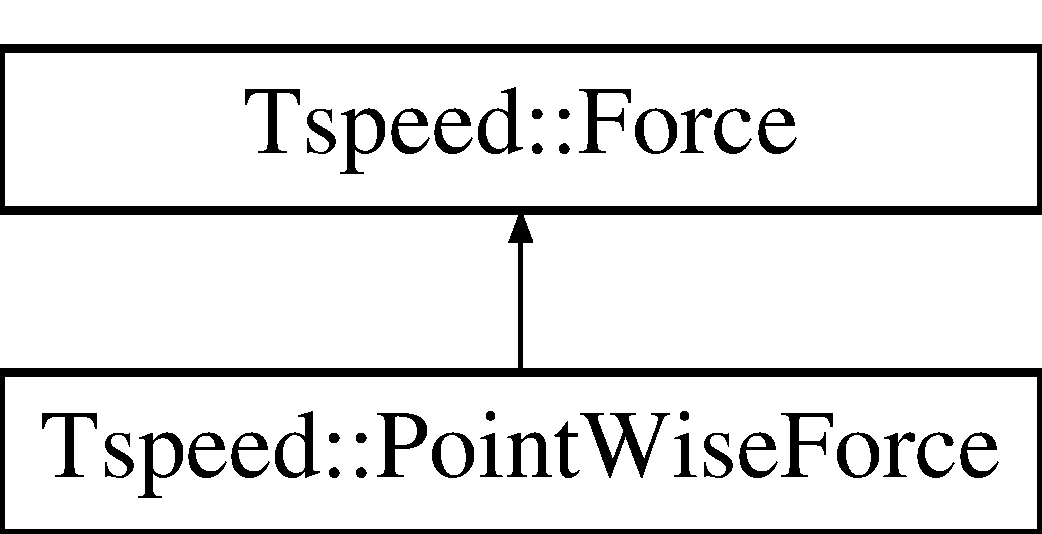
\includegraphics[height=2.000000cm]{classTspeed_1_1Force}
\end{center}
\end{figure}
\subsection*{Public Types}
\begin{DoxyCompactItemize}
\item 
typedef Eigen\-::\-Sparse\-Vector\\*
$<$ double $>$ \hyperlink{classTspeed_1_1Force_a5f4cd0ccfce951a7edded01c87ba6fb6}{S\-P\-Vec}
\item 
typedef Eigen\-::\-Vector\-Xd \hyperlink{classTspeed_1_1Force_ab33d4f6bed9bf9a136afd1ac5a918c93}{Vec}
\end{DoxyCompactItemize}
\subsection*{Public Member Functions}
\begin{DoxyCompactItemize}
\item 
\hyperlink{classTspeed_1_1Force_a1763e5fb61e4ef56be851800d854c96d}{Force} ()
\item 
\hyperlink{classTspeed_1_1Force_a2e90175e9cde9e42844ecad2e9123fbd}{Force} (std\-::function$<$ std\-::array$<$ double, 2 $>$(const double \&)$>$ const \&fun)
\begin{DoxyCompactList}\small\item\em Constructor, taking the function (time dependent) \end{DoxyCompactList}\item 
virtual \hyperlink{classTspeed_1_1Force_aa4789eaa544d8b37d25873a6c8aede55}{$\sim$\-Force} ()
\item 
virtual \hyperlink{classTspeed_1_1Force_ab33d4f6bed9bf9a136afd1ac5a918c93}{Vec} \hyperlink{classTspeed_1_1Force_ac174525b11c7c6a490411d00330a3564}{eval} (const double \&) const =0
\end{DoxyCompactItemize}
\subsection*{Protected Attributes}
\begin{DoxyCompactItemize}
\item 
std\-::function$<$ std\-::array\\*
$<$ double, 2 $>$const double \&)$>$ \hyperlink{classTspeed_1_1Force_a71c3dbf2cbca2fe0c4db4db1673794e6}{M\-\_\-f}
\end{DoxyCompactItemize}


\subsection{Detailed Description}
virtual base class for forces 

\subsection{Member Typedef Documentation}
\hypertarget{classTspeed_1_1Force_a5f4cd0ccfce951a7edded01c87ba6fb6}{\index{Tspeed\-::\-Force@{Tspeed\-::\-Force}!S\-P\-Vec@{S\-P\-Vec}}
\index{S\-P\-Vec@{S\-P\-Vec}!Tspeed::Force@{Tspeed\-::\-Force}}
\subsubsection[{S\-P\-Vec}]{\setlength{\rightskip}{0pt plus 5cm}typedef Eigen\-::\-Sparse\-Vector$<$double$>$ {\bf Tspeed\-::\-Force\-::\-S\-P\-Vec}}}\label{classTspeed_1_1Force_a5f4cd0ccfce951a7edded01c87ba6fb6}
\hypertarget{classTspeed_1_1Force_ab33d4f6bed9bf9a136afd1ac5a918c93}{\index{Tspeed\-::\-Force@{Tspeed\-::\-Force}!Vec@{Vec}}
\index{Vec@{Vec}!Tspeed::Force@{Tspeed\-::\-Force}}
\subsubsection[{Vec}]{\setlength{\rightskip}{0pt plus 5cm}typedef Eigen\-::\-Vector\-Xd {\bf Tspeed\-::\-Force\-::\-Vec}}}\label{classTspeed_1_1Force_ab33d4f6bed9bf9a136afd1ac5a918c93}


\subsection{Constructor \& Destructor Documentation}
\hypertarget{classTspeed_1_1Force_a1763e5fb61e4ef56be851800d854c96d}{\index{Tspeed\-::\-Force@{Tspeed\-::\-Force}!Force@{Force}}
\index{Force@{Force}!Tspeed::Force@{Tspeed\-::\-Force}}
\subsubsection[{Force}]{\setlength{\rightskip}{0pt plus 5cm}Tspeed\-::\-Force\-::\-Force (
\begin{DoxyParamCaption}
{}
\end{DoxyParamCaption}
)\hspace{0.3cm}{\ttfamily [inline]}}}\label{classTspeed_1_1Force_a1763e5fb61e4ef56be851800d854c96d}
\hypertarget{classTspeed_1_1Force_a2e90175e9cde9e42844ecad2e9123fbd}{\index{Tspeed\-::\-Force@{Tspeed\-::\-Force}!Force@{Force}}
\index{Force@{Force}!Tspeed::Force@{Tspeed\-::\-Force}}
\subsubsection[{Force}]{\setlength{\rightskip}{0pt plus 5cm}Tspeed\-::\-Force\-::\-Force (
\begin{DoxyParamCaption}
\item[{std\-::function$<$ std\-::array$<$ double, 2 $>$(const double \&)$>$ const \&}]{fun}
\end{DoxyParamCaption}
)}}\label{classTspeed_1_1Force_a2e90175e9cde9e42844ecad2e9123fbd}


Constructor, taking the function (time dependent) 


\begin{DoxyParams}{Parameters}
{\em fun} & The function \\
\hline
\end{DoxyParams}
\hypertarget{classTspeed_1_1Force_aa4789eaa544d8b37d25873a6c8aede55}{\index{Tspeed\-::\-Force@{Tspeed\-::\-Force}!$\sim$\-Force@{$\sim$\-Force}}
\index{$\sim$\-Force@{$\sim$\-Force}!Tspeed::Force@{Tspeed\-::\-Force}}
\subsubsection[{$\sim$\-Force}]{\setlength{\rightskip}{0pt plus 5cm}virtual Tspeed\-::\-Force\-::$\sim$\-Force (
\begin{DoxyParamCaption}
{}
\end{DoxyParamCaption}
)\hspace{0.3cm}{\ttfamily [inline]}, {\ttfamily [virtual]}}}\label{classTspeed_1_1Force_aa4789eaa544d8b37d25873a6c8aede55}


\subsection{Member Function Documentation}
\hypertarget{classTspeed_1_1Force_ac174525b11c7c6a490411d00330a3564}{\index{Tspeed\-::\-Force@{Tspeed\-::\-Force}!eval@{eval}}
\index{eval@{eval}!Tspeed::Force@{Tspeed\-::\-Force}}
\subsubsection[{eval}]{\setlength{\rightskip}{0pt plus 5cm}virtual {\bf Vec} Tspeed\-::\-Force\-::eval (
\begin{DoxyParamCaption}
\item[{const double \&}]{}
\end{DoxyParamCaption}
) const\hspace{0.3cm}{\ttfamily [pure virtual]}}}\label{classTspeed_1_1Force_ac174525b11c7c6a490411d00330a3564}


Implemented in \hyperlink{classTspeed_1_1PointWiseForce_a6689b6fa7289a81fc4feed63dafab143}{Tspeed\-::\-Point\-Wise\-Force}.



\subsection{Member Data Documentation}
\hypertarget{classTspeed_1_1Force_a71c3dbf2cbca2fe0c4db4db1673794e6}{\index{Tspeed\-::\-Force@{Tspeed\-::\-Force}!M\-\_\-f@{M\-\_\-f}}
\index{M\-\_\-f@{M\-\_\-f}!Tspeed::Force@{Tspeed\-::\-Force}}
\subsubsection[{M\-\_\-f}]{\setlength{\rightskip}{0pt plus 5cm}std\-::function$<$std\-::array$<$double,2$>$const double \&)$>$ Tspeed\-::\-Force\-::\-M\-\_\-f\hspace{0.3cm}{\ttfamily [protected]}}}\label{classTspeed_1_1Force_a71c3dbf2cbca2fe0c4db4db1673794e6}


The documentation for this class was generated from the following file\-:\begin{DoxyCompactItemize}
\item 
lib/include/\hyperlink{Force_8hpp}{Force.\-hpp}\end{DoxyCompactItemize}

\hypertarget{classTspeed_1_1Gauss}{\section{Tspeed\-:\-:Gauss$<$ N $>$ Class Template Reference}
\label{classTspeed_1_1Gauss}\index{Tspeed\-::\-Gauss$<$ N $>$@{Tspeed\-::\-Gauss$<$ N $>$}}
}


\hyperlink{classTspeed_1_1Gauss}{Gauss} quadrature rule on the triangle.  




{\ttfamily \#include $<$Quadrature\-Rule.\-hpp$>$}

Inheritance diagram for Tspeed\-:\-:Gauss$<$ N $>$\-:\begin{figure}[H]
\begin{center}
\leavevmode
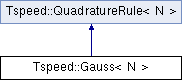
\includegraphics[height=2.000000cm]{classTspeed_1_1Gauss}
\end{center}
\end{figure}
\subsection*{Public Types}
\begin{DoxyCompactItemize}
\item 
enum \{ \hyperlink{classTspeed_1_1Gauss_a91d11e695996fb9038422fdd0d3065aaa13cac1428f86f136e6ed539e3eba50c1}{nqn2d} = N$\ast$\-N
 \}
\item 
enum \{ \hyperlink{classTspeed_1_1Gauss_a501ad3412838918f9e2301655f64eafeadbbfd28e9b0adcf7dfae2dd2b344ff62}{nqn1d} = N
 \}
\item 
typedef \hyperlink{classTspeed_1_1QuadratureRule}{Quadrature\-Rule}$<$ N $>$\-::\hyperlink{classTspeed_1_1QuadratureRule_a195c2b71ad957c9dc5408452b11e1302}{Vec} \hyperlink{classTspeed_1_1Gauss_aa7e6ce3b329db121166dc94669eeb64c}{Vec}
\item 
typedef \hyperlink{classTspeed_1_1QuadratureRule}{Quadrature\-Rule}$<$ N $>$\-::\hyperlink{classTspeed_1_1QuadratureRule_a195c2b71ad957c9dc5408452b11e1302}{Vec} \hyperlink{classTspeed_1_1Gauss_a60a04af13bc0e53cfae47226d1d3e6c2}{Mat}
\item 
typedef \hyperlink{classTspeed_1_1QuadratureRule}{Quadrature\-Rule}$<$ N $>$\-::\hyperlink{classTspeed_1_1QuadratureRule_a195c2b71ad957c9dc5408452b11e1302}{Vec} \hyperlink{classTspeed_1_1Gauss_ae0f9176585d652260498c0b142b183eb}{Vec2}
\end{DoxyCompactItemize}
\subsection*{Public Member Functions}
\begin{DoxyCompactItemize}
\item 
\hyperlink{classTspeed_1_1Gauss_a0bcffd5c12cefd767a96a597c3c250ce}{Gauss} ()
\end{DoxyCompactItemize}
\subsection*{Additional Inherited Members}


\subsection{Detailed Description}
\subsubsection*{template$<$int N$>$class Tspeed\-::\-Gauss$<$ N $>$}

\hyperlink{classTspeed_1_1Gauss}{Gauss} quadrature rule on the triangle. 


\begin{DoxyTemplParams}{Template Parameters}
{\em N} & the order of the rule\\
\hline
\end{DoxyTemplParams}
The internal nodes will be N$^\wedge$2; N+1 is the required order to integrate polynomials of order 2\-N. 

\subsection{Member Typedef Documentation}
\hypertarget{classTspeed_1_1Gauss_a60a04af13bc0e53cfae47226d1d3e6c2}{\index{Tspeed\-::\-Gauss@{Tspeed\-::\-Gauss}!Mat@{Mat}}
\index{Mat@{Mat}!Tspeed::Gauss@{Tspeed\-::\-Gauss}}
\subsubsection[{Mat}]{\setlength{\rightskip}{0pt plus 5cm}template$<$int N$>$ typedef {\bf Quadrature\-Rule}$<$N$>$\-::{\bf Vec} {\bf Tspeed\-::\-Gauss}$<$ N $>$\-::{\bf Mat}}}\label{classTspeed_1_1Gauss_a60a04af13bc0e53cfae47226d1d3e6c2}
\hypertarget{classTspeed_1_1Gauss_aa7e6ce3b329db121166dc94669eeb64c}{\index{Tspeed\-::\-Gauss@{Tspeed\-::\-Gauss}!Vec@{Vec}}
\index{Vec@{Vec}!Tspeed::Gauss@{Tspeed\-::\-Gauss}}
\subsubsection[{Vec}]{\setlength{\rightskip}{0pt plus 5cm}template$<$int N$>$ typedef {\bf Quadrature\-Rule}$<$N$>$\-::{\bf Vec} {\bf Tspeed\-::\-Gauss}$<$ N $>$\-::{\bf Vec}}}\label{classTspeed_1_1Gauss_aa7e6ce3b329db121166dc94669eeb64c}
\hypertarget{classTspeed_1_1Gauss_ae0f9176585d652260498c0b142b183eb}{\index{Tspeed\-::\-Gauss@{Tspeed\-::\-Gauss}!Vec2@{Vec2}}
\index{Vec2@{Vec2}!Tspeed::Gauss@{Tspeed\-::\-Gauss}}
\subsubsection[{Vec2}]{\setlength{\rightskip}{0pt plus 5cm}template$<$int N$>$ typedef {\bf Quadrature\-Rule}$<$N$>$\-::{\bf Vec} {\bf Tspeed\-::\-Gauss}$<$ N $>$\-::{\bf Vec2}}}\label{classTspeed_1_1Gauss_ae0f9176585d652260498c0b142b183eb}


\subsection{Member Enumeration Documentation}
\hypertarget{classTspeed_1_1Gauss_a91d11e695996fb9038422fdd0d3065aa}{\subsubsection[{anonymous enum}]{\setlength{\rightskip}{0pt plus 5cm}template$<$int N$>$ anonymous enum}}\label{classTspeed_1_1Gauss_a91d11e695996fb9038422fdd0d3065aa}
\begin{Desc}
\item[Enumerator]\par
\begin{description}
\index{nqn2d@{nqn2d}!Tspeed\-::\-Gauss@{Tspeed\-::\-Gauss}}\index{Tspeed\-::\-Gauss@{Tspeed\-::\-Gauss}!nqn2d@{nqn2d}}\item[{\em 
\hypertarget{classTspeed_1_1Gauss_a91d11e695996fb9038422fdd0d3065aaa13cac1428f86f136e6ed539e3eba50c1}{nqn2d}\label{classTspeed_1_1Gauss_a91d11e695996fb9038422fdd0d3065aaa13cac1428f86f136e6ed539e3eba50c1}
}]\end{description}
\end{Desc}
\hypertarget{classTspeed_1_1Gauss_a501ad3412838918f9e2301655f64eafe}{\subsubsection[{anonymous enum}]{\setlength{\rightskip}{0pt plus 5cm}template$<$int N$>$ anonymous enum}}\label{classTspeed_1_1Gauss_a501ad3412838918f9e2301655f64eafe}
\begin{Desc}
\item[Enumerator]\par
\begin{description}
\index{nqn1d@{nqn1d}!Tspeed\-::\-Gauss@{Tspeed\-::\-Gauss}}\index{Tspeed\-::\-Gauss@{Tspeed\-::\-Gauss}!nqn1d@{nqn1d}}\item[{\em 
\hypertarget{classTspeed_1_1Gauss_a501ad3412838918f9e2301655f64eafeadbbfd28e9b0adcf7dfae2dd2b344ff62}{nqn1d}\label{classTspeed_1_1Gauss_a501ad3412838918f9e2301655f64eafeadbbfd28e9b0adcf7dfae2dd2b344ff62}
}]\end{description}
\end{Desc}


\subsection{Constructor \& Destructor Documentation}
\hypertarget{classTspeed_1_1Gauss_a0bcffd5c12cefd767a96a597c3c250ce}{\index{Tspeed\-::\-Gauss@{Tspeed\-::\-Gauss}!Gauss@{Gauss}}
\index{Gauss@{Gauss}!Tspeed::Gauss@{Tspeed\-::\-Gauss}}
\subsubsection[{Gauss}]{\setlength{\rightskip}{0pt plus 5cm}template$<$int N$>$ {\bf Tspeed\-::\-Gauss}$<$ N $>$\-::{\bf Gauss} (
\begin{DoxyParamCaption}
{}
\end{DoxyParamCaption}
)}}\label{classTspeed_1_1Gauss_a0bcffd5c12cefd767a96a597c3c250ce}


The documentation for this class was generated from the following files\-:\begin{DoxyCompactItemize}
\item 
lib/include/\hyperlink{QuadratureRule_8hpp}{Quadrature\-Rule.\-hpp}\item 
lib/include/\hyperlink{QuadratureRule__imp_8hpp}{Quadrature\-Rule\-\_\-imp.\-hpp}\end{DoxyCompactItemize}

\hypertarget{classTspeed_1_1LeapFrog}{\section{Tspeed\-:\-:Leap\-Frog Class Reference}
\label{classTspeed_1_1LeapFrog}\index{Tspeed\-::\-Leap\-Frog@{Tspeed\-::\-Leap\-Frog}}
}


Implementation of the second order Leap-\/\-Frog explicit time stepping scheme.  




{\ttfamily \#include $<$Time\-Advance.\-hpp$>$}

Inheritance diagram for Tspeed\-:\-:Leap\-Frog\-:\begin{figure}[H]
\begin{center}
\leavevmode
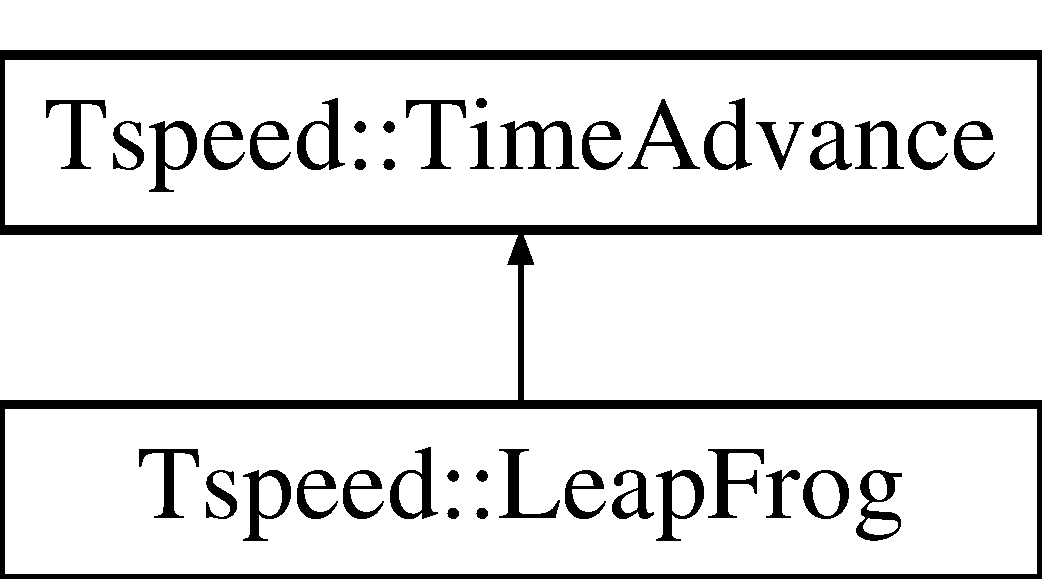
\includegraphics[height=2.000000cm]{classTspeed_1_1LeapFrog}
\end{center}
\end{figure}
\subsection*{Public Member Functions}
\begin{DoxyCompactItemize}
\item 
{\footnotesize template$<$int N, typename Q , typename S $>$ }\\\hyperlink{classTspeed_1_1LeapFrog_a444fa2e71465a70a4be750395d4e6908}{Leap\-Frog} (\hyperlink{namespaceTspeed_a05fcb57094666c8f5ab1e90d1a6fecf8}{F\-E\-Space\-\_\-ptr}$<$ N, Q, S $>$, \hyperlink{classTspeed_1_1Parameters}{Parameters} const \&, \hyperlink{classTspeed_1_1Receivers}{Receivers} const \&)
\item 
void \hyperlink{classTspeed_1_1LeapFrog_aad6f9246550ac8dda3d8b00fc713604b}{first\-\_\-step} ()
\begin{DoxyCompactList}\small\item\em First step for the Leap-\/\-Frog method. \end{DoxyCompactList}\item 
void \hyperlink{classTspeed_1_1LeapFrog_a571d3a80ef86424a14b562295aaae52e}{step} (double)
\begin{DoxyCompactList}\small\item\em Step at time t for the Leap-\/\-Frog method. \end{DoxyCompactList}\end{DoxyCompactItemize}
\subsection*{Additional Inherited Members}


\subsection{Detailed Description}
Implementation of the second order Leap-\/\-Frog explicit time stepping scheme. 

\subsection{Constructor \& Destructor Documentation}
\hypertarget{classTspeed_1_1LeapFrog_a444fa2e71465a70a4be750395d4e6908}{\index{Tspeed\-::\-Leap\-Frog@{Tspeed\-::\-Leap\-Frog}!Leap\-Frog@{Leap\-Frog}}
\index{Leap\-Frog@{Leap\-Frog}!Tspeed::LeapFrog@{Tspeed\-::\-Leap\-Frog}}
\subsubsection[{Leap\-Frog}]{\setlength{\rightskip}{0pt plus 5cm}template$<$int N, typename Q , typename S $>$ Tspeed\-::\-Leap\-Frog\-::\-Leap\-Frog (
\begin{DoxyParamCaption}
\item[{{\bf F\-E\-Space\-\_\-ptr}$<$ N, Q, S $>$}]{Xh, }
\item[{{\bf Parameters} const \&}]{p, }
\item[{{\bf Receivers} const \&}]{r}
\end{DoxyParamCaption}
)}}\label{classTspeed_1_1LeapFrog_a444fa2e71465a70a4be750395d4e6908}


\subsection{Member Function Documentation}
\hypertarget{classTspeed_1_1LeapFrog_aad6f9246550ac8dda3d8b00fc713604b}{\index{Tspeed\-::\-Leap\-Frog@{Tspeed\-::\-Leap\-Frog}!first\-\_\-step@{first\-\_\-step}}
\index{first\-\_\-step@{first\-\_\-step}!Tspeed::LeapFrog@{Tspeed\-::\-Leap\-Frog}}
\subsubsection[{first\-\_\-step}]{\setlength{\rightskip}{0pt plus 5cm}void Tspeed\-::\-Leap\-Frog\-::first\-\_\-step (
\begin{DoxyParamCaption}
{}
\end{DoxyParamCaption}
)}}\label{classTspeed_1_1LeapFrog_aad6f9246550ac8dda3d8b00fc713604b}


First step for the Leap-\/\-Frog method. 

\hypertarget{classTspeed_1_1LeapFrog_a571d3a80ef86424a14b562295aaae52e}{\index{Tspeed\-::\-Leap\-Frog@{Tspeed\-::\-Leap\-Frog}!step@{step}}
\index{step@{step}!Tspeed::LeapFrog@{Tspeed\-::\-Leap\-Frog}}
\subsubsection[{step}]{\setlength{\rightskip}{0pt plus 5cm}void Tspeed\-::\-Leap\-Frog\-::step (
\begin{DoxyParamCaption}
\item[{double}]{t}
\end{DoxyParamCaption}
)}}\label{classTspeed_1_1LeapFrog_a571d3a80ef86424a14b562295aaae52e}


Step at time t for the Leap-\/\-Frog method. 


\begin{DoxyParams}{Parameters}
{\em t} & time \\
\hline
\end{DoxyParams}


The documentation for this class was generated from the following files\-:\begin{DoxyCompactItemize}
\item 
lib/include/\hyperlink{TimeAdvance_8hpp}{Time\-Advance.\-hpp}\item 
lib/include/\hyperlink{TimeAdvance__imp_8hpp}{Time\-Advance\-\_\-imp.\-hpp}\item 
lib/src/\hyperlink{TimeAdvance_8cpp}{Time\-Advance.\-cpp}\end{DoxyCompactItemize}

\hypertarget{classTspeed_1_1Matrices}{\section{Tspeed\-:\-:Matrices Class Reference}
\label{classTspeed_1_1Matrices}\index{Tspeed\-::\-Matrices@{Tspeed\-::\-Matrices}}
}


{\ttfamily \#include $<$Time\-Advance.\-hpp$>$}

\subsection*{Public Types}
\begin{DoxyCompactItemize}
\item 
typedef Eigen\-::\-Sparse\-Matrix\\*
$<$ double $>$ \hyperlink{classTspeed_1_1Matrices_aec4249f1ac32c3249adae9c91bac1cbf}{Sp\-Mat}
\end{DoxyCompactItemize}
\subsection*{Public Member Functions}
\begin{DoxyCompactItemize}
\item 
{\footnotesize template$<$int N, typename Q , typename S $>$ }\\\hyperlink{classTspeed_1_1Matrices_ad4b46e2f7a2056a6c5f3a803157236bc}{Matrices} (\hyperlink{namespaceTspeed_a05fcb57094666c8f5ab1e90d1a6fecf8}{F\-E\-Space\-\_\-ptr}$<$ N, Q, S $>$, \hyperlink{classTspeed_1_1Parameters}{Parameters} const \&)
\item 
\hyperlink{classTspeed_1_1MyMatMultiDim}{My\-Mat\-Multi\-Dim}$<$ \hyperlink{classTspeed_1_1MyMatBlockDiag}{My\-Mat\-Block\-Diag} $>$\\*
 const \& \hyperlink{classTspeed_1_1Matrices_a4ee3310af2c6fa476099673ebf61c242}{get\-A} ()
\item 
\hyperlink{classTspeed_1_1MyMatMultiDim}{My\-Mat\-Multi\-Dim}$<$ \hyperlink{classTspeed_1_1MyMat}{My\-Mat} $>$ const \& \hyperlink{classTspeed_1_1Matrices_a95dfd802f178cf5dc51967ad70cf36cd}{get\-S} ()
\item 
\hyperlink{classTspeed_1_1MyMatMultiDim}{My\-Mat\-Multi\-Dim}$<$ \hyperlink{classTspeed_1_1MyMat}{My\-Mat} $>$ const \& \hyperlink{classTspeed_1_1Matrices_a78c435049af0aa48eacd9a9dc99627fa}{get\-I} ()
\item 
\hyperlink{classTspeed_1_1MyMatMultiDimBlockDiag}{My\-Mat\-Multi\-Dim\-Block\-Diag}\\*
$<$ \hyperlink{classTspeed_1_1MyMatBlockDiag}{My\-Mat\-Block\-Diag} $>$ const \& \hyperlink{classTspeed_1_1Matrices_a5358482d27d03d838c597ec2eb79a71c}{getinv\-M} ()
\item 
{\footnotesize template$<$int N, typename Q , typename T $>$ }\\\hyperlink{classTspeed_1_1Matrices_a1893bd97b0320d078e6cd1e97e3cbd5a}{Matrices} (\hyperlink{namespaceTspeed_a05fcb57094666c8f5ab1e90d1a6fecf8}{F\-E\-Space\-\_\-ptr}$<$ N, Q, T $>$ Xh, \hyperlink{classTspeed_1_1Parameters}{Parameters} const \&P)
\end{DoxyCompactItemize}


\subsection{Member Typedef Documentation}
\hypertarget{classTspeed_1_1Matrices_aec4249f1ac32c3249adae9c91bac1cbf}{\index{Tspeed\-::\-Matrices@{Tspeed\-::\-Matrices}!Sp\-Mat@{Sp\-Mat}}
\index{Sp\-Mat@{Sp\-Mat}!Tspeed::Matrices@{Tspeed\-::\-Matrices}}
\subsubsection[{Sp\-Mat}]{\setlength{\rightskip}{0pt plus 5cm}typedef Eigen\-::\-Sparse\-Matrix$<$double$>$ {\bf Tspeed\-::\-Matrices\-::\-Sp\-Mat}}}\label{classTspeed_1_1Matrices_aec4249f1ac32c3249adae9c91bac1cbf}


\subsection{Constructor \& Destructor Documentation}
\hypertarget{classTspeed_1_1Matrices_ad4b46e2f7a2056a6c5f3a803157236bc}{\index{Tspeed\-::\-Matrices@{Tspeed\-::\-Matrices}!Matrices@{Matrices}}
\index{Matrices@{Matrices}!Tspeed::Matrices@{Tspeed\-::\-Matrices}}
\subsubsection[{Matrices}]{\setlength{\rightskip}{0pt plus 5cm}template$<$int N, typename Q , typename S $>$ Tspeed\-::\-Matrices\-::\-Matrices (
\begin{DoxyParamCaption}
\item[{{\bf F\-E\-Space\-\_\-ptr}$<$ N, Q, S $>$}]{, }
\item[{{\bf Parameters} const \&}]{}
\end{DoxyParamCaption}
)}}\label{classTspeed_1_1Matrices_ad4b46e2f7a2056a6c5f3a803157236bc}
\hypertarget{classTspeed_1_1Matrices_a1893bd97b0320d078e6cd1e97e3cbd5a}{\index{Tspeed\-::\-Matrices@{Tspeed\-::\-Matrices}!Matrices@{Matrices}}
\index{Matrices@{Matrices}!Tspeed::Matrices@{Tspeed\-::\-Matrices}}
\subsubsection[{Matrices}]{\setlength{\rightskip}{0pt plus 5cm}template$<$int N, typename Q , typename T $>$ Tspeed\-::\-Matrices\-::\-Matrices (
\begin{DoxyParamCaption}
\item[{{\bf F\-E\-Space\-\_\-ptr}$<$ N, Q, T $>$}]{Xh, }
\item[{{\bf Parameters} const \&}]{P}
\end{DoxyParamCaption}
)}}\label{classTspeed_1_1Matrices_a1893bd97b0320d078e6cd1e97e3cbd5a}


\subsection{Member Function Documentation}
\hypertarget{classTspeed_1_1Matrices_a4ee3310af2c6fa476099673ebf61c242}{\index{Tspeed\-::\-Matrices@{Tspeed\-::\-Matrices}!get\-A@{get\-A}}
\index{get\-A@{get\-A}!Tspeed::Matrices@{Tspeed\-::\-Matrices}}
\subsubsection[{get\-A}]{\setlength{\rightskip}{0pt plus 5cm}{\bf My\-Mat\-Multi\-Dim}$<${\bf My\-Mat\-Block\-Diag}$>$ const\& Tspeed\-::\-Matrices\-::get\-A (
\begin{DoxyParamCaption}
{}
\end{DoxyParamCaption}
)\hspace{0.3cm}{\ttfamily [inline]}}}\label{classTspeed_1_1Matrices_a4ee3310af2c6fa476099673ebf61c242}
\hypertarget{classTspeed_1_1Matrices_a78c435049af0aa48eacd9a9dc99627fa}{\index{Tspeed\-::\-Matrices@{Tspeed\-::\-Matrices}!get\-I@{get\-I}}
\index{get\-I@{get\-I}!Tspeed::Matrices@{Tspeed\-::\-Matrices}}
\subsubsection[{get\-I}]{\setlength{\rightskip}{0pt plus 5cm}{\bf My\-Mat\-Multi\-Dim}$<${\bf My\-Mat}$>$ const\& Tspeed\-::\-Matrices\-::get\-I (
\begin{DoxyParamCaption}
{}
\end{DoxyParamCaption}
)\hspace{0.3cm}{\ttfamily [inline]}}}\label{classTspeed_1_1Matrices_a78c435049af0aa48eacd9a9dc99627fa}
\hypertarget{classTspeed_1_1Matrices_a5358482d27d03d838c597ec2eb79a71c}{\index{Tspeed\-::\-Matrices@{Tspeed\-::\-Matrices}!getinv\-M@{getinv\-M}}
\index{getinv\-M@{getinv\-M}!Tspeed::Matrices@{Tspeed\-::\-Matrices}}
\subsubsection[{getinv\-M}]{\setlength{\rightskip}{0pt plus 5cm}{\bf My\-Mat\-Multi\-Dim\-Block\-Diag}$<${\bf My\-Mat\-Block\-Diag}$>$ const\& Tspeed\-::\-Matrices\-::getinv\-M (
\begin{DoxyParamCaption}
{}
\end{DoxyParamCaption}
)\hspace{0.3cm}{\ttfamily [inline]}}}\label{classTspeed_1_1Matrices_a5358482d27d03d838c597ec2eb79a71c}
\hypertarget{classTspeed_1_1Matrices_a95dfd802f178cf5dc51967ad70cf36cd}{\index{Tspeed\-::\-Matrices@{Tspeed\-::\-Matrices}!get\-S@{get\-S}}
\index{get\-S@{get\-S}!Tspeed::Matrices@{Tspeed\-::\-Matrices}}
\subsubsection[{get\-S}]{\setlength{\rightskip}{0pt plus 5cm}{\bf My\-Mat\-Multi\-Dim}$<${\bf My\-Mat}$>$ const\& Tspeed\-::\-Matrices\-::get\-S (
\begin{DoxyParamCaption}
{}
\end{DoxyParamCaption}
)\hspace{0.3cm}{\ttfamily [inline]}}}\label{classTspeed_1_1Matrices_a95dfd802f178cf5dc51967ad70cf36cd}


The documentation for this class was generated from the following files\-:\begin{DoxyCompactItemize}
\item 
lib/include/\hyperlink{TimeAdvance_8hpp}{Time\-Advance.\-hpp}\item 
lib/include/\hyperlink{Matrices__imp_8hpp}{Matrices\-\_\-imp.\-hpp}\end{DoxyCompactItemize}

\hypertarget{classTspeed_1_1Mesh}{\section{Tspeed\-:\-:Mesh Class Reference}
\label{classTspeed_1_1Mesh}\index{Tspeed\-::\-Mesh@{Tspeed\-::\-Mesh}}
}


{\ttfamily \#include $<$Mesh.\-hpp$>$}

\subsection*{Public Types}
\begin{DoxyCompactItemize}
\item 
typedef unsigned int \hyperlink{classTspeed_1_1Mesh_a097181c50faa6c8cec5dbe135694606b}{size\-\_\-type}
\item 
typedef std\-::vector\\*
$<$ \hyperlink{classTspeed_1_1Geo_1_1Triangle}{Geo\-::\-Triangle}, \\*
Eigen\-::aligned\-\_\-allocator\\*
$<$ Eigen\-::\-Vector2d $>$ $>$ \hyperlink{classTspeed_1_1Mesh_ae62a59eea301689dd9f7c9663414db18}{Aligned\-Vec\-T}
\item 
typedef std\-::vector$<$ \hyperlink{classTspeed_1_1Geo_1_1Edge}{Geo\-::\-Edge}, \\*
Eigen\-::aligned\-\_\-allocator\\*
$<$ Eigen\-::\-Vector2d $>$ $>$ \hyperlink{classTspeed_1_1Mesh_a09031b0dab0f2efcef61981dfc9d1640}{Aligned\-Vec\-E}
\item 
typedef std\-::vector\\*
$<$ \hyperlink{classTspeed_1_1Geo_1_1Point}{Geo\-::\-Point}, \\*
Eigen\-::aligned\-\_\-allocator\\*
$<$ Eigen\-::\-Vector2d $>$ $>$ \hyperlink{classTspeed_1_1Mesh_aa8aac31131166087d192ef77c49fb5b2}{Aligned\-Vec\-P}
\end{DoxyCompactItemize}
\subsection*{Public Member Functions}
\begin{DoxyCompactItemize}
\item 
\hyperlink{classTspeed_1_1Mesh_a2359bc61d5acea3515e31b5b3a9d1edf}{Mesh} (const std\-::string file\-Name)
\begin{DoxyCompactList}\small\item\em Generate mesh from a Gmsh mesh. \end{DoxyCompactList}\item 
\hyperlink{classTspeed_1_1Geo_1_1Triangle}{Geo\-::\-Triangle} const \& \hyperlink{classTspeed_1_1Mesh_a20ac8fd5940e93ec902f343211100d78}{operator\mbox{[}$\,$\mbox{]}} (size\-\_\-t i) const 
\begin{DoxyCompactList}\small\item\em Get triangle with index i (const) \end{DoxyCompactList}\item 
\hyperlink{classTspeed_1_1Geo_1_1Triangle}{Geo\-::\-Triangle} \& \hyperlink{classTspeed_1_1Mesh_af6688d1a47cee1baf69ea6d38d721a4a}{operator\mbox{[}$\,$\mbox{]}} (size\-\_\-t i)
\begin{DoxyCompactList}\small\item\em Get triangle with index i ( non-\/const) \end{DoxyCompactList}\item 
\hyperlink{classTspeed_1_1Mesh_ae62a59eea301689dd9f7c9663414db18}{Aligned\-Vec\-T} const \& \hyperlink{classTspeed_1_1Mesh_ac889d7a89a2d98e84dbc9f0f1b2ebb45}{elements} () const 
\begin{DoxyCompactList}\small\item\em Get all triangles in the mesh (const) \end{DoxyCompactList}\item 
\hyperlink{classTspeed_1_1Mesh_ae62a59eea301689dd9f7c9663414db18}{Aligned\-Vec\-T} \& \hyperlink{classTspeed_1_1Mesh_a0e9102ce786fc8c4cda93c4b012c8668}{elements} ()
\begin{DoxyCompactList}\small\item\em Get all triangles in the mesh (non-\/const) \end{DoxyCompactList}\item 
\hyperlink{classTspeed_1_1Mesh_ae4422add9d3952fe2c02f62053ec120f}{$\sim$\-Mesh} ()
\item 
void \hyperlink{classTspeed_1_1Mesh_a10b24b91186b9905847232e7e14d4b2e}{stats} () const 
\begin{DoxyCompactList}\small\item\em Print stats about the mesh (e.\-g. number of elements, anisotropy etc.) \end{DoxyCompactList}\item 
unsigned int \hyperlink{classTspeed_1_1Mesh_ac5b8a388b633ac0d280f89f56f2b15c5}{ne} () const 
\begin{DoxyCompactList}\small\item\em Get number of triangles in the mesh. \end{DoxyCompactList}\item 
void \hyperlink{classTspeed_1_1Mesh_a7ea0757951214e8dc3a68e9a60a1c17c}{printall\-Neigh} () const 
\begin{DoxyCompactList}\small\item\em Print neighbors structure. \end{DoxyCompactList}\end{DoxyCompactItemize}
\subsection*{Public Attributes}
\begin{DoxyCompactItemize}
\item 
std\-::vector$<$ std\-::pair\\*
$<$ unsigned int, unsigned int $>$ $>$ \hyperlink{classTspeed_1_1Mesh_a8cb823f02d7c75e48bf714b367b25b7d}{M\-\_\-bed\-\_\-map}
\end{DoxyCompactItemize}


\subsection{Member Typedef Documentation}
\hypertarget{classTspeed_1_1Mesh_a09031b0dab0f2efcef61981dfc9d1640}{\index{Tspeed\-::\-Mesh@{Tspeed\-::\-Mesh}!Aligned\-Vec\-E@{Aligned\-Vec\-E}}
\index{Aligned\-Vec\-E@{Aligned\-Vec\-E}!Tspeed::Mesh@{Tspeed\-::\-Mesh}}
\subsubsection[{Aligned\-Vec\-E}]{\setlength{\rightskip}{0pt plus 5cm}typedef std\-::vector$<${\bf Geo\-::\-Edge},Eigen\-::aligned\-\_\-allocator$<$Eigen\-::\-Vector2d$>$ $>$ {\bf Tspeed\-::\-Mesh\-::\-Aligned\-Vec\-E}}}\label{classTspeed_1_1Mesh_a09031b0dab0f2efcef61981dfc9d1640}
\hypertarget{classTspeed_1_1Mesh_aa8aac31131166087d192ef77c49fb5b2}{\index{Tspeed\-::\-Mesh@{Tspeed\-::\-Mesh}!Aligned\-Vec\-P@{Aligned\-Vec\-P}}
\index{Aligned\-Vec\-P@{Aligned\-Vec\-P}!Tspeed::Mesh@{Tspeed\-::\-Mesh}}
\subsubsection[{Aligned\-Vec\-P}]{\setlength{\rightskip}{0pt plus 5cm}typedef std\-::vector$<${\bf Geo\-::\-Point},Eigen\-::aligned\-\_\-allocator$<$Eigen\-::\-Vector2d$>$ $>$ {\bf Tspeed\-::\-Mesh\-::\-Aligned\-Vec\-P}}}\label{classTspeed_1_1Mesh_aa8aac31131166087d192ef77c49fb5b2}
\hypertarget{classTspeed_1_1Mesh_ae62a59eea301689dd9f7c9663414db18}{\index{Tspeed\-::\-Mesh@{Tspeed\-::\-Mesh}!Aligned\-Vec\-T@{Aligned\-Vec\-T}}
\index{Aligned\-Vec\-T@{Aligned\-Vec\-T}!Tspeed::Mesh@{Tspeed\-::\-Mesh}}
\subsubsection[{Aligned\-Vec\-T}]{\setlength{\rightskip}{0pt plus 5cm}typedef std\-::vector$<${\bf Geo\-::\-Triangle},Eigen\-::aligned\-\_\-allocator$<$Eigen\-::\-Vector2d$>$ $>$ {\bf Tspeed\-::\-Mesh\-::\-Aligned\-Vec\-T}}}\label{classTspeed_1_1Mesh_ae62a59eea301689dd9f7c9663414db18}
\hypertarget{classTspeed_1_1Mesh_a097181c50faa6c8cec5dbe135694606b}{\index{Tspeed\-::\-Mesh@{Tspeed\-::\-Mesh}!size\-\_\-type@{size\-\_\-type}}
\index{size\-\_\-type@{size\-\_\-type}!Tspeed::Mesh@{Tspeed\-::\-Mesh}}
\subsubsection[{size\-\_\-type}]{\setlength{\rightskip}{0pt plus 5cm}typedef unsigned int {\bf Tspeed\-::\-Mesh\-::size\-\_\-type}}}\label{classTspeed_1_1Mesh_a097181c50faa6c8cec5dbe135694606b}


\subsection{Constructor \& Destructor Documentation}
\hypertarget{classTspeed_1_1Mesh_a2359bc61d5acea3515e31b5b3a9d1edf}{\index{Tspeed\-::\-Mesh@{Tspeed\-::\-Mesh}!Mesh@{Mesh}}
\index{Mesh@{Mesh}!Tspeed::Mesh@{Tspeed\-::\-Mesh}}
\subsubsection[{Mesh}]{\setlength{\rightskip}{0pt plus 5cm}Tspeed\-::\-Mesh\-::\-Mesh (
\begin{DoxyParamCaption}
\item[{const std\-::string}]{file\-Name}
\end{DoxyParamCaption}
)\hspace{0.3cm}{\ttfamily [explicit]}}}\label{classTspeed_1_1Mesh_a2359bc61d5acea3515e31b5b3a9d1edf}


Generate mesh from a Gmsh mesh. 


\begin{DoxyParams}{Parameters}
{\em file\-Name} & Name of the .msh file containing the mesh \\
\hline
\end{DoxyParams}
\hypertarget{classTspeed_1_1Mesh_ae4422add9d3952fe2c02f62053ec120f}{\index{Tspeed\-::\-Mesh@{Tspeed\-::\-Mesh}!$\sim$\-Mesh@{$\sim$\-Mesh}}
\index{$\sim$\-Mesh@{$\sim$\-Mesh}!Tspeed::Mesh@{Tspeed\-::\-Mesh}}
\subsubsection[{$\sim$\-Mesh}]{\setlength{\rightskip}{0pt plus 5cm}Tspeed\-::\-Mesh\-::$\sim$\-Mesh (
\begin{DoxyParamCaption}
{}
\end{DoxyParamCaption}
)\hspace{0.3cm}{\ttfamily [inline]}}}\label{classTspeed_1_1Mesh_ae4422add9d3952fe2c02f62053ec120f}


\subsection{Member Function Documentation}
\hypertarget{classTspeed_1_1Mesh_ac889d7a89a2d98e84dbc9f0f1b2ebb45}{\index{Tspeed\-::\-Mesh@{Tspeed\-::\-Mesh}!elements@{elements}}
\index{elements@{elements}!Tspeed::Mesh@{Tspeed\-::\-Mesh}}
\subsubsection[{elements}]{\setlength{\rightskip}{0pt plus 5cm}{\bf Aligned\-Vec\-T} const\& Tspeed\-::\-Mesh\-::elements (
\begin{DoxyParamCaption}
{}
\end{DoxyParamCaption}
) const\hspace{0.3cm}{\ttfamily [inline]}}}\label{classTspeed_1_1Mesh_ac889d7a89a2d98e84dbc9f0f1b2ebb45}


Get all triangles in the mesh (const) 

\begin{DoxyReturn}{Returns}
Constant reference to a vector of triangles 
\end{DoxyReturn}
\hypertarget{classTspeed_1_1Mesh_a0e9102ce786fc8c4cda93c4b012c8668}{\index{Tspeed\-::\-Mesh@{Tspeed\-::\-Mesh}!elements@{elements}}
\index{elements@{elements}!Tspeed::Mesh@{Tspeed\-::\-Mesh}}
\subsubsection[{elements}]{\setlength{\rightskip}{0pt plus 5cm}{\bf Aligned\-Vec\-T}\& Tspeed\-::\-Mesh\-::elements (
\begin{DoxyParamCaption}
{}
\end{DoxyParamCaption}
)\hspace{0.3cm}{\ttfamily [inline]}}}\label{classTspeed_1_1Mesh_a0e9102ce786fc8c4cda93c4b012c8668}


Get all triangles in the mesh (non-\/const) 

\begin{DoxyReturn}{Returns}
Reference to a vector of triangles 
\end{DoxyReturn}
\hypertarget{classTspeed_1_1Mesh_ac5b8a388b633ac0d280f89f56f2b15c5}{\index{Tspeed\-::\-Mesh@{Tspeed\-::\-Mesh}!ne@{ne}}
\index{ne@{ne}!Tspeed::Mesh@{Tspeed\-::\-Mesh}}
\subsubsection[{ne}]{\setlength{\rightskip}{0pt plus 5cm}unsigned int Tspeed\-::\-Mesh\-::ne (
\begin{DoxyParamCaption}
{}
\end{DoxyParamCaption}
) const\hspace{0.3cm}{\ttfamily [inline]}}}\label{classTspeed_1_1Mesh_ac5b8a388b633ac0d280f89f56f2b15c5}


Get number of triangles in the mesh. 

\hypertarget{classTspeed_1_1Mesh_a20ac8fd5940e93ec902f343211100d78}{\index{Tspeed\-::\-Mesh@{Tspeed\-::\-Mesh}!operator\mbox{[}$\,$\mbox{]}@{operator[]}}
\index{operator\mbox{[}$\,$\mbox{]}@{operator[]}!Tspeed::Mesh@{Tspeed\-::\-Mesh}}
\subsubsection[{operator[]}]{\setlength{\rightskip}{0pt plus 5cm}{\bf Geo\-::\-Triangle} const\& Tspeed\-::\-Mesh\-::operator\mbox{[}$\,$\mbox{]} (
\begin{DoxyParamCaption}
\item[{size\-\_\-t}]{i}
\end{DoxyParamCaption}
) const\hspace{0.3cm}{\ttfamily [inline]}}}\label{classTspeed_1_1Mesh_a20ac8fd5940e93ec902f343211100d78}


Get triangle with index i (const) 


\begin{DoxyParams}{Parameters}
{\em i} & index of the triangle\\
\hline
\end{DoxyParams}
\begin{DoxyReturn}{Returns}
Constant reference to triangle 
\end{DoxyReturn}
\hypertarget{classTspeed_1_1Mesh_af6688d1a47cee1baf69ea6d38d721a4a}{\index{Tspeed\-::\-Mesh@{Tspeed\-::\-Mesh}!operator\mbox{[}$\,$\mbox{]}@{operator[]}}
\index{operator\mbox{[}$\,$\mbox{]}@{operator[]}!Tspeed::Mesh@{Tspeed\-::\-Mesh}}
\subsubsection[{operator[]}]{\setlength{\rightskip}{0pt plus 5cm}{\bf Geo\-::\-Triangle}\& Tspeed\-::\-Mesh\-::operator\mbox{[}$\,$\mbox{]} (
\begin{DoxyParamCaption}
\item[{size\-\_\-t}]{i}
\end{DoxyParamCaption}
)\hspace{0.3cm}{\ttfamily [inline]}}}\label{classTspeed_1_1Mesh_af6688d1a47cee1baf69ea6d38d721a4a}


Get triangle with index i ( non-\/const) 


\begin{DoxyParams}{Parameters}
{\em i} & index of the triangle\\
\hline
\end{DoxyParams}
\begin{DoxyReturn}{Returns}
Reference to triangle 
\end{DoxyReturn}
\hypertarget{classTspeed_1_1Mesh_a7ea0757951214e8dc3a68e9a60a1c17c}{\index{Tspeed\-::\-Mesh@{Tspeed\-::\-Mesh}!printall\-Neigh@{printall\-Neigh}}
\index{printall\-Neigh@{printall\-Neigh}!Tspeed::Mesh@{Tspeed\-::\-Mesh}}
\subsubsection[{printall\-Neigh}]{\setlength{\rightskip}{0pt plus 5cm}void Tspeed\-::\-Mesh\-::printall\-Neigh (
\begin{DoxyParamCaption}
{}
\end{DoxyParamCaption}
) const\hspace{0.3cm}{\ttfamily [inline]}}}\label{classTspeed_1_1Mesh_a7ea0757951214e8dc3a68e9a60a1c17c}


Print neighbors structure. 

\hypertarget{classTspeed_1_1Mesh_a10b24b91186b9905847232e7e14d4b2e}{\index{Tspeed\-::\-Mesh@{Tspeed\-::\-Mesh}!stats@{stats}}
\index{stats@{stats}!Tspeed::Mesh@{Tspeed\-::\-Mesh}}
\subsubsection[{stats}]{\setlength{\rightskip}{0pt plus 5cm}void Tspeed\-::\-Mesh\-::stats (
\begin{DoxyParamCaption}
{}
\end{DoxyParamCaption}
) const}}\label{classTspeed_1_1Mesh_a10b24b91186b9905847232e7e14d4b2e}


Print stats about the mesh (e.\-g. number of elements, anisotropy etc.) 



\subsection{Member Data Documentation}
\hypertarget{classTspeed_1_1Mesh_a8cb823f02d7c75e48bf714b367b25b7d}{\index{Tspeed\-::\-Mesh@{Tspeed\-::\-Mesh}!M\-\_\-bed\-\_\-map@{M\-\_\-bed\-\_\-map}}
\index{M\-\_\-bed\-\_\-map@{M\-\_\-bed\-\_\-map}!Tspeed::Mesh@{Tspeed\-::\-Mesh}}
\subsubsection[{M\-\_\-bed\-\_\-map}]{\setlength{\rightskip}{0pt plus 5cm}std\-::vector$<$std\-::pair$<$unsigned int,unsigned int$>$ $>$ Tspeed\-::\-Mesh\-::\-M\-\_\-bed\-\_\-map}}\label{classTspeed_1_1Mesh_a8cb823f02d7c75e48bf714b367b25b7d}


The documentation for this class was generated from the following files\-:\begin{DoxyCompactItemize}
\item 
lib/include/\hyperlink{Mesh_8hpp}{Mesh.\-hpp}\item 
lib/src/\hyperlink{Mesh_8cpp}{Mesh.\-cpp}\end{DoxyCompactItemize}

\hypertarget{classTspeed_1_1MyMat}{\section{Tspeed\-:\-:My\-Mat Class Reference}
\label{classTspeed_1_1MyMat}\index{Tspeed\-::\-My\-Mat@{Tspeed\-::\-My\-Mat}}
}


{\ttfamily \#include $<$My\-Mat.\-hpp$>$}

Inheritance diagram for Tspeed\-:\-:My\-Mat\-:\begin{figure}[H]
\begin{center}
\leavevmode
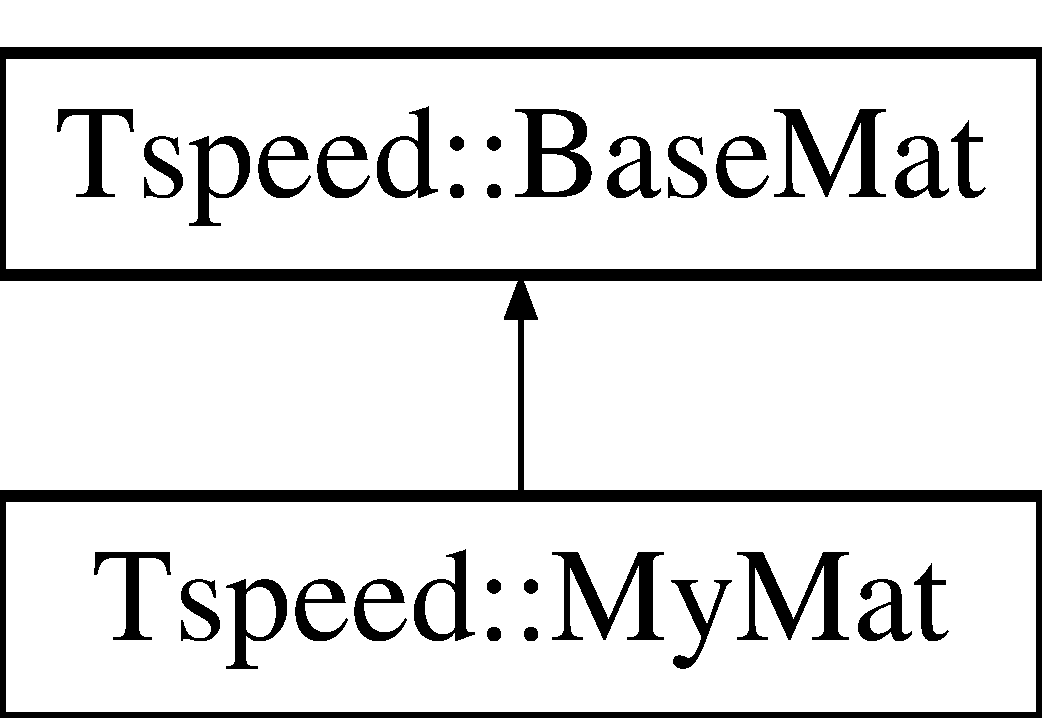
\includegraphics[height=2.000000cm]{classTspeed_1_1MyMat}
\end{center}
\end{figure}
\subsection*{Public Member Functions}
\begin{DoxyCompactItemize}
\item 
\hyperlink{classTspeed_1_1MyMat_a8fbd3586cb4653ea3cdb2b9d42428e85}{My\-Mat} ()
\item 
\hyperlink{classTspeed_1_1MyMat_a4f07d60d8010d796e27fb90c367b1c8a}{My\-Mat} (\hyperlink{namespaceTspeed_a7367a01365c4cc2c1a09305b3effc4e8}{Mesh\-\_\-ptr}, unsigned int nln)
\item 
\hyperlink{classTspeed_1_1MyMat_adc35adc0df81f0be813200c96c294bdc}{My\-Mat} (\hyperlink{classTspeed_1_1MyMat}{My\-Mat} \&\&)=default
\item 
\hyperlink{classTspeed_1_1MyMat_af0996d6425e454b7afb2e5f27c6b77be}{My\-Mat} (\hyperlink{classTspeed_1_1MyMat}{My\-Mat} const \&)
\item 
\hyperlink{classTspeed_1_1MyMat}{My\-Mat} \& \hyperlink{classTspeed_1_1MyMat_a1c595cc39c627f9556f7b2a3548f3da8}{operator=} (\hyperlink{classTspeed_1_1MyMat}{My\-Mat} \&\&)=default
\item 
\hyperlink{classTspeed_1_1MyMat}{My\-Mat} \& \hyperlink{classTspeed_1_1MyMat_ad9a206ca7e833b341c58424e3096641c}{operator=} (\hyperlink{classTspeed_1_1MyMat}{My\-Mat} const \&)=default
\item 
virtual \hyperlink{classTspeed_1_1MyMat_a3b10142286aebdd62af6c38eef9790e5}{$\sim$\-My\-Mat} () noexcept(true)=default
\item 
void \hyperlink{classTspeed_1_1MyMat_a32eb1340d490fc050d6c6f22a0c84a29}{symmetrize} ()
\item 
void \hyperlink{classTspeed_1_1MyMat_a565da9a269ad2afc5fcd1f358550f732}{sumtranspose} (\hyperlink{classTspeed_1_1MyMat}{My\-Mat} const \&)
\item 
\hyperlink{classTspeed_1_1MyMat}{My\-Mat} \hyperlink{classTspeed_1_1MyMat_aa9b048f523b8f2887ce3a2d578cab6b3}{operator+=} (\hyperlink{classTspeed_1_1MyMat}{My\-Mat} const \&)
\item 
\hyperlink{classTspeed_1_1MyMat}{My\-Mat} \hyperlink{classTspeed_1_1MyMat_a523a402aa8afdb2b270413b8796b0b5f}{operator+=} (\hyperlink{classTspeed_1_1MyMatBlockDiag}{My\-Mat\-Block\-Diag} const \&)
\item 
\hyperlink{classTspeed_1_1MyMat}{My\-Mat} \hyperlink{classTspeed_1_1MyMat_a8aa3f178e8723a2ac133e3debe0f4655}{operator$\ast$} (double const \&) const 
\end{DoxyCompactItemize}
\subsection*{Additional Inherited Members}


\subsection{Constructor \& Destructor Documentation}
\hypertarget{classTspeed_1_1MyMat_a8fbd3586cb4653ea3cdb2b9d42428e85}{\index{Tspeed\-::\-My\-Mat@{Tspeed\-::\-My\-Mat}!My\-Mat@{My\-Mat}}
\index{My\-Mat@{My\-Mat}!Tspeed::MyMat@{Tspeed\-::\-My\-Mat}}
\subsubsection[{My\-Mat}]{\setlength{\rightskip}{0pt plus 5cm}Tspeed\-::\-My\-Mat\-::\-My\-Mat (
\begin{DoxyParamCaption}
{}
\end{DoxyParamCaption}
)\hspace{0.3cm}{\ttfamily [inline]}}}\label{classTspeed_1_1MyMat_a8fbd3586cb4653ea3cdb2b9d42428e85}
\hypertarget{classTspeed_1_1MyMat_a4f07d60d8010d796e27fb90c367b1c8a}{\index{Tspeed\-::\-My\-Mat@{Tspeed\-::\-My\-Mat}!My\-Mat@{My\-Mat}}
\index{My\-Mat@{My\-Mat}!Tspeed::MyMat@{Tspeed\-::\-My\-Mat}}
\subsubsection[{My\-Mat}]{\setlength{\rightskip}{0pt plus 5cm}Tspeed\-::\-My\-Mat\-::\-My\-Mat (
\begin{DoxyParamCaption}
\item[{{\bf Mesh\-\_\-ptr}}]{Th, }
\item[{unsigned int}]{nln}
\end{DoxyParamCaption}
)}}\label{classTspeed_1_1MyMat_a4f07d60d8010d796e27fb90c367b1c8a}
\hypertarget{classTspeed_1_1MyMat_adc35adc0df81f0be813200c96c294bdc}{\index{Tspeed\-::\-My\-Mat@{Tspeed\-::\-My\-Mat}!My\-Mat@{My\-Mat}}
\index{My\-Mat@{My\-Mat}!Tspeed::MyMat@{Tspeed\-::\-My\-Mat}}
\subsubsection[{My\-Mat}]{\setlength{\rightskip}{0pt plus 5cm}Tspeed\-::\-My\-Mat\-::\-My\-Mat (
\begin{DoxyParamCaption}
\item[{{\bf My\-Mat} \&\&}]{}
\end{DoxyParamCaption}
)\hspace{0.3cm}{\ttfamily [default]}}}\label{classTspeed_1_1MyMat_adc35adc0df81f0be813200c96c294bdc}
\hypertarget{classTspeed_1_1MyMat_af0996d6425e454b7afb2e5f27c6b77be}{\index{Tspeed\-::\-My\-Mat@{Tspeed\-::\-My\-Mat}!My\-Mat@{My\-Mat}}
\index{My\-Mat@{My\-Mat}!Tspeed::MyMat@{Tspeed\-::\-My\-Mat}}
\subsubsection[{My\-Mat}]{\setlength{\rightskip}{0pt plus 5cm}Tspeed\-::\-My\-Mat\-::\-My\-Mat (
\begin{DoxyParamCaption}
\item[{{\bf My\-Mat} const \&}]{m}
\end{DoxyParamCaption}
)}}\label{classTspeed_1_1MyMat_af0996d6425e454b7afb2e5f27c6b77be}
\hypertarget{classTspeed_1_1MyMat_a3b10142286aebdd62af6c38eef9790e5}{\index{Tspeed\-::\-My\-Mat@{Tspeed\-::\-My\-Mat}!$\sim$\-My\-Mat@{$\sim$\-My\-Mat}}
\index{$\sim$\-My\-Mat@{$\sim$\-My\-Mat}!Tspeed::MyMat@{Tspeed\-::\-My\-Mat}}
\subsubsection[{$\sim$\-My\-Mat}]{\setlength{\rightskip}{0pt plus 5cm}virtual Tspeed\-::\-My\-Mat\-::$\sim$\-My\-Mat (
\begin{DoxyParamCaption}
{}
\end{DoxyParamCaption}
)\hspace{0.3cm}{\ttfamily [virtual]}, {\ttfamily [default]}, {\ttfamily [noexcept]}}}\label{classTspeed_1_1MyMat_a3b10142286aebdd62af6c38eef9790e5}


\subsection{Member Function Documentation}
\hypertarget{classTspeed_1_1MyMat_a8aa3f178e8723a2ac133e3debe0f4655}{\index{Tspeed\-::\-My\-Mat@{Tspeed\-::\-My\-Mat}!operator$\ast$@{operator$\ast$}}
\index{operator$\ast$@{operator$\ast$}!Tspeed::MyMat@{Tspeed\-::\-My\-Mat}}
\subsubsection[{operator$\ast$}]{\setlength{\rightskip}{0pt plus 5cm}{\bf My\-Mat} Tspeed\-::\-My\-Mat\-::operator$\ast$ (
\begin{DoxyParamCaption}
\item[{double const \&}]{c}
\end{DoxyParamCaption}
) const}}\label{classTspeed_1_1MyMat_a8aa3f178e8723a2ac133e3debe0f4655}
\hypertarget{classTspeed_1_1MyMat_aa9b048f523b8f2887ce3a2d578cab6b3}{\index{Tspeed\-::\-My\-Mat@{Tspeed\-::\-My\-Mat}!operator+=@{operator+=}}
\index{operator+=@{operator+=}!Tspeed::MyMat@{Tspeed\-::\-My\-Mat}}
\subsubsection[{operator+=}]{\setlength{\rightskip}{0pt plus 5cm}{\bf My\-Mat} Tspeed\-::\-My\-Mat\-::operator+= (
\begin{DoxyParamCaption}
\item[{{\bf My\-Mat} const \&}]{a}
\end{DoxyParamCaption}
)}}\label{classTspeed_1_1MyMat_aa9b048f523b8f2887ce3a2d578cab6b3}
\hypertarget{classTspeed_1_1MyMat_a523a402aa8afdb2b270413b8796b0b5f}{\index{Tspeed\-::\-My\-Mat@{Tspeed\-::\-My\-Mat}!operator+=@{operator+=}}
\index{operator+=@{operator+=}!Tspeed::MyMat@{Tspeed\-::\-My\-Mat}}
\subsubsection[{operator+=}]{\setlength{\rightskip}{0pt plus 5cm}{\bf My\-Mat} Tspeed\-::\-My\-Mat\-::operator+= (
\begin{DoxyParamCaption}
\item[{{\bf My\-Mat\-Block\-Diag} const \&}]{a}
\end{DoxyParamCaption}
)}}\label{classTspeed_1_1MyMat_a523a402aa8afdb2b270413b8796b0b5f}
\hypertarget{classTspeed_1_1MyMat_a1c595cc39c627f9556f7b2a3548f3da8}{\index{Tspeed\-::\-My\-Mat@{Tspeed\-::\-My\-Mat}!operator=@{operator=}}
\index{operator=@{operator=}!Tspeed::MyMat@{Tspeed\-::\-My\-Mat}}
\subsubsection[{operator=}]{\setlength{\rightskip}{0pt plus 5cm}{\bf My\-Mat}\& Tspeed\-::\-My\-Mat\-::operator= (
\begin{DoxyParamCaption}
\item[{{\bf My\-Mat} \&\&}]{}
\end{DoxyParamCaption}
)\hspace{0.3cm}{\ttfamily [default]}}}\label{classTspeed_1_1MyMat_a1c595cc39c627f9556f7b2a3548f3da8}
\hypertarget{classTspeed_1_1MyMat_ad9a206ca7e833b341c58424e3096641c}{\index{Tspeed\-::\-My\-Mat@{Tspeed\-::\-My\-Mat}!operator=@{operator=}}
\index{operator=@{operator=}!Tspeed::MyMat@{Tspeed\-::\-My\-Mat}}
\subsubsection[{operator=}]{\setlength{\rightskip}{0pt plus 5cm}{\bf My\-Mat}\& Tspeed\-::\-My\-Mat\-::operator= (
\begin{DoxyParamCaption}
\item[{{\bf My\-Mat} const \&}]{}
\end{DoxyParamCaption}
)\hspace{0.3cm}{\ttfamily [default]}}}\label{classTspeed_1_1MyMat_ad9a206ca7e833b341c58424e3096641c}
\hypertarget{classTspeed_1_1MyMat_a565da9a269ad2afc5fcd1f358550f732}{\index{Tspeed\-::\-My\-Mat@{Tspeed\-::\-My\-Mat}!sumtranspose@{sumtranspose}}
\index{sumtranspose@{sumtranspose}!Tspeed::MyMat@{Tspeed\-::\-My\-Mat}}
\subsubsection[{sumtranspose}]{\setlength{\rightskip}{0pt plus 5cm}void Tspeed\-::\-My\-Mat\-::sumtranspose (
\begin{DoxyParamCaption}
\item[{{\bf My\-Mat} const \&}]{ot}
\end{DoxyParamCaption}
)}}\label{classTspeed_1_1MyMat_a565da9a269ad2afc5fcd1f358550f732}
\hypertarget{classTspeed_1_1MyMat_a32eb1340d490fc050d6c6f22a0c84a29}{\index{Tspeed\-::\-My\-Mat@{Tspeed\-::\-My\-Mat}!symmetrize@{symmetrize}}
\index{symmetrize@{symmetrize}!Tspeed::MyMat@{Tspeed\-::\-My\-Mat}}
\subsubsection[{symmetrize}]{\setlength{\rightskip}{0pt plus 5cm}void Tspeed\-::\-My\-Mat\-::symmetrize (
\begin{DoxyParamCaption}
{}
\end{DoxyParamCaption}
)}}\label{classTspeed_1_1MyMat_a32eb1340d490fc050d6c6f22a0c84a29}


The documentation for this class was generated from the following files\-:\begin{DoxyCompactItemize}
\item 
lib/include/\hyperlink{MyMat_8hpp}{My\-Mat.\-hpp}\item 
lib/src/\hyperlink{MyMat_8cpp}{My\-Mat.\-cpp}\end{DoxyCompactItemize}

\hypertarget{classTspeed_1_1MyMatBlockDiag}{\section{Tspeed\-:\-:My\-Mat\-Block\-Diag Class Reference}
\label{classTspeed_1_1MyMatBlockDiag}\index{Tspeed\-::\-My\-Mat\-Block\-Diag@{Tspeed\-::\-My\-Mat\-Block\-Diag}}
}


{\ttfamily \#include $<$My\-Mat.\-hpp$>$}

Inheritance diagram for Tspeed\-:\-:My\-Mat\-Block\-Diag\-:\begin{figure}[H]
\begin{center}
\leavevmode
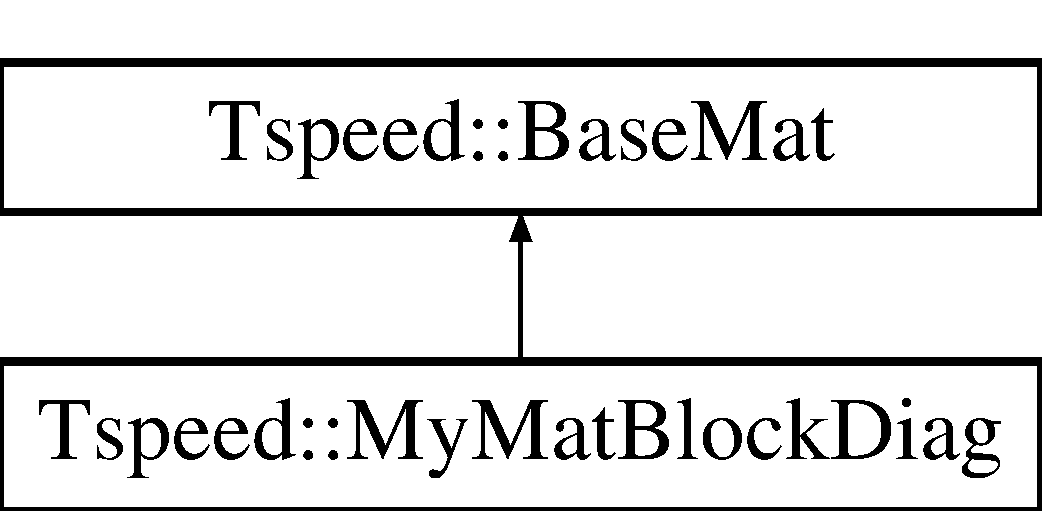
\includegraphics[height=2.000000cm]{classTspeed_1_1MyMatBlockDiag}
\end{center}
\end{figure}
\subsection*{Public Member Functions}
\begin{DoxyCompactItemize}
\item 
\hyperlink{classTspeed_1_1MyMatBlockDiag_a1edd89c439245f97a1cbfcf81b588211}{My\-Mat\-Block\-Diag} ()
\item 
\hyperlink{classTspeed_1_1MyMatBlockDiag_a2d740a6b014d37383f751b312ccdf66e}{My\-Mat\-Block\-Diag} (\hyperlink{namespaceTspeed_a7367a01365c4cc2c1a09305b3effc4e8}{Mesh\-\_\-ptr}, unsigned int nln)
\item 
\hyperlink{classTspeed_1_1MyMatBlockDiag_ae115b76e406285af1c3d41682ecc359c}{My\-Mat\-Block\-Diag} (\hyperlink{classTspeed_1_1MyMatBlockDiag}{My\-Mat\-Block\-Diag} \&\&)=default
\item 
\hyperlink{classTspeed_1_1MyMatBlockDiag_af6f41226563ccd37cc0113a50af2e0e7}{My\-Mat\-Block\-Diag} (\hyperlink{classTspeed_1_1MyMatBlockDiag}{My\-Mat\-Block\-Diag} const \&)=default
\item 
\hyperlink{classTspeed_1_1MyMatBlockDiag}{My\-Mat\-Block\-Diag} \& \hyperlink{classTspeed_1_1MyMatBlockDiag_a7e7efacca7a0a45f0df066155008ed36}{operator=} (\hyperlink{classTspeed_1_1MyMatBlockDiag}{My\-Mat\-Block\-Diag} \&\&)=default
\item 
\hyperlink{classTspeed_1_1MyMatBlockDiag}{My\-Mat\-Block\-Diag} \& \hyperlink{classTspeed_1_1MyMatBlockDiag_af98e9c0be1adb7bcdfc49f36f2e536d7}{operator=} (\hyperlink{classTspeed_1_1MyMatBlockDiag}{My\-Mat\-Block\-Diag} const \&)=default
\item 
virtual \hyperlink{classTspeed_1_1MyMatBlockDiag_a696ec354baf3873bf85a168a91e5afd7}{$\sim$\-My\-Mat\-Block\-Diag} () noexcept(true)=default
\end{DoxyCompactItemize}
\subsection*{Additional Inherited Members}


\subsection{Constructor \& Destructor Documentation}
\hypertarget{classTspeed_1_1MyMatBlockDiag_a1edd89c439245f97a1cbfcf81b588211}{\index{Tspeed\-::\-My\-Mat\-Block\-Diag@{Tspeed\-::\-My\-Mat\-Block\-Diag}!My\-Mat\-Block\-Diag@{My\-Mat\-Block\-Diag}}
\index{My\-Mat\-Block\-Diag@{My\-Mat\-Block\-Diag}!Tspeed::MyMatBlockDiag@{Tspeed\-::\-My\-Mat\-Block\-Diag}}
\subsubsection[{My\-Mat\-Block\-Diag}]{\setlength{\rightskip}{0pt plus 5cm}Tspeed\-::\-My\-Mat\-Block\-Diag\-::\-My\-Mat\-Block\-Diag (
\begin{DoxyParamCaption}
{}
\end{DoxyParamCaption}
)\hspace{0.3cm}{\ttfamily [inline]}}}\label{classTspeed_1_1MyMatBlockDiag_a1edd89c439245f97a1cbfcf81b588211}
\hypertarget{classTspeed_1_1MyMatBlockDiag_a2d740a6b014d37383f751b312ccdf66e}{\index{Tspeed\-::\-My\-Mat\-Block\-Diag@{Tspeed\-::\-My\-Mat\-Block\-Diag}!My\-Mat\-Block\-Diag@{My\-Mat\-Block\-Diag}}
\index{My\-Mat\-Block\-Diag@{My\-Mat\-Block\-Diag}!Tspeed::MyMatBlockDiag@{Tspeed\-::\-My\-Mat\-Block\-Diag}}
\subsubsection[{My\-Mat\-Block\-Diag}]{\setlength{\rightskip}{0pt plus 5cm}Tspeed\-::\-My\-Mat\-Block\-Diag\-::\-My\-Mat\-Block\-Diag (
\begin{DoxyParamCaption}
\item[{{\bf Mesh\-\_\-ptr}}]{Th, }
\item[{unsigned int}]{nln}
\end{DoxyParamCaption}
)}}\label{classTspeed_1_1MyMatBlockDiag_a2d740a6b014d37383f751b312ccdf66e}
\hypertarget{classTspeed_1_1MyMatBlockDiag_ae115b76e406285af1c3d41682ecc359c}{\index{Tspeed\-::\-My\-Mat\-Block\-Diag@{Tspeed\-::\-My\-Mat\-Block\-Diag}!My\-Mat\-Block\-Diag@{My\-Mat\-Block\-Diag}}
\index{My\-Mat\-Block\-Diag@{My\-Mat\-Block\-Diag}!Tspeed::MyMatBlockDiag@{Tspeed\-::\-My\-Mat\-Block\-Diag}}
\subsubsection[{My\-Mat\-Block\-Diag}]{\setlength{\rightskip}{0pt plus 5cm}Tspeed\-::\-My\-Mat\-Block\-Diag\-::\-My\-Mat\-Block\-Diag (
\begin{DoxyParamCaption}
\item[{{\bf My\-Mat\-Block\-Diag} \&\&}]{}
\end{DoxyParamCaption}
)\hspace{0.3cm}{\ttfamily [default]}}}\label{classTspeed_1_1MyMatBlockDiag_ae115b76e406285af1c3d41682ecc359c}
\hypertarget{classTspeed_1_1MyMatBlockDiag_af6f41226563ccd37cc0113a50af2e0e7}{\index{Tspeed\-::\-My\-Mat\-Block\-Diag@{Tspeed\-::\-My\-Mat\-Block\-Diag}!My\-Mat\-Block\-Diag@{My\-Mat\-Block\-Diag}}
\index{My\-Mat\-Block\-Diag@{My\-Mat\-Block\-Diag}!Tspeed::MyMatBlockDiag@{Tspeed\-::\-My\-Mat\-Block\-Diag}}
\subsubsection[{My\-Mat\-Block\-Diag}]{\setlength{\rightskip}{0pt plus 5cm}Tspeed\-::\-My\-Mat\-Block\-Diag\-::\-My\-Mat\-Block\-Diag (
\begin{DoxyParamCaption}
\item[{{\bf My\-Mat\-Block\-Diag} const \&}]{}
\end{DoxyParamCaption}
)\hspace{0.3cm}{\ttfamily [default]}}}\label{classTspeed_1_1MyMatBlockDiag_af6f41226563ccd37cc0113a50af2e0e7}
\hypertarget{classTspeed_1_1MyMatBlockDiag_a696ec354baf3873bf85a168a91e5afd7}{\index{Tspeed\-::\-My\-Mat\-Block\-Diag@{Tspeed\-::\-My\-Mat\-Block\-Diag}!$\sim$\-My\-Mat\-Block\-Diag@{$\sim$\-My\-Mat\-Block\-Diag}}
\index{$\sim$\-My\-Mat\-Block\-Diag@{$\sim$\-My\-Mat\-Block\-Diag}!Tspeed::MyMatBlockDiag@{Tspeed\-::\-My\-Mat\-Block\-Diag}}
\subsubsection[{$\sim$\-My\-Mat\-Block\-Diag}]{\setlength{\rightskip}{0pt plus 5cm}virtual Tspeed\-::\-My\-Mat\-Block\-Diag\-::$\sim$\-My\-Mat\-Block\-Diag (
\begin{DoxyParamCaption}
{}
\end{DoxyParamCaption}
)\hspace{0.3cm}{\ttfamily [virtual]}, {\ttfamily [default]}, {\ttfamily [noexcept]}}}\label{classTspeed_1_1MyMatBlockDiag_a696ec354baf3873bf85a168a91e5afd7}


\subsection{Member Function Documentation}
\hypertarget{classTspeed_1_1MyMatBlockDiag_a7e7efacca7a0a45f0df066155008ed36}{\index{Tspeed\-::\-My\-Mat\-Block\-Diag@{Tspeed\-::\-My\-Mat\-Block\-Diag}!operator=@{operator=}}
\index{operator=@{operator=}!Tspeed::MyMatBlockDiag@{Tspeed\-::\-My\-Mat\-Block\-Diag}}
\subsubsection[{operator=}]{\setlength{\rightskip}{0pt plus 5cm}{\bf My\-Mat\-Block\-Diag}\& Tspeed\-::\-My\-Mat\-Block\-Diag\-::operator= (
\begin{DoxyParamCaption}
\item[{{\bf My\-Mat\-Block\-Diag} \&\&}]{}
\end{DoxyParamCaption}
)\hspace{0.3cm}{\ttfamily [default]}}}\label{classTspeed_1_1MyMatBlockDiag_a7e7efacca7a0a45f0df066155008ed36}
\hypertarget{classTspeed_1_1MyMatBlockDiag_af98e9c0be1adb7bcdfc49f36f2e536d7}{\index{Tspeed\-::\-My\-Mat\-Block\-Diag@{Tspeed\-::\-My\-Mat\-Block\-Diag}!operator=@{operator=}}
\index{operator=@{operator=}!Tspeed::MyMatBlockDiag@{Tspeed\-::\-My\-Mat\-Block\-Diag}}
\subsubsection[{operator=}]{\setlength{\rightskip}{0pt plus 5cm}{\bf My\-Mat\-Block\-Diag}\& Tspeed\-::\-My\-Mat\-Block\-Diag\-::operator= (
\begin{DoxyParamCaption}
\item[{{\bf My\-Mat\-Block\-Diag} const \&}]{}
\end{DoxyParamCaption}
)\hspace{0.3cm}{\ttfamily [default]}}}\label{classTspeed_1_1MyMatBlockDiag_af98e9c0be1adb7bcdfc49f36f2e536d7}


The documentation for this class was generated from the following files\-:\begin{DoxyCompactItemize}
\item 
lib/include/\hyperlink{MyMat_8hpp}{My\-Mat.\-hpp}\item 
lib/src/\hyperlink{MyMat_8cpp}{My\-Mat.\-cpp}\end{DoxyCompactItemize}

\hypertarget{classTspeed_1_1MyMatMultiDim}{\section{Tspeed\-:\-:My\-Mat\-Multi\-Dim$<$ T $>$ Class Template Reference}
\label{classTspeed_1_1MyMatMultiDim}\index{Tspeed\-::\-My\-Mat\-Multi\-Dim$<$ T $>$@{Tspeed\-::\-My\-Mat\-Multi\-Dim$<$ T $>$}}
}


{\ttfamily \#include $<$My\-Mat.\-hpp$>$}

\subsection*{Public Member Functions}
\begin{DoxyCompactItemize}
\item 
\hyperlink{classTspeed_1_1MyMatMultiDim_a1d08f2d14a8074dbfc0fb0ccf85c5bd3}{My\-Mat\-Multi\-Dim} ()=default
\item 
virtual \hyperlink{classTspeed_1_1MyMatMultiDim_a1186b247ce40afb915e3fac80f99deb3}{$\sim$\-My\-Mat\-Multi\-Dim} ()=default
\item 
\hyperlink{classTspeed_1_1MyMatMultiDim_aae1c5f412040fbc3f344f612b4609f95}{My\-Mat\-Multi\-Dim} (\hyperlink{namespaceTspeed_a7367a01365c4cc2c1a09305b3effc4e8}{Mesh\-\_\-ptr}, unsigned int nln)
\item 
T \& \hyperlink{classTspeed_1_1MyMatMultiDim_a03782558106363767dd160f5170e6a66}{component} (int \hyperlink{vtk__vector__out_8m_a6f6ccfcf58b31cb6412107d9d5281426}{i}, int \hyperlink{vtk__mesh__out_8m_af1af736f0a1475ea44566768103395cb}{j})
\item 
T const \& \hyperlink{classTspeed_1_1MyMatMultiDim_a4d217bb29f278fb65a8f02df72bf7142}{component} (int \hyperlink{vtk__vector__out_8m_a6f6ccfcf58b31cb6412107d9d5281426}{i}, int \hyperlink{vtk__mesh__out_8m_af1af736f0a1475ea44566768103395cb}{j}) const 
\item 
void \hyperlink{classTspeed_1_1MyMatMultiDim_a9e0b39723d52237575763129f4056349}{symmetrize} ()
\item 
void \hyperlink{classTspeed_1_1MyMatMultiDim_aac722312a8618d4c00033c9f6a86f7f7}{vec\-Mult} (Eigen\-::\-Vector\-Xd const \&, Eigen\-::\-Vector\-Xd \&) const 
\item 
\hyperlink{classTspeed_1_1MyMatMultiDim_a34932323d5f4aff040b1e85f5a89d341}{My\-Mat\-Multi\-Dim} (\hyperlink{classTspeed_1_1MyMatMultiDim}{My\-Mat\-Multi\-Dim} \&\hyperlink{load__and__plot__lamb_8m_aa875ab3a8009406dcace7fa71a0f490d}{a})
\item 
\hyperlink{classTspeed_1_1MyMatMultiDim}{My\-Mat\-Multi\-Dim} \& \hyperlink{classTspeed_1_1MyMatMultiDim_aadd37f5678750bbda4b536ecc5a00851}{operator=} (\hyperlink{classTspeed_1_1MyMatMultiDim}{My\-Mat\-Multi\-Dim} \&\&)=default
\item 
Eigen\-::\-Vector\-Xd \hyperlink{classTspeed_1_1MyMatMultiDim_acc8cd12d144a32a4be0c2dcb015156df}{operator$\ast$} (Eigen\-::\-Vector\-Xd const \&v) const 
\end{DoxyCompactItemize}
\subsection*{Friends}
\begin{DoxyCompactItemize}
\item 
\hyperlink{classTspeed_1_1MyMatMultiDim}{My\-Mat\-Multi\-Dim}$<$ \hyperlink{classTspeed_1_1MyMat}{My\-Mat} $>$ \hyperlink{classTspeed_1_1MyMatMultiDim_a0f13d96f443b5d3fe2e0ce2f128f5c28}{operator+} (\hyperlink{classTspeed_1_1MyMatMultiDim}{My\-Mat\-Multi\-Dim}$<$ \hyperlink{classTspeed_1_1MyMat}{My\-Mat} $>$ const \&\hyperlink{load__and__plot__lamb_8m_aa875ab3a8009406dcace7fa71a0f490d}{a}, \hyperlink{classTspeed_1_1MyMatMultiDim}{My\-Mat\-Multi\-Dim}$<$ \hyperlink{classTspeed_1_1MyMat}{My\-Mat} $>$ const \&\hyperlink{load__and__plot__lamb_8m_a21c7e548e910bb7ce7dcea81de72c8f7}{b})
\item 
\hyperlink{classTspeed_1_1MyMatMultiDim}{My\-Mat\-Multi\-Dim}$<$ \hyperlink{classTspeed_1_1MyMat}{My\-Mat} $>$ \hyperlink{classTspeed_1_1MyMatMultiDim_afe46b501e059ef54cd6701bfae967263}{operator+} (\hyperlink{classTspeed_1_1MyMatMultiDim}{My\-Mat\-Multi\-Dim}$<$ \hyperlink{classTspeed_1_1MyMat}{My\-Mat} $>$ const \&\hyperlink{load__and__plot__lamb_8m_aa875ab3a8009406dcace7fa71a0f490d}{a}, \hyperlink{classTspeed_1_1MyMatMultiDim}{My\-Mat\-Multi\-Dim}$<$ \hyperlink{classTspeed_1_1MyMatBlockDiag}{My\-Mat\-Block\-Diag} $>$ const \&\hyperlink{load__and__plot__lamb_8m_a21c7e548e910bb7ce7dcea81de72c8f7}{b})
\item 
\hyperlink{classTspeed_1_1MyMatMultiDim}{My\-Mat\-Multi\-Dim}$<$ T $>$ \hyperlink{classTspeed_1_1MyMatMultiDim_a10bafacdfbbd9746fab2e746196f4229}{operator$\ast$} (double const \&\hyperlink{vtk__mesh__out_8m_ace4b66138f2e64832c951b1ba9ce24cc}{x}, \hyperlink{classTspeed_1_1MyMatMultiDim}{My\-Mat\-Multi\-Dim}$<$ T $>$ const \&A)
\end{DoxyCompactItemize}


\subsection{Constructor \& Destructor Documentation}
\hypertarget{classTspeed_1_1MyMatMultiDim_a1d08f2d14a8074dbfc0fb0ccf85c5bd3}{\index{Tspeed\-::\-My\-Mat\-Multi\-Dim@{Tspeed\-::\-My\-Mat\-Multi\-Dim}!My\-Mat\-Multi\-Dim@{My\-Mat\-Multi\-Dim}}
\index{My\-Mat\-Multi\-Dim@{My\-Mat\-Multi\-Dim}!Tspeed::MyMatMultiDim@{Tspeed\-::\-My\-Mat\-Multi\-Dim}}
\subsubsection[{My\-Mat\-Multi\-Dim}]{\setlength{\rightskip}{0pt plus 5cm}template$<$typename T$>$ {\bf Tspeed\-::\-My\-Mat\-Multi\-Dim}$<$ T $>$\-::{\bf My\-Mat\-Multi\-Dim} (
\begin{DoxyParamCaption}
{}
\end{DoxyParamCaption}
)\hspace{0.3cm}{\ttfamily [default]}}}\label{classTspeed_1_1MyMatMultiDim_a1d08f2d14a8074dbfc0fb0ccf85c5bd3}
\hypertarget{classTspeed_1_1MyMatMultiDim_a1186b247ce40afb915e3fac80f99deb3}{\index{Tspeed\-::\-My\-Mat\-Multi\-Dim@{Tspeed\-::\-My\-Mat\-Multi\-Dim}!$\sim$\-My\-Mat\-Multi\-Dim@{$\sim$\-My\-Mat\-Multi\-Dim}}
\index{$\sim$\-My\-Mat\-Multi\-Dim@{$\sim$\-My\-Mat\-Multi\-Dim}!Tspeed::MyMatMultiDim@{Tspeed\-::\-My\-Mat\-Multi\-Dim}}
\subsubsection[{$\sim$\-My\-Mat\-Multi\-Dim}]{\setlength{\rightskip}{0pt plus 5cm}template$<$typename T$>$ virtual {\bf Tspeed\-::\-My\-Mat\-Multi\-Dim}$<$ T $>$\-::$\sim${\bf My\-Mat\-Multi\-Dim} (
\begin{DoxyParamCaption}
{}
\end{DoxyParamCaption}
)\hspace{0.3cm}{\ttfamily [virtual]}, {\ttfamily [default]}}}\label{classTspeed_1_1MyMatMultiDim_a1186b247ce40afb915e3fac80f99deb3}
\hypertarget{classTspeed_1_1MyMatMultiDim_aae1c5f412040fbc3f344f612b4609f95}{\index{Tspeed\-::\-My\-Mat\-Multi\-Dim@{Tspeed\-::\-My\-Mat\-Multi\-Dim}!My\-Mat\-Multi\-Dim@{My\-Mat\-Multi\-Dim}}
\index{My\-Mat\-Multi\-Dim@{My\-Mat\-Multi\-Dim}!Tspeed::MyMatMultiDim@{Tspeed\-::\-My\-Mat\-Multi\-Dim}}
\subsubsection[{My\-Mat\-Multi\-Dim}]{\setlength{\rightskip}{0pt plus 5cm}template$<$typename T $>$ {\bf Tspeed\-::\-My\-Mat\-Multi\-Dim}$<$ T $>$\-::{\bf My\-Mat\-Multi\-Dim} (
\begin{DoxyParamCaption}
\item[{{\bf Mesh\-\_\-ptr}}]{m, }
\item[{unsigned int}]{nln}
\end{DoxyParamCaption}
)}}\label{classTspeed_1_1MyMatMultiDim_aae1c5f412040fbc3f344f612b4609f95}
\hypertarget{classTspeed_1_1MyMatMultiDim_a34932323d5f4aff040b1e85f5a89d341}{\index{Tspeed\-::\-My\-Mat\-Multi\-Dim@{Tspeed\-::\-My\-Mat\-Multi\-Dim}!My\-Mat\-Multi\-Dim@{My\-Mat\-Multi\-Dim}}
\index{My\-Mat\-Multi\-Dim@{My\-Mat\-Multi\-Dim}!Tspeed::MyMatMultiDim@{Tspeed\-::\-My\-Mat\-Multi\-Dim}}
\subsubsection[{My\-Mat\-Multi\-Dim}]{\setlength{\rightskip}{0pt plus 5cm}template$<$typename T$>$ {\bf Tspeed\-::\-My\-Mat\-Multi\-Dim}$<$ T $>$\-::{\bf My\-Mat\-Multi\-Dim} (
\begin{DoxyParamCaption}
\item[{{\bf My\-Mat\-Multi\-Dim}$<$ T $>$ \&}]{a}
\end{DoxyParamCaption}
)\hspace{0.3cm}{\ttfamily [inline]}}}\label{classTspeed_1_1MyMatMultiDim_a34932323d5f4aff040b1e85f5a89d341}


\subsection{Member Function Documentation}
\hypertarget{classTspeed_1_1MyMatMultiDim_a03782558106363767dd160f5170e6a66}{\index{Tspeed\-::\-My\-Mat\-Multi\-Dim@{Tspeed\-::\-My\-Mat\-Multi\-Dim}!component@{component}}
\index{component@{component}!Tspeed::MyMatMultiDim@{Tspeed\-::\-My\-Mat\-Multi\-Dim}}
\subsubsection[{component}]{\setlength{\rightskip}{0pt plus 5cm}template$<$typename T$>$ T\& {\bf Tspeed\-::\-My\-Mat\-Multi\-Dim}$<$ T $>$\-::component (
\begin{DoxyParamCaption}
\item[{int}]{i, }
\item[{int}]{j}
\end{DoxyParamCaption}
)\hspace{0.3cm}{\ttfamily [inline]}}}\label{classTspeed_1_1MyMatMultiDim_a03782558106363767dd160f5170e6a66}
\hypertarget{classTspeed_1_1MyMatMultiDim_a4d217bb29f278fb65a8f02df72bf7142}{\index{Tspeed\-::\-My\-Mat\-Multi\-Dim@{Tspeed\-::\-My\-Mat\-Multi\-Dim}!component@{component}}
\index{component@{component}!Tspeed::MyMatMultiDim@{Tspeed\-::\-My\-Mat\-Multi\-Dim}}
\subsubsection[{component}]{\setlength{\rightskip}{0pt plus 5cm}template$<$typename T$>$ T const\& {\bf Tspeed\-::\-My\-Mat\-Multi\-Dim}$<$ T $>$\-::component (
\begin{DoxyParamCaption}
\item[{int}]{i, }
\item[{int}]{j}
\end{DoxyParamCaption}
) const\hspace{0.3cm}{\ttfamily [inline]}}}\label{classTspeed_1_1MyMatMultiDim_a4d217bb29f278fb65a8f02df72bf7142}
\hypertarget{classTspeed_1_1MyMatMultiDim_acc8cd12d144a32a4be0c2dcb015156df}{\index{Tspeed\-::\-My\-Mat\-Multi\-Dim@{Tspeed\-::\-My\-Mat\-Multi\-Dim}!operator$\ast$@{operator$\ast$}}
\index{operator$\ast$@{operator$\ast$}!Tspeed::MyMatMultiDim@{Tspeed\-::\-My\-Mat\-Multi\-Dim}}
\subsubsection[{operator$\ast$}]{\setlength{\rightskip}{0pt plus 5cm}template$<$typename T $>$ Eigen\-::\-Vector\-Xd {\bf Tspeed\-::\-My\-Mat\-Multi\-Dim}$<$ T $>$\-::operator$\ast$ (
\begin{DoxyParamCaption}
\item[{Eigen\-::\-Vector\-Xd const \&}]{v}
\end{DoxyParamCaption}
) const}}\label{classTspeed_1_1MyMatMultiDim_acc8cd12d144a32a4be0c2dcb015156df}
\hypertarget{classTspeed_1_1MyMatMultiDim_aadd37f5678750bbda4b536ecc5a00851}{\index{Tspeed\-::\-My\-Mat\-Multi\-Dim@{Tspeed\-::\-My\-Mat\-Multi\-Dim}!operator=@{operator=}}
\index{operator=@{operator=}!Tspeed::MyMatMultiDim@{Tspeed\-::\-My\-Mat\-Multi\-Dim}}
\subsubsection[{operator=}]{\setlength{\rightskip}{0pt plus 5cm}template$<$typename T$>$ {\bf My\-Mat\-Multi\-Dim}\& {\bf Tspeed\-::\-My\-Mat\-Multi\-Dim}$<$ T $>$\-::operator= (
\begin{DoxyParamCaption}
\item[{{\bf My\-Mat\-Multi\-Dim}$<$ T $>$ \&\&}]{}
\end{DoxyParamCaption}
)\hspace{0.3cm}{\ttfamily [default]}}}\label{classTspeed_1_1MyMatMultiDim_aadd37f5678750bbda4b536ecc5a00851}
\hypertarget{classTspeed_1_1MyMatMultiDim_a9e0b39723d52237575763129f4056349}{\index{Tspeed\-::\-My\-Mat\-Multi\-Dim@{Tspeed\-::\-My\-Mat\-Multi\-Dim}!symmetrize@{symmetrize}}
\index{symmetrize@{symmetrize}!Tspeed::MyMatMultiDim@{Tspeed\-::\-My\-Mat\-Multi\-Dim}}
\subsubsection[{symmetrize}]{\setlength{\rightskip}{0pt plus 5cm}template$<$typename T $>$ void {\bf Tspeed\-::\-My\-Mat\-Multi\-Dim}$<$ T $>$\-::symmetrize (
\begin{DoxyParamCaption}
{}
\end{DoxyParamCaption}
)}}\label{classTspeed_1_1MyMatMultiDim_a9e0b39723d52237575763129f4056349}
\hypertarget{classTspeed_1_1MyMatMultiDim_aac722312a8618d4c00033c9f6a86f7f7}{\index{Tspeed\-::\-My\-Mat\-Multi\-Dim@{Tspeed\-::\-My\-Mat\-Multi\-Dim}!vec\-Mult@{vec\-Mult}}
\index{vec\-Mult@{vec\-Mult}!Tspeed::MyMatMultiDim@{Tspeed\-::\-My\-Mat\-Multi\-Dim}}
\subsubsection[{vec\-Mult}]{\setlength{\rightskip}{0pt plus 5cm}template$<$typename T $>$ void {\bf Tspeed\-::\-My\-Mat\-Multi\-Dim}$<$ T $>$\-::vec\-Mult (
\begin{DoxyParamCaption}
\item[{Eigen\-::\-Vector\-Xd const \&}]{x, }
\item[{Eigen\-::\-Vector\-Xd \&}]{out}
\end{DoxyParamCaption}
) const}}\label{classTspeed_1_1MyMatMultiDim_aac722312a8618d4c00033c9f6a86f7f7}


\subsection{Friends And Related Function Documentation}
\hypertarget{classTspeed_1_1MyMatMultiDim_a10bafacdfbbd9746fab2e746196f4229}{\index{Tspeed\-::\-My\-Mat\-Multi\-Dim@{Tspeed\-::\-My\-Mat\-Multi\-Dim}!operator$\ast$@{operator$\ast$}}
\index{operator$\ast$@{operator$\ast$}!Tspeed::MyMatMultiDim@{Tspeed\-::\-My\-Mat\-Multi\-Dim}}
\subsubsection[{operator$\ast$}]{\setlength{\rightskip}{0pt plus 5cm}template$<$typename T$>$ {\bf My\-Mat\-Multi\-Dim}$<$T$>$ operator$\ast$ (
\begin{DoxyParamCaption}
\item[{double const \&}]{x, }
\item[{{\bf My\-Mat\-Multi\-Dim}$<$ T $>$ const \&}]{A}
\end{DoxyParamCaption}
)\hspace{0.3cm}{\ttfamily [friend]}}}\label{classTspeed_1_1MyMatMultiDim_a10bafacdfbbd9746fab2e746196f4229}
\hypertarget{classTspeed_1_1MyMatMultiDim_a0f13d96f443b5d3fe2e0ce2f128f5c28}{\index{Tspeed\-::\-My\-Mat\-Multi\-Dim@{Tspeed\-::\-My\-Mat\-Multi\-Dim}!operator+@{operator+}}
\index{operator+@{operator+}!Tspeed::MyMatMultiDim@{Tspeed\-::\-My\-Mat\-Multi\-Dim}}
\subsubsection[{operator+}]{\setlength{\rightskip}{0pt plus 5cm}template$<$typename T$>$ {\bf My\-Mat\-Multi\-Dim}$<${\bf My\-Mat}$>$ operator+ (
\begin{DoxyParamCaption}
\item[{{\bf My\-Mat\-Multi\-Dim}$<$ {\bf My\-Mat} $>$ const \&}]{a, }
\item[{{\bf My\-Mat\-Multi\-Dim}$<$ {\bf My\-Mat} $>$ const \&}]{b}
\end{DoxyParamCaption}
)\hspace{0.3cm}{\ttfamily [friend]}}}\label{classTspeed_1_1MyMatMultiDim_a0f13d96f443b5d3fe2e0ce2f128f5c28}
\hypertarget{classTspeed_1_1MyMatMultiDim_afe46b501e059ef54cd6701bfae967263}{\index{Tspeed\-::\-My\-Mat\-Multi\-Dim@{Tspeed\-::\-My\-Mat\-Multi\-Dim}!operator+@{operator+}}
\index{operator+@{operator+}!Tspeed::MyMatMultiDim@{Tspeed\-::\-My\-Mat\-Multi\-Dim}}
\subsubsection[{operator+}]{\setlength{\rightskip}{0pt plus 5cm}template$<$typename T$>$ {\bf My\-Mat\-Multi\-Dim}$<${\bf My\-Mat}$>$ operator+ (
\begin{DoxyParamCaption}
\item[{{\bf My\-Mat\-Multi\-Dim}$<$ {\bf My\-Mat} $>$ const \&}]{a, }
\item[{{\bf My\-Mat\-Multi\-Dim}$<$ {\bf My\-Mat\-Block\-Diag} $>$ const \&}]{b}
\end{DoxyParamCaption}
)\hspace{0.3cm}{\ttfamily [friend]}}}\label{classTspeed_1_1MyMatMultiDim_afe46b501e059ef54cd6701bfae967263}


The documentation for this class was generated from the following file\-:\begin{DoxyCompactItemize}
\item 
lib/include/\hyperlink{MyMat_8hpp}{My\-Mat.\-hpp}\end{DoxyCompactItemize}

\hypertarget{classTspeed_1_1MyMatMultiDimBlockDiag}{\section{Tspeed\-:\-:My\-Mat\-Multi\-Dim\-Block\-Diag$<$ T $>$ Class Template Reference}
\label{classTspeed_1_1MyMatMultiDimBlockDiag}\index{Tspeed\-::\-My\-Mat\-Multi\-Dim\-Block\-Diag$<$ T $>$@{Tspeed\-::\-My\-Mat\-Multi\-Dim\-Block\-Diag$<$ T $>$}}
}


{\ttfamily \#include $<$My\-Mat.\-hpp$>$}

\subsection*{Public Member Functions}
\begin{DoxyCompactItemize}
\item 
\hyperlink{classTspeed_1_1MyMatMultiDimBlockDiag_afab5a0f9292e20682a092df2e23e4085}{My\-Mat\-Multi\-Dim\-Block\-Diag} ()=default
\item 
virtual \hyperlink{classTspeed_1_1MyMatMultiDimBlockDiag_a3571b43f213adf9d0a267cb0f51ffa17}{$\sim$\-My\-Mat\-Multi\-Dim\-Block\-Diag} ()=default
\item 
\hyperlink{classTspeed_1_1MyMatMultiDimBlockDiag_aced3b96e49bd12dfeb95f763fbd0757f}{My\-Mat\-Multi\-Dim\-Block\-Diag} (\hyperlink{namespaceTspeed_a7367a01365c4cc2c1a09305b3effc4e8}{Mesh\-\_\-ptr}, unsigned int nln)
\item 
T \& \hyperlink{classTspeed_1_1MyMatMultiDimBlockDiag_aa430ef9d18b0a68c4bff63047daf0be9}{component} (int \hyperlink{vtk__vector__out_8m_a6f6ccfcf58b31cb6412107d9d5281426}{i})
\item 
T const \& \hyperlink{classTspeed_1_1MyMatMultiDimBlockDiag_a5f813a4f7c0a080cb5e1808941ef7348}{component} (int \hyperlink{vtk__vector__out_8m_a6f6ccfcf58b31cb6412107d9d5281426}{i}) const 
\item 
void \hyperlink{classTspeed_1_1MyMatMultiDimBlockDiag_a4d495f30e8088fd75502fa035e719c14}{vec\-Mult} (Eigen\-::\-Vector\-Xd const \&, Eigen\-::\-Vector\-Xd \&) const 
\item 
\hyperlink{classTspeed_1_1MyMatMultiDimBlockDiag_a64aee8deb9a8477c247778c033dd54c0}{My\-Mat\-Multi\-Dim\-Block\-Diag} (\hyperlink{classTspeed_1_1MyMatMultiDimBlockDiag}{My\-Mat\-Multi\-Dim\-Block\-Diag} \&\&)=default
\item 
\hyperlink{classTspeed_1_1MyMatMultiDimBlockDiag}{My\-Mat\-Multi\-Dim\-Block\-Diag} \& \hyperlink{classTspeed_1_1MyMatMultiDimBlockDiag_a2cecd6795a391ecbf1853f8af8926277}{operator=} (\hyperlink{classTspeed_1_1MyMatMultiDimBlockDiag}{My\-Mat\-Multi\-Dim\-Block\-Diag} \&\&)=default
\item 
unsigned int \hyperlink{classTspeed_1_1MyMatMultiDimBlockDiag_a5016da7b2a0ff6099353ddd91f960dd7}{nr} () const 
\item 
Eigen\-::\-Vector\-Xd \hyperlink{classTspeed_1_1MyMatMultiDimBlockDiag_ae688f7b76e7da9686a74bed5d0f059c7}{operator$\ast$} (Eigen\-::\-Vector\-Xd const \&v) const 
\end{DoxyCompactItemize}
\subsection*{Friends}
\begin{DoxyCompactItemize}
\item 
\hyperlink{classTspeed_1_1MyMatMultiDimBlockDiag}{My\-Mat\-Multi\-Dim\-Block\-Diag} const \& \hyperlink{classTspeed_1_1MyMatMultiDimBlockDiag_a2be04a4f228649a2efc0af5ac011852e}{operator$\ast$} (double const \&\hyperlink{vtk__mesh__out_8m_ace4b66138f2e64832c951b1ba9ce24cc}{x}, \hyperlink{classTspeed_1_1MyMatMultiDimBlockDiag}{My\-Mat\-Multi\-Dim\-Block\-Diag} const \&A)
\end{DoxyCompactItemize}


\subsection{Constructor \& Destructor Documentation}
\hypertarget{classTspeed_1_1MyMatMultiDimBlockDiag_afab5a0f9292e20682a092df2e23e4085}{\index{Tspeed\-::\-My\-Mat\-Multi\-Dim\-Block\-Diag@{Tspeed\-::\-My\-Mat\-Multi\-Dim\-Block\-Diag}!My\-Mat\-Multi\-Dim\-Block\-Diag@{My\-Mat\-Multi\-Dim\-Block\-Diag}}
\index{My\-Mat\-Multi\-Dim\-Block\-Diag@{My\-Mat\-Multi\-Dim\-Block\-Diag}!Tspeed::MyMatMultiDimBlockDiag@{Tspeed\-::\-My\-Mat\-Multi\-Dim\-Block\-Diag}}
\subsubsection[{My\-Mat\-Multi\-Dim\-Block\-Diag}]{\setlength{\rightskip}{0pt plus 5cm}template$<$typename T$>$ {\bf Tspeed\-::\-My\-Mat\-Multi\-Dim\-Block\-Diag}$<$ T $>$\-::{\bf My\-Mat\-Multi\-Dim\-Block\-Diag} (
\begin{DoxyParamCaption}
{}
\end{DoxyParamCaption}
)\hspace{0.3cm}{\ttfamily [default]}}}\label{classTspeed_1_1MyMatMultiDimBlockDiag_afab5a0f9292e20682a092df2e23e4085}
\hypertarget{classTspeed_1_1MyMatMultiDimBlockDiag_a3571b43f213adf9d0a267cb0f51ffa17}{\index{Tspeed\-::\-My\-Mat\-Multi\-Dim\-Block\-Diag@{Tspeed\-::\-My\-Mat\-Multi\-Dim\-Block\-Diag}!$\sim$\-My\-Mat\-Multi\-Dim\-Block\-Diag@{$\sim$\-My\-Mat\-Multi\-Dim\-Block\-Diag}}
\index{$\sim$\-My\-Mat\-Multi\-Dim\-Block\-Diag@{$\sim$\-My\-Mat\-Multi\-Dim\-Block\-Diag}!Tspeed::MyMatMultiDimBlockDiag@{Tspeed\-::\-My\-Mat\-Multi\-Dim\-Block\-Diag}}
\subsubsection[{$\sim$\-My\-Mat\-Multi\-Dim\-Block\-Diag}]{\setlength{\rightskip}{0pt plus 5cm}template$<$typename T$>$ virtual {\bf Tspeed\-::\-My\-Mat\-Multi\-Dim\-Block\-Diag}$<$ T $>$\-::$\sim${\bf My\-Mat\-Multi\-Dim\-Block\-Diag} (
\begin{DoxyParamCaption}
{}
\end{DoxyParamCaption}
)\hspace{0.3cm}{\ttfamily [virtual]}, {\ttfamily [default]}}}\label{classTspeed_1_1MyMatMultiDimBlockDiag_a3571b43f213adf9d0a267cb0f51ffa17}
\hypertarget{classTspeed_1_1MyMatMultiDimBlockDiag_aced3b96e49bd12dfeb95f763fbd0757f}{\index{Tspeed\-::\-My\-Mat\-Multi\-Dim\-Block\-Diag@{Tspeed\-::\-My\-Mat\-Multi\-Dim\-Block\-Diag}!My\-Mat\-Multi\-Dim\-Block\-Diag@{My\-Mat\-Multi\-Dim\-Block\-Diag}}
\index{My\-Mat\-Multi\-Dim\-Block\-Diag@{My\-Mat\-Multi\-Dim\-Block\-Diag}!Tspeed::MyMatMultiDimBlockDiag@{Tspeed\-::\-My\-Mat\-Multi\-Dim\-Block\-Diag}}
\subsubsection[{My\-Mat\-Multi\-Dim\-Block\-Diag}]{\setlength{\rightskip}{0pt plus 5cm}template$<$typename T $>$ {\bf Tspeed\-::\-My\-Mat\-Multi\-Dim\-Block\-Diag}$<$ T $>$\-::{\bf My\-Mat\-Multi\-Dim\-Block\-Diag} (
\begin{DoxyParamCaption}
\item[{{\bf Mesh\-\_\-ptr}}]{m, }
\item[{unsigned int}]{nln}
\end{DoxyParamCaption}
)}}\label{classTspeed_1_1MyMatMultiDimBlockDiag_aced3b96e49bd12dfeb95f763fbd0757f}
\hypertarget{classTspeed_1_1MyMatMultiDimBlockDiag_a64aee8deb9a8477c247778c033dd54c0}{\index{Tspeed\-::\-My\-Mat\-Multi\-Dim\-Block\-Diag@{Tspeed\-::\-My\-Mat\-Multi\-Dim\-Block\-Diag}!My\-Mat\-Multi\-Dim\-Block\-Diag@{My\-Mat\-Multi\-Dim\-Block\-Diag}}
\index{My\-Mat\-Multi\-Dim\-Block\-Diag@{My\-Mat\-Multi\-Dim\-Block\-Diag}!Tspeed::MyMatMultiDimBlockDiag@{Tspeed\-::\-My\-Mat\-Multi\-Dim\-Block\-Diag}}
\subsubsection[{My\-Mat\-Multi\-Dim\-Block\-Diag}]{\setlength{\rightskip}{0pt plus 5cm}template$<$typename T$>$ {\bf Tspeed\-::\-My\-Mat\-Multi\-Dim\-Block\-Diag}$<$ T $>$\-::{\bf My\-Mat\-Multi\-Dim\-Block\-Diag} (
\begin{DoxyParamCaption}
\item[{{\bf My\-Mat\-Multi\-Dim\-Block\-Diag}$<$ T $>$ \&\&}]{}
\end{DoxyParamCaption}
)\hspace{0.3cm}{\ttfamily [default]}}}\label{classTspeed_1_1MyMatMultiDimBlockDiag_a64aee8deb9a8477c247778c033dd54c0}


\subsection{Member Function Documentation}
\hypertarget{classTspeed_1_1MyMatMultiDimBlockDiag_aa430ef9d18b0a68c4bff63047daf0be9}{\index{Tspeed\-::\-My\-Mat\-Multi\-Dim\-Block\-Diag@{Tspeed\-::\-My\-Mat\-Multi\-Dim\-Block\-Diag}!component@{component}}
\index{component@{component}!Tspeed::MyMatMultiDimBlockDiag@{Tspeed\-::\-My\-Mat\-Multi\-Dim\-Block\-Diag}}
\subsubsection[{component}]{\setlength{\rightskip}{0pt plus 5cm}template$<$typename T$>$ T\& {\bf Tspeed\-::\-My\-Mat\-Multi\-Dim\-Block\-Diag}$<$ T $>$\-::component (
\begin{DoxyParamCaption}
\item[{int}]{i}
\end{DoxyParamCaption}
)\hspace{0.3cm}{\ttfamily [inline]}}}\label{classTspeed_1_1MyMatMultiDimBlockDiag_aa430ef9d18b0a68c4bff63047daf0be9}
\hypertarget{classTspeed_1_1MyMatMultiDimBlockDiag_a5f813a4f7c0a080cb5e1808941ef7348}{\index{Tspeed\-::\-My\-Mat\-Multi\-Dim\-Block\-Diag@{Tspeed\-::\-My\-Mat\-Multi\-Dim\-Block\-Diag}!component@{component}}
\index{component@{component}!Tspeed::MyMatMultiDimBlockDiag@{Tspeed\-::\-My\-Mat\-Multi\-Dim\-Block\-Diag}}
\subsubsection[{component}]{\setlength{\rightskip}{0pt plus 5cm}template$<$typename T$>$ T const\& {\bf Tspeed\-::\-My\-Mat\-Multi\-Dim\-Block\-Diag}$<$ T $>$\-::component (
\begin{DoxyParamCaption}
\item[{int}]{i}
\end{DoxyParamCaption}
) const\hspace{0.3cm}{\ttfamily [inline]}}}\label{classTspeed_1_1MyMatMultiDimBlockDiag_a5f813a4f7c0a080cb5e1808941ef7348}
\hypertarget{classTspeed_1_1MyMatMultiDimBlockDiag_a5016da7b2a0ff6099353ddd91f960dd7}{\index{Tspeed\-::\-My\-Mat\-Multi\-Dim\-Block\-Diag@{Tspeed\-::\-My\-Mat\-Multi\-Dim\-Block\-Diag}!nr@{nr}}
\index{nr@{nr}!Tspeed::MyMatMultiDimBlockDiag@{Tspeed\-::\-My\-Mat\-Multi\-Dim\-Block\-Diag}}
\subsubsection[{nr}]{\setlength{\rightskip}{0pt plus 5cm}template$<$typename T$>$ unsigned int {\bf Tspeed\-::\-My\-Mat\-Multi\-Dim\-Block\-Diag}$<$ T $>$\-::nr (
\begin{DoxyParamCaption}
{}
\end{DoxyParamCaption}
) const\hspace{0.3cm}{\ttfamily [inline]}}}\label{classTspeed_1_1MyMatMultiDimBlockDiag_a5016da7b2a0ff6099353ddd91f960dd7}
\hypertarget{classTspeed_1_1MyMatMultiDimBlockDiag_ae688f7b76e7da9686a74bed5d0f059c7}{\index{Tspeed\-::\-My\-Mat\-Multi\-Dim\-Block\-Diag@{Tspeed\-::\-My\-Mat\-Multi\-Dim\-Block\-Diag}!operator$\ast$@{operator$\ast$}}
\index{operator$\ast$@{operator$\ast$}!Tspeed::MyMatMultiDimBlockDiag@{Tspeed\-::\-My\-Mat\-Multi\-Dim\-Block\-Diag}}
\subsubsection[{operator$\ast$}]{\setlength{\rightskip}{0pt plus 5cm}template$<$typename T $>$ Eigen\-::\-Vector\-Xd {\bf Tspeed\-::\-My\-Mat\-Multi\-Dim\-Block\-Diag}$<$ T $>$\-::operator$\ast$ (
\begin{DoxyParamCaption}
\item[{Eigen\-::\-Vector\-Xd const \&}]{v}
\end{DoxyParamCaption}
) const}}\label{classTspeed_1_1MyMatMultiDimBlockDiag_ae688f7b76e7da9686a74bed5d0f059c7}
\hypertarget{classTspeed_1_1MyMatMultiDimBlockDiag_a2cecd6795a391ecbf1853f8af8926277}{\index{Tspeed\-::\-My\-Mat\-Multi\-Dim\-Block\-Diag@{Tspeed\-::\-My\-Mat\-Multi\-Dim\-Block\-Diag}!operator=@{operator=}}
\index{operator=@{operator=}!Tspeed::MyMatMultiDimBlockDiag@{Tspeed\-::\-My\-Mat\-Multi\-Dim\-Block\-Diag}}
\subsubsection[{operator=}]{\setlength{\rightskip}{0pt plus 5cm}template$<$typename T$>$ {\bf My\-Mat\-Multi\-Dim\-Block\-Diag}\& {\bf Tspeed\-::\-My\-Mat\-Multi\-Dim\-Block\-Diag}$<$ T $>$\-::operator= (
\begin{DoxyParamCaption}
\item[{{\bf My\-Mat\-Multi\-Dim\-Block\-Diag}$<$ T $>$ \&\&}]{}
\end{DoxyParamCaption}
)\hspace{0.3cm}{\ttfamily [default]}}}\label{classTspeed_1_1MyMatMultiDimBlockDiag_a2cecd6795a391ecbf1853f8af8926277}
\hypertarget{classTspeed_1_1MyMatMultiDimBlockDiag_a4d495f30e8088fd75502fa035e719c14}{\index{Tspeed\-::\-My\-Mat\-Multi\-Dim\-Block\-Diag@{Tspeed\-::\-My\-Mat\-Multi\-Dim\-Block\-Diag}!vec\-Mult@{vec\-Mult}}
\index{vec\-Mult@{vec\-Mult}!Tspeed::MyMatMultiDimBlockDiag@{Tspeed\-::\-My\-Mat\-Multi\-Dim\-Block\-Diag}}
\subsubsection[{vec\-Mult}]{\setlength{\rightskip}{0pt plus 5cm}template$<$typename T $>$ void {\bf Tspeed\-::\-My\-Mat\-Multi\-Dim\-Block\-Diag}$<$ T $>$\-::vec\-Mult (
\begin{DoxyParamCaption}
\item[{Eigen\-::\-Vector\-Xd const \&}]{x, }
\item[{Eigen\-::\-Vector\-Xd \&}]{out}
\end{DoxyParamCaption}
) const}}\label{classTspeed_1_1MyMatMultiDimBlockDiag_a4d495f30e8088fd75502fa035e719c14}


\subsection{Friends And Related Function Documentation}
\hypertarget{classTspeed_1_1MyMatMultiDimBlockDiag_a2be04a4f228649a2efc0af5ac011852e}{\index{Tspeed\-::\-My\-Mat\-Multi\-Dim\-Block\-Diag@{Tspeed\-::\-My\-Mat\-Multi\-Dim\-Block\-Diag}!operator$\ast$@{operator$\ast$}}
\index{operator$\ast$@{operator$\ast$}!Tspeed::MyMatMultiDimBlockDiag@{Tspeed\-::\-My\-Mat\-Multi\-Dim\-Block\-Diag}}
\subsubsection[{operator$\ast$}]{\setlength{\rightskip}{0pt plus 5cm}template$<$typename T$>$ {\bf My\-Mat\-Multi\-Dim\-Block\-Diag} const\& operator$\ast$ (
\begin{DoxyParamCaption}
\item[{double const \&}]{x, }
\item[{{\bf My\-Mat\-Multi\-Dim\-Block\-Diag}$<$ T $>$ const \&}]{A}
\end{DoxyParamCaption}
)\hspace{0.3cm}{\ttfamily [friend]}}}\label{classTspeed_1_1MyMatMultiDimBlockDiag_a2be04a4f228649a2efc0af5ac011852e}


The documentation for this class was generated from the following file\-:\begin{DoxyCompactItemize}
\item 
lib/include/\hyperlink{MyMat_8hpp}{My\-Mat.\-hpp}\end{DoxyCompactItemize}

\hypertarget{classTspeed_1_1Parameters}{\section{Tspeed\-:\-:Parameters Class Reference}
\label{classTspeed_1_1Parameters}\index{Tspeed\-::\-Parameters@{Tspeed\-::\-Parameters}}
}


Class for the parameters $\lambda, \rho, \mu$ of the elastodynamics equations.  




{\ttfamily \#include $<$F\-E\-Space.\-hpp$>$}

\subsection*{Public Member Functions}
\begin{DoxyCompactItemize}
\item 
virtual \hyperlink{classTspeed_1_1Parameters_ad15fb30d29239fb9d5f6ae2d95448e0b}{$\sim$\-Parameters} ()
\item 
\hyperlink{classTspeed_1_1Parameters_a9532e35c18436a3ffa9df32e5124b8cf}{Parameters} (\hyperlink{namespaceTspeed_a7367a01365c4cc2c1a09305b3effc4e8}{Mesh\-\_\-ptr} m)
\item 
void \hyperlink{classTspeed_1_1Parameters_a3f92e66ca503e376f51cdceebdc1afaa}{setp} (std\-::string const \&p, int const lab, double const \hyperlink{classTspeed_1_1Parameters_aec8ee931eddac3812e09db45a412685d}{lambda})
\begin{DoxyCompactList}\small\item\em Set a parameter. \end{DoxyCompactList}\item 
double const \& \hyperlink{classTspeed_1_1Parameters_aec8ee931eddac3812e09db45a412685d}{lambda} (int i) const 
\begin{DoxyCompactList}\small\item\em Get lambda on element i. \end{DoxyCompactList}\item 
double const \& \hyperlink{classTspeed_1_1Parameters_a4edca911ff34296039e07b9665ebcfa1}{mu} (int i) const 
\begin{DoxyCompactList}\small\item\em Get mu on element i. \end{DoxyCompactList}\item 
double const \& \hyperlink{classTspeed_1_1Parameters_ad111ae3220d2ff1c68130d9dee83665e}{rho} (int i) const 
\begin{DoxyCompactList}\small\item\em Get rho on element i. \end{DoxyCompactList}\item 
double \hyperlink{classTspeed_1_1Parameters_a9e3e70a0fd2c8aae9af142069c744cbb}{avg\-\_\-p} (std\-::string const \&p, int i, int j) const 
\begin{DoxyCompactList}\small\item\em Get the value of the harmonic average of a parameter between two elements. \end{DoxyCompactList}\end{DoxyCompactItemize}


\subsection{Detailed Description}
Class for the parameters $\lambda, \rho, \mu$ of the elastodynamics equations. 

\subsection{Constructor \& Destructor Documentation}
\hypertarget{classTspeed_1_1Parameters_ad15fb30d29239fb9d5f6ae2d95448e0b}{\index{Tspeed\-::\-Parameters@{Tspeed\-::\-Parameters}!$\sim$\-Parameters@{$\sim$\-Parameters}}
\index{$\sim$\-Parameters@{$\sim$\-Parameters}!Tspeed::Parameters@{Tspeed\-::\-Parameters}}
\subsubsection[{$\sim$\-Parameters}]{\setlength{\rightskip}{0pt plus 5cm}virtual Tspeed\-::\-Parameters\-::$\sim$\-Parameters (
\begin{DoxyParamCaption}
{}
\end{DoxyParamCaption}
)\hspace{0.3cm}{\ttfamily [inline]}, {\ttfamily [virtual]}}}\label{classTspeed_1_1Parameters_ad15fb30d29239fb9d5f6ae2d95448e0b}
\hypertarget{classTspeed_1_1Parameters_a9532e35c18436a3ffa9df32e5124b8cf}{\index{Tspeed\-::\-Parameters@{Tspeed\-::\-Parameters}!Parameters@{Parameters}}
\index{Parameters@{Parameters}!Tspeed::Parameters@{Tspeed\-::\-Parameters}}
\subsubsection[{Parameters}]{\setlength{\rightskip}{0pt plus 5cm}Tspeed\-::\-Parameters\-::\-Parameters (
\begin{DoxyParamCaption}
\item[{{\bf Mesh\-\_\-ptr}}]{m}
\end{DoxyParamCaption}
)\hspace{0.3cm}{\ttfamily [inline]}}}\label{classTspeed_1_1Parameters_a9532e35c18436a3ffa9df32e5124b8cf}


\subsection{Member Function Documentation}
\hypertarget{classTspeed_1_1Parameters_a9e3e70a0fd2c8aae9af142069c744cbb}{\index{Tspeed\-::\-Parameters@{Tspeed\-::\-Parameters}!avg\-\_\-p@{avg\-\_\-p}}
\index{avg\-\_\-p@{avg\-\_\-p}!Tspeed::Parameters@{Tspeed\-::\-Parameters}}
\subsubsection[{avg\-\_\-p}]{\setlength{\rightskip}{0pt plus 5cm}double Tspeed\-::\-Parameters\-::avg\-\_\-p (
\begin{DoxyParamCaption}
\item[{std\-::string const \&}]{p, }
\item[{int}]{i, }
\item[{int}]{j}
\end{DoxyParamCaption}
) const}}\label{classTspeed_1_1Parameters_a9e3e70a0fd2c8aae9af142069c744cbb}


Get the value of the harmonic average of a parameter between two elements. 


\begin{DoxyParams}{Parameters}
{\em p} & string with the name of the parameter (\char`\"{}lambda\char`\"{}, \char`\"{}mu\char`\"{}, \char`\"{}rho\char`\"{}) \\
\hline
{\em i} & index of one element \\
\hline
{\em j} & index of the seocnd element\\
\hline
\end{DoxyParams}
\begin{DoxyReturn}{Returns}
harmonic average 
\end{DoxyReturn}
\hypertarget{classTspeed_1_1Parameters_aec8ee931eddac3812e09db45a412685d}{\index{Tspeed\-::\-Parameters@{Tspeed\-::\-Parameters}!lambda@{lambda}}
\index{lambda@{lambda}!Tspeed::Parameters@{Tspeed\-::\-Parameters}}
\subsubsection[{lambda}]{\setlength{\rightskip}{0pt plus 5cm}double const\& Tspeed\-::\-Parameters\-::lambda (
\begin{DoxyParamCaption}
\item[{int}]{i}
\end{DoxyParamCaption}
) const\hspace{0.3cm}{\ttfamily [inline]}}}\label{classTspeed_1_1Parameters_aec8ee931eddac3812e09db45a412685d}


Get lambda on element i. 


\begin{DoxyParams}{Parameters}
{\em i} & the index of the element \\
\hline
\end{DoxyParams}
\hypertarget{classTspeed_1_1Parameters_a4edca911ff34296039e07b9665ebcfa1}{\index{Tspeed\-::\-Parameters@{Tspeed\-::\-Parameters}!mu@{mu}}
\index{mu@{mu}!Tspeed::Parameters@{Tspeed\-::\-Parameters}}
\subsubsection[{mu}]{\setlength{\rightskip}{0pt plus 5cm}double const\& Tspeed\-::\-Parameters\-::mu (
\begin{DoxyParamCaption}
\item[{int}]{i}
\end{DoxyParamCaption}
) const\hspace{0.3cm}{\ttfamily [inline]}}}\label{classTspeed_1_1Parameters_a4edca911ff34296039e07b9665ebcfa1}


Get mu on element i. 


\begin{DoxyParams}{Parameters}
{\em i} & the index of the element \\
\hline
\end{DoxyParams}
\hypertarget{classTspeed_1_1Parameters_ad111ae3220d2ff1c68130d9dee83665e}{\index{Tspeed\-::\-Parameters@{Tspeed\-::\-Parameters}!rho@{rho}}
\index{rho@{rho}!Tspeed::Parameters@{Tspeed\-::\-Parameters}}
\subsubsection[{rho}]{\setlength{\rightskip}{0pt plus 5cm}double const\& Tspeed\-::\-Parameters\-::rho (
\begin{DoxyParamCaption}
\item[{int}]{i}
\end{DoxyParamCaption}
) const\hspace{0.3cm}{\ttfamily [inline]}}}\label{classTspeed_1_1Parameters_ad111ae3220d2ff1c68130d9dee83665e}


Get rho on element i. 


\begin{DoxyParams}{Parameters}
{\em i} & the index of the element \\
\hline
\end{DoxyParams}
\hypertarget{classTspeed_1_1Parameters_a3f92e66ca503e376f51cdceebdc1afaa}{\index{Tspeed\-::\-Parameters@{Tspeed\-::\-Parameters}!setp@{setp}}
\index{setp@{setp}!Tspeed::Parameters@{Tspeed\-::\-Parameters}}
\subsubsection[{setp}]{\setlength{\rightskip}{0pt plus 5cm}void Tspeed\-::\-Parameters\-::setp (
\begin{DoxyParamCaption}
\item[{std\-::string const \&}]{p, }
\item[{int const}]{lab, }
\item[{double const}]{lambda}
\end{DoxyParamCaption}
)}}\label{classTspeed_1_1Parameters_a3f92e66ca503e376f51cdceebdc1afaa}


Set a parameter. 


\begin{DoxyParams}{Parameters}
{\em p} & string with the name of the parameter (\char`\"{}lambda\char`\"{}, \char`\"{}mu\char`\"{}, \char`\"{}rho\char`\"{}) \\
\hline
{\em lab} & attribute of the mesh partition on which the parameter is set \\
\hline
{\em lambda} & value of the parameter \\
\hline
\end{DoxyParams}


The documentation for this class was generated from the following files\-:\begin{DoxyCompactItemize}
\item 
lib/include/\hyperlink{FESpace_8hpp}{F\-E\-Space.\-hpp}\item 
lib/src/\hyperlink{Parameters_8cpp}{Parameters.\-cpp}\end{DoxyCompactItemize}

\hypertarget{classTspeed_1_1Geo_1_1Point}{\section{Tspeed\-:\-:Geo\-:\-:Point Class Reference}
\label{classTspeed_1_1Geo_1_1Point}\index{Tspeed\-::\-Geo\-::\-Point@{Tspeed\-::\-Geo\-::\-Point}}
}


{\ttfamily \#include $<$Geometry.\-hpp$>$}

Inheritance diagram for Tspeed\-:\-:Geo\-:\-:Point\-:\begin{figure}[H]
\begin{center}
\leavevmode
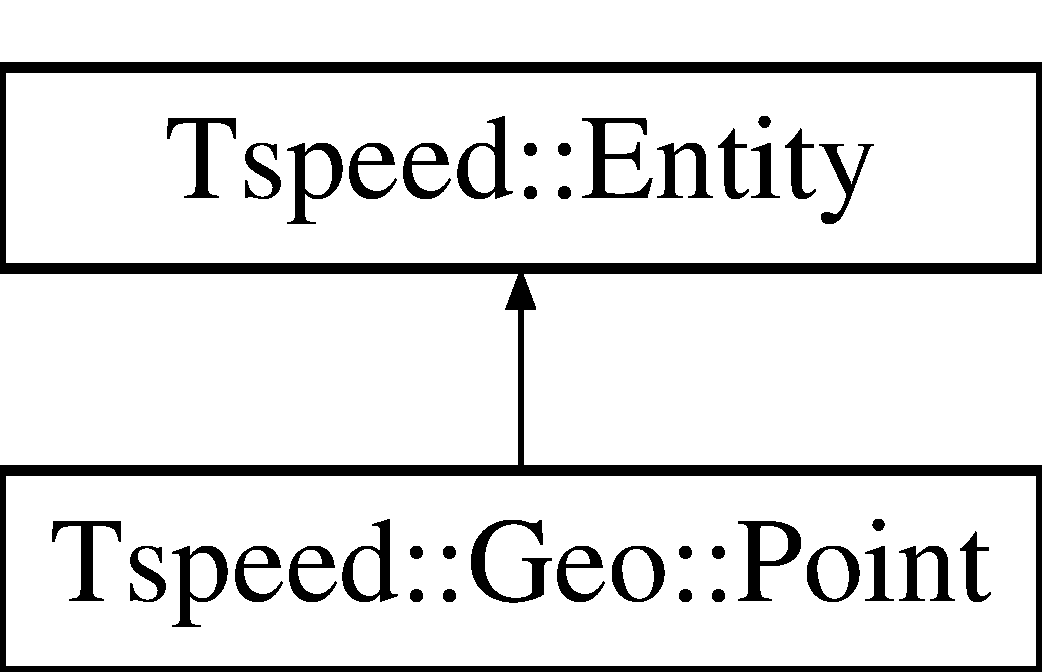
\includegraphics[height=2.000000cm]{classTspeed_1_1Geo_1_1Point}
\end{center}
\end{figure}
\subsection*{Public Member Functions}
\begin{DoxyCompactItemize}
\item 
\hyperlink{classTspeed_1_1Geo_1_1Point_a1d341df68317135dd9f7f39a172fd2d6}{Point} (const double \&\hyperlink{classTspeed_1_1Geo_1_1Point_a658f2ac4d36ea76832a36d8a4b0bcf96}{x}=0, const double \&\hyperlink{classTspeed_1_1Geo_1_1Point_a1424ccbaba0dbed5605d99f4718774ed}{y}=0)
\item 
\hyperlink{classTspeed_1_1Geo_1_1Point_a2d4ba9608644de1238c56dd570f2891a}{Point} (const \hyperlink{classTspeed_1_1Geo_1_1Point}{Point} \&p)
\item 
\hyperlink{classTspeed_1_1Geo_1_1Point_a6a35bb9a5f7842697aae1195e6483be1}{Point} (const Eigen\-::\-Vector2d \&v)
\item 
virtual \hyperlink{classTspeed_1_1Geo_1_1Point_a473a872a53b39b9ff91d4030c5a23003}{$\sim$\-Point} ()
\item 
double \hyperlink{classTspeed_1_1Geo_1_1Point_a658f2ac4d36ea76832a36d8a4b0bcf96}{x} () const 
\item 
double \hyperlink{classTspeed_1_1Geo_1_1Point_a1424ccbaba0dbed5605d99f4718774ed}{y} () const 
\item 
double \& \hyperlink{classTspeed_1_1Geo_1_1Point_a69ed6e602a1419a1afa1eaabd8abe911}{x} ()
\item 
double \& \hyperlink{classTspeed_1_1Geo_1_1Point_a77ed4b94b0f211f9f8b9a561303f0a32}{y} ()
\item 
\hyperlink{classTspeed_1_1Geo_1_1Point}{Point} \& \hyperlink{classTspeed_1_1Geo_1_1Point_aa1ac2e8afe8a77f5e13872a8fd362351}{operator=} (const \hyperlink{classTspeed_1_1Geo_1_1Point}{Point} \&)
\item 
\hyperlink{classTspeed_1_1Geo_1_1Point}{Point} \hyperlink{classTspeed_1_1Geo_1_1Point_acd2d93ca69ef15f5567e62965c16b14b}{operator$\ast$} (const double \&) const 
\item 
double \hyperlink{classTspeed_1_1Geo_1_1Point_a38c11bbd4d5e6db5f0486e8de30e6ca9}{norm} () const 
\item 
Eigen\-::\-Vector2d \hyperlink{classTspeed_1_1Geo_1_1Point_a4a3f7bd060f187b20cc258c47bf89da9}{to\-Eig} () const 
\end{DoxyCompactItemize}
\subsection*{Friends}
\begin{DoxyCompactItemize}
\item 
\hyperlink{classTspeed_1_1Geo_1_1Point}{Point} \hyperlink{classTspeed_1_1Geo_1_1Point_a379ea470d116d5ec7858c3b1c88051fa}{operator+} (const \hyperlink{classTspeed_1_1Geo_1_1Point}{Point} \&, const \hyperlink{classTspeed_1_1Geo_1_1Point}{Point} \&)
\item 
\hyperlink{classTspeed_1_1Geo_1_1Point}{Point} \hyperlink{classTspeed_1_1Geo_1_1Point_a2d0fd2bac2a91834b84eec591dc9df70}{operator+} (const Eigen\-::\-Vector2d \&, const \hyperlink{classTspeed_1_1Geo_1_1Point}{Point} \&)
\item 
\hyperlink{classTspeed_1_1Geo_1_1Point}{Point} \hyperlink{classTspeed_1_1Geo_1_1Point_a72670b27ed2e5bceb2da187f662a9e92}{operator+} (const \hyperlink{classTspeed_1_1Geo_1_1Point}{Point} \&, const Eigen\-::\-Vector2d \&)
\item 
\hyperlink{classTspeed_1_1Geo_1_1Point}{Point} \hyperlink{classTspeed_1_1Geo_1_1Point_adc0ae410968ebfcac79ebcf9d4eb3f5b}{operator-\/} (const \hyperlink{classTspeed_1_1Geo_1_1Point}{Point} \&, const \hyperlink{classTspeed_1_1Geo_1_1Point}{Point} \&)
\item 
\hyperlink{classTspeed_1_1Geo_1_1Point}{Point} \hyperlink{classTspeed_1_1Geo_1_1Point_ab0ba4548bf436133c76b37f3f870edbb}{operator-\/} (const Eigen\-::\-Vector2d \&, const \hyperlink{classTspeed_1_1Geo_1_1Point}{Point} \&)
\item 
\hyperlink{classTspeed_1_1Geo_1_1Point}{Point} \hyperlink{classTspeed_1_1Geo_1_1Point_ae88f602384d3cd03fade37ea2d7616bb}{operator-\/} (const \hyperlink{classTspeed_1_1Geo_1_1Point}{Point} \&, const Eigen\-::\-Vector2d \&)
\item 
\hyperlink{classTspeed_1_1Geo_1_1Point}{Point} \hyperlink{classTspeed_1_1Geo_1_1Point_a4796c5e216ac1d96d9b87714d1f9563c}{operator$\ast$} (const double \&, const \hyperlink{classTspeed_1_1Geo_1_1Point}{Point} \&)
\item 
double \hyperlink{classTspeed_1_1Geo_1_1Point_a3b8c7b9d0a9210b43bee0b3204c962d2}{dot} (const \hyperlink{classTspeed_1_1Geo_1_1Point}{Point} \&\hyperlink{load__and__plot__lamb_8m_aa875ab3a8009406dcace7fa71a0f490d}{a}, const \hyperlink{classTspeed_1_1Geo_1_1Point}{Point} \&\hyperlink{load__and__plot__lamb_8m_a21c7e548e910bb7ce7dcea81de72c8f7}{b})
\end{DoxyCompactItemize}
\subsection*{Additional Inherited Members}


\subsection{Constructor \& Destructor Documentation}
\hypertarget{classTspeed_1_1Geo_1_1Point_a1d341df68317135dd9f7f39a172fd2d6}{\index{Tspeed\-::\-Geo\-::\-Point@{Tspeed\-::\-Geo\-::\-Point}!Point@{Point}}
\index{Point@{Point}!Tspeed::Geo::Point@{Tspeed\-::\-Geo\-::\-Point}}
\subsubsection[{Point}]{\setlength{\rightskip}{0pt plus 5cm}Tspeed\-::\-Geo\-::\-Point\-::\-Point (
\begin{DoxyParamCaption}
\item[{const double \&}]{x = {\ttfamily 0}, }
\item[{const double \&}]{y = {\ttfamily 0}}
\end{DoxyParamCaption}
)\hspace{0.3cm}{\ttfamily [inline]}}}\label{classTspeed_1_1Geo_1_1Point_a1d341df68317135dd9f7f39a172fd2d6}
\hypertarget{classTspeed_1_1Geo_1_1Point_a2d4ba9608644de1238c56dd570f2891a}{\index{Tspeed\-::\-Geo\-::\-Point@{Tspeed\-::\-Geo\-::\-Point}!Point@{Point}}
\index{Point@{Point}!Tspeed::Geo::Point@{Tspeed\-::\-Geo\-::\-Point}}
\subsubsection[{Point}]{\setlength{\rightskip}{0pt plus 5cm}Tspeed\-::\-Geo\-::\-Point\-::\-Point (
\begin{DoxyParamCaption}
\item[{const {\bf Point} \&}]{p}
\end{DoxyParamCaption}
)\hspace{0.3cm}{\ttfamily [inline]}}}\label{classTspeed_1_1Geo_1_1Point_a2d4ba9608644de1238c56dd570f2891a}
\hypertarget{classTspeed_1_1Geo_1_1Point_a6a35bb9a5f7842697aae1195e6483be1}{\index{Tspeed\-::\-Geo\-::\-Point@{Tspeed\-::\-Geo\-::\-Point}!Point@{Point}}
\index{Point@{Point}!Tspeed::Geo::Point@{Tspeed\-::\-Geo\-::\-Point}}
\subsubsection[{Point}]{\setlength{\rightskip}{0pt plus 5cm}Tspeed\-::\-Geo\-::\-Point\-::\-Point (
\begin{DoxyParamCaption}
\item[{const Eigen\-::\-Vector2d \&}]{v}
\end{DoxyParamCaption}
)\hspace{0.3cm}{\ttfamily [inline]}}}\label{classTspeed_1_1Geo_1_1Point_a6a35bb9a5f7842697aae1195e6483be1}
\hypertarget{classTspeed_1_1Geo_1_1Point_a473a872a53b39b9ff91d4030c5a23003}{\index{Tspeed\-::\-Geo\-::\-Point@{Tspeed\-::\-Geo\-::\-Point}!$\sim$\-Point@{$\sim$\-Point}}
\index{$\sim$\-Point@{$\sim$\-Point}!Tspeed::Geo::Point@{Tspeed\-::\-Geo\-::\-Point}}
\subsubsection[{$\sim$\-Point}]{\setlength{\rightskip}{0pt plus 5cm}virtual Tspeed\-::\-Geo\-::\-Point\-::$\sim$\-Point (
\begin{DoxyParamCaption}
{}
\end{DoxyParamCaption}
)\hspace{0.3cm}{\ttfamily [inline]}, {\ttfamily [virtual]}}}\label{classTspeed_1_1Geo_1_1Point_a473a872a53b39b9ff91d4030c5a23003}


\subsection{Member Function Documentation}
\hypertarget{classTspeed_1_1Geo_1_1Point_a38c11bbd4d5e6db5f0486e8de30e6ca9}{\index{Tspeed\-::\-Geo\-::\-Point@{Tspeed\-::\-Geo\-::\-Point}!norm@{norm}}
\index{norm@{norm}!Tspeed::Geo::Point@{Tspeed\-::\-Geo\-::\-Point}}
\subsubsection[{norm}]{\setlength{\rightskip}{0pt plus 5cm}double Tspeed\-::\-Geo\-::\-Point\-::norm (
\begin{DoxyParamCaption}
{}
\end{DoxyParamCaption}
) const\hspace{0.3cm}{\ttfamily [inline]}}}\label{classTspeed_1_1Geo_1_1Point_a38c11bbd4d5e6db5f0486e8de30e6ca9}
\hypertarget{classTspeed_1_1Geo_1_1Point_acd2d93ca69ef15f5567e62965c16b14b}{\index{Tspeed\-::\-Geo\-::\-Point@{Tspeed\-::\-Geo\-::\-Point}!operator$\ast$@{operator$\ast$}}
\index{operator$\ast$@{operator$\ast$}!Tspeed::Geo::Point@{Tspeed\-::\-Geo\-::\-Point}}
\subsubsection[{operator$\ast$}]{\setlength{\rightskip}{0pt plus 5cm}{\bf Point} Tspeed\-::\-Geo\-::\-Point\-::operator$\ast$ (
\begin{DoxyParamCaption}
\item[{const double \&}]{d}
\end{DoxyParamCaption}
) const}}\label{classTspeed_1_1Geo_1_1Point_acd2d93ca69ef15f5567e62965c16b14b}
\hypertarget{classTspeed_1_1Geo_1_1Point_aa1ac2e8afe8a77f5e13872a8fd362351}{\index{Tspeed\-::\-Geo\-::\-Point@{Tspeed\-::\-Geo\-::\-Point}!operator=@{operator=}}
\index{operator=@{operator=}!Tspeed::Geo::Point@{Tspeed\-::\-Geo\-::\-Point}}
\subsubsection[{operator=}]{\setlength{\rightskip}{0pt plus 5cm}{\bf Point} \& Tspeed\-::\-Geo\-::\-Point\-::operator= (
\begin{DoxyParamCaption}
\item[{const {\bf Point} \&}]{p}
\end{DoxyParamCaption}
)}}\label{classTspeed_1_1Geo_1_1Point_aa1ac2e8afe8a77f5e13872a8fd362351}
\hypertarget{classTspeed_1_1Geo_1_1Point_a4a3f7bd060f187b20cc258c47bf89da9}{\index{Tspeed\-::\-Geo\-::\-Point@{Tspeed\-::\-Geo\-::\-Point}!to\-Eig@{to\-Eig}}
\index{to\-Eig@{to\-Eig}!Tspeed::Geo::Point@{Tspeed\-::\-Geo\-::\-Point}}
\subsubsection[{to\-Eig}]{\setlength{\rightskip}{0pt plus 5cm}Eigen\-::\-Vector2d Tspeed\-::\-Geo\-::\-Point\-::to\-Eig (
\begin{DoxyParamCaption}
{}
\end{DoxyParamCaption}
) const\hspace{0.3cm}{\ttfamily [inline]}}}\label{classTspeed_1_1Geo_1_1Point_a4a3f7bd060f187b20cc258c47bf89da9}
\hypertarget{classTspeed_1_1Geo_1_1Point_a658f2ac4d36ea76832a36d8a4b0bcf96}{\index{Tspeed\-::\-Geo\-::\-Point@{Tspeed\-::\-Geo\-::\-Point}!x@{x}}
\index{x@{x}!Tspeed::Geo::Point@{Tspeed\-::\-Geo\-::\-Point}}
\subsubsection[{x}]{\setlength{\rightskip}{0pt plus 5cm}double Tspeed\-::\-Geo\-::\-Point\-::x (
\begin{DoxyParamCaption}
{}
\end{DoxyParamCaption}
) const\hspace{0.3cm}{\ttfamily [inline]}}}\label{classTspeed_1_1Geo_1_1Point_a658f2ac4d36ea76832a36d8a4b0bcf96}
\hypertarget{classTspeed_1_1Geo_1_1Point_a69ed6e602a1419a1afa1eaabd8abe911}{\index{Tspeed\-::\-Geo\-::\-Point@{Tspeed\-::\-Geo\-::\-Point}!x@{x}}
\index{x@{x}!Tspeed::Geo::Point@{Tspeed\-::\-Geo\-::\-Point}}
\subsubsection[{x}]{\setlength{\rightskip}{0pt plus 5cm}double\& Tspeed\-::\-Geo\-::\-Point\-::x (
\begin{DoxyParamCaption}
{}
\end{DoxyParamCaption}
)\hspace{0.3cm}{\ttfamily [inline]}}}\label{classTspeed_1_1Geo_1_1Point_a69ed6e602a1419a1afa1eaabd8abe911}
\hypertarget{classTspeed_1_1Geo_1_1Point_a1424ccbaba0dbed5605d99f4718774ed}{\index{Tspeed\-::\-Geo\-::\-Point@{Tspeed\-::\-Geo\-::\-Point}!y@{y}}
\index{y@{y}!Tspeed::Geo::Point@{Tspeed\-::\-Geo\-::\-Point}}
\subsubsection[{y}]{\setlength{\rightskip}{0pt plus 5cm}double Tspeed\-::\-Geo\-::\-Point\-::y (
\begin{DoxyParamCaption}
{}
\end{DoxyParamCaption}
) const\hspace{0.3cm}{\ttfamily [inline]}}}\label{classTspeed_1_1Geo_1_1Point_a1424ccbaba0dbed5605d99f4718774ed}
\hypertarget{classTspeed_1_1Geo_1_1Point_a77ed4b94b0f211f9f8b9a561303f0a32}{\index{Tspeed\-::\-Geo\-::\-Point@{Tspeed\-::\-Geo\-::\-Point}!y@{y}}
\index{y@{y}!Tspeed::Geo::Point@{Tspeed\-::\-Geo\-::\-Point}}
\subsubsection[{y}]{\setlength{\rightskip}{0pt plus 5cm}double\& Tspeed\-::\-Geo\-::\-Point\-::y (
\begin{DoxyParamCaption}
{}
\end{DoxyParamCaption}
)\hspace{0.3cm}{\ttfamily [inline]}}}\label{classTspeed_1_1Geo_1_1Point_a77ed4b94b0f211f9f8b9a561303f0a32}


\subsection{Friends And Related Function Documentation}
\hypertarget{classTspeed_1_1Geo_1_1Point_a3b8c7b9d0a9210b43bee0b3204c962d2}{\index{Tspeed\-::\-Geo\-::\-Point@{Tspeed\-::\-Geo\-::\-Point}!dot@{dot}}
\index{dot@{dot}!Tspeed::Geo::Point@{Tspeed\-::\-Geo\-::\-Point}}
\subsubsection[{dot}]{\setlength{\rightskip}{0pt plus 5cm}double dot (
\begin{DoxyParamCaption}
\item[{const {\bf Point} \&}]{a, }
\item[{const {\bf Point} \&}]{b}
\end{DoxyParamCaption}
)\hspace{0.3cm}{\ttfamily [friend]}}}\label{classTspeed_1_1Geo_1_1Point_a3b8c7b9d0a9210b43bee0b3204c962d2}
\hypertarget{classTspeed_1_1Geo_1_1Point_a4796c5e216ac1d96d9b87714d1f9563c}{\index{Tspeed\-::\-Geo\-::\-Point@{Tspeed\-::\-Geo\-::\-Point}!operator$\ast$@{operator$\ast$}}
\index{operator$\ast$@{operator$\ast$}!Tspeed::Geo::Point@{Tspeed\-::\-Geo\-::\-Point}}
\subsubsection[{operator$\ast$}]{\setlength{\rightskip}{0pt plus 5cm}{\bf Point} operator$\ast$ (
\begin{DoxyParamCaption}
\item[{const double \&}]{d, }
\item[{const {\bf Point} \&}]{p}
\end{DoxyParamCaption}
)\hspace{0.3cm}{\ttfamily [friend]}}}\label{classTspeed_1_1Geo_1_1Point_a4796c5e216ac1d96d9b87714d1f9563c}
\hypertarget{classTspeed_1_1Geo_1_1Point_a379ea470d116d5ec7858c3b1c88051fa}{\index{Tspeed\-::\-Geo\-::\-Point@{Tspeed\-::\-Geo\-::\-Point}!operator+@{operator+}}
\index{operator+@{operator+}!Tspeed::Geo::Point@{Tspeed\-::\-Geo\-::\-Point}}
\subsubsection[{operator+}]{\setlength{\rightskip}{0pt plus 5cm}{\bf Point} operator+ (
\begin{DoxyParamCaption}
\item[{const {\bf Point} \&}]{a, }
\item[{const {\bf Point} \&}]{b}
\end{DoxyParamCaption}
)\hspace{0.3cm}{\ttfamily [friend]}}}\label{classTspeed_1_1Geo_1_1Point_a379ea470d116d5ec7858c3b1c88051fa}
\hypertarget{classTspeed_1_1Geo_1_1Point_a2d0fd2bac2a91834b84eec591dc9df70}{\index{Tspeed\-::\-Geo\-::\-Point@{Tspeed\-::\-Geo\-::\-Point}!operator+@{operator+}}
\index{operator+@{operator+}!Tspeed::Geo::Point@{Tspeed\-::\-Geo\-::\-Point}}
\subsubsection[{operator+}]{\setlength{\rightskip}{0pt plus 5cm}{\bf Point} operator+ (
\begin{DoxyParamCaption}
\item[{const Eigen\-::\-Vector2d \&}]{a, }
\item[{const {\bf Point} \&}]{b}
\end{DoxyParamCaption}
)\hspace{0.3cm}{\ttfamily [friend]}}}\label{classTspeed_1_1Geo_1_1Point_a2d0fd2bac2a91834b84eec591dc9df70}
\hypertarget{classTspeed_1_1Geo_1_1Point_a72670b27ed2e5bceb2da187f662a9e92}{\index{Tspeed\-::\-Geo\-::\-Point@{Tspeed\-::\-Geo\-::\-Point}!operator+@{operator+}}
\index{operator+@{operator+}!Tspeed::Geo::Point@{Tspeed\-::\-Geo\-::\-Point}}
\subsubsection[{operator+}]{\setlength{\rightskip}{0pt plus 5cm}{\bf Point} operator+ (
\begin{DoxyParamCaption}
\item[{const {\bf Point} \&}]{a, }
\item[{const Eigen\-::\-Vector2d \&}]{b}
\end{DoxyParamCaption}
)\hspace{0.3cm}{\ttfamily [friend]}}}\label{classTspeed_1_1Geo_1_1Point_a72670b27ed2e5bceb2da187f662a9e92}
\hypertarget{classTspeed_1_1Geo_1_1Point_adc0ae410968ebfcac79ebcf9d4eb3f5b}{\index{Tspeed\-::\-Geo\-::\-Point@{Tspeed\-::\-Geo\-::\-Point}!operator-\/@{operator-\/}}
\index{operator-\/@{operator-\/}!Tspeed::Geo::Point@{Tspeed\-::\-Geo\-::\-Point}}
\subsubsection[{operator-\/}]{\setlength{\rightskip}{0pt plus 5cm}{\bf Point} operator-\/ (
\begin{DoxyParamCaption}
\item[{const {\bf Point} \&}]{a, }
\item[{const {\bf Point} \&}]{b}
\end{DoxyParamCaption}
)\hspace{0.3cm}{\ttfamily [friend]}}}\label{classTspeed_1_1Geo_1_1Point_adc0ae410968ebfcac79ebcf9d4eb3f5b}
\hypertarget{classTspeed_1_1Geo_1_1Point_ab0ba4548bf436133c76b37f3f870edbb}{\index{Tspeed\-::\-Geo\-::\-Point@{Tspeed\-::\-Geo\-::\-Point}!operator-\/@{operator-\/}}
\index{operator-\/@{operator-\/}!Tspeed::Geo::Point@{Tspeed\-::\-Geo\-::\-Point}}
\subsubsection[{operator-\/}]{\setlength{\rightskip}{0pt plus 5cm}{\bf Point} operator-\/ (
\begin{DoxyParamCaption}
\item[{const Eigen\-::\-Vector2d \&}]{a, }
\item[{const {\bf Point} \&}]{b}
\end{DoxyParamCaption}
)\hspace{0.3cm}{\ttfamily [friend]}}}\label{classTspeed_1_1Geo_1_1Point_ab0ba4548bf436133c76b37f3f870edbb}
\hypertarget{classTspeed_1_1Geo_1_1Point_ae88f602384d3cd03fade37ea2d7616bb}{\index{Tspeed\-::\-Geo\-::\-Point@{Tspeed\-::\-Geo\-::\-Point}!operator-\/@{operator-\/}}
\index{operator-\/@{operator-\/}!Tspeed::Geo::Point@{Tspeed\-::\-Geo\-::\-Point}}
\subsubsection[{operator-\/}]{\setlength{\rightskip}{0pt plus 5cm}{\bf Point} operator-\/ (
\begin{DoxyParamCaption}
\item[{const {\bf Point} \&}]{a, }
\item[{const Eigen\-::\-Vector2d \&}]{b}
\end{DoxyParamCaption}
)\hspace{0.3cm}{\ttfamily [friend]}}}\label{classTspeed_1_1Geo_1_1Point_ae88f602384d3cd03fade37ea2d7616bb}


The documentation for this class was generated from the following files\-:\begin{DoxyCompactItemize}
\item 
lib/include/\hyperlink{Geometry_8hpp}{Geometry.\-hpp}\item 
lib/src/\hyperlink{Geometry_8cpp}{Geometry.\-cpp}\end{DoxyCompactItemize}

\hypertarget{classTspeed_1_1PointWiseEntity}{\section{Tspeed\-:\-:Point\-Wise\-Entity Class Reference}
\label{classTspeed_1_1PointWiseEntity}\index{Tspeed\-::\-Point\-Wise\-Entity@{Tspeed\-::\-Point\-Wise\-Entity}}
}


{\ttfamily \#include $<$Receivers.\-hpp$>$}

Inheritance diagram for Tspeed\-:\-:Point\-Wise\-Entity\-:\begin{figure}[H]
\begin{center}
\leavevmode
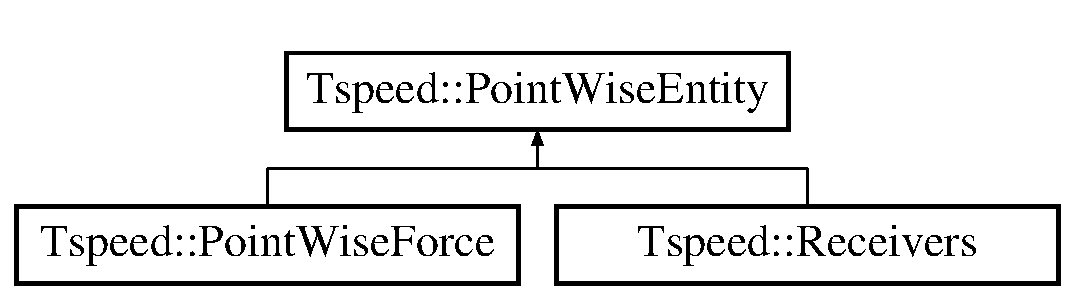
\includegraphics[height=2.000000cm]{classTspeed_1_1PointWiseEntity}
\end{center}
\end{figure}
\subsection*{Public Member Functions}
\begin{DoxyCompactItemize}
\item 
virtual \hyperlink{classTspeed_1_1PointWiseEntity_a602393b4fd96ffd3d40ea3ff30cdc366}{$\sim$\-Point\-Wise\-Entity} ()
\item 
Eigen\-::\-Array\-Xd const \& \hyperlink{classTspeed_1_1PointWiseEntity_a9369e650140e66a58e902ee752cf36ca}{shape} (int \hyperlink{vtk__vector__out_8m_a6f6ccfcf58b31cb6412107d9d5281426}{i}) const 
\item 
\hyperlink{classTspeed_1_1Geo_1_1Point}{Geo\-::\-Point} const \& \hyperlink{classTspeed_1_1PointWiseEntity_a4a71d4b7bfa160b2aaa6d3d2a4c35713}{point} (int \hyperlink{vtk__vector__out_8m_a6f6ccfcf58b31cb6412107d9d5281426}{i}) const 
\item 
unsigned int const \& \hyperlink{classTspeed_1_1PointWiseEntity_ac1271c51d7dd8689a38a60ca858e160f}{elem} (int \hyperlink{vtk__vector__out_8m_a6f6ccfcf58b31cb6412107d9d5281426}{i}) const 
\item 
unsigned int \hyperlink{classTspeed_1_1PointWiseEntity_aea02312bcb1b3c20a465e2d696b65924}{size} () const 
\end{DoxyCompactItemize}
\subsection*{Protected Member Functions}
\begin{DoxyCompactItemize}
\item 
{\footnotesize template$<$int N, typename Q , typename S $>$ }\\void \hyperlink{classTspeed_1_1PointWiseEntity_a8e8e5d0b5785b72de3b9f7ef1cbfcd81}{M\-\_\-add} (\hyperlink{namespaceTspeed_a05fcb57094666c8f5ab1e90d1a6fecf8}{F\-E\-Space\-\_\-ptr}$<$ N, Q, S $>$, \hyperlink{classTspeed_1_1Geo_1_1Point}{Geo\-::\-Point} const \&)
\end{DoxyCompactItemize}
\subsection*{Protected Attributes}
\begin{DoxyCompactItemize}
\item 
std\-::vector$<$ unsigned int $>$ \hyperlink{classTspeed_1_1PointWiseEntity_a46a04f3b7eac6a6bbe78fffe227116d2}{M\-\_\-ie}
\item 
std\-::vector$<$ \hyperlink{classTspeed_1_1Geo_1_1Point}{Geo\-::\-Point} $>$ \hyperlink{classTspeed_1_1PointWiseEntity_a7d32f8248f10ec3a0cf06bf41eeb5894}{M\-\_\-relp}
\item 
std\-::vector$<$ Eigen\-::\-Array\-Xd $>$ \hyperlink{classTspeed_1_1PointWiseEntity_a5be71b036f597e1a61909b1577ac2049}{M\-\_\-shape}
\item 
unsigned int \hyperlink{classTspeed_1_1PointWiseEntity_a054e68f482b69877a7a4c4d2b03d6db3}{M\-\_\-nel}
\end{DoxyCompactItemize}


\subsection{Constructor \& Destructor Documentation}
\hypertarget{classTspeed_1_1PointWiseEntity_a602393b4fd96ffd3d40ea3ff30cdc366}{\index{Tspeed\-::\-Point\-Wise\-Entity@{Tspeed\-::\-Point\-Wise\-Entity}!$\sim$\-Point\-Wise\-Entity@{$\sim$\-Point\-Wise\-Entity}}
\index{$\sim$\-Point\-Wise\-Entity@{$\sim$\-Point\-Wise\-Entity}!Tspeed::PointWiseEntity@{Tspeed\-::\-Point\-Wise\-Entity}}
\subsubsection[{$\sim$\-Point\-Wise\-Entity}]{\setlength{\rightskip}{0pt plus 5cm}virtual Tspeed\-::\-Point\-Wise\-Entity\-::$\sim$\-Point\-Wise\-Entity (
\begin{DoxyParamCaption}
{}
\end{DoxyParamCaption}
)\hspace{0.3cm}{\ttfamily [inline]}, {\ttfamily [virtual]}}}\label{classTspeed_1_1PointWiseEntity_a602393b4fd96ffd3d40ea3ff30cdc366}


\subsection{Member Function Documentation}
\hypertarget{classTspeed_1_1PointWiseEntity_ac1271c51d7dd8689a38a60ca858e160f}{\index{Tspeed\-::\-Point\-Wise\-Entity@{Tspeed\-::\-Point\-Wise\-Entity}!elem@{elem}}
\index{elem@{elem}!Tspeed::PointWiseEntity@{Tspeed\-::\-Point\-Wise\-Entity}}
\subsubsection[{elem}]{\setlength{\rightskip}{0pt plus 5cm}unsigned int const\& Tspeed\-::\-Point\-Wise\-Entity\-::elem (
\begin{DoxyParamCaption}
\item[{int}]{i}
\end{DoxyParamCaption}
) const\hspace{0.3cm}{\ttfamily [inline]}}}\label{classTspeed_1_1PointWiseEntity_ac1271c51d7dd8689a38a60ca858e160f}
\hypertarget{classTspeed_1_1PointWiseEntity_a8e8e5d0b5785b72de3b9f7ef1cbfcd81}{\index{Tspeed\-::\-Point\-Wise\-Entity@{Tspeed\-::\-Point\-Wise\-Entity}!M\-\_\-add@{M\-\_\-add}}
\index{M\-\_\-add@{M\-\_\-add}!Tspeed::PointWiseEntity@{Tspeed\-::\-Point\-Wise\-Entity}}
\subsubsection[{M\-\_\-add}]{\setlength{\rightskip}{0pt plus 5cm}template$<$int N, typename Q , typename S $>$ void Tspeed\-::\-Point\-Wise\-Entity\-::\-M\-\_\-add (
\begin{DoxyParamCaption}
\item[{{\bf F\-E\-Space\-\_\-ptr}$<$ N, Q, S $>$}]{Xh, }
\item[{{\bf Geo\-::\-Point} const \&}]{p}
\end{DoxyParamCaption}
)\hspace{0.3cm}{\ttfamily [protected]}}}\label{classTspeed_1_1PointWiseEntity_a8e8e5d0b5785b72de3b9f7ef1cbfcd81}
\hypertarget{classTspeed_1_1PointWiseEntity_a4a71d4b7bfa160b2aaa6d3d2a4c35713}{\index{Tspeed\-::\-Point\-Wise\-Entity@{Tspeed\-::\-Point\-Wise\-Entity}!point@{point}}
\index{point@{point}!Tspeed::PointWiseEntity@{Tspeed\-::\-Point\-Wise\-Entity}}
\subsubsection[{point}]{\setlength{\rightskip}{0pt plus 5cm}{\bf Geo\-::\-Point} const\& Tspeed\-::\-Point\-Wise\-Entity\-::point (
\begin{DoxyParamCaption}
\item[{int}]{i}
\end{DoxyParamCaption}
) const\hspace{0.3cm}{\ttfamily [inline]}}}\label{classTspeed_1_1PointWiseEntity_a4a71d4b7bfa160b2aaa6d3d2a4c35713}
\hypertarget{classTspeed_1_1PointWiseEntity_a9369e650140e66a58e902ee752cf36ca}{\index{Tspeed\-::\-Point\-Wise\-Entity@{Tspeed\-::\-Point\-Wise\-Entity}!shape@{shape}}
\index{shape@{shape}!Tspeed::PointWiseEntity@{Tspeed\-::\-Point\-Wise\-Entity}}
\subsubsection[{shape}]{\setlength{\rightskip}{0pt plus 5cm}Eigen\-::\-Array\-Xd const\& Tspeed\-::\-Point\-Wise\-Entity\-::shape (
\begin{DoxyParamCaption}
\item[{int}]{i}
\end{DoxyParamCaption}
) const\hspace{0.3cm}{\ttfamily [inline]}}}\label{classTspeed_1_1PointWiseEntity_a9369e650140e66a58e902ee752cf36ca}
\hypertarget{classTspeed_1_1PointWiseEntity_aea02312bcb1b3c20a465e2d696b65924}{\index{Tspeed\-::\-Point\-Wise\-Entity@{Tspeed\-::\-Point\-Wise\-Entity}!size@{size}}
\index{size@{size}!Tspeed::PointWiseEntity@{Tspeed\-::\-Point\-Wise\-Entity}}
\subsubsection[{size}]{\setlength{\rightskip}{0pt plus 5cm}unsigned int Tspeed\-::\-Point\-Wise\-Entity\-::size (
\begin{DoxyParamCaption}
{}
\end{DoxyParamCaption}
) const\hspace{0.3cm}{\ttfamily [inline]}}}\label{classTspeed_1_1PointWiseEntity_aea02312bcb1b3c20a465e2d696b65924}


\subsection{Member Data Documentation}
\hypertarget{classTspeed_1_1PointWiseEntity_a46a04f3b7eac6a6bbe78fffe227116d2}{\index{Tspeed\-::\-Point\-Wise\-Entity@{Tspeed\-::\-Point\-Wise\-Entity}!M\-\_\-ie@{M\-\_\-ie}}
\index{M\-\_\-ie@{M\-\_\-ie}!Tspeed::PointWiseEntity@{Tspeed\-::\-Point\-Wise\-Entity}}
\subsubsection[{M\-\_\-ie}]{\setlength{\rightskip}{0pt plus 5cm}std\-::vector$<$unsigned int$>$ Tspeed\-::\-Point\-Wise\-Entity\-::\-M\-\_\-ie\hspace{0.3cm}{\ttfamily [protected]}}}\label{classTspeed_1_1PointWiseEntity_a46a04f3b7eac6a6bbe78fffe227116d2}
\hypertarget{classTspeed_1_1PointWiseEntity_a054e68f482b69877a7a4c4d2b03d6db3}{\index{Tspeed\-::\-Point\-Wise\-Entity@{Tspeed\-::\-Point\-Wise\-Entity}!M\-\_\-nel@{M\-\_\-nel}}
\index{M\-\_\-nel@{M\-\_\-nel}!Tspeed::PointWiseEntity@{Tspeed\-::\-Point\-Wise\-Entity}}
\subsubsection[{M\-\_\-nel}]{\setlength{\rightskip}{0pt plus 5cm}unsigned int Tspeed\-::\-Point\-Wise\-Entity\-::\-M\-\_\-nel\hspace{0.3cm}{\ttfamily [protected]}}}\label{classTspeed_1_1PointWiseEntity_a054e68f482b69877a7a4c4d2b03d6db3}
\hypertarget{classTspeed_1_1PointWiseEntity_a7d32f8248f10ec3a0cf06bf41eeb5894}{\index{Tspeed\-::\-Point\-Wise\-Entity@{Tspeed\-::\-Point\-Wise\-Entity}!M\-\_\-relp@{M\-\_\-relp}}
\index{M\-\_\-relp@{M\-\_\-relp}!Tspeed::PointWiseEntity@{Tspeed\-::\-Point\-Wise\-Entity}}
\subsubsection[{M\-\_\-relp}]{\setlength{\rightskip}{0pt plus 5cm}std\-::vector$<${\bf Geo\-::\-Point}$>$ Tspeed\-::\-Point\-Wise\-Entity\-::\-M\-\_\-relp\hspace{0.3cm}{\ttfamily [protected]}}}\label{classTspeed_1_1PointWiseEntity_a7d32f8248f10ec3a0cf06bf41eeb5894}
\hypertarget{classTspeed_1_1PointWiseEntity_a5be71b036f597e1a61909b1577ac2049}{\index{Tspeed\-::\-Point\-Wise\-Entity@{Tspeed\-::\-Point\-Wise\-Entity}!M\-\_\-shape@{M\-\_\-shape}}
\index{M\-\_\-shape@{M\-\_\-shape}!Tspeed::PointWiseEntity@{Tspeed\-::\-Point\-Wise\-Entity}}
\subsubsection[{M\-\_\-shape}]{\setlength{\rightskip}{0pt plus 5cm}std\-::vector$<$Eigen\-::\-Array\-Xd$>$ Tspeed\-::\-Point\-Wise\-Entity\-::\-M\-\_\-shape\hspace{0.3cm}{\ttfamily [protected]}}}\label{classTspeed_1_1PointWiseEntity_a5be71b036f597e1a61909b1577ac2049}


The documentation for this class was generated from the following files\-:\begin{DoxyCompactItemize}
\item 
lib/include/\hyperlink{Receivers_8hpp}{Receivers.\-hpp}\item 
lib/include/\hyperlink{Receivers__imp_8hpp}{Receivers\-\_\-imp.\-hpp}\end{DoxyCompactItemize}

\hypertarget{classTspeed_1_1PointWiseForce}{\section{Tspeed\-:\-:Point\-Wise\-Force Class Reference}
\label{classTspeed_1_1PointWiseForce}\index{Tspeed\-::\-Point\-Wise\-Force@{Tspeed\-::\-Point\-Wise\-Force}}
}


{\ttfamily \#include $<$Force.\-hpp$>$}

Inheritance diagram for Tspeed\-:\-:Point\-Wise\-Force\-:\begin{figure}[H]
\begin{center}
\leavevmode
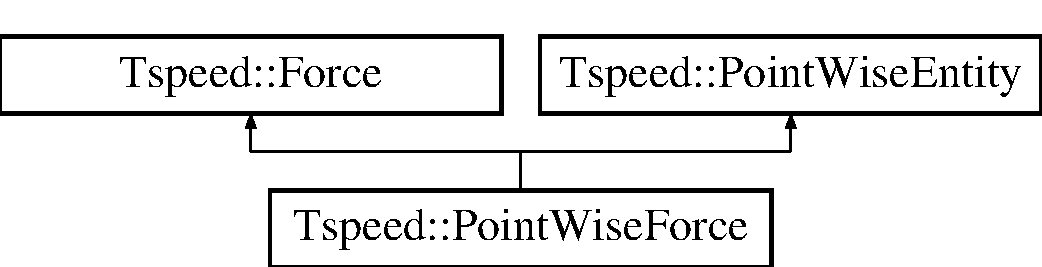
\includegraphics[height=2.000000cm]{classTspeed_1_1PointWiseForce}
\end{center}
\end{figure}
\subsection*{Public Member Functions}
\begin{DoxyCompactItemize}
\item 
{\footnotesize template$<$int N, typename Q , typename S $>$ }\\\hyperlink{classTspeed_1_1PointWiseForce_ad30aab53a735b22fac2b5cfeaa4d0c28}{Point\-Wise\-Force} (\hyperlink{vtk__vector__out_8m_a6235d6cebbf2f77ca6dbae2811d86530}{std\-::function}$<$ std\-::array$<$ double, 2 $>$(const double \&)$>$ const \&, \hyperlink{classTspeed_1_1Geo_1_1Point}{Geo\-::\-Point}, \hyperlink{namespaceTspeed_a05fcb57094666c8f5ab1e90d1a6fecf8}{F\-E\-Space\-\_\-ptr}$<$ N, Q, S $>$)
\item 
virtual \hyperlink{classTspeed_1_1PointWiseForce_a34ad80033ed1e9d5ba31feffae4ab7c9}{$\sim$\-Point\-Wise\-Force} ()
\item 
\hyperlink{classTspeed_1_1Force_ab33d4f6bed9bf9a136afd1ac5a918c93}{Vec} \hyperlink{classTspeed_1_1PointWiseForce_ae52b1302d87e4535620e205fe030d542}{eval} (const double \&) const 
\end{DoxyCompactItemize}
\subsection*{Additional Inherited Members}


\subsection{Constructor \& Destructor Documentation}
\hypertarget{classTspeed_1_1PointWiseForce_ad30aab53a735b22fac2b5cfeaa4d0c28}{\index{Tspeed\-::\-Point\-Wise\-Force@{Tspeed\-::\-Point\-Wise\-Force}!Point\-Wise\-Force@{Point\-Wise\-Force}}
\index{Point\-Wise\-Force@{Point\-Wise\-Force}!Tspeed::PointWiseForce@{Tspeed\-::\-Point\-Wise\-Force}}
\subsubsection[{Point\-Wise\-Force}]{\setlength{\rightskip}{0pt plus 5cm}template$<$int N, typename Q , typename S $>$ Tspeed\-::\-Point\-Wise\-Force\-::\-Point\-Wise\-Force (
\begin{DoxyParamCaption}
\item[{{\bf std\-::function}$<$ std\-::array$<$ double, 2 $>$(const double \&)$>$ const \&}]{f, }
\item[{{\bf Geo\-::\-Point}}]{p, }
\item[{{\bf F\-E\-Space\-\_\-ptr}$<$ N, Q, S $>$}]{Xh}
\end{DoxyParamCaption}
)}}\label{classTspeed_1_1PointWiseForce_ad30aab53a735b22fac2b5cfeaa4d0c28}
\hypertarget{classTspeed_1_1PointWiseForce_a34ad80033ed1e9d5ba31feffae4ab7c9}{\index{Tspeed\-::\-Point\-Wise\-Force@{Tspeed\-::\-Point\-Wise\-Force}!$\sim$\-Point\-Wise\-Force@{$\sim$\-Point\-Wise\-Force}}
\index{$\sim$\-Point\-Wise\-Force@{$\sim$\-Point\-Wise\-Force}!Tspeed::PointWiseForce@{Tspeed\-::\-Point\-Wise\-Force}}
\subsubsection[{$\sim$\-Point\-Wise\-Force}]{\setlength{\rightskip}{0pt plus 5cm}virtual Tspeed\-::\-Point\-Wise\-Force\-::$\sim$\-Point\-Wise\-Force (
\begin{DoxyParamCaption}
{}
\end{DoxyParamCaption}
)\hspace{0.3cm}{\ttfamily [inline]}, {\ttfamily [virtual]}}}\label{classTspeed_1_1PointWiseForce_a34ad80033ed1e9d5ba31feffae4ab7c9}


\subsection{Member Function Documentation}
\hypertarget{classTspeed_1_1PointWiseForce_ae52b1302d87e4535620e205fe030d542}{\index{Tspeed\-::\-Point\-Wise\-Force@{Tspeed\-::\-Point\-Wise\-Force}!eval@{eval}}
\index{eval@{eval}!Tspeed::PointWiseForce@{Tspeed\-::\-Point\-Wise\-Force}}
\subsubsection[{eval}]{\setlength{\rightskip}{0pt plus 5cm}Eigen\-::\-Vector\-Xd Tspeed\-::\-Point\-Wise\-Force\-::eval (
\begin{DoxyParamCaption}
\item[{const double \&}]{t}
\end{DoxyParamCaption}
) const\hspace{0.3cm}{\ttfamily [virtual]}}}\label{classTspeed_1_1PointWiseForce_ae52b1302d87e4535620e205fe030d542}


Implements \hyperlink{classTspeed_1_1Force_ac174525b11c7c6a490411d00330a3564}{Tspeed\-::\-Force}.



The documentation for this class was generated from the following files\-:\begin{DoxyCompactItemize}
\item 
lib/include/\hyperlink{Force_8hpp}{Force.\-hpp}\item 
lib/include/\hyperlink{Force__imp_8hpp}{Force\-\_\-imp.\-hpp}\item 
lib/src/\hyperlink{Force_8cpp}{Force.\-cpp}\end{DoxyCompactItemize}

\hypertarget{classTspeed_1_1Receivers}{\section{Tspeed\-:\-:Receivers Class Reference}
\label{classTspeed_1_1Receivers}\index{Tspeed\-::\-Receivers@{Tspeed\-::\-Receivers}}
}


{\ttfamily \#include $<$Receivers.\-hpp$>$}

Inheritance diagram for Tspeed\-:\-:Receivers\-:\begin{figure}[H]
\begin{center}
\leavevmode
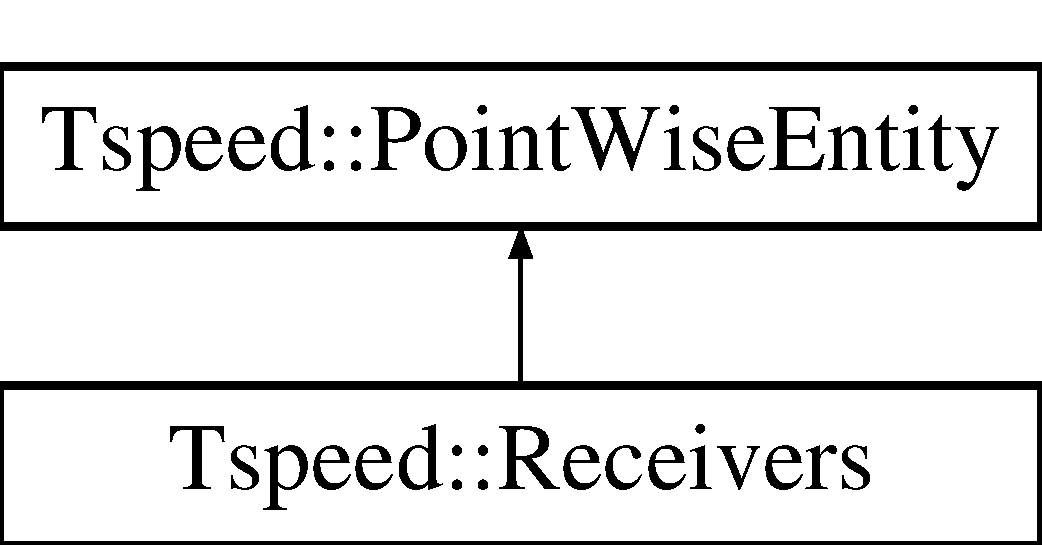
\includegraphics[height=2.000000cm]{classTspeed_1_1Receivers}
\end{center}
\end{figure}
\subsection*{Public Member Functions}
\begin{DoxyCompactItemize}
\item 
{\footnotesize template$<$int N, typename Q , typename S $>$ }\\\hyperlink{classTspeed_1_1Receivers_a54d8209b84f325fbf6470318cd961e76}{Receivers} (\hyperlink{namespaceTspeed_a05fcb57094666c8f5ab1e90d1a6fecf8}{F\-E\-Space\-\_\-ptr}$<$ N, Q, S $>$, std\-::string const \&)
\item 
{\footnotesize template$<$int N, typename Q , typename S $>$ }\\\hyperlink{classTspeed_1_1Receivers_a70779bee95d94ef96f416deabc4f42c8}{Receivers} (\hyperlink{namespaceTspeed_a05fcb57094666c8f5ab1e90d1a6fecf8}{F\-E\-Space\-\_\-ptr}$<$ N, Q, S $>$, \hyperlink{classTspeed_1_1Geo_1_1Point}{Geo\-::\-Point} const \&)
\item 
void \hyperlink{classTspeed_1_1Receivers_a6048d3823edb7ed2481ed8c50fedca10}{add} (double const \&\hyperlink{vtk__mesh__out_8m_ace4b66138f2e64832c951b1ba9ce24cc}{x}, double const \&\hyperlink{vtk__mesh__out_8m_a2fb1c5cf58867b5bbc9a1b145a86f3a0}{y}, unsigned int const \&, unsigned int const \&)
\item 
void \hyperlink{classTspeed_1_1Receivers_acd4b059932051140166eb0592fb0223a}{write} (std\-::string const \&) const 
\end{DoxyCompactItemize}
\subsection*{Additional Inherited Members}


\subsection{Constructor \& Destructor Documentation}
\hypertarget{classTspeed_1_1Receivers_a54d8209b84f325fbf6470318cd961e76}{\index{Tspeed\-::\-Receivers@{Tspeed\-::\-Receivers}!Receivers@{Receivers}}
\index{Receivers@{Receivers}!Tspeed::Receivers@{Tspeed\-::\-Receivers}}
\subsubsection[{Receivers}]{\setlength{\rightskip}{0pt plus 5cm}template$<$int N, typename Q , typename S $>$ Tspeed\-::\-Receivers\-::\-Receivers (
\begin{DoxyParamCaption}
\item[{{\bf F\-E\-Space\-\_\-ptr}$<$ N, Q, S $>$}]{Xh, }
\item[{std\-::string const \&}]{fname}
\end{DoxyParamCaption}
)}}\label{classTspeed_1_1Receivers_a54d8209b84f325fbf6470318cd961e76}
\hypertarget{classTspeed_1_1Receivers_a70779bee95d94ef96f416deabc4f42c8}{\index{Tspeed\-::\-Receivers@{Tspeed\-::\-Receivers}!Receivers@{Receivers}}
\index{Receivers@{Receivers}!Tspeed::Receivers@{Tspeed\-::\-Receivers}}
\subsubsection[{Receivers}]{\setlength{\rightskip}{0pt plus 5cm}template$<$int N, typename Q , typename S $>$ Tspeed\-::\-Receivers\-::\-Receivers (
\begin{DoxyParamCaption}
\item[{{\bf F\-E\-Space\-\_\-ptr}$<$ N, Q, S $>$}]{Xh, }
\item[{{\bf Geo\-::\-Point} const \&}]{p}
\end{DoxyParamCaption}
)}}\label{classTspeed_1_1Receivers_a70779bee95d94ef96f416deabc4f42c8}


\subsection{Member Function Documentation}
\hypertarget{classTspeed_1_1Receivers_a6048d3823edb7ed2481ed8c50fedca10}{\index{Tspeed\-::\-Receivers@{Tspeed\-::\-Receivers}!add@{add}}
\index{add@{add}!Tspeed::Receivers@{Tspeed\-::\-Receivers}}
\subsubsection[{add}]{\setlength{\rightskip}{0pt plus 5cm}void Tspeed\-::\-Receivers\-::add (
\begin{DoxyParamCaption}
\item[{double const \&}]{x, }
\item[{double const \&}]{y, }
\item[{unsigned int const \&}]{ir, }
\item[{unsigned int const \&}]{step}
\end{DoxyParamCaption}
)}}\label{classTspeed_1_1Receivers_a6048d3823edb7ed2481ed8c50fedca10}
\hypertarget{classTspeed_1_1Receivers_acd4b059932051140166eb0592fb0223a}{\index{Tspeed\-::\-Receivers@{Tspeed\-::\-Receivers}!write@{write}}
\index{write@{write}!Tspeed::Receivers@{Tspeed\-::\-Receivers}}
\subsubsection[{write}]{\setlength{\rightskip}{0pt plus 5cm}void Tspeed\-::\-Receivers\-::write (
\begin{DoxyParamCaption}
\item[{std\-::string const \&}]{fn}
\end{DoxyParamCaption}
) const}}\label{classTspeed_1_1Receivers_acd4b059932051140166eb0592fb0223a}


The documentation for this class was generated from the following files\-:\begin{DoxyCompactItemize}
\item 
lib/include/\hyperlink{Receivers_8hpp}{Receivers.\-hpp}\item 
lib/include/\hyperlink{Receivers__imp_8hpp}{Receivers\-\_\-imp.\-hpp}\item 
lib/src/\hyperlink{Receivers_8cpp}{Receivers.\-cpp}\end{DoxyCompactItemize}

\hypertarget{classTspeed_1_1ShapeFunction}{\section{Tspeed\-:\-:Shape\-Function$<$ N $>$ Class Template Reference}
\label{classTspeed_1_1ShapeFunction}\index{Tspeed\-::\-Shape\-Function$<$ N $>$@{Tspeed\-::\-Shape\-Function$<$ N $>$}}
}


Base class for the shared functions.  




{\ttfamily \#include $<$Shape\-Functions.\-hpp$>$}

Inheritance diagram for Tspeed\-:\-:Shape\-Function$<$ N $>$\-:\begin{figure}[H]
\begin{center}
\leavevmode
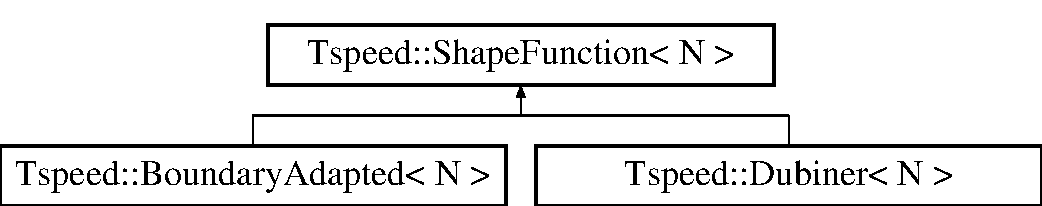
\includegraphics[height=2.000000cm]{classTspeed_1_1ShapeFunction}
\end{center}
\end{figure}
\subsection*{Public Types}
\begin{DoxyCompactItemize}
\item 
enum \{ \hyperlink{classTspeed_1_1ShapeFunction_aae4b82bb304115736483f3549b135662a5000f7869288e4deef5af90732ca04fc}{gdl} = (N+1)$\ast$(N+2)/2
 \}
\begin{DoxyCompactList}\small\item\em Number of degrees of freedom. \end{DoxyCompactList}\item 
enum \{ \hyperlink{classTspeed_1_1ShapeFunction_ab93d04cd0692e117dffed761620d57c1a62f499700236320c9364d9c4bc9ab564}{is\-\_\-orthonormal} = false
 \}
\begin{DoxyCompactList}\small\item\em Orthonormality of the basis. \end{DoxyCompactList}\end{DoxyCompactItemize}
\subsection*{Public Member Functions}
\begin{DoxyCompactItemize}
\item 
virtual \hyperlink{classTspeed_1_1ShapeFunction_abfab4ad1f425751c62102f74f6ff8040}{$\sim$\-Shape\-Function} ()
\item 
\hyperlink{classTspeed_1_1ShapeFunction_ad445923bd9ccbd1c50580f43a6342f5c}{Shape\-Function} ()
\item 
Eigen\-::\-Array\-Xd \hyperlink{classTspeed_1_1ShapeFunction_a30886f42b86096f6ea4b621cd4255dd1}{phi} (unsigned int s, Arr const \&v, Arr const \&w) const 
\begin{DoxyCompactList}\small\item\em Get value of base function with index s, on points (v,w) \end{DoxyCompactList}\item 
double \hyperlink{classTspeed_1_1ShapeFunction_a45ca655484d81ea09b474ae628d79ecf}{phi} (unsigned int s, double x, double y) const 
\begin{DoxyCompactList}\small\item\em Get value of base function with index s, on point (x,y) \end{DoxyCompactList}\item 
Arr\-G \hyperlink{classTspeed_1_1ShapeFunction_aac13d9c4a86f3a2f9b188a199676c2da}{grad} (unsigned int s, Arr const \&v, Arr const \&w)
\begin{DoxyCompactList}\small\item\em Get values of gradient of basis function s, on points (v,w) \end{DoxyCompactList}\end{DoxyCompactItemize}
\subsection*{Protected Attributes}
\begin{DoxyCompactItemize}
\item 
std\-::vector$<$ std\-::function\\*
$<$ Arr(Arr const \&, Arr const \&)$>$ $>$ \hyperlink{classTspeed_1_1ShapeFunction_a6d8010d0c9d5e40f21f57c8201149ad5}{M\-\_\-phi}
\item 
std\-::vector$<$ std\-::function\\*
$<$ Arr\-G(Arr const \&, Arr const \&)$>$ $>$ \hyperlink{classTspeed_1_1ShapeFunction_a282cf4ac589829f07a6c24e443d7bd05}{M\-\_\-grad}
\end{DoxyCompactItemize}


\subsection{Detailed Description}
\subsubsection*{template$<$int N$>$class Tspeed\-::\-Shape\-Function$<$ N $>$}

Base class for the shared functions. 


\begin{DoxyTemplParams}{Template Parameters}
{\em N} & degree of the space $\mathbb{P}_N$ \\
\hline
\end{DoxyTemplParams}


\subsection{Member Enumeration Documentation}
\hypertarget{classTspeed_1_1ShapeFunction_aae4b82bb304115736483f3549b135662}{\subsubsection[{anonymous enum}]{\setlength{\rightskip}{0pt plus 5cm}template$<$int N$>$ anonymous enum}}\label{classTspeed_1_1ShapeFunction_aae4b82bb304115736483f3549b135662}


Number of degrees of freedom. 

\begin{Desc}
\item[Enumerator]\par
\begin{description}
\index{gdl@{gdl}!Tspeed\-::\-Shape\-Function@{Tspeed\-::\-Shape\-Function}}\index{Tspeed\-::\-Shape\-Function@{Tspeed\-::\-Shape\-Function}!gdl@{gdl}}\item[{\em 
\hypertarget{classTspeed_1_1ShapeFunction_aae4b82bb304115736483f3549b135662a5000f7869288e4deef5af90732ca04fc}{gdl}\label{classTspeed_1_1ShapeFunction_aae4b82bb304115736483f3549b135662a5000f7869288e4deef5af90732ca04fc}
}]\end{description}
\end{Desc}
\hypertarget{classTspeed_1_1ShapeFunction_ab93d04cd0692e117dffed761620d57c1}{\subsubsection[{anonymous enum}]{\setlength{\rightskip}{0pt plus 5cm}template$<$int N$>$ anonymous enum}}\label{classTspeed_1_1ShapeFunction_ab93d04cd0692e117dffed761620d57c1}


Orthonormality of the basis. 

\begin{Desc}
\item[Enumerator]\par
\begin{description}
\index{is\-\_\-orthonormal@{is\-\_\-orthonormal}!Tspeed\-::\-Shape\-Function@{Tspeed\-::\-Shape\-Function}}\index{Tspeed\-::\-Shape\-Function@{Tspeed\-::\-Shape\-Function}!is\-\_\-orthonormal@{is\-\_\-orthonormal}}\item[{\em 
\hypertarget{classTspeed_1_1ShapeFunction_ab93d04cd0692e117dffed761620d57c1a62f499700236320c9364d9c4bc9ab564}{is\-\_\-orthonormal}\label{classTspeed_1_1ShapeFunction_ab93d04cd0692e117dffed761620d57c1a62f499700236320c9364d9c4bc9ab564}
}]\end{description}
\end{Desc}


\subsection{Constructor \& Destructor Documentation}
\hypertarget{classTspeed_1_1ShapeFunction_abfab4ad1f425751c62102f74f6ff8040}{\index{Tspeed\-::\-Shape\-Function@{Tspeed\-::\-Shape\-Function}!$\sim$\-Shape\-Function@{$\sim$\-Shape\-Function}}
\index{$\sim$\-Shape\-Function@{$\sim$\-Shape\-Function}!Tspeed::ShapeFunction@{Tspeed\-::\-Shape\-Function}}
\subsubsection[{$\sim$\-Shape\-Function}]{\setlength{\rightskip}{0pt plus 5cm}template$<$int N$>$ virtual {\bf Tspeed\-::\-Shape\-Function}$<$ N $>$\-::$\sim${\bf Shape\-Function} (
\begin{DoxyParamCaption}
{}
\end{DoxyParamCaption}
)\hspace{0.3cm}{\ttfamily [inline]}, {\ttfamily [virtual]}}}\label{classTspeed_1_1ShapeFunction_abfab4ad1f425751c62102f74f6ff8040}
\hypertarget{classTspeed_1_1ShapeFunction_ad445923bd9ccbd1c50580f43a6342f5c}{\index{Tspeed\-::\-Shape\-Function@{Tspeed\-::\-Shape\-Function}!Shape\-Function@{Shape\-Function}}
\index{Shape\-Function@{Shape\-Function}!Tspeed::ShapeFunction@{Tspeed\-::\-Shape\-Function}}
\subsubsection[{Shape\-Function}]{\setlength{\rightskip}{0pt plus 5cm}template$<$int N$>$ {\bf Tspeed\-::\-Shape\-Function}$<$ N $>$\-::{\bf Shape\-Function} (
\begin{DoxyParamCaption}
{}
\end{DoxyParamCaption}
)\hspace{0.3cm}{\ttfamily [inline]}}}\label{classTspeed_1_1ShapeFunction_ad445923bd9ccbd1c50580f43a6342f5c}


\subsection{Member Function Documentation}
\hypertarget{classTspeed_1_1ShapeFunction_aac13d9c4a86f3a2f9b188a199676c2da}{\index{Tspeed\-::\-Shape\-Function@{Tspeed\-::\-Shape\-Function}!grad@{grad}}
\index{grad@{grad}!Tspeed::ShapeFunction@{Tspeed\-::\-Shape\-Function}}
\subsubsection[{grad}]{\setlength{\rightskip}{0pt plus 5cm}template$<$int N$>$ Arr\-G {\bf Tspeed\-::\-Shape\-Function}$<$ N $>$\-::grad (
\begin{DoxyParamCaption}
\item[{unsigned int}]{s, }
\item[{Arr const \&}]{v, }
\item[{Arr const \&}]{w}
\end{DoxyParamCaption}
)\hspace{0.3cm}{\ttfamily [inline]}}}\label{classTspeed_1_1ShapeFunction_aac13d9c4a86f3a2f9b188a199676c2da}


Get values of gradient of basis function s, on points (v,w) 


\begin{DoxyParams}{Parameters}
{\em s} & Index f the function \\
\hline
{\em v} & x-\/coordinates of the points \\
\hline
{\em w} & y-\/coordinates of the points\\
\hline
\end{DoxyParams}
\begin{DoxyReturn}{Returns}
An array of dimension length(v) , 2 with the values 
\end{DoxyReturn}
\hypertarget{classTspeed_1_1ShapeFunction_a30886f42b86096f6ea4b621cd4255dd1}{\index{Tspeed\-::\-Shape\-Function@{Tspeed\-::\-Shape\-Function}!phi@{phi}}
\index{phi@{phi}!Tspeed::ShapeFunction@{Tspeed\-::\-Shape\-Function}}
\subsubsection[{phi}]{\setlength{\rightskip}{0pt plus 5cm}template$<$int N$>$ Eigen\-::\-Array\-Xd {\bf Tspeed\-::\-Shape\-Function}$<$ N $>$\-::phi (
\begin{DoxyParamCaption}
\item[{unsigned int}]{s, }
\item[{Arr const \&}]{v, }
\item[{Arr const \&}]{w}
\end{DoxyParamCaption}
) const\hspace{0.3cm}{\ttfamily [inline]}}}\label{classTspeed_1_1ShapeFunction_a30886f42b86096f6ea4b621cd4255dd1}


Get value of base function with index s, on points (v,w) 


\begin{DoxyParams}{Parameters}
{\em s} & index of the basis function \\
\hline
{\em v} & x-\/coordinates of the points \\
\hline
{\em w} & y-\/coordinates of the points\\
\hline
\end{DoxyParams}
\begin{DoxyReturn}{Returns}
An Eigen array with the values 
\end{DoxyReturn}
\hypertarget{classTspeed_1_1ShapeFunction_a45ca655484d81ea09b474ae628d79ecf}{\index{Tspeed\-::\-Shape\-Function@{Tspeed\-::\-Shape\-Function}!phi@{phi}}
\index{phi@{phi}!Tspeed::ShapeFunction@{Tspeed\-::\-Shape\-Function}}
\subsubsection[{phi}]{\setlength{\rightskip}{0pt plus 5cm}template$<$int N$>$ double {\bf Tspeed\-::\-Shape\-Function}$<$ N $>$\-::phi (
\begin{DoxyParamCaption}
\item[{unsigned int}]{s, }
\item[{double}]{x, }
\item[{double}]{y}
\end{DoxyParamCaption}
) const\hspace{0.3cm}{\ttfamily [inline]}}}\label{classTspeed_1_1ShapeFunction_a45ca655484d81ea09b474ae628d79ecf}


Get value of base function with index s, on point (x,y) 


\begin{DoxyParams}{Parameters}
{\em s} & index of the basis function \\
\hline
{\em x} & x-\/coordinates of the point \\
\hline
{\em y} & y-\/coordinates of the point\\
\hline
\end{DoxyParams}
\begin{DoxyReturn}{Returns}
the value 
\end{DoxyReturn}


\subsection{Member Data Documentation}
\hypertarget{classTspeed_1_1ShapeFunction_a282cf4ac589829f07a6c24e443d7bd05}{\index{Tspeed\-::\-Shape\-Function@{Tspeed\-::\-Shape\-Function}!M\-\_\-grad@{M\-\_\-grad}}
\index{M\-\_\-grad@{M\-\_\-grad}!Tspeed::ShapeFunction@{Tspeed\-::\-Shape\-Function}}
\subsubsection[{M\-\_\-grad}]{\setlength{\rightskip}{0pt plus 5cm}template$<$int N$>$ std\-::vector$<$std\-::function$<$Arr\-G(Arr const \&, Arr const \&)$>$ $>$ {\bf Tspeed\-::\-Shape\-Function}$<$ N $>$\-::M\-\_\-grad\hspace{0.3cm}{\ttfamily [protected]}}}\label{classTspeed_1_1ShapeFunction_a282cf4ac589829f07a6c24e443d7bd05}
\hypertarget{classTspeed_1_1ShapeFunction_a6d8010d0c9d5e40f21f57c8201149ad5}{\index{Tspeed\-::\-Shape\-Function@{Tspeed\-::\-Shape\-Function}!M\-\_\-phi@{M\-\_\-phi}}
\index{M\-\_\-phi@{M\-\_\-phi}!Tspeed::ShapeFunction@{Tspeed\-::\-Shape\-Function}}
\subsubsection[{M\-\_\-phi}]{\setlength{\rightskip}{0pt plus 5cm}template$<$int N$>$ std\-::vector$<$std\-::function$<$Arr(Arr const \&, Arr const \&)$>$ $>$ {\bf Tspeed\-::\-Shape\-Function}$<$ N $>$\-::M\-\_\-phi\hspace{0.3cm}{\ttfamily [protected]}}}\label{classTspeed_1_1ShapeFunction_a6d8010d0c9d5e40f21f57c8201149ad5}


The documentation for this class was generated from the following file\-:\begin{DoxyCompactItemize}
\item 
lib/include/\hyperlink{ShapeFunctions_8hpp}{Shape\-Functions.\-hpp}\end{DoxyCompactItemize}

\hypertarget{classTspeed_1_1TimeAdvance}{\section{Tspeed\-:\-:Time\-Advance Class Reference}
\label{classTspeed_1_1TimeAdvance}\index{Tspeed\-::\-Time\-Advance@{Tspeed\-::\-Time\-Advance}}
}


Base class for time stepping methods.  




{\ttfamily \#include $<$Time\-Advance.\-hpp$>$}

Inheritance diagram for Tspeed\-:\-:Time\-Advance\-:\begin{figure}[H]
\begin{center}
\leavevmode
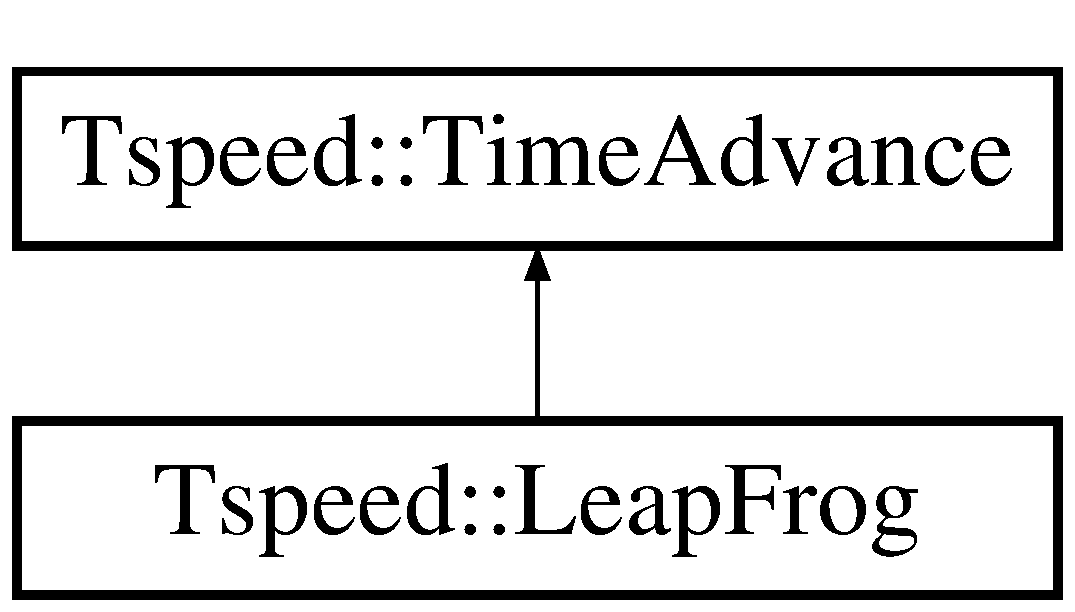
\includegraphics[height=2.000000cm]{classTspeed_1_1TimeAdvance}
\end{center}
\end{figure}
\subsection*{Public Member Functions}
\begin{DoxyCompactItemize}
\item 
{\footnotesize template$<$int N, typename Q , typename S $>$ }\\\hyperlink{classTspeed_1_1TimeAdvance_ab7fb5289ea62abe7da6c4423bf19f667}{Time\-Advance} (\hyperlink{namespaceTspeed_a05fcb57094666c8f5ab1e90d1a6fecf8}{F\-E\-Space\-\_\-ptr}$<$ N, Q, S $>$ Xh, \hyperlink{classTspeed_1_1Parameters}{Parameters} const \&p, \hyperlink{classTspeed_1_1Receivers}{Receivers} const \&r)
\begin{DoxyCompactList}\small\item\em constructor from the space, parameters and receivers \end{DoxyCompactList}\item 
void \hyperlink{classTspeed_1_1TimeAdvance_ae9d353495c283af5a29740a70424f11d}{first\-\_\-step} ()
\begin{DoxyCompactList}\small\item\em The first step of the method (which is different for 2nd order methods) \end{DoxyCompactList}\item 
void \hyperlink{classTspeed_1_1TimeAdvance_a3328d4d45d9261de6bfdd8e447f88d63}{step} (double t)
\begin{DoxyCompactList}\small\item\em step at time t \end{DoxyCompactList}\item 
virtual \hyperlink{classTspeed_1_1TimeAdvance_a73dfdea3bdb8e9f33e7223399ac9f14c}{$\sim$\-Time\-Advance} ()
\item 
void \hyperlink{classTspeed_1_1TimeAdvance_a2538fb7b6ee62103de78f42158bf38e6}{set\-\_\-dt} (double dt)
\begin{DoxyCompactList}\small\item\em Set time step $\delta t $. \end{DoxyCompactList}\item 
void \hyperlink{classTspeed_1_1TimeAdvance_ac0d8cd9b2b704e7cd4a2dd0793ce085d}{set\-\_\-tmax} (double tmax)
\begin{DoxyCompactList}\small\item\em Set end time of the simulation. \end{DoxyCompactList}\item 
void \hyperlink{classTspeed_1_1TimeAdvance_af635a6b3e94ff39467817c4b3890feb4}{set\-\_\-penalty} (double p)
\begin{DoxyCompactList}\small\item\em set penalty for the stability matrix \end{DoxyCompactList}\item 
void \hyperlink{classTspeed_1_1TimeAdvance_a248fe5d89a8bff234c84bac80ed31adf}{add\-\_\-force} (std\-::shared\-\_\-ptr$<$ \hyperlink{classTspeed_1_1Force}{Force} $>$ \hyperlink{classTspeed_1_1TimeAdvance_a36dea2ae6ba03546806bbacb83697c01}{f})
\begin{DoxyCompactList}\small\item\em Add the force. \end{DoxyCompactList}\item 
{\footnotesize template$<$int N, typename Q , typename S $>$ }\\void \hyperlink{classTspeed_1_1TimeAdvance_a5565d8938d39054dbceae8b5fb26f6bc}{set\-\_\-initial\-\_\-v} (\hyperlink{namespaceTspeed_a05fcb57094666c8f5ab1e90d1a6fecf8}{F\-E\-Space\-\_\-ptr}$<$ N, Q, S $>$ Xh, std\-::function$<$ std\-::array$<$ double, 2 $>$(double, double)$>$ fun)
\begin{DoxyCompactList}\small\item\em Set initial speed $ \dot{u} $. \end{DoxyCompactList}\item 
{\footnotesize template$<$int N, typename Q , typename S $>$ }\\void \hyperlink{classTspeed_1_1TimeAdvance_a458fb8edb53992055aceb6fee44f506a}{set\-\_\-initial\-\_\-u} (\hyperlink{namespaceTspeed_a05fcb57094666c8f5ab1e90d1a6fecf8}{F\-E\-Space\-\_\-ptr}$<$ N, Q, S $>$ Xh, std\-::function$<$ std\-::array$<$ double, 2 $>$(double, double)$>$ fun)
\begin{DoxyCompactList}\small\item\em Set initial displacement $ {u} $. \end{DoxyCompactList}\item 
bool \hyperlink{classTspeed_1_1TimeAdvance_a31398b7880b86622ba3c1378e2ac91d1}{is\-\_\-running} ()
\begin{DoxyCompactList}\small\item\em Check if the method has arrived at the final time. \end{DoxyCompactList}\item 
Vec const \& \hyperlink{classTspeed_1_1TimeAdvance_a3b4a0ed12f2fea72ce004dcdf467f10a}{get\-\_\-uh} () const 
\begin{DoxyCompactList}\small\item\em Get the coefficients of the numerical solution $u_h$. \end{DoxyCompactList}\item 
Vec const \& \hyperlink{classTspeed_1_1TimeAdvance_a3c27a46c3be458c4c6b9b7802c58a30b}{u} () const 
\item 
void \hyperlink{classTspeed_1_1TimeAdvance_aa4b4c155a949f5629e49da06a13e2672}{eval\-\_\-receivers} ()
\begin{DoxyCompactList}\small\item\em Compute and store the value of the displacement at the receivers. \end{DoxyCompactList}\item 
void \hyperlink{classTspeed_1_1TimeAdvance_a4030ab6e3606e5b762d236a4bc65fe68}{write\-\_\-receivers} (std\-::string const \&fn) const 
\begin{DoxyCompactList}\small\item\em Write the time series of the displacement at the receivers. \end{DoxyCompactList}\end{DoxyCompactItemize}
\subsection*{Protected Member Functions}
\begin{DoxyCompactItemize}
\item 
void \hyperlink{classTspeed_1_1TimeAdvance_ac083260ffe62e2a3eff1c1ab6068a1ad}{update\-\_\-variables} (double t)
\end{DoxyCompactItemize}
\subsection*{Protected Attributes}
\begin{DoxyCompactItemize}
\item 
double \hyperlink{classTspeed_1_1TimeAdvance_a153eb7bdf6d8034242dacdd3cdbf9950}{M\-\_\-penalty}
\item 
double \hyperlink{classTspeed_1_1TimeAdvance_aa1397f45ca8bcebaf879ca5e98d9daca}{M\-\_\-dt}
\item 
double \hyperlink{classTspeed_1_1TimeAdvance_a935eb9282bdd63bf94190f209a58756a}{M\-\_\-tmax}
\item 
Vec \hyperlink{classTspeed_1_1TimeAdvance_a36dea2ae6ba03546806bbacb83697c01}{f}
\item 
Vec \hyperlink{classTspeed_1_1TimeAdvance_a3cfbea04f0116183c5ac4ec59282d3e8}{fold}
\item 
Vec \hyperlink{classTspeed_1_1TimeAdvance_aac8169dc52fa2b5f00c87328707b9b26}{foldold}
\item 
Vec \hyperlink{classTspeed_1_1TimeAdvance_ab453aee6ca36887379834a7a228989d0}{uh}
\item 
Vec \hyperlink{classTspeed_1_1TimeAdvance_a5b8df69f25e0c457f1e6d1c7c6ed77e2}{uhold}
\item 
Vec \hyperlink{classTspeed_1_1TimeAdvance_a226deb2e9c8d165ad896bceb92c1330c}{uholdold}
\item 
Vec \hyperlink{classTspeed_1_1TimeAdvance_a981832947c160ad5471d63de23a37829}{initial\-\_\-v}
\item 
\hyperlink{classTspeed_1_1Receivers}{Receivers} \hyperlink{classTspeed_1_1TimeAdvance_a5e1ffc2d89b385049c83b446101ecca7}{M\-\_\-recv}
\item 
\hyperlink{classTspeed_1_1Matrices}{Matrices} \hyperlink{classTspeed_1_1TimeAdvance_aa8716f36ac9a3e725d9a2343e25efec3}{M\-\_\-mat}
\item 
\hyperlink{classTspeed_1_1MyMatMultiDim}{My\-Mat\-Multi\-Dim}$<$ \hyperlink{classTspeed_1_1MyMat}{My\-Mat} $>$ \hyperlink{classTspeed_1_1TimeAdvance_a10e673f4de9933dec049cb65261314ad}{B}
\item 
std\-::shared\-\_\-ptr$<$ \hyperlink{classTspeed_1_1Force}{Force} $>$ \hyperlink{classTspeed_1_1TimeAdvance_a2680ceda17b7629d86a866ab0e4754a6}{M\-\_\-f}
\item 
bool \hyperlink{classTspeed_1_1TimeAdvance_a7a14b1e98e28bded2816b27dabf44cb7}{M\-\_\-completed}
\item 
double \hyperlink{classTspeed_1_1TimeAdvance_a70a2f155f8dffcf2147ed52d208188f7}{M\-\_\-last\-\_\-step}
\item 
unsigned int \hyperlink{classTspeed_1_1TimeAdvance_a6ec24e3069ed3b6aa51af9ca09e9f727}{M\-\_\-recv\-\_\-written}
\item 
unsigned int \hyperlink{classTspeed_1_1TimeAdvance_a6c74b64240341a94c1e10b1bb9d20ae3}{M\-\_\-nln}
\item 
unsigned int \hyperlink{classTspeed_1_1TimeAdvance_aa03110e12846960054b42b4cf0d05b54}{M\-\_\-ne}
\end{DoxyCompactItemize}


\subsection{Detailed Description}
Base class for time stepping methods. 

\subsection{Constructor \& Destructor Documentation}
\hypertarget{classTspeed_1_1TimeAdvance_ab7fb5289ea62abe7da6c4423bf19f667}{\index{Tspeed\-::\-Time\-Advance@{Tspeed\-::\-Time\-Advance}!Time\-Advance@{Time\-Advance}}
\index{Time\-Advance@{Time\-Advance}!Tspeed::TimeAdvance@{Tspeed\-::\-Time\-Advance}}
\subsubsection[{Time\-Advance}]{\setlength{\rightskip}{0pt plus 5cm}template$<$int N, typename Q , typename S $>$ Tspeed\-::\-Time\-Advance\-::\-Time\-Advance (
\begin{DoxyParamCaption}
\item[{{\bf F\-E\-Space\-\_\-ptr}$<$ N, Q, S $>$}]{Xh, }
\item[{{\bf Parameters} const \&}]{p, }
\item[{{\bf Receivers} const \&}]{r}
\end{DoxyParamCaption}
)}}\label{classTspeed_1_1TimeAdvance_ab7fb5289ea62abe7da6c4423bf19f667}


constructor from the space, parameters and receivers 


\begin{DoxyTemplParams}{Template Parameters}
{\em N,Q,S} & template parameters of the space \\
\hline
\end{DoxyTemplParams}

\begin{DoxyParams}{Parameters}
{\em Xh} & the function space \\
\hline
{\em p} & the parameters of the materials \\
\hline
{\em r} & the receivers \\
\hline
\end{DoxyParams}
\hypertarget{classTspeed_1_1TimeAdvance_a73dfdea3bdb8e9f33e7223399ac9f14c}{\index{Tspeed\-::\-Time\-Advance@{Tspeed\-::\-Time\-Advance}!$\sim$\-Time\-Advance@{$\sim$\-Time\-Advance}}
\index{$\sim$\-Time\-Advance@{$\sim$\-Time\-Advance}!Tspeed::TimeAdvance@{Tspeed\-::\-Time\-Advance}}
\subsubsection[{$\sim$\-Time\-Advance}]{\setlength{\rightskip}{0pt plus 5cm}virtual Tspeed\-::\-Time\-Advance\-::$\sim$\-Time\-Advance (
\begin{DoxyParamCaption}
{}
\end{DoxyParamCaption}
)\hspace{0.3cm}{\ttfamily [inline]}, {\ttfamily [virtual]}}}\label{classTspeed_1_1TimeAdvance_a73dfdea3bdb8e9f33e7223399ac9f14c}


\subsection{Member Function Documentation}
\hypertarget{classTspeed_1_1TimeAdvance_a248fe5d89a8bff234c84bac80ed31adf}{\index{Tspeed\-::\-Time\-Advance@{Tspeed\-::\-Time\-Advance}!add\-\_\-force@{add\-\_\-force}}
\index{add\-\_\-force@{add\-\_\-force}!Tspeed::TimeAdvance@{Tspeed\-::\-Time\-Advance}}
\subsubsection[{add\-\_\-force}]{\setlength{\rightskip}{0pt plus 5cm}void Tspeed\-::\-Time\-Advance\-::add\-\_\-force (
\begin{DoxyParamCaption}
\item[{std\-::shared\-\_\-ptr$<$ {\bf Force} $>$}]{f}
\end{DoxyParamCaption}
)\hspace{0.3cm}{\ttfamily [inline]}}}\label{classTspeed_1_1TimeAdvance_a248fe5d89a8bff234c84bac80ed31adf}


Add the force. 


\begin{DoxyParams}{Parameters}
{\em f} & force \\
\hline
\end{DoxyParams}
\hypertarget{classTspeed_1_1TimeAdvance_aa4b4c155a949f5629e49da06a13e2672}{\index{Tspeed\-::\-Time\-Advance@{Tspeed\-::\-Time\-Advance}!eval\-\_\-receivers@{eval\-\_\-receivers}}
\index{eval\-\_\-receivers@{eval\-\_\-receivers}!Tspeed::TimeAdvance@{Tspeed\-::\-Time\-Advance}}
\subsubsection[{eval\-\_\-receivers}]{\setlength{\rightskip}{0pt plus 5cm}void Tspeed\-::\-Time\-Advance\-::eval\-\_\-receivers (
\begin{DoxyParamCaption}
{}
\end{DoxyParamCaption}
)}}\label{classTspeed_1_1TimeAdvance_aa4b4c155a949f5629e49da06a13e2672}


Compute and store the value of the displacement at the receivers. 

\hypertarget{classTspeed_1_1TimeAdvance_ae9d353495c283af5a29740a70424f11d}{\index{Tspeed\-::\-Time\-Advance@{Tspeed\-::\-Time\-Advance}!first\-\_\-step@{first\-\_\-step}}
\index{first\-\_\-step@{first\-\_\-step}!Tspeed::TimeAdvance@{Tspeed\-::\-Time\-Advance}}
\subsubsection[{first\-\_\-step}]{\setlength{\rightskip}{0pt plus 5cm}void Tspeed\-::\-Time\-Advance\-::first\-\_\-step (
\begin{DoxyParamCaption}
{}
\end{DoxyParamCaption}
)}}\label{classTspeed_1_1TimeAdvance_ae9d353495c283af5a29740a70424f11d}


The first step of the method (which is different for 2nd order methods) 

\hypertarget{classTspeed_1_1TimeAdvance_a3b4a0ed12f2fea72ce004dcdf467f10a}{\index{Tspeed\-::\-Time\-Advance@{Tspeed\-::\-Time\-Advance}!get\-\_\-uh@{get\-\_\-uh}}
\index{get\-\_\-uh@{get\-\_\-uh}!Tspeed::TimeAdvance@{Tspeed\-::\-Time\-Advance}}
\subsubsection[{get\-\_\-uh}]{\setlength{\rightskip}{0pt plus 5cm}Vec const\& Tspeed\-::\-Time\-Advance\-::get\-\_\-uh (
\begin{DoxyParamCaption}
{}
\end{DoxyParamCaption}
) const\hspace{0.3cm}{\ttfamily [inline]}}}\label{classTspeed_1_1TimeAdvance_a3b4a0ed12f2fea72ce004dcdf467f10a}


Get the coefficients of the numerical solution $u_h$. 

\begin{DoxyReturn}{Returns}
$ u_h $ 
\end{DoxyReturn}
\hypertarget{classTspeed_1_1TimeAdvance_a31398b7880b86622ba3c1378e2ac91d1}{\index{Tspeed\-::\-Time\-Advance@{Tspeed\-::\-Time\-Advance}!is\-\_\-running@{is\-\_\-running}}
\index{is\-\_\-running@{is\-\_\-running}!Tspeed::TimeAdvance@{Tspeed\-::\-Time\-Advance}}
\subsubsection[{is\-\_\-running}]{\setlength{\rightskip}{0pt plus 5cm}bool Tspeed\-::\-Time\-Advance\-::is\-\_\-running (
\begin{DoxyParamCaption}
{}
\end{DoxyParamCaption}
)\hspace{0.3cm}{\ttfamily [inline]}}}\label{classTspeed_1_1TimeAdvance_a31398b7880b86622ba3c1378e2ac91d1}


Check if the method has arrived at the final time. 

\begin{DoxyReturn}{Returns}
T\-R\-U\-E if it is still running 
\end{DoxyReturn}
\hypertarget{classTspeed_1_1TimeAdvance_a2538fb7b6ee62103de78f42158bf38e6}{\index{Tspeed\-::\-Time\-Advance@{Tspeed\-::\-Time\-Advance}!set\-\_\-dt@{set\-\_\-dt}}
\index{set\-\_\-dt@{set\-\_\-dt}!Tspeed::TimeAdvance@{Tspeed\-::\-Time\-Advance}}
\subsubsection[{set\-\_\-dt}]{\setlength{\rightskip}{0pt plus 5cm}void Tspeed\-::\-Time\-Advance\-::set\-\_\-dt (
\begin{DoxyParamCaption}
\item[{double}]{dt}
\end{DoxyParamCaption}
)\hspace{0.3cm}{\ttfamily [inline]}}}\label{classTspeed_1_1TimeAdvance_a2538fb7b6ee62103de78f42158bf38e6}


Set time step $\delta t $. 


\begin{DoxyParams}{Parameters}
{\em dt} & the time step \\
\hline
\end{DoxyParams}
\hypertarget{classTspeed_1_1TimeAdvance_a458fb8edb53992055aceb6fee44f506a}{\index{Tspeed\-::\-Time\-Advance@{Tspeed\-::\-Time\-Advance}!set\-\_\-initial\-\_\-u@{set\-\_\-initial\-\_\-u}}
\index{set\-\_\-initial\-\_\-u@{set\-\_\-initial\-\_\-u}!Tspeed::TimeAdvance@{Tspeed\-::\-Time\-Advance}}
\subsubsection[{set\-\_\-initial\-\_\-u}]{\setlength{\rightskip}{0pt plus 5cm}template$<$int N, typename Q , typename S $>$ void Tspeed\-::\-Time\-Advance\-::set\-\_\-initial\-\_\-u (
\begin{DoxyParamCaption}
\item[{{\bf F\-E\-Space\-\_\-ptr}$<$ N, Q, S $>$}]{Xh, }
\item[{std\-::function$<$ std\-::array$<$ double, 2 $>$(double, double)$>$}]{fun}
\end{DoxyParamCaption}
)}}\label{classTspeed_1_1TimeAdvance_a458fb8edb53992055aceb6fee44f506a}


Set initial displacement $ {u} $. 


\begin{DoxyParams}{Parameters}
{\em Xh} & the function space \\
\hline
{\em fun} & $ {u}(x,y)$ \\
\hline
\end{DoxyParams}
\hypertarget{classTspeed_1_1TimeAdvance_a5565d8938d39054dbceae8b5fb26f6bc}{\index{Tspeed\-::\-Time\-Advance@{Tspeed\-::\-Time\-Advance}!set\-\_\-initial\-\_\-v@{set\-\_\-initial\-\_\-v}}
\index{set\-\_\-initial\-\_\-v@{set\-\_\-initial\-\_\-v}!Tspeed::TimeAdvance@{Tspeed\-::\-Time\-Advance}}
\subsubsection[{set\-\_\-initial\-\_\-v}]{\setlength{\rightskip}{0pt plus 5cm}template$<$int N, typename Q , typename S $>$ void Tspeed\-::\-Time\-Advance\-::set\-\_\-initial\-\_\-v (
\begin{DoxyParamCaption}
\item[{{\bf F\-E\-Space\-\_\-ptr}$<$ N, Q, S $>$}]{Xh, }
\item[{std\-::function$<$ std\-::array$<$ double, 2 $>$(double, double)$>$}]{fun}
\end{DoxyParamCaption}
)}}\label{classTspeed_1_1TimeAdvance_a5565d8938d39054dbceae8b5fb26f6bc}


Set initial speed $ \dot{u} $. 


\begin{DoxyParams}{Parameters}
{\em Xh} & the function space \\
\hline
{\em fun} & $ \dot{u}(x,y)$ \\
\hline
\end{DoxyParams}
\hypertarget{classTspeed_1_1TimeAdvance_af635a6b3e94ff39467817c4b3890feb4}{\index{Tspeed\-::\-Time\-Advance@{Tspeed\-::\-Time\-Advance}!set\-\_\-penalty@{set\-\_\-penalty}}
\index{set\-\_\-penalty@{set\-\_\-penalty}!Tspeed::TimeAdvance@{Tspeed\-::\-Time\-Advance}}
\subsubsection[{set\-\_\-penalty}]{\setlength{\rightskip}{0pt plus 5cm}void Tspeed\-::\-Time\-Advance\-::set\-\_\-penalty (
\begin{DoxyParamCaption}
\item[{double}]{p}
\end{DoxyParamCaption}
)\hspace{0.3cm}{\ttfamily [inline]}}}\label{classTspeed_1_1TimeAdvance_af635a6b3e94ff39467817c4b3890feb4}


set penalty for the stability matrix 


\begin{DoxyParams}{Parameters}
{\em p} & the penalty value \\
\hline
\end{DoxyParams}
\hypertarget{classTspeed_1_1TimeAdvance_ac0d8cd9b2b704e7cd4a2dd0793ce085d}{\index{Tspeed\-::\-Time\-Advance@{Tspeed\-::\-Time\-Advance}!set\-\_\-tmax@{set\-\_\-tmax}}
\index{set\-\_\-tmax@{set\-\_\-tmax}!Tspeed::TimeAdvance@{Tspeed\-::\-Time\-Advance}}
\subsubsection[{set\-\_\-tmax}]{\setlength{\rightskip}{0pt plus 5cm}void Tspeed\-::\-Time\-Advance\-::set\-\_\-tmax (
\begin{DoxyParamCaption}
\item[{double}]{tmax}
\end{DoxyParamCaption}
)\hspace{0.3cm}{\ttfamily [inline]}}}\label{classTspeed_1_1TimeAdvance_ac0d8cd9b2b704e7cd4a2dd0793ce085d}


Set end time of the simulation. 


\begin{DoxyParams}{Parameters}
{\em tmax} & the end time \\
\hline
\end{DoxyParams}
\hypertarget{classTspeed_1_1TimeAdvance_a3328d4d45d9261de6bfdd8e447f88d63}{\index{Tspeed\-::\-Time\-Advance@{Tspeed\-::\-Time\-Advance}!step@{step}}
\index{step@{step}!Tspeed::TimeAdvance@{Tspeed\-::\-Time\-Advance}}
\subsubsection[{step}]{\setlength{\rightskip}{0pt plus 5cm}void Tspeed\-::\-Time\-Advance\-::step (
\begin{DoxyParamCaption}
\item[{double}]{t}
\end{DoxyParamCaption}
)}}\label{classTspeed_1_1TimeAdvance_a3328d4d45d9261de6bfdd8e447f88d63}


step at time t 


\begin{DoxyParams}{Parameters}
{\em t} & the time \\
\hline
\end{DoxyParams}
\hypertarget{classTspeed_1_1TimeAdvance_a3c27a46c3be458c4c6b9b7802c58a30b}{\index{Tspeed\-::\-Time\-Advance@{Tspeed\-::\-Time\-Advance}!u@{u}}
\index{u@{u}!Tspeed::TimeAdvance@{Tspeed\-::\-Time\-Advance}}
\subsubsection[{u}]{\setlength{\rightskip}{0pt plus 5cm}Vec const\& Tspeed\-::\-Time\-Advance\-::u (
\begin{DoxyParamCaption}
{}
\end{DoxyParamCaption}
) const\hspace{0.3cm}{\ttfamily [inline]}}}\label{classTspeed_1_1TimeAdvance_a3c27a46c3be458c4c6b9b7802c58a30b}
\hypertarget{classTspeed_1_1TimeAdvance_ac083260ffe62e2a3eff1c1ab6068a1ad}{\index{Tspeed\-::\-Time\-Advance@{Tspeed\-::\-Time\-Advance}!update\-\_\-variables@{update\-\_\-variables}}
\index{update\-\_\-variables@{update\-\_\-variables}!Tspeed::TimeAdvance@{Tspeed\-::\-Time\-Advance}}
\subsubsection[{update\-\_\-variables}]{\setlength{\rightskip}{0pt plus 5cm}void Tspeed\-::\-Time\-Advance\-::update\-\_\-variables (
\begin{DoxyParamCaption}
\item[{double}]{t}
\end{DoxyParamCaption}
)\hspace{0.3cm}{\ttfamily [inline]}, {\ttfamily [protected]}}}\label{classTspeed_1_1TimeAdvance_ac083260ffe62e2a3eff1c1ab6068a1ad}
\hypertarget{classTspeed_1_1TimeAdvance_a4030ab6e3606e5b762d236a4bc65fe68}{\index{Tspeed\-::\-Time\-Advance@{Tspeed\-::\-Time\-Advance}!write\-\_\-receivers@{write\-\_\-receivers}}
\index{write\-\_\-receivers@{write\-\_\-receivers}!Tspeed::TimeAdvance@{Tspeed\-::\-Time\-Advance}}
\subsubsection[{write\-\_\-receivers}]{\setlength{\rightskip}{0pt plus 5cm}void Tspeed\-::\-Time\-Advance\-::write\-\_\-receivers (
\begin{DoxyParamCaption}
\item[{std\-::string const \&}]{fn}
\end{DoxyParamCaption}
) const\hspace{0.3cm}{\ttfamily [inline]}}}\label{classTspeed_1_1TimeAdvance_a4030ab6e3606e5b762d236a4bc65fe68}


Write the time series of the displacement at the receivers. 


\begin{DoxyParams}{Parameters}
{\em fn} & Base output file name \\
\hline
\end{DoxyParams}


\subsection{Member Data Documentation}
\hypertarget{classTspeed_1_1TimeAdvance_a10e673f4de9933dec049cb65261314ad}{\index{Tspeed\-::\-Time\-Advance@{Tspeed\-::\-Time\-Advance}!B@{B}}
\index{B@{B}!Tspeed::TimeAdvance@{Tspeed\-::\-Time\-Advance}}
\subsubsection[{B}]{\setlength{\rightskip}{0pt plus 5cm}{\bf My\-Mat\-Multi\-Dim}$<${\bf My\-Mat}$>$ Tspeed\-::\-Time\-Advance\-::\-B\hspace{0.3cm}{\ttfamily [protected]}}}\label{classTspeed_1_1TimeAdvance_a10e673f4de9933dec049cb65261314ad}
\hypertarget{classTspeed_1_1TimeAdvance_a36dea2ae6ba03546806bbacb83697c01}{\index{Tspeed\-::\-Time\-Advance@{Tspeed\-::\-Time\-Advance}!f@{f}}
\index{f@{f}!Tspeed::TimeAdvance@{Tspeed\-::\-Time\-Advance}}
\subsubsection[{f}]{\setlength{\rightskip}{0pt plus 5cm}Vec Tspeed\-::\-Time\-Advance\-::f\hspace{0.3cm}{\ttfamily [protected]}}}\label{classTspeed_1_1TimeAdvance_a36dea2ae6ba03546806bbacb83697c01}
\hypertarget{classTspeed_1_1TimeAdvance_a3cfbea04f0116183c5ac4ec59282d3e8}{\index{Tspeed\-::\-Time\-Advance@{Tspeed\-::\-Time\-Advance}!fold@{fold}}
\index{fold@{fold}!Tspeed::TimeAdvance@{Tspeed\-::\-Time\-Advance}}
\subsubsection[{fold}]{\setlength{\rightskip}{0pt plus 5cm}Vec Tspeed\-::\-Time\-Advance\-::fold\hspace{0.3cm}{\ttfamily [protected]}}}\label{classTspeed_1_1TimeAdvance_a3cfbea04f0116183c5ac4ec59282d3e8}
\hypertarget{classTspeed_1_1TimeAdvance_aac8169dc52fa2b5f00c87328707b9b26}{\index{Tspeed\-::\-Time\-Advance@{Tspeed\-::\-Time\-Advance}!foldold@{foldold}}
\index{foldold@{foldold}!Tspeed::TimeAdvance@{Tspeed\-::\-Time\-Advance}}
\subsubsection[{foldold}]{\setlength{\rightskip}{0pt plus 5cm}Vec Tspeed\-::\-Time\-Advance\-::foldold\hspace{0.3cm}{\ttfamily [protected]}}}\label{classTspeed_1_1TimeAdvance_aac8169dc52fa2b5f00c87328707b9b26}
\hypertarget{classTspeed_1_1TimeAdvance_a981832947c160ad5471d63de23a37829}{\index{Tspeed\-::\-Time\-Advance@{Tspeed\-::\-Time\-Advance}!initial\-\_\-v@{initial\-\_\-v}}
\index{initial\-\_\-v@{initial\-\_\-v}!Tspeed::TimeAdvance@{Tspeed\-::\-Time\-Advance}}
\subsubsection[{initial\-\_\-v}]{\setlength{\rightskip}{0pt plus 5cm}Vec Tspeed\-::\-Time\-Advance\-::initial\-\_\-v\hspace{0.3cm}{\ttfamily [protected]}}}\label{classTspeed_1_1TimeAdvance_a981832947c160ad5471d63de23a37829}
\hypertarget{classTspeed_1_1TimeAdvance_a7a14b1e98e28bded2816b27dabf44cb7}{\index{Tspeed\-::\-Time\-Advance@{Tspeed\-::\-Time\-Advance}!M\-\_\-completed@{M\-\_\-completed}}
\index{M\-\_\-completed@{M\-\_\-completed}!Tspeed::TimeAdvance@{Tspeed\-::\-Time\-Advance}}
\subsubsection[{M\-\_\-completed}]{\setlength{\rightskip}{0pt plus 5cm}bool Tspeed\-::\-Time\-Advance\-::\-M\-\_\-completed\hspace{0.3cm}{\ttfamily [protected]}}}\label{classTspeed_1_1TimeAdvance_a7a14b1e98e28bded2816b27dabf44cb7}
\hypertarget{classTspeed_1_1TimeAdvance_aa1397f45ca8bcebaf879ca5e98d9daca}{\index{Tspeed\-::\-Time\-Advance@{Tspeed\-::\-Time\-Advance}!M\-\_\-dt@{M\-\_\-dt}}
\index{M\-\_\-dt@{M\-\_\-dt}!Tspeed::TimeAdvance@{Tspeed\-::\-Time\-Advance}}
\subsubsection[{M\-\_\-dt}]{\setlength{\rightskip}{0pt plus 5cm}double Tspeed\-::\-Time\-Advance\-::\-M\-\_\-dt\hspace{0.3cm}{\ttfamily [protected]}}}\label{classTspeed_1_1TimeAdvance_aa1397f45ca8bcebaf879ca5e98d9daca}
\hypertarget{classTspeed_1_1TimeAdvance_a2680ceda17b7629d86a866ab0e4754a6}{\index{Tspeed\-::\-Time\-Advance@{Tspeed\-::\-Time\-Advance}!M\-\_\-f@{M\-\_\-f}}
\index{M\-\_\-f@{M\-\_\-f}!Tspeed::TimeAdvance@{Tspeed\-::\-Time\-Advance}}
\subsubsection[{M\-\_\-f}]{\setlength{\rightskip}{0pt plus 5cm}std\-::shared\-\_\-ptr$<${\bf Force}$>$ Tspeed\-::\-Time\-Advance\-::\-M\-\_\-f\hspace{0.3cm}{\ttfamily [protected]}}}\label{classTspeed_1_1TimeAdvance_a2680ceda17b7629d86a866ab0e4754a6}
\hypertarget{classTspeed_1_1TimeAdvance_a70a2f155f8dffcf2147ed52d208188f7}{\index{Tspeed\-::\-Time\-Advance@{Tspeed\-::\-Time\-Advance}!M\-\_\-last\-\_\-step@{M\-\_\-last\-\_\-step}}
\index{M\-\_\-last\-\_\-step@{M\-\_\-last\-\_\-step}!Tspeed::TimeAdvance@{Tspeed\-::\-Time\-Advance}}
\subsubsection[{M\-\_\-last\-\_\-step}]{\setlength{\rightskip}{0pt plus 5cm}double Tspeed\-::\-Time\-Advance\-::\-M\-\_\-last\-\_\-step\hspace{0.3cm}{\ttfamily [protected]}}}\label{classTspeed_1_1TimeAdvance_a70a2f155f8dffcf2147ed52d208188f7}
\hypertarget{classTspeed_1_1TimeAdvance_aa8716f36ac9a3e725d9a2343e25efec3}{\index{Tspeed\-::\-Time\-Advance@{Tspeed\-::\-Time\-Advance}!M\-\_\-mat@{M\-\_\-mat}}
\index{M\-\_\-mat@{M\-\_\-mat}!Tspeed::TimeAdvance@{Tspeed\-::\-Time\-Advance}}
\subsubsection[{M\-\_\-mat}]{\setlength{\rightskip}{0pt plus 5cm}{\bf Matrices} Tspeed\-::\-Time\-Advance\-::\-M\-\_\-mat\hspace{0.3cm}{\ttfamily [protected]}}}\label{classTspeed_1_1TimeAdvance_aa8716f36ac9a3e725d9a2343e25efec3}
\hypertarget{classTspeed_1_1TimeAdvance_aa03110e12846960054b42b4cf0d05b54}{\index{Tspeed\-::\-Time\-Advance@{Tspeed\-::\-Time\-Advance}!M\-\_\-ne@{M\-\_\-ne}}
\index{M\-\_\-ne@{M\-\_\-ne}!Tspeed::TimeAdvance@{Tspeed\-::\-Time\-Advance}}
\subsubsection[{M\-\_\-ne}]{\setlength{\rightskip}{0pt plus 5cm}unsigned int Tspeed\-::\-Time\-Advance\-::\-M\-\_\-ne\hspace{0.3cm}{\ttfamily [protected]}}}\label{classTspeed_1_1TimeAdvance_aa03110e12846960054b42b4cf0d05b54}
\hypertarget{classTspeed_1_1TimeAdvance_a6c74b64240341a94c1e10b1bb9d20ae3}{\index{Tspeed\-::\-Time\-Advance@{Tspeed\-::\-Time\-Advance}!M\-\_\-nln@{M\-\_\-nln}}
\index{M\-\_\-nln@{M\-\_\-nln}!Tspeed::TimeAdvance@{Tspeed\-::\-Time\-Advance}}
\subsubsection[{M\-\_\-nln}]{\setlength{\rightskip}{0pt plus 5cm}unsigned int Tspeed\-::\-Time\-Advance\-::\-M\-\_\-nln\hspace{0.3cm}{\ttfamily [protected]}}}\label{classTspeed_1_1TimeAdvance_a6c74b64240341a94c1e10b1bb9d20ae3}
\hypertarget{classTspeed_1_1TimeAdvance_a153eb7bdf6d8034242dacdd3cdbf9950}{\index{Tspeed\-::\-Time\-Advance@{Tspeed\-::\-Time\-Advance}!M\-\_\-penalty@{M\-\_\-penalty}}
\index{M\-\_\-penalty@{M\-\_\-penalty}!Tspeed::TimeAdvance@{Tspeed\-::\-Time\-Advance}}
\subsubsection[{M\-\_\-penalty}]{\setlength{\rightskip}{0pt plus 5cm}double Tspeed\-::\-Time\-Advance\-::\-M\-\_\-penalty\hspace{0.3cm}{\ttfamily [protected]}}}\label{classTspeed_1_1TimeAdvance_a153eb7bdf6d8034242dacdd3cdbf9950}
\hypertarget{classTspeed_1_1TimeAdvance_a5e1ffc2d89b385049c83b446101ecca7}{\index{Tspeed\-::\-Time\-Advance@{Tspeed\-::\-Time\-Advance}!M\-\_\-recv@{M\-\_\-recv}}
\index{M\-\_\-recv@{M\-\_\-recv}!Tspeed::TimeAdvance@{Tspeed\-::\-Time\-Advance}}
\subsubsection[{M\-\_\-recv}]{\setlength{\rightskip}{0pt plus 5cm}{\bf Receivers} Tspeed\-::\-Time\-Advance\-::\-M\-\_\-recv\hspace{0.3cm}{\ttfamily [protected]}}}\label{classTspeed_1_1TimeAdvance_a5e1ffc2d89b385049c83b446101ecca7}
\hypertarget{classTspeed_1_1TimeAdvance_a6ec24e3069ed3b6aa51af9ca09e9f727}{\index{Tspeed\-::\-Time\-Advance@{Tspeed\-::\-Time\-Advance}!M\-\_\-recv\-\_\-written@{M\-\_\-recv\-\_\-written}}
\index{M\-\_\-recv\-\_\-written@{M\-\_\-recv\-\_\-written}!Tspeed::TimeAdvance@{Tspeed\-::\-Time\-Advance}}
\subsubsection[{M\-\_\-recv\-\_\-written}]{\setlength{\rightskip}{0pt plus 5cm}unsigned int Tspeed\-::\-Time\-Advance\-::\-M\-\_\-recv\-\_\-written\hspace{0.3cm}{\ttfamily [protected]}}}\label{classTspeed_1_1TimeAdvance_a6ec24e3069ed3b6aa51af9ca09e9f727}
\hypertarget{classTspeed_1_1TimeAdvance_a935eb9282bdd63bf94190f209a58756a}{\index{Tspeed\-::\-Time\-Advance@{Tspeed\-::\-Time\-Advance}!M\-\_\-tmax@{M\-\_\-tmax}}
\index{M\-\_\-tmax@{M\-\_\-tmax}!Tspeed::TimeAdvance@{Tspeed\-::\-Time\-Advance}}
\subsubsection[{M\-\_\-tmax}]{\setlength{\rightskip}{0pt plus 5cm}double Tspeed\-::\-Time\-Advance\-::\-M\-\_\-tmax\hspace{0.3cm}{\ttfamily [protected]}}}\label{classTspeed_1_1TimeAdvance_a935eb9282bdd63bf94190f209a58756a}
\hypertarget{classTspeed_1_1TimeAdvance_ab453aee6ca36887379834a7a228989d0}{\index{Tspeed\-::\-Time\-Advance@{Tspeed\-::\-Time\-Advance}!uh@{uh}}
\index{uh@{uh}!Tspeed::TimeAdvance@{Tspeed\-::\-Time\-Advance}}
\subsubsection[{uh}]{\setlength{\rightskip}{0pt plus 5cm}Vec Tspeed\-::\-Time\-Advance\-::uh\hspace{0.3cm}{\ttfamily [protected]}}}\label{classTspeed_1_1TimeAdvance_ab453aee6ca36887379834a7a228989d0}
\hypertarget{classTspeed_1_1TimeAdvance_a5b8df69f25e0c457f1e6d1c7c6ed77e2}{\index{Tspeed\-::\-Time\-Advance@{Tspeed\-::\-Time\-Advance}!uhold@{uhold}}
\index{uhold@{uhold}!Tspeed::TimeAdvance@{Tspeed\-::\-Time\-Advance}}
\subsubsection[{uhold}]{\setlength{\rightskip}{0pt plus 5cm}Vec Tspeed\-::\-Time\-Advance\-::uhold\hspace{0.3cm}{\ttfamily [protected]}}}\label{classTspeed_1_1TimeAdvance_a5b8df69f25e0c457f1e6d1c7c6ed77e2}
\hypertarget{classTspeed_1_1TimeAdvance_a226deb2e9c8d165ad896bceb92c1330c}{\index{Tspeed\-::\-Time\-Advance@{Tspeed\-::\-Time\-Advance}!uholdold@{uholdold}}
\index{uholdold@{uholdold}!Tspeed::TimeAdvance@{Tspeed\-::\-Time\-Advance}}
\subsubsection[{uholdold}]{\setlength{\rightskip}{0pt plus 5cm}Vec Tspeed\-::\-Time\-Advance\-::uholdold\hspace{0.3cm}{\ttfamily [protected]}}}\label{classTspeed_1_1TimeAdvance_a226deb2e9c8d165ad896bceb92c1330c}


The documentation for this class was generated from the following files\-:\begin{DoxyCompactItemize}
\item 
lib/include/\hyperlink{TimeAdvance_8hpp}{Time\-Advance.\-hpp}\item 
lib/include/\hyperlink{TimeAdvance__imp_8hpp}{Time\-Advance\-\_\-imp.\-hpp}\item 
lib/src/\hyperlink{TimeAdvance_8cpp}{Time\-Advance.\-cpp}\end{DoxyCompactItemize}

\hypertarget{classTspeed_1_1Geo_1_1Triangle}{\section{Tspeed\-:\-:Geo\-:\-:Triangle Class Reference}
\label{classTspeed_1_1Geo_1_1Triangle}\index{Tspeed\-::\-Geo\-::\-Triangle@{Tspeed\-::\-Geo\-::\-Triangle}}
}


Class describing a triangle.  




{\ttfamily \#include $<$Geometry.\-hpp$>$}

Inheritance diagram for Tspeed\-:\-:Geo\-:\-:Triangle\-:\begin{figure}[H]
\begin{center}
\leavevmode
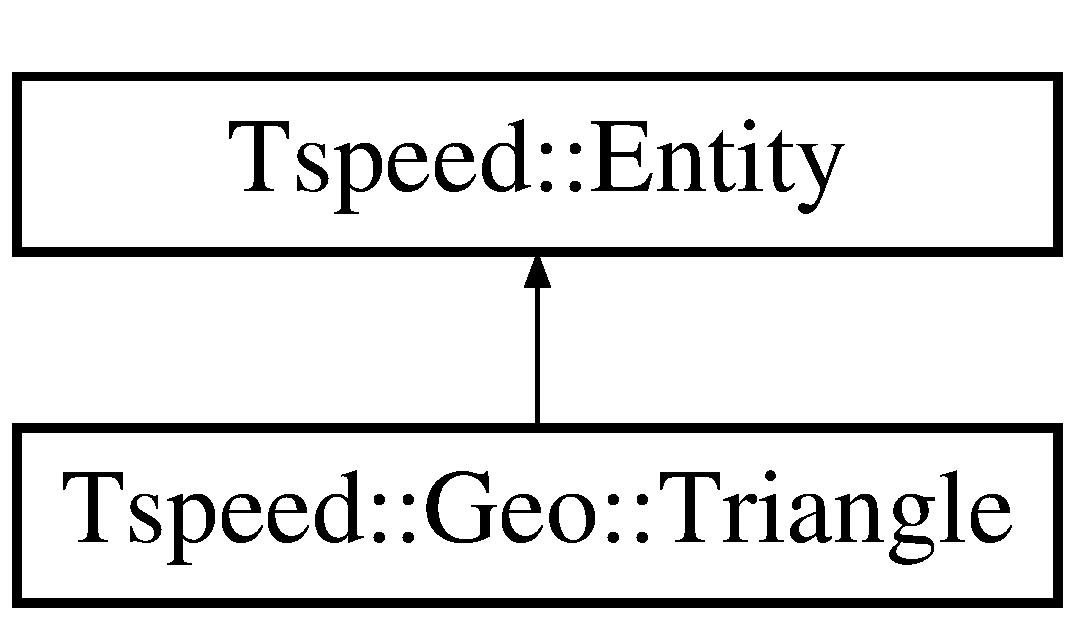
\includegraphics[height=2.000000cm]{classTspeed_1_1Geo_1_1Triangle}
\end{center}
\end{figure}
\subsection*{Public Member Functions}
\begin{DoxyCompactItemize}
\item 
\hyperlink{classTspeed_1_1Geo_1_1Triangle_a96ea06e6dbd9b707184c5e22d305e6e6}{Triangle} ()
\item 
\hyperlink{classTspeed_1_1Geo_1_1Triangle_a06a3c8a78d0e633b48df2a62db82e1cf}{Triangle} (const \hyperlink{classTspeed_1_1Geo_1_1Point}{Point} \&a, const \hyperlink{classTspeed_1_1Geo_1_1Point}{Point} \&b, const \hyperlink{classTspeed_1_1Geo_1_1Point}{Point} \&c)
\begin{DoxyCompactList}\small\item\em Create a triangle from three points. \end{DoxyCompactList}\item 
\hyperlink{classTspeed_1_1Geo_1_1Triangle_a3688a8a85846b3262366267d85e80d5a}{Triangle} (const \hyperlink{classTspeed_1_1Geo_1_1Triangle}{Triangle} \&)=default
\begin{DoxyCompactList}\small\item\em Copy constructor. \end{DoxyCompactList}\item 
\hyperlink{classTspeed_1_1Geo_1_1Triangle}{Triangle} \& \hyperlink{classTspeed_1_1Geo_1_1Triangle_a38b03bcff96b6ed334d381d56507c91d}{operator=} (const \hyperlink{classTspeed_1_1Geo_1_1Triangle}{Triangle} \&)
\begin{DoxyCompactList}\small\item\em Assignement. \end{DoxyCompactList}\item 
virtual \hyperlink{classTspeed_1_1Geo_1_1Triangle_af195c8c8c367a11fa9dc95f4a4ef8898}{$\sim$\-Triangle} ()
\item 
std\-::array$<$ \hyperlink{classTspeed_1_1Geo_1_1Point}{Point}, 3 $>$ \hyperlink{classTspeed_1_1Geo_1_1Triangle_a5749a0b4d9cec7c73fdfa13904ab04c6}{all\-\_\-pts} () const 
\begin{DoxyCompactList}\small\item\em Get all points of the triangle. \end{DoxyCompactList}\item 
std\-::array$<$ \hyperlink{classTspeed_1_1Geo_1_1Edge}{Edge}, 3 $>$ \hyperlink{classTspeed_1_1Geo_1_1Triangle_a95aad39ebd133e7fc23fd6a2431c601e}{all\-\_\-edges} () const 
\begin{DoxyCompactList}\small\item\em Get all edges of a triangle. \end{DoxyCompactList}\item 
\hyperlink{classTspeed_1_1Geo_1_1Point}{Point} const \& \hyperlink{classTspeed_1_1Geo_1_1Triangle_a6c4b1ba6d7adf584776089ecfc8d4f8e}{pt} (int i) const 
\begin{DoxyCompactList}\small\item\em Get a point. \end{DoxyCompactList}\item 
\hyperlink{classTspeed_1_1Geo_1_1Edge}{Edge} const \& \hyperlink{classTspeed_1_1Geo_1_1Triangle_aabfd53348c1c63905abf4eeda9cd42ae}{edg} (int i) const 
\begin{DoxyCompactList}\small\item\em Get a edge. \end{DoxyCompactList}\item 
Eigen\-::\-Matrix2d \hyperlink{classTspeed_1_1Geo_1_1Triangle_a936a5210cb5fdc598fa55a703b0d776d}{Jac} () const 
\begin{DoxyCompactList}\small\item\em Get Jacobian of the transformation from the reference triangle. \end{DoxyCompactList}\item 
Eigen\-::\-Matrix2d \hyperlink{classTspeed_1_1Geo_1_1Triangle_acadcc4f5328209374fa1060e42d564bb}{inv\-Jac} () const 
\begin{DoxyCompactList}\small\item\em Get the inverse Jacobian of the transformation from the reference triangle. \end{DoxyCompactList}\item 
double \hyperlink{classTspeed_1_1Geo_1_1Triangle_a2737a2218f6ecbf80e34e360fd2c0ccd}{det\-J} () const 
\begin{DoxyCompactList}\small\item\em Get the determinant of the Jacobian of the tranformation from the reference triangle. \end{DoxyCompactList}\item 
\hyperlink{classTspeed_1_1Geo_1_1Point}{Point} \hyperlink{classTspeed_1_1Geo_1_1Triangle_a3ae4d893a8a0b5612aa5530914fbe704}{map} (\hyperlink{classTspeed_1_1Geo_1_1Point}{Point} const \&p) const 
\begin{DoxyCompactList}\small\item\em Map a point from its relative position in the reference triangle to the physical point. \end{DoxyCompactList}\item 
\hyperlink{classTspeed_1_1Geo_1_1Point}{Point} \hyperlink{classTspeed_1_1Geo_1_1Triangle_aa607d5ba63bf021d0ca818c4727ff2c9}{invmap} (\hyperlink{classTspeed_1_1Geo_1_1Point}{Point} const \&p) const 
\begin{DoxyCompactList}\small\item\em Map a point from the physical triangle to the reference one. \end{DoxyCompactList}\item 
int const \& \hyperlink{classTspeed_1_1Geo_1_1Triangle_a9258f1265a916d2ed4ccf4c0d0ddcbb7}{neigh} (int i) const 
\begin{DoxyCompactList}\small\item\em Ged index of neighboring triangle on edge i. \end{DoxyCompactList}\item 
int const \& \hyperlink{classTspeed_1_1Geo_1_1Triangle_a223bb2cb8fc96ea689daa5e7312aa7ca}{neighedges} (int i) const 
\begin{DoxyCompactList}\small\item\em Index of the edge i in the nieghboring triangle. \end{DoxyCompactList}\item 
void \hyperlink{classTspeed_1_1Geo_1_1Triangle_a1d71aed7672a87aed76934626d671ba7}{set\-Neigh} (int i, int j)
\begin{DoxyCompactList}\small\item\em Set neighboring triangle. \end{DoxyCompactList}\item 
void \hyperlink{classTspeed_1_1Geo_1_1Triangle_a8c174fbb7b71ef4625f021166bd1c8a6}{set\-Neighedges} (int i, int j)
\begin{DoxyCompactList}\small\item\em Set index of the edge of the nieghboring triangle. \end{DoxyCompactList}\item 
void \hyperlink{classTspeed_1_1Geo_1_1Triangle_a91d1f81ecb8f0524257ea821245d6c3f}{print\-Neigh} () const 
\begin{DoxyCompactList}\small\item\em Pirnt neighbors for the current triangle. \end{DoxyCompactList}\item 
bool \hyperlink{classTspeed_1_1Geo_1_1Triangle_af35a8855e804d92c28a922aaa5abf187}{intriangle} (const \hyperlink{classTspeed_1_1Geo_1_1Point}{Point} \&p) const 
\begin{DoxyCompactList}\small\item\em Check if point p is in triangle. \end{DoxyCompactList}\end{DoxyCompactItemize}
\subsection*{Static Public Attributes}
\begin{DoxyCompactItemize}
\item 
static const int \hyperlink{classTspeed_1_1Geo_1_1Triangle_af01040fae660e384b7919ed166ed88ae}{num\-Vertices} =3
\end{DoxyCompactItemize}
\subsection*{Additional Inherited Members}


\subsection{Detailed Description}
Class describing a triangle. 

\subsection{Constructor \& Destructor Documentation}
\hypertarget{classTspeed_1_1Geo_1_1Triangle_a96ea06e6dbd9b707184c5e22d305e6e6}{\index{Tspeed\-::\-Geo\-::\-Triangle@{Tspeed\-::\-Geo\-::\-Triangle}!Triangle@{Triangle}}
\index{Triangle@{Triangle}!Tspeed::Geo::Triangle@{Tspeed\-::\-Geo\-::\-Triangle}}
\subsubsection[{Triangle}]{\setlength{\rightskip}{0pt plus 5cm}Tspeed\-::\-Geo\-::\-Triangle\-::\-Triangle (
\begin{DoxyParamCaption}
{}
\end{DoxyParamCaption}
)}}\label{classTspeed_1_1Geo_1_1Triangle_a96ea06e6dbd9b707184c5e22d305e6e6}
\hypertarget{classTspeed_1_1Geo_1_1Triangle_a06a3c8a78d0e633b48df2a62db82e1cf}{\index{Tspeed\-::\-Geo\-::\-Triangle@{Tspeed\-::\-Geo\-::\-Triangle}!Triangle@{Triangle}}
\index{Triangle@{Triangle}!Tspeed::Geo::Triangle@{Tspeed\-::\-Geo\-::\-Triangle}}
\subsubsection[{Triangle}]{\setlength{\rightskip}{0pt plus 5cm}Tspeed\-::\-Geo\-::\-Triangle\-::\-Triangle (
\begin{DoxyParamCaption}
\item[{const {\bf Point} \&}]{a, }
\item[{const {\bf Point} \&}]{b, }
\item[{const {\bf Point} \&}]{c}
\end{DoxyParamCaption}
)}}\label{classTspeed_1_1Geo_1_1Triangle_a06a3c8a78d0e633b48df2a62db82e1cf}


Create a triangle from three points. 


\begin{DoxyParams}{Parameters}
{\em a,b,c} & The three points \\
\hline
\end{DoxyParams}
\hypertarget{classTspeed_1_1Geo_1_1Triangle_a3688a8a85846b3262366267d85e80d5a}{\index{Tspeed\-::\-Geo\-::\-Triangle@{Tspeed\-::\-Geo\-::\-Triangle}!Triangle@{Triangle}}
\index{Triangle@{Triangle}!Tspeed::Geo::Triangle@{Tspeed\-::\-Geo\-::\-Triangle}}
\subsubsection[{Triangle}]{\setlength{\rightskip}{0pt plus 5cm}Tspeed\-::\-Geo\-::\-Triangle\-::\-Triangle (
\begin{DoxyParamCaption}
\item[{const {\bf Triangle} \&}]{}
\end{DoxyParamCaption}
)\hspace{0.3cm}{\ttfamily [default]}}}\label{classTspeed_1_1Geo_1_1Triangle_a3688a8a85846b3262366267d85e80d5a}


Copy constructor. 

\hypertarget{classTspeed_1_1Geo_1_1Triangle_af195c8c8c367a11fa9dc95f4a4ef8898}{\index{Tspeed\-::\-Geo\-::\-Triangle@{Tspeed\-::\-Geo\-::\-Triangle}!$\sim$\-Triangle@{$\sim$\-Triangle}}
\index{$\sim$\-Triangle@{$\sim$\-Triangle}!Tspeed::Geo::Triangle@{Tspeed\-::\-Geo\-::\-Triangle}}
\subsubsection[{$\sim$\-Triangle}]{\setlength{\rightskip}{0pt plus 5cm}virtual Tspeed\-::\-Geo\-::\-Triangle\-::$\sim$\-Triangle (
\begin{DoxyParamCaption}
{}
\end{DoxyParamCaption}
)\hspace{0.3cm}{\ttfamily [inline]}, {\ttfamily [virtual]}}}\label{classTspeed_1_1Geo_1_1Triangle_af195c8c8c367a11fa9dc95f4a4ef8898}


\subsection{Member Function Documentation}
\hypertarget{classTspeed_1_1Geo_1_1Triangle_a95aad39ebd133e7fc23fd6a2431c601e}{\index{Tspeed\-::\-Geo\-::\-Triangle@{Tspeed\-::\-Geo\-::\-Triangle}!all\-\_\-edges@{all\-\_\-edges}}
\index{all\-\_\-edges@{all\-\_\-edges}!Tspeed::Geo::Triangle@{Tspeed\-::\-Geo\-::\-Triangle}}
\subsubsection[{all\-\_\-edges}]{\setlength{\rightskip}{0pt plus 5cm}std\-::array$<${\bf Edge},3$>$ Tspeed\-::\-Geo\-::\-Triangle\-::all\-\_\-edges (
\begin{DoxyParamCaption}
{}
\end{DoxyParamCaption}
) const\hspace{0.3cm}{\ttfamily [inline]}}}\label{classTspeed_1_1Geo_1_1Triangle_a95aad39ebd133e7fc23fd6a2431c601e}


Get all edges of a triangle. 

\begin{DoxyReturn}{Returns}
An array of the three edge 
\end{DoxyReturn}
\hypertarget{classTspeed_1_1Geo_1_1Triangle_a5749a0b4d9cec7c73fdfa13904ab04c6}{\index{Tspeed\-::\-Geo\-::\-Triangle@{Tspeed\-::\-Geo\-::\-Triangle}!all\-\_\-pts@{all\-\_\-pts}}
\index{all\-\_\-pts@{all\-\_\-pts}!Tspeed::Geo::Triangle@{Tspeed\-::\-Geo\-::\-Triangle}}
\subsubsection[{all\-\_\-pts}]{\setlength{\rightskip}{0pt plus 5cm}std\-::array$<${\bf Point},3$>$ Tspeed\-::\-Geo\-::\-Triangle\-::all\-\_\-pts (
\begin{DoxyParamCaption}
{}
\end{DoxyParamCaption}
) const\hspace{0.3cm}{\ttfamily [inline]}}}\label{classTspeed_1_1Geo_1_1Triangle_a5749a0b4d9cec7c73fdfa13904ab04c6}


Get all points of the triangle. 

\begin{DoxyReturn}{Returns}
An array of three points 
\end{DoxyReturn}
\hypertarget{classTspeed_1_1Geo_1_1Triangle_a2737a2218f6ecbf80e34e360fd2c0ccd}{\index{Tspeed\-::\-Geo\-::\-Triangle@{Tspeed\-::\-Geo\-::\-Triangle}!det\-J@{det\-J}}
\index{det\-J@{det\-J}!Tspeed::Geo::Triangle@{Tspeed\-::\-Geo\-::\-Triangle}}
\subsubsection[{det\-J}]{\setlength{\rightskip}{0pt plus 5cm}double Tspeed\-::\-Geo\-::\-Triangle\-::det\-J (
\begin{DoxyParamCaption}
{}
\end{DoxyParamCaption}
) const}}\label{classTspeed_1_1Geo_1_1Triangle_a2737a2218f6ecbf80e34e360fd2c0ccd}


Get the determinant of the Jacobian of the tranformation from the reference triangle. 

\begin{DoxyReturn}{Returns}
the determinant of the Jacobian (i.\-e., Area(\-T)$\ast$2) 
\end{DoxyReturn}
\hypertarget{classTspeed_1_1Geo_1_1Triangle_aabfd53348c1c63905abf4eeda9cd42ae}{\index{Tspeed\-::\-Geo\-::\-Triangle@{Tspeed\-::\-Geo\-::\-Triangle}!edg@{edg}}
\index{edg@{edg}!Tspeed::Geo::Triangle@{Tspeed\-::\-Geo\-::\-Triangle}}
\subsubsection[{edg}]{\setlength{\rightskip}{0pt plus 5cm}{\bf Edge} const\& Tspeed\-::\-Geo\-::\-Triangle\-::edg (
\begin{DoxyParamCaption}
\item[{int}]{i}
\end{DoxyParamCaption}
) const\hspace{0.3cm}{\ttfamily [inline]}}}\label{classTspeed_1_1Geo_1_1Triangle_aabfd53348c1c63905abf4eeda9cd42ae}


Get a edge. 


\begin{DoxyParams}{Parameters}
{\em i} & Number of the edge in the triangle\\
\hline
\end{DoxyParams}
\begin{DoxyReturn}{Returns}
The i-\/th edge 
\end{DoxyReturn}
\hypertarget{classTspeed_1_1Geo_1_1Triangle_af35a8855e804d92c28a922aaa5abf187}{\index{Tspeed\-::\-Geo\-::\-Triangle@{Tspeed\-::\-Geo\-::\-Triangle}!intriangle@{intriangle}}
\index{intriangle@{intriangle}!Tspeed::Geo::Triangle@{Tspeed\-::\-Geo\-::\-Triangle}}
\subsubsection[{intriangle}]{\setlength{\rightskip}{0pt plus 5cm}bool Tspeed\-::\-Geo\-::\-Triangle\-::intriangle (
\begin{DoxyParamCaption}
\item[{const {\bf Point} \&}]{p}
\end{DoxyParamCaption}
) const}}\label{classTspeed_1_1Geo_1_1Triangle_af35a8855e804d92c28a922aaa5abf187}


Check if point p is in triangle. 


\begin{DoxyParams}{Parameters}
{\em p} & The point\\
\hline
\end{DoxyParams}
\begin{DoxyReturn}{Returns}
T\-R\-U\-E if the point is in the triangle 
\end{DoxyReturn}
\hypertarget{classTspeed_1_1Geo_1_1Triangle_acadcc4f5328209374fa1060e42d564bb}{\index{Tspeed\-::\-Geo\-::\-Triangle@{Tspeed\-::\-Geo\-::\-Triangle}!inv\-Jac@{inv\-Jac}}
\index{inv\-Jac@{inv\-Jac}!Tspeed::Geo::Triangle@{Tspeed\-::\-Geo\-::\-Triangle}}
\subsubsection[{inv\-Jac}]{\setlength{\rightskip}{0pt plus 5cm}Eigen\-::\-Matrix2d Tspeed\-::\-Geo\-::\-Triangle\-::inv\-Jac (
\begin{DoxyParamCaption}
{}
\end{DoxyParamCaption}
) const}}\label{classTspeed_1_1Geo_1_1Triangle_acadcc4f5328209374fa1060e42d564bb}


Get the inverse Jacobian of the transformation from the reference triangle. 

\begin{DoxyReturn}{Returns}
The inverse Jacobian, in matrix form 
\end{DoxyReturn}
\hypertarget{classTspeed_1_1Geo_1_1Triangle_aa607d5ba63bf021d0ca818c4727ff2c9}{\index{Tspeed\-::\-Geo\-::\-Triangle@{Tspeed\-::\-Geo\-::\-Triangle}!invmap@{invmap}}
\index{invmap@{invmap}!Tspeed::Geo::Triangle@{Tspeed\-::\-Geo\-::\-Triangle}}
\subsubsection[{invmap}]{\setlength{\rightskip}{0pt plus 5cm}{\bf Point} Tspeed\-::\-Geo\-::\-Triangle\-::invmap (
\begin{DoxyParamCaption}
\item[{{\bf Point} const \&}]{p}
\end{DoxyParamCaption}
) const}}\label{classTspeed_1_1Geo_1_1Triangle_aa607d5ba63bf021d0ca818c4727ff2c9}


Map a point from the physical triangle to the reference one. 


\begin{DoxyParams}{Parameters}
{\em p} & The physical point\\
\hline
\end{DoxyParams}
\begin{DoxyReturn}{Returns}
The point in the reference triangle 
\end{DoxyReturn}
\hypertarget{classTspeed_1_1Geo_1_1Triangle_a936a5210cb5fdc598fa55a703b0d776d}{\index{Tspeed\-::\-Geo\-::\-Triangle@{Tspeed\-::\-Geo\-::\-Triangle}!Jac@{Jac}}
\index{Jac@{Jac}!Tspeed::Geo::Triangle@{Tspeed\-::\-Geo\-::\-Triangle}}
\subsubsection[{Jac}]{\setlength{\rightskip}{0pt plus 5cm}Eigen\-::\-Matrix2d Tspeed\-::\-Geo\-::\-Triangle\-::\-Jac (
\begin{DoxyParamCaption}
{}
\end{DoxyParamCaption}
) const}}\label{classTspeed_1_1Geo_1_1Triangle_a936a5210cb5fdc598fa55a703b0d776d}


Get Jacobian of the transformation from the reference triangle. 

\begin{DoxyReturn}{Returns}
The Jacobian, in matrix form 
\end{DoxyReturn}
\hypertarget{classTspeed_1_1Geo_1_1Triangle_a3ae4d893a8a0b5612aa5530914fbe704}{\index{Tspeed\-::\-Geo\-::\-Triangle@{Tspeed\-::\-Geo\-::\-Triangle}!map@{map}}
\index{map@{map}!Tspeed::Geo::Triangle@{Tspeed\-::\-Geo\-::\-Triangle}}
\subsubsection[{map}]{\setlength{\rightskip}{0pt plus 5cm}{\bf Point} Tspeed\-::\-Geo\-::\-Triangle\-::map (
\begin{DoxyParamCaption}
\item[{{\bf Point} const \&}]{p}
\end{DoxyParamCaption}
) const}}\label{classTspeed_1_1Geo_1_1Triangle_a3ae4d893a8a0b5612aa5530914fbe704}


Map a point from its relative position in the reference triangle to the physical point. 


\begin{DoxyParams}{Parameters}
{\em p} & The point in the reference triangle\\
\hline
\end{DoxyParams}
\begin{DoxyReturn}{Returns}
The physical point in the actual triangle 
\end{DoxyReturn}
\hypertarget{classTspeed_1_1Geo_1_1Triangle_a9258f1265a916d2ed4ccf4c0d0ddcbb7}{\index{Tspeed\-::\-Geo\-::\-Triangle@{Tspeed\-::\-Geo\-::\-Triangle}!neigh@{neigh}}
\index{neigh@{neigh}!Tspeed::Geo::Triangle@{Tspeed\-::\-Geo\-::\-Triangle}}
\subsubsection[{neigh}]{\setlength{\rightskip}{0pt plus 5cm}int const\& Tspeed\-::\-Geo\-::\-Triangle\-::neigh (
\begin{DoxyParamCaption}
\item[{int}]{i}
\end{DoxyParamCaption}
) const\hspace{0.3cm}{\ttfamily [inline]}}}\label{classTspeed_1_1Geo_1_1Triangle_a9258f1265a916d2ed4ccf4c0d0ddcbb7}


Ged index of neighboring triangle on edge i. 


\begin{DoxyParams}{Parameters}
{\em i} & \hyperlink{classTspeed_1_1Geo_1_1Edge}{Edge} of the triangle\\
\hline
\end{DoxyParams}
\begin{DoxyReturn}{Returns}
Index of the neighbor 
\end{DoxyReturn}
\hypertarget{classTspeed_1_1Geo_1_1Triangle_a223bb2cb8fc96ea689daa5e7312aa7ca}{\index{Tspeed\-::\-Geo\-::\-Triangle@{Tspeed\-::\-Geo\-::\-Triangle}!neighedges@{neighedges}}
\index{neighedges@{neighedges}!Tspeed::Geo::Triangle@{Tspeed\-::\-Geo\-::\-Triangle}}
\subsubsection[{neighedges}]{\setlength{\rightskip}{0pt plus 5cm}int const\& Tspeed\-::\-Geo\-::\-Triangle\-::neighedges (
\begin{DoxyParamCaption}
\item[{int}]{i}
\end{DoxyParamCaption}
) const\hspace{0.3cm}{\ttfamily [inline]}}}\label{classTspeed_1_1Geo_1_1Triangle_a223bb2cb8fc96ea689daa5e7312aa7ca}


Index of the edge i in the nieghboring triangle. 


\begin{DoxyParams}{Parameters}
{\em i} & \hyperlink{classTspeed_1_1Geo_1_1Edge}{Edge} of the present triangle\\
\hline
\end{DoxyParams}
\begin{DoxyReturn}{Returns}
Index of the edge in the neighboring triangle 
\end{DoxyReturn}
\hypertarget{classTspeed_1_1Geo_1_1Triangle_a38b03bcff96b6ed334d381d56507c91d}{\index{Tspeed\-::\-Geo\-::\-Triangle@{Tspeed\-::\-Geo\-::\-Triangle}!operator=@{operator=}}
\index{operator=@{operator=}!Tspeed::Geo::Triangle@{Tspeed\-::\-Geo\-::\-Triangle}}
\subsubsection[{operator=}]{\setlength{\rightskip}{0pt plus 5cm}{\bf Triangle} \& Tspeed\-::\-Geo\-::\-Triangle\-::operator= (
\begin{DoxyParamCaption}
\item[{const {\bf Triangle} \&}]{t}
\end{DoxyParamCaption}
)}}\label{classTspeed_1_1Geo_1_1Triangle_a38b03bcff96b6ed334d381d56507c91d}


Assignement. 

\hypertarget{classTspeed_1_1Geo_1_1Triangle_a91d1f81ecb8f0524257ea821245d6c3f}{\index{Tspeed\-::\-Geo\-::\-Triangle@{Tspeed\-::\-Geo\-::\-Triangle}!print\-Neigh@{print\-Neigh}}
\index{print\-Neigh@{print\-Neigh}!Tspeed::Geo::Triangle@{Tspeed\-::\-Geo\-::\-Triangle}}
\subsubsection[{print\-Neigh}]{\setlength{\rightskip}{0pt plus 5cm}void Tspeed\-::\-Geo\-::\-Triangle\-::print\-Neigh (
\begin{DoxyParamCaption}
{}
\end{DoxyParamCaption}
) const\hspace{0.3cm}{\ttfamily [inline]}}}\label{classTspeed_1_1Geo_1_1Triangle_a91d1f81ecb8f0524257ea821245d6c3f}


Pirnt neighbors for the current triangle. 

\hypertarget{classTspeed_1_1Geo_1_1Triangle_a6c4b1ba6d7adf584776089ecfc8d4f8e}{\index{Tspeed\-::\-Geo\-::\-Triangle@{Tspeed\-::\-Geo\-::\-Triangle}!pt@{pt}}
\index{pt@{pt}!Tspeed::Geo::Triangle@{Tspeed\-::\-Geo\-::\-Triangle}}
\subsubsection[{pt}]{\setlength{\rightskip}{0pt plus 5cm}{\bf Point} const\& Tspeed\-::\-Geo\-::\-Triangle\-::pt (
\begin{DoxyParamCaption}
\item[{int}]{i}
\end{DoxyParamCaption}
) const\hspace{0.3cm}{\ttfamily [inline]}}}\label{classTspeed_1_1Geo_1_1Triangle_a6c4b1ba6d7adf584776089ecfc8d4f8e}


Get a point. 


\begin{DoxyParams}{Parameters}
{\em i} & Number of the point in the triangle\\
\hline
\end{DoxyParams}
\begin{DoxyReturn}{Returns}
The i-\/th point 
\end{DoxyReturn}
\hypertarget{classTspeed_1_1Geo_1_1Triangle_a1d71aed7672a87aed76934626d671ba7}{\index{Tspeed\-::\-Geo\-::\-Triangle@{Tspeed\-::\-Geo\-::\-Triangle}!set\-Neigh@{set\-Neigh}}
\index{set\-Neigh@{set\-Neigh}!Tspeed::Geo::Triangle@{Tspeed\-::\-Geo\-::\-Triangle}}
\subsubsection[{set\-Neigh}]{\setlength{\rightskip}{0pt plus 5cm}void Tspeed\-::\-Geo\-::\-Triangle\-::set\-Neigh (
\begin{DoxyParamCaption}
\item[{int}]{i, }
\item[{int}]{j}
\end{DoxyParamCaption}
)\hspace{0.3cm}{\ttfamily [inline]}}}\label{classTspeed_1_1Geo_1_1Triangle_a1d71aed7672a87aed76934626d671ba7}


Set neighboring triangle. 


\begin{DoxyParams}{Parameters}
{\em i} & \hyperlink{classTspeed_1_1Geo_1_1Edge}{Edge} of the current triangle \\
\hline
{\em j} & Index of the neighbor \\
\hline
\end{DoxyParams}
\hypertarget{classTspeed_1_1Geo_1_1Triangle_a8c174fbb7b71ef4625f021166bd1c8a6}{\index{Tspeed\-::\-Geo\-::\-Triangle@{Tspeed\-::\-Geo\-::\-Triangle}!set\-Neighedges@{set\-Neighedges}}
\index{set\-Neighedges@{set\-Neighedges}!Tspeed::Geo::Triangle@{Tspeed\-::\-Geo\-::\-Triangle}}
\subsubsection[{set\-Neighedges}]{\setlength{\rightskip}{0pt plus 5cm}void Tspeed\-::\-Geo\-::\-Triangle\-::set\-Neighedges (
\begin{DoxyParamCaption}
\item[{int}]{i, }
\item[{int}]{j}
\end{DoxyParamCaption}
)\hspace{0.3cm}{\ttfamily [inline]}}}\label{classTspeed_1_1Geo_1_1Triangle_a8c174fbb7b71ef4625f021166bd1c8a6}


Set index of the edge of the nieghboring triangle. 


\begin{DoxyParams}{Parameters}
{\em i} & \hyperlink{classTspeed_1_1Geo_1_1Edge}{Edge} of the current trinagle \\
\hline
{\em j} & \hyperlink{classTspeed_1_1Geo_1_1Edge}{Edge} in the neighboring triangle \\
\hline
\end{DoxyParams}


\subsection{Member Data Documentation}
\hypertarget{classTspeed_1_1Geo_1_1Triangle_af01040fae660e384b7919ed166ed88ae}{\index{Tspeed\-::\-Geo\-::\-Triangle@{Tspeed\-::\-Geo\-::\-Triangle}!num\-Vertices@{num\-Vertices}}
\index{num\-Vertices@{num\-Vertices}!Tspeed::Geo::Triangle@{Tspeed\-::\-Geo\-::\-Triangle}}
\subsubsection[{num\-Vertices}]{\setlength{\rightskip}{0pt plus 5cm}const int Tspeed\-::\-Geo\-::\-Triangle\-::num\-Vertices =3\hspace{0.3cm}{\ttfamily [static]}}}\label{classTspeed_1_1Geo_1_1Triangle_af01040fae660e384b7919ed166ed88ae}


The documentation for this class was generated from the following files\-:\begin{DoxyCompactItemize}
\item 
lib/include/\hyperlink{Geometry_8hpp}{Geometry.\-hpp}\item 
lib/src/\hyperlink{Geometry_8cpp}{Geometry.\-cpp}\end{DoxyCompactItemize}

\chapter{File Documentation}
\hypertarget{Lamb_8cpp}{\section{Examples/src/\-Lamb.cpp File Reference}
\label{Lamb_8cpp}\index{Examples/src/\-Lamb.\-cpp@{Examples/src/\-Lamb.\-cpp}}
}
{\ttfamily \#include \char`\"{}T\-S\-P\-E\-E\-D.\-hpp\char`\"{}}\\*
{\ttfamily \#include $<$iostream$>$}\\*
\subsection*{Functions}
\begin{DoxyCompactItemize}
\item 
int \hyperlink{Lamb_8cpp_ae66f6b31b5ad750f1fe042a706a4e3d4}{main} ()
\end{DoxyCompactItemize}


\subsection{Function Documentation}
\hypertarget{Lamb_8cpp_ae66f6b31b5ad750f1fe042a706a4e3d4}{\index{Lamb.\-cpp@{Lamb.\-cpp}!main@{main}}
\index{main@{main}!Lamb.cpp@{Lamb.\-cpp}}
\subsubsection[{main}]{\setlength{\rightskip}{0pt plus 5cm}int main (
\begin{DoxyParamCaption}
{}
\end{DoxyParamCaption}
)}}\label{Lamb_8cpp_ae66f6b31b5ad750f1fe042a706a4e3d4}

\hypertarget{wedge_8cpp}{\section{Examples/src/wedge.cpp File Reference}
\label{wedge_8cpp}\index{Examples/src/wedge.\-cpp@{Examples/src/wedge.\-cpp}}
}
{\ttfamily \#include \char`\"{}T\-S\-P\-E\-E\-D.\-hpp\char`\"{}}\\*
{\ttfamily \#include $<$iostream$>$}\\*
{\ttfamily \#include $<$memory$>$}\\*
\subsection*{Functions}
\begin{DoxyCompactItemize}
\item 
void \hyperlink{wedge_8cpp_ad50ebb1944e24e11e66dabede90c026b}{wedge\-\_\-init\-\_\-param} (double l, double m, double rho, double cf, double csurf, double \&k, double \&q, double \&s, double \&beta)
\item 
int \hyperlink{wedge_8cpp_ae66f6b31b5ad750f1fe042a706a4e3d4}{main} ()
\end{DoxyCompactItemize}


\subsection{Function Documentation}
\hypertarget{wedge_8cpp_ae66f6b31b5ad750f1fe042a706a4e3d4}{\index{wedge.\-cpp@{wedge.\-cpp}!main@{main}}
\index{main@{main}!wedge.cpp@{wedge.\-cpp}}
\subsubsection[{main}]{\setlength{\rightskip}{0pt plus 5cm}int main (
\begin{DoxyParamCaption}
{}
\end{DoxyParamCaption}
)}}\label{wedge_8cpp_ae66f6b31b5ad750f1fe042a706a4e3d4}
\hypertarget{wedge_8cpp_ad50ebb1944e24e11e66dabede90c026b}{\index{wedge.\-cpp@{wedge.\-cpp}!wedge\-\_\-init\-\_\-param@{wedge\-\_\-init\-\_\-param}}
\index{wedge\-\_\-init\-\_\-param@{wedge\-\_\-init\-\_\-param}!wedge.cpp@{wedge.\-cpp}}
\subsubsection[{wedge\-\_\-init\-\_\-param}]{\setlength{\rightskip}{0pt plus 5cm}void wedge\-\_\-init\-\_\-param (
\begin{DoxyParamCaption}
\item[{double}]{l, }
\item[{double}]{m, }
\item[{double}]{rho, }
\item[{double}]{cf, }
\item[{double}]{csurf, }
\item[{double \&}]{k, }
\item[{double \&}]{q, }
\item[{double \&}]{s, }
\item[{double \&}]{beta}
\end{DoxyParamCaption}
)}}\label{wedge_8cpp_ad50ebb1944e24e11e66dabede90c026b}

\hypertarget{Dunavant_8hpp}{\section{lib/include/\-Dunavant.hpp File Reference}
\label{Dunavant_8hpp}\index{lib/include/\-Dunavant.\-hpp@{lib/include/\-Dunavant.\-hpp}}
}


Header files for the implementation of the Dunavant rules.  


\subsection*{Functions}
\begin{DoxyCompactItemize}
\item 
int \hyperlink{Dunavant_8hpp_a49f9323b787a4399cf9affa237f7f6d2}{dunavant\-\_\-degree} (int rule)
\item 
int \hyperlink{Dunavant_8hpp_a1506127b60e81139ccd544a035465548}{dunavant\-\_\-order\-\_\-num} (int rule)
\item 
void \hyperlink{Dunavant_8hpp_a3b388ae21eee20f71f7bca9d357e26d5}{dunavant\-\_\-rule} (int rule, int order\-\_\-num, double xy\mbox{[}$\,$\mbox{]}, double w\mbox{[}$\,$\mbox{]})
\item 
int \hyperlink{Dunavant_8hpp_af6a4b0c6021f8d06ca8c1740967141a1}{dunavant\-\_\-rule\-\_\-num} (void)
\item 
int $\ast$ \hyperlink{Dunavant_8hpp_a5ae0dfda7f95af1106f0098a13cd9dc6}{dunavant\-\_\-suborder} (int rule, int suborder\-\_\-num)
\item 
int \hyperlink{Dunavant_8hpp_a1326280b05bdc27a67d069b612f3fbed}{dunavant\-\_\-suborder\-\_\-num} (int rule)
\item 
void \hyperlink{Dunavant_8hpp_aa87fd1deaae77a9a880af5c2ef847c9f}{dunavant\-\_\-subrule} (int rule, int suborder\-\_\-num, double suborder\-\_\-xyz\mbox{[}$\,$\mbox{]}, double suborder\-\_\-w\mbox{[}$\,$\mbox{]})
\item 
void \hyperlink{Dunavant_8hpp_ad49d9c036c90b72897590198df6269ce}{dunavant\-\_\-subrule\-\_\-01} (int suborder\-\_\-num, double suborder\-\_\-xyz\mbox{[}$\,$\mbox{]}, double suborder\-\_\-w\mbox{[}$\,$\mbox{]})
\item 
void \hyperlink{Dunavant_8hpp_a2ca3fa64053f25831f1cd5b3a4a5f58c}{dunavant\-\_\-subrule\-\_\-02} (int suborder\-\_\-num, double suborder\-\_\-xyz\mbox{[}$\,$\mbox{]}, double suborder\-\_\-w\mbox{[}$\,$\mbox{]})
\item 
void \hyperlink{Dunavant_8hpp_a2b2e89d9440289b57250244eff25867b}{dunavant\-\_\-subrule\-\_\-03} (int suborder\-\_\-num, double suborder\-\_\-xyz\mbox{[}$\,$\mbox{]}, double suborder\-\_\-w\mbox{[}$\,$\mbox{]})
\item 
void \hyperlink{Dunavant_8hpp_ae5ed81003214e3c0f0e8c37f949169fe}{dunavant\-\_\-subrule\-\_\-04} (int suborder\-\_\-num, double suborder\-\_\-xyz\mbox{[}$\,$\mbox{]}, double suborder\-\_\-w\mbox{[}$\,$\mbox{]})
\item 
void \hyperlink{Dunavant_8hpp_aba7e9583001bbc0cae3be5499ef04d72}{dunavant\-\_\-subrule\-\_\-05} (int suborder\-\_\-num, double suborder\-\_\-xyz\mbox{[}$\,$\mbox{]}, double suborder\-\_\-w\mbox{[}$\,$\mbox{]})
\item 
void \hyperlink{Dunavant_8hpp_a02482c6daea6b0bc58d9517f5c16c379}{dunavant\-\_\-subrule\-\_\-06} (int suborder\-\_\-num, double suborder\-\_\-xyz\mbox{[}$\,$\mbox{]}, double suborder\-\_\-w\mbox{[}$\,$\mbox{]})
\item 
void \hyperlink{Dunavant_8hpp_aea59d99379c245680548521b211eaeca}{dunavant\-\_\-subrule\-\_\-07} (int suborder\-\_\-num, double suborder\-\_\-xyz\mbox{[}$\,$\mbox{]}, double suborder\-\_\-w\mbox{[}$\,$\mbox{]})
\item 
void \hyperlink{Dunavant_8hpp_ad4f38a8cba4481fa7a1fa27b1016904d}{dunavant\-\_\-subrule\-\_\-08} (int suborder\-\_\-num, double suborder\-\_\-xyz\mbox{[}$\,$\mbox{]}, double suborder\-\_\-w\mbox{[}$\,$\mbox{]})
\item 
void \hyperlink{Dunavant_8hpp_a0ddc38f4d91417dfcda46a9ce326ef27}{dunavant\-\_\-subrule\-\_\-09} (int suborder\-\_\-num, double suborder\-\_\-xyz\mbox{[}$\,$\mbox{]}, double suborder\-\_\-w\mbox{[}$\,$\mbox{]})
\item 
void \hyperlink{Dunavant_8hpp_a7741f9fae510fd8931f2d1548b6fc35f}{dunavant\-\_\-subrule\-\_\-10} (int suborder\-\_\-num, double suborder\-\_\-xyz\mbox{[}$\,$\mbox{]}, double suborder\-\_\-w\mbox{[}$\,$\mbox{]})
\item 
void \hyperlink{Dunavant_8hpp_a24cdd61e8c13df25b28156c3968104b9}{dunavant\-\_\-subrule\-\_\-11} (int suborder\-\_\-num, double suborder\-\_\-xyz\mbox{[}$\,$\mbox{]}, double suborder\-\_\-w\mbox{[}$\,$\mbox{]})
\item 
void \hyperlink{Dunavant_8hpp_ae1fdef943fae2a5b8c25fafd3b532d04}{dunavant\-\_\-subrule\-\_\-12} (int suborder\-\_\-num, double suborder\-\_\-xyz\mbox{[}$\,$\mbox{]}, double suborder\-\_\-w\mbox{[}$\,$\mbox{]})
\item 
void \hyperlink{Dunavant_8hpp_ad474bd0c4bd21ba12ce2727b438c860c}{dunavant\-\_\-subrule\-\_\-13} (int suborder\-\_\-num, double suborder\-\_\-xyz\mbox{[}$\,$\mbox{]}, double suborder\-\_\-w\mbox{[}$\,$\mbox{]})
\item 
void \hyperlink{Dunavant_8hpp_aee910186e94d9f2c8053b2b2111c280b}{dunavant\-\_\-subrule\-\_\-14} (int suborder\-\_\-num, double suborder\-\_\-xyz\mbox{[}$\,$\mbox{]}, double suborder\-\_\-w\mbox{[}$\,$\mbox{]})
\item 
void \hyperlink{Dunavant_8hpp_ad9f03b78d7a3ee1f9aed7b146ed595c3}{dunavant\-\_\-subrule\-\_\-15} (int suborder\-\_\-num, double suborder\-\_\-xyz\mbox{[}$\,$\mbox{]}, double suborder\-\_\-w\mbox{[}$\,$\mbox{]})
\item 
void \hyperlink{Dunavant_8hpp_afddf4a586050bddf92337ff6b2a8eaf8}{dunavant\-\_\-subrule\-\_\-16} (int suborder\-\_\-num, double suborder\-\_\-xyz\mbox{[}$\,$\mbox{]}, double suborder\-\_\-w\mbox{[}$\,$\mbox{]})
\item 
void \hyperlink{Dunavant_8hpp_a23dc449a4827d81963820b24c9981d63}{dunavant\-\_\-subrule\-\_\-17} (int suborder\-\_\-num, double suborder\-\_\-xyz\mbox{[}$\,$\mbox{]}, double suborder\-\_\-w\mbox{[}$\,$\mbox{]})
\item 
void \hyperlink{Dunavant_8hpp_a532b8781542b64fcb43f390cdb3519dc}{dunavant\-\_\-subrule\-\_\-18} (int suborder\-\_\-num, double suborder\-\_\-xyz\mbox{[}$\,$\mbox{]}, double suborder\-\_\-w\mbox{[}$\,$\mbox{]})
\item 
void \hyperlink{Dunavant_8hpp_aea55210744d05c62f7bc40c0cc67bbaf}{dunavant\-\_\-subrule\-\_\-19} (int suborder\-\_\-num, double suborder\-\_\-xyz\mbox{[}$\,$\mbox{]}, double suborder\-\_\-w\mbox{[}$\,$\mbox{]})
\item 
void \hyperlink{Dunavant_8hpp_a30bd0d0c727fc24773cf2629dd18be72}{dunavant\-\_\-subrule\-\_\-20} (int suborder\-\_\-num, double suborder\-\_\-xyz\mbox{[}$\,$\mbox{]}, double suborder\-\_\-w\mbox{[}$\,$\mbox{]})
\item 
void \hyperlink{Dunavant_8hpp_a0f78f0152c268c49404ccc0c2d8d9d83}{file\-\_\-name\-\_\-inc} (char $\ast$file\-\_\-name)
\item 
int \hyperlink{Dunavant_8hpp_a36f800e4593bdd258feaeb43cf42adf7}{i4\-\_\-max} (int i1, int i2)
\item 
int \hyperlink{Dunavant_8hpp_ae73c30e1658d722ce9ff2e671db331ca}{i4\-\_\-min} (int i1, int i2)
\item 
int \hyperlink{Dunavant_8hpp_a0977ecce2ec88e382435b4bbc08bbdf7}{i4\-\_\-modp} (int i, int j)
\item 
int \hyperlink{Dunavant_8hpp_adf604b639ecc974176142f7265829259}{i4\-\_\-wrap} (int ival, int ilo, int ihi)
\item 
double \hyperlink{Dunavant_8hpp_ae59e4d9f04c3be0347cc77d9f0a5b221}{r8\-\_\-huge} (void)
\item 
int \hyperlink{Dunavant_8hpp_a7e0d15a4d0accb8c91928f44aa302394}{r8\-\_\-nint} (double x)
\item 
void \hyperlink{Dunavant_8hpp_a25a044f86e2618a1db0da8a925f2572d}{reference\-\_\-to\-\_\-physical\-\_\-t3} (double t\mbox{[}$\,$\mbox{]}, int n, double ref\mbox{[}$\,$\mbox{]}, double phy\mbox{[}$\,$\mbox{]})
\item 
int \hyperlink{Dunavant_8hpp_aaaab7eaef7b83f16504a609979ac5c7e}{s\-\_\-len\-\_\-trim} (char $\ast$s)
\item 
void \hyperlink{Dunavant_8hpp_a02d8f81e512334c1e2e5be025c41afa8}{timestamp} (void)
\item 
char $\ast$ \hyperlink{Dunavant_8hpp_a887a2ef0f2104b41fc76c017d6b6bf78}{timestring} (void)
\item 
double \hyperlink{Dunavant_8hpp_a08a0e9db99fb867596e84d1871713606}{triangle\-\_\-area} (double t\mbox{[}2 $\ast$3\mbox{]})
\item 
void \hyperlink{Dunavant_8hpp_af9c39491facec8d0f07a1a458c4323e8}{triangle\-\_\-points\-\_\-plot} (char $\ast$file\-\_\-name, double node\-\_\-xy\mbox{[}$\,$\mbox{]}, int node\-\_\-show, int point\-\_\-num, double point\-\_\-xy\mbox{[}$\,$\mbox{]}, int point\-\_\-show)
\end{DoxyCompactItemize}


\subsection{Detailed Description}
Header files for the implementation of the Dunavant rules. \begin{DoxyAuthor}{Author}
John Burkardt 
\end{DoxyAuthor}


\subsection{Function Documentation}
\hypertarget{Dunavant_8hpp_a49f9323b787a4399cf9affa237f7f6d2}{\index{Dunavant.\-hpp@{Dunavant.\-hpp}!dunavant\-\_\-degree@{dunavant\-\_\-degree}}
\index{dunavant\-\_\-degree@{dunavant\-\_\-degree}!Dunavant.hpp@{Dunavant.\-hpp}}
\subsubsection[{dunavant\-\_\-degree}]{\setlength{\rightskip}{0pt plus 5cm}int dunavant\-\_\-degree (
\begin{DoxyParamCaption}
\item[{int}]{rule}
\end{DoxyParamCaption}
)}}\label{Dunavant_8hpp_a49f9323b787a4399cf9affa237f7f6d2}
\hypertarget{Dunavant_8hpp_a1506127b60e81139ccd544a035465548}{\index{Dunavant.\-hpp@{Dunavant.\-hpp}!dunavant\-\_\-order\-\_\-num@{dunavant\-\_\-order\-\_\-num}}
\index{dunavant\-\_\-order\-\_\-num@{dunavant\-\_\-order\-\_\-num}!Dunavant.hpp@{Dunavant.\-hpp}}
\subsubsection[{dunavant\-\_\-order\-\_\-num}]{\setlength{\rightskip}{0pt plus 5cm}int dunavant\-\_\-order\-\_\-num (
\begin{DoxyParamCaption}
\item[{int}]{rule}
\end{DoxyParamCaption}
)}}\label{Dunavant_8hpp_a1506127b60e81139ccd544a035465548}
\hypertarget{Dunavant_8hpp_a3b388ae21eee20f71f7bca9d357e26d5}{\index{Dunavant.\-hpp@{Dunavant.\-hpp}!dunavant\-\_\-rule@{dunavant\-\_\-rule}}
\index{dunavant\-\_\-rule@{dunavant\-\_\-rule}!Dunavant.hpp@{Dunavant.\-hpp}}
\subsubsection[{dunavant\-\_\-rule}]{\setlength{\rightskip}{0pt plus 5cm}void dunavant\-\_\-rule (
\begin{DoxyParamCaption}
\item[{int}]{rule, }
\item[{int}]{order\-\_\-num, }
\item[{double}]{xy\mbox{[}$\,$\mbox{]}, }
\item[{double}]{w\mbox{[}$\,$\mbox{]}}
\end{DoxyParamCaption}
)}}\label{Dunavant_8hpp_a3b388ae21eee20f71f7bca9d357e26d5}
\hypertarget{Dunavant_8hpp_af6a4b0c6021f8d06ca8c1740967141a1}{\index{Dunavant.\-hpp@{Dunavant.\-hpp}!dunavant\-\_\-rule\-\_\-num@{dunavant\-\_\-rule\-\_\-num}}
\index{dunavant\-\_\-rule\-\_\-num@{dunavant\-\_\-rule\-\_\-num}!Dunavant.hpp@{Dunavant.\-hpp}}
\subsubsection[{dunavant\-\_\-rule\-\_\-num}]{\setlength{\rightskip}{0pt plus 5cm}int dunavant\-\_\-rule\-\_\-num (
\begin{DoxyParamCaption}
\item[{void}]{}
\end{DoxyParamCaption}
)}}\label{Dunavant_8hpp_af6a4b0c6021f8d06ca8c1740967141a1}
\hypertarget{Dunavant_8hpp_a5ae0dfda7f95af1106f0098a13cd9dc6}{\index{Dunavant.\-hpp@{Dunavant.\-hpp}!dunavant\-\_\-suborder@{dunavant\-\_\-suborder}}
\index{dunavant\-\_\-suborder@{dunavant\-\_\-suborder}!Dunavant.hpp@{Dunavant.\-hpp}}
\subsubsection[{dunavant\-\_\-suborder}]{\setlength{\rightskip}{0pt plus 5cm}int$\ast$ dunavant\-\_\-suborder (
\begin{DoxyParamCaption}
\item[{int}]{rule, }
\item[{int}]{suborder\-\_\-num}
\end{DoxyParamCaption}
)}}\label{Dunavant_8hpp_a5ae0dfda7f95af1106f0098a13cd9dc6}
\hypertarget{Dunavant_8hpp_a1326280b05bdc27a67d069b612f3fbed}{\index{Dunavant.\-hpp@{Dunavant.\-hpp}!dunavant\-\_\-suborder\-\_\-num@{dunavant\-\_\-suborder\-\_\-num}}
\index{dunavant\-\_\-suborder\-\_\-num@{dunavant\-\_\-suborder\-\_\-num}!Dunavant.hpp@{Dunavant.\-hpp}}
\subsubsection[{dunavant\-\_\-suborder\-\_\-num}]{\setlength{\rightskip}{0pt plus 5cm}int dunavant\-\_\-suborder\-\_\-num (
\begin{DoxyParamCaption}
\item[{int}]{rule}
\end{DoxyParamCaption}
)}}\label{Dunavant_8hpp_a1326280b05bdc27a67d069b612f3fbed}
\hypertarget{Dunavant_8hpp_aa87fd1deaae77a9a880af5c2ef847c9f}{\index{Dunavant.\-hpp@{Dunavant.\-hpp}!dunavant\-\_\-subrule@{dunavant\-\_\-subrule}}
\index{dunavant\-\_\-subrule@{dunavant\-\_\-subrule}!Dunavant.hpp@{Dunavant.\-hpp}}
\subsubsection[{dunavant\-\_\-subrule}]{\setlength{\rightskip}{0pt plus 5cm}void dunavant\-\_\-subrule (
\begin{DoxyParamCaption}
\item[{int}]{rule, }
\item[{int}]{suborder\-\_\-num, }
\item[{double}]{suborder\-\_\-xyz\mbox{[}$\,$\mbox{]}, }
\item[{double}]{suborder\-\_\-w\mbox{[}$\,$\mbox{]}}
\end{DoxyParamCaption}
)}}\label{Dunavant_8hpp_aa87fd1deaae77a9a880af5c2ef847c9f}
\hypertarget{Dunavant_8hpp_ad49d9c036c90b72897590198df6269ce}{\index{Dunavant.\-hpp@{Dunavant.\-hpp}!dunavant\-\_\-subrule\-\_\-01@{dunavant\-\_\-subrule\-\_\-01}}
\index{dunavant\-\_\-subrule\-\_\-01@{dunavant\-\_\-subrule\-\_\-01}!Dunavant.hpp@{Dunavant.\-hpp}}
\subsubsection[{dunavant\-\_\-subrule\-\_\-01}]{\setlength{\rightskip}{0pt plus 5cm}void dunavant\-\_\-subrule\-\_\-01 (
\begin{DoxyParamCaption}
\item[{int}]{suborder\-\_\-num, }
\item[{double}]{suborder\-\_\-xyz\mbox{[}$\,$\mbox{]}, }
\item[{double}]{suborder\-\_\-w\mbox{[}$\,$\mbox{]}}
\end{DoxyParamCaption}
)}}\label{Dunavant_8hpp_ad49d9c036c90b72897590198df6269ce}
\hypertarget{Dunavant_8hpp_a2ca3fa64053f25831f1cd5b3a4a5f58c}{\index{Dunavant.\-hpp@{Dunavant.\-hpp}!dunavant\-\_\-subrule\-\_\-02@{dunavant\-\_\-subrule\-\_\-02}}
\index{dunavant\-\_\-subrule\-\_\-02@{dunavant\-\_\-subrule\-\_\-02}!Dunavant.hpp@{Dunavant.\-hpp}}
\subsubsection[{dunavant\-\_\-subrule\-\_\-02}]{\setlength{\rightskip}{0pt plus 5cm}void dunavant\-\_\-subrule\-\_\-02 (
\begin{DoxyParamCaption}
\item[{int}]{suborder\-\_\-num, }
\item[{double}]{suborder\-\_\-xyz\mbox{[}$\,$\mbox{]}, }
\item[{double}]{suborder\-\_\-w\mbox{[}$\,$\mbox{]}}
\end{DoxyParamCaption}
)}}\label{Dunavant_8hpp_a2ca3fa64053f25831f1cd5b3a4a5f58c}
\hypertarget{Dunavant_8hpp_a2b2e89d9440289b57250244eff25867b}{\index{Dunavant.\-hpp@{Dunavant.\-hpp}!dunavant\-\_\-subrule\-\_\-03@{dunavant\-\_\-subrule\-\_\-03}}
\index{dunavant\-\_\-subrule\-\_\-03@{dunavant\-\_\-subrule\-\_\-03}!Dunavant.hpp@{Dunavant.\-hpp}}
\subsubsection[{dunavant\-\_\-subrule\-\_\-03}]{\setlength{\rightskip}{0pt plus 5cm}void dunavant\-\_\-subrule\-\_\-03 (
\begin{DoxyParamCaption}
\item[{int}]{suborder\-\_\-num, }
\item[{double}]{suborder\-\_\-xyz\mbox{[}$\,$\mbox{]}, }
\item[{double}]{suborder\-\_\-w\mbox{[}$\,$\mbox{]}}
\end{DoxyParamCaption}
)}}\label{Dunavant_8hpp_a2b2e89d9440289b57250244eff25867b}
\hypertarget{Dunavant_8hpp_ae5ed81003214e3c0f0e8c37f949169fe}{\index{Dunavant.\-hpp@{Dunavant.\-hpp}!dunavant\-\_\-subrule\-\_\-04@{dunavant\-\_\-subrule\-\_\-04}}
\index{dunavant\-\_\-subrule\-\_\-04@{dunavant\-\_\-subrule\-\_\-04}!Dunavant.hpp@{Dunavant.\-hpp}}
\subsubsection[{dunavant\-\_\-subrule\-\_\-04}]{\setlength{\rightskip}{0pt plus 5cm}void dunavant\-\_\-subrule\-\_\-04 (
\begin{DoxyParamCaption}
\item[{int}]{suborder\-\_\-num, }
\item[{double}]{suborder\-\_\-xyz\mbox{[}$\,$\mbox{]}, }
\item[{double}]{suborder\-\_\-w\mbox{[}$\,$\mbox{]}}
\end{DoxyParamCaption}
)}}\label{Dunavant_8hpp_ae5ed81003214e3c0f0e8c37f949169fe}
\hypertarget{Dunavant_8hpp_aba7e9583001bbc0cae3be5499ef04d72}{\index{Dunavant.\-hpp@{Dunavant.\-hpp}!dunavant\-\_\-subrule\-\_\-05@{dunavant\-\_\-subrule\-\_\-05}}
\index{dunavant\-\_\-subrule\-\_\-05@{dunavant\-\_\-subrule\-\_\-05}!Dunavant.hpp@{Dunavant.\-hpp}}
\subsubsection[{dunavant\-\_\-subrule\-\_\-05}]{\setlength{\rightskip}{0pt plus 5cm}void dunavant\-\_\-subrule\-\_\-05 (
\begin{DoxyParamCaption}
\item[{int}]{suborder\-\_\-num, }
\item[{double}]{suborder\-\_\-xyz\mbox{[}$\,$\mbox{]}, }
\item[{double}]{suborder\-\_\-w\mbox{[}$\,$\mbox{]}}
\end{DoxyParamCaption}
)}}\label{Dunavant_8hpp_aba7e9583001bbc0cae3be5499ef04d72}
\hypertarget{Dunavant_8hpp_a02482c6daea6b0bc58d9517f5c16c379}{\index{Dunavant.\-hpp@{Dunavant.\-hpp}!dunavant\-\_\-subrule\-\_\-06@{dunavant\-\_\-subrule\-\_\-06}}
\index{dunavant\-\_\-subrule\-\_\-06@{dunavant\-\_\-subrule\-\_\-06}!Dunavant.hpp@{Dunavant.\-hpp}}
\subsubsection[{dunavant\-\_\-subrule\-\_\-06}]{\setlength{\rightskip}{0pt plus 5cm}void dunavant\-\_\-subrule\-\_\-06 (
\begin{DoxyParamCaption}
\item[{int}]{suborder\-\_\-num, }
\item[{double}]{suborder\-\_\-xyz\mbox{[}$\,$\mbox{]}, }
\item[{double}]{suborder\-\_\-w\mbox{[}$\,$\mbox{]}}
\end{DoxyParamCaption}
)}}\label{Dunavant_8hpp_a02482c6daea6b0bc58d9517f5c16c379}
\hypertarget{Dunavant_8hpp_aea59d99379c245680548521b211eaeca}{\index{Dunavant.\-hpp@{Dunavant.\-hpp}!dunavant\-\_\-subrule\-\_\-07@{dunavant\-\_\-subrule\-\_\-07}}
\index{dunavant\-\_\-subrule\-\_\-07@{dunavant\-\_\-subrule\-\_\-07}!Dunavant.hpp@{Dunavant.\-hpp}}
\subsubsection[{dunavant\-\_\-subrule\-\_\-07}]{\setlength{\rightskip}{0pt plus 5cm}void dunavant\-\_\-subrule\-\_\-07 (
\begin{DoxyParamCaption}
\item[{int}]{suborder\-\_\-num, }
\item[{double}]{suborder\-\_\-xyz\mbox{[}$\,$\mbox{]}, }
\item[{double}]{suborder\-\_\-w\mbox{[}$\,$\mbox{]}}
\end{DoxyParamCaption}
)}}\label{Dunavant_8hpp_aea59d99379c245680548521b211eaeca}
\hypertarget{Dunavant_8hpp_ad4f38a8cba4481fa7a1fa27b1016904d}{\index{Dunavant.\-hpp@{Dunavant.\-hpp}!dunavant\-\_\-subrule\-\_\-08@{dunavant\-\_\-subrule\-\_\-08}}
\index{dunavant\-\_\-subrule\-\_\-08@{dunavant\-\_\-subrule\-\_\-08}!Dunavant.hpp@{Dunavant.\-hpp}}
\subsubsection[{dunavant\-\_\-subrule\-\_\-08}]{\setlength{\rightskip}{0pt plus 5cm}void dunavant\-\_\-subrule\-\_\-08 (
\begin{DoxyParamCaption}
\item[{int}]{suborder\-\_\-num, }
\item[{double}]{suborder\-\_\-xyz\mbox{[}$\,$\mbox{]}, }
\item[{double}]{suborder\-\_\-w\mbox{[}$\,$\mbox{]}}
\end{DoxyParamCaption}
)}}\label{Dunavant_8hpp_ad4f38a8cba4481fa7a1fa27b1016904d}
\hypertarget{Dunavant_8hpp_a0ddc38f4d91417dfcda46a9ce326ef27}{\index{Dunavant.\-hpp@{Dunavant.\-hpp}!dunavant\-\_\-subrule\-\_\-09@{dunavant\-\_\-subrule\-\_\-09}}
\index{dunavant\-\_\-subrule\-\_\-09@{dunavant\-\_\-subrule\-\_\-09}!Dunavant.hpp@{Dunavant.\-hpp}}
\subsubsection[{dunavant\-\_\-subrule\-\_\-09}]{\setlength{\rightskip}{0pt plus 5cm}void dunavant\-\_\-subrule\-\_\-09 (
\begin{DoxyParamCaption}
\item[{int}]{suborder\-\_\-num, }
\item[{double}]{suborder\-\_\-xyz\mbox{[}$\,$\mbox{]}, }
\item[{double}]{suborder\-\_\-w\mbox{[}$\,$\mbox{]}}
\end{DoxyParamCaption}
)}}\label{Dunavant_8hpp_a0ddc38f4d91417dfcda46a9ce326ef27}
\hypertarget{Dunavant_8hpp_a7741f9fae510fd8931f2d1548b6fc35f}{\index{Dunavant.\-hpp@{Dunavant.\-hpp}!dunavant\-\_\-subrule\-\_\-10@{dunavant\-\_\-subrule\-\_\-10}}
\index{dunavant\-\_\-subrule\-\_\-10@{dunavant\-\_\-subrule\-\_\-10}!Dunavant.hpp@{Dunavant.\-hpp}}
\subsubsection[{dunavant\-\_\-subrule\-\_\-10}]{\setlength{\rightskip}{0pt plus 5cm}void dunavant\-\_\-subrule\-\_\-10 (
\begin{DoxyParamCaption}
\item[{int}]{suborder\-\_\-num, }
\item[{double}]{suborder\-\_\-xyz\mbox{[}$\,$\mbox{]}, }
\item[{double}]{suborder\-\_\-w\mbox{[}$\,$\mbox{]}}
\end{DoxyParamCaption}
)}}\label{Dunavant_8hpp_a7741f9fae510fd8931f2d1548b6fc35f}
\hypertarget{Dunavant_8hpp_a24cdd61e8c13df25b28156c3968104b9}{\index{Dunavant.\-hpp@{Dunavant.\-hpp}!dunavant\-\_\-subrule\-\_\-11@{dunavant\-\_\-subrule\-\_\-11}}
\index{dunavant\-\_\-subrule\-\_\-11@{dunavant\-\_\-subrule\-\_\-11}!Dunavant.hpp@{Dunavant.\-hpp}}
\subsubsection[{dunavant\-\_\-subrule\-\_\-11}]{\setlength{\rightskip}{0pt plus 5cm}void dunavant\-\_\-subrule\-\_\-11 (
\begin{DoxyParamCaption}
\item[{int}]{suborder\-\_\-num, }
\item[{double}]{suborder\-\_\-xyz\mbox{[}$\,$\mbox{]}, }
\item[{double}]{suborder\-\_\-w\mbox{[}$\,$\mbox{]}}
\end{DoxyParamCaption}
)}}\label{Dunavant_8hpp_a24cdd61e8c13df25b28156c3968104b9}
\hypertarget{Dunavant_8hpp_ae1fdef943fae2a5b8c25fafd3b532d04}{\index{Dunavant.\-hpp@{Dunavant.\-hpp}!dunavant\-\_\-subrule\-\_\-12@{dunavant\-\_\-subrule\-\_\-12}}
\index{dunavant\-\_\-subrule\-\_\-12@{dunavant\-\_\-subrule\-\_\-12}!Dunavant.hpp@{Dunavant.\-hpp}}
\subsubsection[{dunavant\-\_\-subrule\-\_\-12}]{\setlength{\rightskip}{0pt plus 5cm}void dunavant\-\_\-subrule\-\_\-12 (
\begin{DoxyParamCaption}
\item[{int}]{suborder\-\_\-num, }
\item[{double}]{suborder\-\_\-xyz\mbox{[}$\,$\mbox{]}, }
\item[{double}]{suborder\-\_\-w\mbox{[}$\,$\mbox{]}}
\end{DoxyParamCaption}
)}}\label{Dunavant_8hpp_ae1fdef943fae2a5b8c25fafd3b532d04}
\hypertarget{Dunavant_8hpp_ad474bd0c4bd21ba12ce2727b438c860c}{\index{Dunavant.\-hpp@{Dunavant.\-hpp}!dunavant\-\_\-subrule\-\_\-13@{dunavant\-\_\-subrule\-\_\-13}}
\index{dunavant\-\_\-subrule\-\_\-13@{dunavant\-\_\-subrule\-\_\-13}!Dunavant.hpp@{Dunavant.\-hpp}}
\subsubsection[{dunavant\-\_\-subrule\-\_\-13}]{\setlength{\rightskip}{0pt plus 5cm}void dunavant\-\_\-subrule\-\_\-13 (
\begin{DoxyParamCaption}
\item[{int}]{suborder\-\_\-num, }
\item[{double}]{suborder\-\_\-xyz\mbox{[}$\,$\mbox{]}, }
\item[{double}]{suborder\-\_\-w\mbox{[}$\,$\mbox{]}}
\end{DoxyParamCaption}
)}}\label{Dunavant_8hpp_ad474bd0c4bd21ba12ce2727b438c860c}
\hypertarget{Dunavant_8hpp_aee910186e94d9f2c8053b2b2111c280b}{\index{Dunavant.\-hpp@{Dunavant.\-hpp}!dunavant\-\_\-subrule\-\_\-14@{dunavant\-\_\-subrule\-\_\-14}}
\index{dunavant\-\_\-subrule\-\_\-14@{dunavant\-\_\-subrule\-\_\-14}!Dunavant.hpp@{Dunavant.\-hpp}}
\subsubsection[{dunavant\-\_\-subrule\-\_\-14}]{\setlength{\rightskip}{0pt plus 5cm}void dunavant\-\_\-subrule\-\_\-14 (
\begin{DoxyParamCaption}
\item[{int}]{suborder\-\_\-num, }
\item[{double}]{suborder\-\_\-xyz\mbox{[}$\,$\mbox{]}, }
\item[{double}]{suborder\-\_\-w\mbox{[}$\,$\mbox{]}}
\end{DoxyParamCaption}
)}}\label{Dunavant_8hpp_aee910186e94d9f2c8053b2b2111c280b}
\hypertarget{Dunavant_8hpp_ad9f03b78d7a3ee1f9aed7b146ed595c3}{\index{Dunavant.\-hpp@{Dunavant.\-hpp}!dunavant\-\_\-subrule\-\_\-15@{dunavant\-\_\-subrule\-\_\-15}}
\index{dunavant\-\_\-subrule\-\_\-15@{dunavant\-\_\-subrule\-\_\-15}!Dunavant.hpp@{Dunavant.\-hpp}}
\subsubsection[{dunavant\-\_\-subrule\-\_\-15}]{\setlength{\rightskip}{0pt plus 5cm}void dunavant\-\_\-subrule\-\_\-15 (
\begin{DoxyParamCaption}
\item[{int}]{suborder\-\_\-num, }
\item[{double}]{suborder\-\_\-xyz\mbox{[}$\,$\mbox{]}, }
\item[{double}]{suborder\-\_\-w\mbox{[}$\,$\mbox{]}}
\end{DoxyParamCaption}
)}}\label{Dunavant_8hpp_ad9f03b78d7a3ee1f9aed7b146ed595c3}
\hypertarget{Dunavant_8hpp_afddf4a586050bddf92337ff6b2a8eaf8}{\index{Dunavant.\-hpp@{Dunavant.\-hpp}!dunavant\-\_\-subrule\-\_\-16@{dunavant\-\_\-subrule\-\_\-16}}
\index{dunavant\-\_\-subrule\-\_\-16@{dunavant\-\_\-subrule\-\_\-16}!Dunavant.hpp@{Dunavant.\-hpp}}
\subsubsection[{dunavant\-\_\-subrule\-\_\-16}]{\setlength{\rightskip}{0pt plus 5cm}void dunavant\-\_\-subrule\-\_\-16 (
\begin{DoxyParamCaption}
\item[{int}]{suborder\-\_\-num, }
\item[{double}]{suborder\-\_\-xyz\mbox{[}$\,$\mbox{]}, }
\item[{double}]{suborder\-\_\-w\mbox{[}$\,$\mbox{]}}
\end{DoxyParamCaption}
)}}\label{Dunavant_8hpp_afddf4a586050bddf92337ff6b2a8eaf8}
\hypertarget{Dunavant_8hpp_a23dc449a4827d81963820b24c9981d63}{\index{Dunavant.\-hpp@{Dunavant.\-hpp}!dunavant\-\_\-subrule\-\_\-17@{dunavant\-\_\-subrule\-\_\-17}}
\index{dunavant\-\_\-subrule\-\_\-17@{dunavant\-\_\-subrule\-\_\-17}!Dunavant.hpp@{Dunavant.\-hpp}}
\subsubsection[{dunavant\-\_\-subrule\-\_\-17}]{\setlength{\rightskip}{0pt plus 5cm}void dunavant\-\_\-subrule\-\_\-17 (
\begin{DoxyParamCaption}
\item[{int}]{suborder\-\_\-num, }
\item[{double}]{suborder\-\_\-xyz\mbox{[}$\,$\mbox{]}, }
\item[{double}]{suborder\-\_\-w\mbox{[}$\,$\mbox{]}}
\end{DoxyParamCaption}
)}}\label{Dunavant_8hpp_a23dc449a4827d81963820b24c9981d63}
\hypertarget{Dunavant_8hpp_a532b8781542b64fcb43f390cdb3519dc}{\index{Dunavant.\-hpp@{Dunavant.\-hpp}!dunavant\-\_\-subrule\-\_\-18@{dunavant\-\_\-subrule\-\_\-18}}
\index{dunavant\-\_\-subrule\-\_\-18@{dunavant\-\_\-subrule\-\_\-18}!Dunavant.hpp@{Dunavant.\-hpp}}
\subsubsection[{dunavant\-\_\-subrule\-\_\-18}]{\setlength{\rightskip}{0pt plus 5cm}void dunavant\-\_\-subrule\-\_\-18 (
\begin{DoxyParamCaption}
\item[{int}]{suborder\-\_\-num, }
\item[{double}]{suborder\-\_\-xyz\mbox{[}$\,$\mbox{]}, }
\item[{double}]{suborder\-\_\-w\mbox{[}$\,$\mbox{]}}
\end{DoxyParamCaption}
)}}\label{Dunavant_8hpp_a532b8781542b64fcb43f390cdb3519dc}
\hypertarget{Dunavant_8hpp_aea55210744d05c62f7bc40c0cc67bbaf}{\index{Dunavant.\-hpp@{Dunavant.\-hpp}!dunavant\-\_\-subrule\-\_\-19@{dunavant\-\_\-subrule\-\_\-19}}
\index{dunavant\-\_\-subrule\-\_\-19@{dunavant\-\_\-subrule\-\_\-19}!Dunavant.hpp@{Dunavant.\-hpp}}
\subsubsection[{dunavant\-\_\-subrule\-\_\-19}]{\setlength{\rightskip}{0pt plus 5cm}void dunavant\-\_\-subrule\-\_\-19 (
\begin{DoxyParamCaption}
\item[{int}]{suborder\-\_\-num, }
\item[{double}]{suborder\-\_\-xyz\mbox{[}$\,$\mbox{]}, }
\item[{double}]{suborder\-\_\-w\mbox{[}$\,$\mbox{]}}
\end{DoxyParamCaption}
)}}\label{Dunavant_8hpp_aea55210744d05c62f7bc40c0cc67bbaf}
\hypertarget{Dunavant_8hpp_a30bd0d0c727fc24773cf2629dd18be72}{\index{Dunavant.\-hpp@{Dunavant.\-hpp}!dunavant\-\_\-subrule\-\_\-20@{dunavant\-\_\-subrule\-\_\-20}}
\index{dunavant\-\_\-subrule\-\_\-20@{dunavant\-\_\-subrule\-\_\-20}!Dunavant.hpp@{Dunavant.\-hpp}}
\subsubsection[{dunavant\-\_\-subrule\-\_\-20}]{\setlength{\rightskip}{0pt plus 5cm}void dunavant\-\_\-subrule\-\_\-20 (
\begin{DoxyParamCaption}
\item[{int}]{suborder\-\_\-num, }
\item[{double}]{suborder\-\_\-xyz\mbox{[}$\,$\mbox{]}, }
\item[{double}]{suborder\-\_\-w\mbox{[}$\,$\mbox{]}}
\end{DoxyParamCaption}
)}}\label{Dunavant_8hpp_a30bd0d0c727fc24773cf2629dd18be72}
\hypertarget{Dunavant_8hpp_a0f78f0152c268c49404ccc0c2d8d9d83}{\index{Dunavant.\-hpp@{Dunavant.\-hpp}!file\-\_\-name\-\_\-inc@{file\-\_\-name\-\_\-inc}}
\index{file\-\_\-name\-\_\-inc@{file\-\_\-name\-\_\-inc}!Dunavant.hpp@{Dunavant.\-hpp}}
\subsubsection[{file\-\_\-name\-\_\-inc}]{\setlength{\rightskip}{0pt plus 5cm}void file\-\_\-name\-\_\-inc (
\begin{DoxyParamCaption}
\item[{char $\ast$}]{file\-\_\-name}
\end{DoxyParamCaption}
)}}\label{Dunavant_8hpp_a0f78f0152c268c49404ccc0c2d8d9d83}
\hypertarget{Dunavant_8hpp_a36f800e4593bdd258feaeb43cf42adf7}{\index{Dunavant.\-hpp@{Dunavant.\-hpp}!i4\-\_\-max@{i4\-\_\-max}}
\index{i4\-\_\-max@{i4\-\_\-max}!Dunavant.hpp@{Dunavant.\-hpp}}
\subsubsection[{i4\-\_\-max}]{\setlength{\rightskip}{0pt plus 5cm}int i4\-\_\-max (
\begin{DoxyParamCaption}
\item[{int}]{i1, }
\item[{int}]{i2}
\end{DoxyParamCaption}
)}}\label{Dunavant_8hpp_a36f800e4593bdd258feaeb43cf42adf7}
\hypertarget{Dunavant_8hpp_ae73c30e1658d722ce9ff2e671db331ca}{\index{Dunavant.\-hpp@{Dunavant.\-hpp}!i4\-\_\-min@{i4\-\_\-min}}
\index{i4\-\_\-min@{i4\-\_\-min}!Dunavant.hpp@{Dunavant.\-hpp}}
\subsubsection[{i4\-\_\-min}]{\setlength{\rightskip}{0pt plus 5cm}int i4\-\_\-min (
\begin{DoxyParamCaption}
\item[{int}]{i1, }
\item[{int}]{i2}
\end{DoxyParamCaption}
)}}\label{Dunavant_8hpp_ae73c30e1658d722ce9ff2e671db331ca}
\hypertarget{Dunavant_8hpp_a0977ecce2ec88e382435b4bbc08bbdf7}{\index{Dunavant.\-hpp@{Dunavant.\-hpp}!i4\-\_\-modp@{i4\-\_\-modp}}
\index{i4\-\_\-modp@{i4\-\_\-modp}!Dunavant.hpp@{Dunavant.\-hpp}}
\subsubsection[{i4\-\_\-modp}]{\setlength{\rightskip}{0pt plus 5cm}int i4\-\_\-modp (
\begin{DoxyParamCaption}
\item[{int}]{i, }
\item[{int}]{j}
\end{DoxyParamCaption}
)}}\label{Dunavant_8hpp_a0977ecce2ec88e382435b4bbc08bbdf7}
\hypertarget{Dunavant_8hpp_adf604b639ecc974176142f7265829259}{\index{Dunavant.\-hpp@{Dunavant.\-hpp}!i4\-\_\-wrap@{i4\-\_\-wrap}}
\index{i4\-\_\-wrap@{i4\-\_\-wrap}!Dunavant.hpp@{Dunavant.\-hpp}}
\subsubsection[{i4\-\_\-wrap}]{\setlength{\rightskip}{0pt plus 5cm}int i4\-\_\-wrap (
\begin{DoxyParamCaption}
\item[{int}]{ival, }
\item[{int}]{ilo, }
\item[{int}]{ihi}
\end{DoxyParamCaption}
)}}\label{Dunavant_8hpp_adf604b639ecc974176142f7265829259}
\hypertarget{Dunavant_8hpp_ae59e4d9f04c3be0347cc77d9f0a5b221}{\index{Dunavant.\-hpp@{Dunavant.\-hpp}!r8\-\_\-huge@{r8\-\_\-huge}}
\index{r8\-\_\-huge@{r8\-\_\-huge}!Dunavant.hpp@{Dunavant.\-hpp}}
\subsubsection[{r8\-\_\-huge}]{\setlength{\rightskip}{0pt plus 5cm}double r8\-\_\-huge (
\begin{DoxyParamCaption}
\item[{void}]{}
\end{DoxyParamCaption}
)}}\label{Dunavant_8hpp_ae59e4d9f04c3be0347cc77d9f0a5b221}
\hypertarget{Dunavant_8hpp_a7e0d15a4d0accb8c91928f44aa302394}{\index{Dunavant.\-hpp@{Dunavant.\-hpp}!r8\-\_\-nint@{r8\-\_\-nint}}
\index{r8\-\_\-nint@{r8\-\_\-nint}!Dunavant.hpp@{Dunavant.\-hpp}}
\subsubsection[{r8\-\_\-nint}]{\setlength{\rightskip}{0pt plus 5cm}int r8\-\_\-nint (
\begin{DoxyParamCaption}
\item[{double}]{x}
\end{DoxyParamCaption}
)}}\label{Dunavant_8hpp_a7e0d15a4d0accb8c91928f44aa302394}
\hypertarget{Dunavant_8hpp_a25a044f86e2618a1db0da8a925f2572d}{\index{Dunavant.\-hpp@{Dunavant.\-hpp}!reference\-\_\-to\-\_\-physical\-\_\-t3@{reference\-\_\-to\-\_\-physical\-\_\-t3}}
\index{reference\-\_\-to\-\_\-physical\-\_\-t3@{reference\-\_\-to\-\_\-physical\-\_\-t3}!Dunavant.hpp@{Dunavant.\-hpp}}
\subsubsection[{reference\-\_\-to\-\_\-physical\-\_\-t3}]{\setlength{\rightskip}{0pt plus 5cm}void reference\-\_\-to\-\_\-physical\-\_\-t3 (
\begin{DoxyParamCaption}
\item[{double}]{t\mbox{[}$\,$\mbox{]}, }
\item[{int}]{n, }
\item[{double}]{ref\mbox{[}$\,$\mbox{]}, }
\item[{double}]{phy\mbox{[}$\,$\mbox{]}}
\end{DoxyParamCaption}
)}}\label{Dunavant_8hpp_a25a044f86e2618a1db0da8a925f2572d}
\hypertarget{Dunavant_8hpp_aaaab7eaef7b83f16504a609979ac5c7e}{\index{Dunavant.\-hpp@{Dunavant.\-hpp}!s\-\_\-len\-\_\-trim@{s\-\_\-len\-\_\-trim}}
\index{s\-\_\-len\-\_\-trim@{s\-\_\-len\-\_\-trim}!Dunavant.hpp@{Dunavant.\-hpp}}
\subsubsection[{s\-\_\-len\-\_\-trim}]{\setlength{\rightskip}{0pt plus 5cm}int s\-\_\-len\-\_\-trim (
\begin{DoxyParamCaption}
\item[{char $\ast$}]{s}
\end{DoxyParamCaption}
)}}\label{Dunavant_8hpp_aaaab7eaef7b83f16504a609979ac5c7e}
\hypertarget{Dunavant_8hpp_a02d8f81e512334c1e2e5be025c41afa8}{\index{Dunavant.\-hpp@{Dunavant.\-hpp}!timestamp@{timestamp}}
\index{timestamp@{timestamp}!Dunavant.hpp@{Dunavant.\-hpp}}
\subsubsection[{timestamp}]{\setlength{\rightskip}{0pt plus 5cm}void timestamp (
\begin{DoxyParamCaption}
\item[{void}]{}
\end{DoxyParamCaption}
)}}\label{Dunavant_8hpp_a02d8f81e512334c1e2e5be025c41afa8}
\hypertarget{Dunavant_8hpp_a887a2ef0f2104b41fc76c017d6b6bf78}{\index{Dunavant.\-hpp@{Dunavant.\-hpp}!timestring@{timestring}}
\index{timestring@{timestring}!Dunavant.hpp@{Dunavant.\-hpp}}
\subsubsection[{timestring}]{\setlength{\rightskip}{0pt plus 5cm}char$\ast$ timestring (
\begin{DoxyParamCaption}
\item[{void}]{}
\end{DoxyParamCaption}
)}}\label{Dunavant_8hpp_a887a2ef0f2104b41fc76c017d6b6bf78}
\hypertarget{Dunavant_8hpp_a08a0e9db99fb867596e84d1871713606}{\index{Dunavant.\-hpp@{Dunavant.\-hpp}!triangle\-\_\-area@{triangle\-\_\-area}}
\index{triangle\-\_\-area@{triangle\-\_\-area}!Dunavant.hpp@{Dunavant.\-hpp}}
\subsubsection[{triangle\-\_\-area}]{\setlength{\rightskip}{0pt plus 5cm}double triangle\-\_\-area (
\begin{DoxyParamCaption}
\item[{double}]{t\mbox{[}2 $\ast$3\mbox{]}}
\end{DoxyParamCaption}
)}}\label{Dunavant_8hpp_a08a0e9db99fb867596e84d1871713606}
\hypertarget{Dunavant_8hpp_af9c39491facec8d0f07a1a458c4323e8}{\index{Dunavant.\-hpp@{Dunavant.\-hpp}!triangle\-\_\-points\-\_\-plot@{triangle\-\_\-points\-\_\-plot}}
\index{triangle\-\_\-points\-\_\-plot@{triangle\-\_\-points\-\_\-plot}!Dunavant.hpp@{Dunavant.\-hpp}}
\subsubsection[{triangle\-\_\-points\-\_\-plot}]{\setlength{\rightskip}{0pt plus 5cm}void triangle\-\_\-points\-\_\-plot (
\begin{DoxyParamCaption}
\item[{char $\ast$}]{file\-\_\-name, }
\item[{double}]{node\-\_\-xy\mbox{[}$\,$\mbox{]}, }
\item[{int}]{node\-\_\-show, }
\item[{int}]{point\-\_\-num, }
\item[{double}]{point\-\_\-xy\mbox{[}$\,$\mbox{]}, }
\item[{int}]{point\-\_\-show}
\end{DoxyParamCaption}
)}}\label{Dunavant_8hpp_af9c39491facec8d0f07a1a458c4323e8}

\hypertarget{FESpace_8hpp}{\section{lib/include/\-F\-E\-Space.hpp File Reference}
\label{FESpace_8hpp}\index{lib/include/\-F\-E\-Space.\-hpp@{lib/include/\-F\-E\-Space.\-hpp}}
}
{\ttfamily \#include \char`\"{}Quadrature\-Rule.\-hpp\char`\"{}}\\*
{\ttfamily \#include \char`\"{}Shape\-Functions.\-hpp\char`\"{}}\\*
{\ttfamily \#include \char`\"{}Mesh.\-hpp\char`\"{}}\\*
{\ttfamily \#include $<$Eigen/\-Dense$>$}\\*
{\ttfamily \#include $<$Eigen/\-Std\-Vector$>$}\\*
{\ttfamily \#include $<$functional$>$}\\*
{\ttfamily \#include \char`\"{}F\-E\-Space\-\_\-imp.\-hpp\char`\"{}}\\*
\subsection*{Classes}
\begin{DoxyCompactItemize}
\item 
class \hyperlink{classTspeed_1_1FESpace}{Tspeed\-::\-F\-E\-Space$<$ N, Q, S $>$}
\item 
class \hyperlink{classTspeed_1_1Parameters}{Tspeed\-::\-Parameters}
\end{DoxyCompactItemize}
\subsection*{Namespaces}
\begin{DoxyCompactItemize}
\item 
namespace \hyperlink{namespaceTspeed}{Tspeed}
\end{DoxyCompactItemize}
\subsection*{Typedefs}
\begin{DoxyCompactItemize}
\item 
{\footnotesize template$<$int N, typename Q  = Gauss$<$\-N+1$>$, typename S  = Dubiner$<$\-N$>$$>$ }\\using \hyperlink{namespaceTspeed_a05fcb57094666c8f5ab1e90d1a6fecf8}{Tspeed\-::\-F\-E\-Space\-\_\-ptr} = std\-::shared\-\_\-ptr$<$ F\-E\-Space$<$ N, Q, S $>$$>$
\end{DoxyCompactItemize}

\hypertarget{FESpace__imp_8hpp}{\section{lib/include/\-F\-E\-Space\-\_\-imp.hpp File Reference}
\label{FESpace__imp_8hpp}\index{lib/include/\-F\-E\-Space\-\_\-imp.\-hpp@{lib/include/\-F\-E\-Space\-\_\-imp.\-hpp}}
}
\subsection*{Namespaces}
\begin{DoxyCompactItemize}
\item 
namespace \hyperlink{namespaceTspeed}{Tspeed}
\end{DoxyCompactItemize}

\hypertarget{Force_8hpp}{\section{lib/include/\-Force.hpp File Reference}
\label{Force_8hpp}\index{lib/include/\-Force.\-hpp@{lib/include/\-Force.\-hpp}}
}
{\ttfamily \#include $<$functional$>$}\\*
{\ttfamily \#include $<$Eigen/\-Sparse\-Core$>$}\\*
{\ttfamily \#include \char`\"{}Receivers.\-hpp\char`\"{}}\\*
{\ttfamily \#include \char`\"{}F\-E\-Space.\-hpp\char`\"{}}\\*
{\ttfamily \#include $<$array$>$}\\*
{\ttfamily \#include \char`\"{}Force\-\_\-imp.\-hpp\char`\"{}}\\*
\subsection*{Classes}
\begin{DoxyCompactItemize}
\item 
class \hyperlink{classTspeed_1_1Force}{Tspeed\-::\-Force}
\item 
class \hyperlink{classTspeed_1_1PointWiseForce}{Tspeed\-::\-Point\-Wise\-Force}
\end{DoxyCompactItemize}
\subsection*{Namespaces}
\begin{DoxyCompactItemize}
\item 
namespace \hyperlink{namespaceTspeed}{Tspeed}
\end{DoxyCompactItemize}

\hypertarget{Force__imp_8hpp}{\section{lib/include/\-Force\-\_\-imp.hpp File Reference}
\label{Force__imp_8hpp}\index{lib/include/\-Force\-\_\-imp.\-hpp@{lib/include/\-Force\-\_\-imp.\-hpp}}
}
{\ttfamily \#include \char`\"{}Force.\-hpp\char`\"{}}\\*
\subsection*{Namespaces}
\begin{DoxyCompactItemize}
\item 
namespace \hyperlink{namespaceTspeed}{Tspeed}
\end{DoxyCompactItemize}

\hypertarget{Geometry_8hpp}{\section{lib/include/\-Geometry.hpp File Reference}
\label{Geometry_8hpp}\index{lib/include/\-Geometry.\-hpp@{lib/include/\-Geometry.\-hpp}}
}
{\ttfamily \#include $<$array$>$}\\*
{\ttfamily \#include $<$cmath$>$}\\*
{\ttfamily \#include $<$Eigen/\-Dense$>$}\\*
{\ttfamily \#include $<$memory$>$}\\*
{\ttfamily \#include $<$limits$>$}\\*
{\ttfamily \#include $<$iostream$>$}\\*
\subsection*{Classes}
\begin{DoxyCompactItemize}
\item 
class \hyperlink{classTspeed_1_1Entity}{Tspeed\-::\-Entity}
\item 
class \hyperlink{classTspeed_1_1Geo_1_1Point}{Tspeed\-::\-Geo\-::\-Point}
\item 
class \hyperlink{classTspeed_1_1Geo_1_1Edge}{Tspeed\-::\-Geo\-::\-Edge}
\item 
class \hyperlink{classTspeed_1_1Geo_1_1Triangle}{Tspeed\-::\-Geo\-::\-Triangle}
\end{DoxyCompactItemize}
\subsection*{Namespaces}
\begin{DoxyCompactItemize}
\item 
namespace \hyperlink{namespaceTspeed}{Tspeed}
\item 
namespace \hyperlink{namespaceTspeed_1_1Geo}{Tspeed\-::\-Geo}
\end{DoxyCompactItemize}
\subsection*{Enumerations}
\begin{DoxyCompactItemize}
\item 
enum \hyperlink{namespaceTspeed_a301e5218199485c06d62434c719ea5e0}{Tspeed\-::\-Bc} \{ \hyperlink{namespaceTspeed_a301e5218199485c06d62434c719ea5e0abac152b762896edff34ed668ae1a546f}{Tspeed\-::\-Dirichlet}, 
\hyperlink{namespaceTspeed_a301e5218199485c06d62434c719ea5e0ab8537a769dbc90cb1762215441212152}{Tspeed\-::\-Neumann}, 
\hyperlink{namespaceTspeed_a301e5218199485c06d62434c719ea5e0aafbf0897a5a83fdd873dfb032ec695d3}{Tspeed\-::\-Internal}, 
\hyperlink{namespaceTspeed_a301e5218199485c06d62434c719ea5e0a3476bf9c3af766198bfbd4f065a51e69}{Tspeed\-::\-Unassigned}
 \}
\end{DoxyCompactItemize}
\subsection*{Functions}
\begin{DoxyCompactItemize}
\item 
std\-::ostream \& \hyperlink{namespaceTspeed_1_1Geo_aa258344d03758569a10613ac9e9c6321}{Tspeed\-::\-Geo\-::operator$<$$<$} (std\-::ostream \&, Triangle const \&)
\item 
std\-::ostream \& \hyperlink{namespaceTspeed_1_1Geo_a53dbf4dff78a9df28c8c7d1650c6680e}{Tspeed\-::\-Geo\-::operator$<$$<$} (std\-::ostream \&, Point const \&)
\end{DoxyCompactItemize}
\subsection*{Variables}
\begin{DoxyCompactItemize}
\item 
const unsigned int \hyperlink{Geometry_8hpp_a8e7bef16c1e34fa47e385bb92ff83023}{N\-V\-A\-L} =std\-::numeric\-\_\-limits$<$unsigned int$>$\-::max()
\end{DoxyCompactItemize}


\subsection{Variable Documentation}
\hypertarget{Geometry_8hpp_a8e7bef16c1e34fa47e385bb92ff83023}{\index{Geometry.\-hpp@{Geometry.\-hpp}!N\-V\-A\-L@{N\-V\-A\-L}}
\index{N\-V\-A\-L@{N\-V\-A\-L}!Geometry.hpp@{Geometry.\-hpp}}
\subsubsection[{N\-V\-A\-L}]{\setlength{\rightskip}{0pt plus 5cm}const unsigned int N\-V\-A\-L =std\-::numeric\-\_\-limits$<$unsigned int$>$\-::max()}}\label{Geometry_8hpp_a8e7bef16c1e34fa47e385bb92ff83023}

\hypertarget{Matrices__imp_8hpp}{\section{lib/include/\-Matrices\-\_\-imp.hpp File Reference}
\label{Matrices__imp_8hpp}\index{lib/include/\-Matrices\-\_\-imp.\-hpp@{lib/include/\-Matrices\-\_\-imp.\-hpp}}
}
\subsection*{Namespaces}
\begin{DoxyCompactItemize}
\item 
namespace \hyperlink{namespaceTspeed}{Tspeed}
\end{DoxyCompactItemize}

\hypertarget{Mesh_8hpp}{\section{lib/include/\-Mesh.hpp File Reference}
\label{Mesh_8hpp}\index{lib/include/\-Mesh.\-hpp@{lib/include/\-Mesh.\-hpp}}
}
{\ttfamily \#include $<$string$>$}\\*
{\ttfamily \#include $<$fstream$>$}\\*
{\ttfamily \#include $<$iostream$>$}\\*
{\ttfamily \#include $<$algorithm$>$}\\*
{\ttfamily \#include $<$map$>$}\\*
{\ttfamily \#include $<$Eigen/\-Std\-Vector$>$}\\*
{\ttfamily \#include \char`\"{}Geometry.\-hpp\char`\"{}}\\*
\subsection*{Classes}
\begin{DoxyCompactItemize}
\item 
class \hyperlink{classTspeed_1_1Mesh}{Tspeed\-::\-Mesh}
\end{DoxyCompactItemize}
\subsection*{Namespaces}
\begin{DoxyCompactItemize}
\item 
namespace \hyperlink{namespaceTspeed}{Tspeed}
\end{DoxyCompactItemize}
\subsection*{Typedefs}
\begin{DoxyCompactItemize}
\item 
typedef std\-::shared\-\_\-ptr$<$ Mesh $>$ \hyperlink{namespaceTspeed_a7367a01365c4cc2c1a09305b3effc4e8}{Tspeed\-::\-Mesh\-\_\-ptr}
\end{DoxyCompactItemize}

\hypertarget{MyMat_8hpp}{\section{lib/include/\-My\-Mat.hpp File Reference}
\label{MyMat_8hpp}\index{lib/include/\-My\-Mat.\-hpp@{lib/include/\-My\-Mat.\-hpp}}
}


Header file for the matrices specialized for the Discontinuous Galerkin method.  


{\ttfamily \#include $<$Eigen/\-Dense$>$}\\*
{\ttfamily \#include $<$vector$>$}\\*
{\ttfamily \#include \char`\"{}Mesh.\-hpp\char`\"{}}\\*
{\ttfamily \#include $<$fstream$>$}\\*
\subsection*{Classes}
\begin{DoxyCompactItemize}
\item 
class \hyperlink{classTspeed_1_1BaseMat}{Tspeed\-::\-Base\-Mat}
\begin{DoxyCompactList}\small\item\em Base monodimensional matrix class. \end{DoxyCompactList}\item 
class \hyperlink{classTspeed_1_1MyMatBlockDiag}{Tspeed\-::\-My\-Mat\-Block\-Diag}
\begin{DoxyCompactList}\small\item\em Block diagonal monodimensional matrix (monodimensional block of mass and stress-\/strain matrices) \end{DoxyCompactList}\item 
class \hyperlink{classTspeed_1_1MyMat}{Tspeed\-::\-My\-Mat}
\begin{DoxyCompactList}\small\item\em Block Matrix (monodimensial blocks of stability and interelement matrices) \end{DoxyCompactList}\item 
class \hyperlink{classTspeed_1_1MyMatMultiDim}{Tspeed\-::\-My\-Mat\-Multi\-Dim$<$ T $>$}
\begin{DoxyCompactList}\small\item\em Multidimensional matrix. \end{DoxyCompactList}\item 
class \hyperlink{classTspeed_1_1MyMatMultiDimBlockDiag}{Tspeed\-::\-My\-Mat\-Multi\-Dim\-Block\-Diag$<$ T $>$}
\begin{DoxyCompactList}\small\item\em Matrix class for matrices where only the diagonal monodimensional matrices are non zero (i.\-e. the mass matrix) \end{DoxyCompactList}\end{DoxyCompactItemize}
\subsection*{Namespaces}
\begin{DoxyCompactItemize}
\item 
namespace \hyperlink{namespaceTspeed}{Tspeed}
\end{DoxyCompactItemize}
\subsection*{Functions}
\begin{DoxyCompactItemize}
\item 
My\-Mat \hyperlink{namespaceTspeed_ae052fa580f4cab9151f68a690e8d5bca}{Tspeed\-::operator$\ast$} (double const \&c, My\-Mat const \&M)
\item 
Eigen\-::\-Vector\-Xd \hyperlink{namespaceTspeed_a47058bd8c3ef387978ab2b5c81038632}{Tspeed\-::operator$\ast$} (My\-Mat const \&, Eigen\-::\-Vector\-Xd const \&)
\item 
Eigen\-::\-Vector\-Xd \hyperlink{namespaceTspeed_a709169815b0e02183d3c4d5b581e735f}{Tspeed\-::operator$\ast$} (My\-Mat\-Block\-Diag const \&, Eigen\-::\-Vector\-Xd const \&)
\item 
My\-Mat \hyperlink{namespaceTspeed_ab8df12f3c804c527b4d9006350d50c62}{Tspeed\-::operator+} (My\-Mat a, My\-Mat const \&b)
\item 
My\-Mat \hyperlink{namespaceTspeed_a1f4d38ebd3223a0e5ea8cfad29fcc10c}{Tspeed\-::operator+} (My\-Mat a, My\-Mat\-Block\-Diag const \&b)
\end{DoxyCompactItemize}


\subsection{Detailed Description}
Header file for the matrices specialized for the Discontinuous Galerkin method. \begin{DoxyAuthor}{Author}
Carlo Marcati 
\end{DoxyAuthor}
\begin{DoxyDate}{Date}
2013-\/09-\/08 
\end{DoxyDate}

\hypertarget{QuadratureRule_8hpp}{\section{lib/include/\-Quadrature\-Rule.hpp File Reference}
\label{QuadratureRule_8hpp}\index{lib/include/\-Quadrature\-Rule.\-hpp@{lib/include/\-Quadrature\-Rule.\-hpp}}
}
{\ttfamily \#include $<$Eigen/\-Dense$>$}\\*
{\ttfamily \#include $<$limits$>$}\\*
{\ttfamily \#include $<$iostream$>$}\\*
{\ttfamily \#include \char`\"{}Geometry.\-hpp\char`\"{}}\\*
{\ttfamily \#include \char`\"{}Dunavant.\-hpp\char`\"{}}\\*
{\ttfamily \#include \char`\"{}Quadrature\-Rule\-\_\-imp.\-hpp\char`\"{}}\\*
\subsection*{Classes}
\begin{DoxyCompactItemize}
\item 
class {\bfseries Tspeed\-::\-Quadrature\-Rule$<$ N $>$}
\item 
class \hyperlink{classTspeed_1_1Gauss}{Tspeed\-::\-Gauss$<$ N $>$}
\item 
class \hyperlink{classTspeed_1_1Dunavant}{Tspeed\-::\-Dunavant$<$ N $>$}
\end{DoxyCompactItemize}
\subsection*{Namespaces}
\begin{DoxyCompactItemize}
\item 
namespace \hyperlink{namespaceTspeed}{Tspeed}
\end{DoxyCompactItemize}

\hypertarget{QuadratureRule__imp_8hpp}{\section{lib/include/\-Quadrature\-Rule\-\_\-imp.hpp File Reference}
\label{QuadratureRule__imp_8hpp}\index{lib/include/\-Quadrature\-Rule\-\_\-imp.\-hpp@{lib/include/\-Quadrature\-Rule\-\_\-imp.\-hpp}}
}


Implementation of the quadrature rules.  


\subsection*{Namespaces}
\begin{DoxyCompactItemize}
\item 
namespace \hyperlink{namespaceTspeed}{Tspeed}
\end{DoxyCompactItemize}


\subsection{Detailed Description}
Implementation of the quadrature rules. \begin{DoxyAuthor}{Author}
Carlo Marcati 
\end{DoxyAuthor}
\begin{DoxyDate}{Date}
2013-\/09-\/08 
\end{DoxyDate}

\hypertarget{Receivers_8hpp}{\section{lib/include/\-Receivers.hpp File Reference}
\label{Receivers_8hpp}\index{lib/include/\-Receivers.\-hpp@{lib/include/\-Receivers.\-hpp}}
}


Header file containg the class for receivers and a base class for pointwise entities.  


{\ttfamily \#include $<$string$>$}\\*
{\ttfamily \#include \char`\"{}Geometry.\-hpp\char`\"{}}\\*
{\ttfamily \#include \char`\"{}F\-E\-Space.\-hpp\char`\"{}}\\*
{\ttfamily \#include $<$fstream$>$}\\*
{\ttfamily \#include $<$vector$>$}\\*
{\ttfamily \#include \char`\"{}Receivers\-\_\-imp.\-hpp\char`\"{}}\\*
\subsection*{Classes}
\begin{DoxyCompactItemize}
\item 
class \hyperlink{classTspeed_1_1PointWiseEntity}{Tspeed\-::\-Point\-Wise\-Entity}
\begin{DoxyCompactList}\small\item\em A base class for pointwise entities, with the points and the basis function in that points. \end{DoxyCompactList}\item 
class \hyperlink{classTspeed_1_1Receivers}{Tspeed\-::\-Receivers}
\begin{DoxyCompactList}\small\item\em A class for seismic receivers, i.\-e., receivers recording the movement at a point. \end{DoxyCompactList}\end{DoxyCompactItemize}
\subsection*{Namespaces}
\begin{DoxyCompactItemize}
\item 
namespace \hyperlink{namespaceTspeed}{Tspeed}
\end{DoxyCompactItemize}


\subsection{Detailed Description}
Header file containg the class for receivers and a base class for pointwise entities. \begin{DoxyAuthor}{Author}
Carlo Marcati 
\end{DoxyAuthor}
\begin{DoxyDate}{Date}
2013-\/09-\/08 
\end{DoxyDate}

\hypertarget{Receivers__imp_8hpp}{\section{lib/include/\-Receivers\-\_\-imp.hpp File Reference}
\label{Receivers__imp_8hpp}\index{lib/include/\-Receivers\-\_\-imp.\-hpp@{lib/include/\-Receivers\-\_\-imp.\-hpp}}
}
{\ttfamily \#include \char`\"{}Receivers.\-hpp\char`\"{}}\\*
\subsection*{Namespaces}
\begin{DoxyCompactItemize}
\item 
namespace \hyperlink{namespaceTspeed}{Tspeed}
\end{DoxyCompactItemize}

\hypertarget{ShapeFunctions_8hpp}{\section{lib/include/\-Shape\-Functions.hpp File Reference}
\label{ShapeFunctions_8hpp}\index{lib/include/\-Shape\-Functions.\-hpp@{lib/include/\-Shape\-Functions.\-hpp}}
}
{\ttfamily \#include $<$functional$>$}\\*
{\ttfamily \#include $<$vector$>$}\\*
{\ttfamily \#include $<$Eigen/\-Dense$>$}\\*
{\ttfamily \#include \char`\"{}Shape\-Functions\-\_\-imp.\-hpp\char`\"{}}\\*
\subsection*{Classes}
\begin{DoxyCompactItemize}
\item 
class \hyperlink{classTspeed_1_1ShapeFunction}{Tspeed\-::\-Shape\-Function$<$ N $>$}
\item 
class \hyperlink{classTspeed_1_1Dubiner}{Tspeed\-::\-Dubiner$<$ N $>$}
\item 
class \hyperlink{classTspeed_1_1BoundaryAdapted}{Tspeed\-::\-Boundary\-Adapted$<$ N $>$}
\end{DoxyCompactItemize}
\subsection*{Namespaces}
\begin{DoxyCompactItemize}
\item 
namespace \hyperlink{namespaceTspeed}{Tspeed}
\end{DoxyCompactItemize}

\hypertarget{ShapeFunctions__imp_8hpp}{\section{lib/include/\-Shape\-Functions\-\_\-imp.hpp File Reference}
\label{ShapeFunctions__imp_8hpp}\index{lib/include/\-Shape\-Functions\-\_\-imp.\-hpp@{lib/include/\-Shape\-Functions\-\_\-imp.\-hpp}}
}
\subsection*{Namespaces}
\begin{DoxyCompactItemize}
\item 
namespace \hyperlink{namespaceTspeed}{Tspeed}
\end{DoxyCompactItemize}
\subsection*{Functions}
\begin{DoxyCompactItemize}
\item 
Eigen\-::\-Array\-Xd \hyperlink{namespaceTspeed_a9ba8173dee16becd9ff4f59553c2d042}{Tspeed\-::jacobi\-\_\-polynomial} (int N, int alpha, int beta, Eigen\-::\-Array\-Xd const \&z)
\end{DoxyCompactItemize}

\hypertarget{TimeAdvance_8hpp}{\section{lib/include/\-Time\-Advance.hpp File Reference}
\label{TimeAdvance_8hpp}\index{lib/include/\-Time\-Advance.\-hpp@{lib/include/\-Time\-Advance.\-hpp}}
}


Header file for the implementation of the time stepping and of the matrices for the method.  


{\ttfamily \#include $<$Eigen/\-Sparse\-Core$>$}\\*
{\ttfamily \#include $<$Eigen/\-Dense$>$}\\*
{\ttfamily \#include \char`\"{}F\-E\-Space.\-hpp\char`\"{}}\\*
{\ttfamily \#include \char`\"{}Receivers.\-hpp\char`\"{}}\\*
{\ttfamily \#include \char`\"{}Geometry.\-hpp\char`\"{}}\\*
{\ttfamily \#include \char`\"{}Force.\-hpp\char`\"{}}\\*
{\ttfamily \#include \char`\"{}My\-Mat.\-hpp\char`\"{}}\\*
{\ttfamily \#include $<$memory$>$}\\*
{\ttfamily \#include $<$limits$>$}\\*
{\ttfamily \#include \char`\"{}Matrices\-\_\-imp.\-hpp\char`\"{}}\\*
{\ttfamily \#include \char`\"{}Time\-Advance\-\_\-imp.\-hpp\char`\"{}}\\*
\subsection*{Classes}
\begin{DoxyCompactItemize}
\item 
class \hyperlink{classTspeed_1_1Matrices}{Tspeed\-::\-Matrices}
\begin{DoxyCompactList}\small\item\em The class containing the matrices resulting from the spatial discretization. \end{DoxyCompactList}\item 
class \hyperlink{classTspeed_1_1TimeAdvance}{Tspeed\-::\-Time\-Advance}
\begin{DoxyCompactList}\small\item\em Base class for time stepping methods. \end{DoxyCompactList}\item 
class \hyperlink{classTspeed_1_1LeapFrog}{Tspeed\-::\-Leap\-Frog}
\begin{DoxyCompactList}\small\item\em Implementation of the second order Leap-\/\-Frog explicit time stepping scheme. \end{DoxyCompactList}\end{DoxyCompactItemize}
\subsection*{Namespaces}
\begin{DoxyCompactItemize}
\item 
namespace \hyperlink{namespaceTspeed}{Tspeed}
\end{DoxyCompactItemize}
\subsection*{Functions}
\begin{DoxyCompactItemize}
\item 
double \hyperlink{namespaceTspeed_a6a29478b3e21b48d3017dab2e3b10291}{Tspeed\-::mat\-\_\-dot} (Eigen\-::\-Matrix2d const \&a, Eigen\-::\-Matrix2d const \&b)
\begin{DoxyCompactList}\small\item\em Dot product between two 2x2 matrices. \end{DoxyCompactList}\item 
Eigen\-::\-Matrix2d \hyperlink{namespaceTspeed_a9d11c91c5dfc1a66b18914535aaf57b3}{Tspeed\-::\-C\-Tensor\-Product} (Eigen\-::\-Matrix2d const \&A, double lambda, double mu)
\begin{DoxyCompactList}\small\item\em tensor product between Hooke's tensor and matrix A \end{DoxyCompactList}\end{DoxyCompactItemize}


\subsection{Detailed Description}
Header file for the implementation of the time stepping and of the matrices for the method. \begin{DoxyAuthor}{Author}
Carlo Marcati 
\end{DoxyAuthor}
\begin{DoxyVersion}{Version}

\end{DoxyVersion}
\begin{DoxyDate}{Date}
2013-\/09-\/08 
\end{DoxyDate}

\hypertarget{TimeAdvance__imp_8hpp}{\section{lib/include/\-Time\-Advance\-\_\-imp.hpp File Reference}
\label{TimeAdvance__imp_8hpp}\index{lib/include/\-Time\-Advance\-\_\-imp.\-hpp@{lib/include/\-Time\-Advance\-\_\-imp.\-hpp}}
}
{\ttfamily \#include \char`\"{}Time\-Advance.\-hpp\char`\"{}}\\*
\subsection*{Namespaces}
\begin{DoxyCompactItemize}
\item 
namespace \hyperlink{namespaceTspeed}{Tspeed}
\end{DoxyCompactItemize}

\hypertarget{lib_2include_2TSPEED_8hpp}{\section{lib/include/\-T\-S\-P\-E\-E\-D.hpp File Reference}
\label{lib_2include_2TSPEED_8hpp}\index{lib/include/\-T\-S\-P\-E\-E\-D.\-hpp@{lib/include/\-T\-S\-P\-E\-E\-D.\-hpp}}
}
{\ttfamily \#include \char`\"{}Quadrature\-Rule.\-hpp\char`\"{}}\\*
{\ttfamily \#include \char`\"{}Shape\-Functions.\-hpp\char`\"{}}\\*
{\ttfamily \#include \char`\"{}F\-E\-Space.\-hpp\char`\"{}}\\*
{\ttfamily \#include \char`\"{}Mesh.\-hpp\char`\"{}}\\*
{\ttfamily \#include \char`\"{}Receivers.\-hpp\char`\"{}}\\*
{\ttfamily \#include \char`\"{}Force.\-hpp\char`\"{}}\\*
{\ttfamily \#include \char`\"{}Time\-Advance.\-hpp\char`\"{}}\\*
{\ttfamily \#include \char`\"{}My\-Mat.\-hpp\char`\"{}}\\*

\hypertarget{TSPEED_8hpp}{\section{T\-S\-P\-E\-E\-D.\-hpp File Reference}
\label{TSPEED_8hpp}\index{T\-S\-P\-E\-E\-D.\-hpp@{T\-S\-P\-E\-E\-D.\-hpp}}
}
{\ttfamily \#include \char`\"{}Quadrature\-Rule.\-hpp\char`\"{}}\\*
{\ttfamily \#include \char`\"{}Shape\-Functions.\-hpp\char`\"{}}\\*
{\ttfamily \#include \char`\"{}F\-E\-Space.\-hpp\char`\"{}}\\*
{\ttfamily \#include \char`\"{}Mesh.\-hpp\char`\"{}}\\*
{\ttfamily \#include \char`\"{}Receivers.\-hpp\char`\"{}}\\*
{\ttfamily \#include \char`\"{}Force.\-hpp\char`\"{}}\\*
{\ttfamily \#include \char`\"{}Time\-Advance.\-hpp\char`\"{}}\\*
{\ttfamily \#include \char`\"{}My\-Mat.\-hpp\char`\"{}}\\*

\hypertarget{Dunavant_8cpp}{\section{lib/src/\-Dunavant.cpp File Reference}
\label{Dunavant_8cpp}\index{lib/src/\-Dunavant.\-cpp@{lib/src/\-Dunavant.\-cpp}}
}
{\ttfamily \#include $<$cstdlib$>$}\\*
{\ttfamily \#include $<$iostream$>$}\\*
{\ttfamily \#include $<$fstream$>$}\\*
{\ttfamily \#include $<$iomanip$>$}\\*
{\ttfamily \#include $<$cmath$>$}\\*
{\ttfamily \#include $<$ctime$>$}\\*
{\ttfamily \#include $<$cstring$>$}\\*
{\ttfamily \#include \char`\"{}Dunavant.\-hpp\char`\"{}}\\*
\subsection*{Macros}
\begin{DoxyCompactItemize}
\item 
\#define \hyperlink{Dunavant_8cpp_ac1c7bc76dbfd8378fc96541a6243afd1}{T\-I\-M\-E\-\_\-\-S\-I\-Z\-E}~40
\item 
\#define \hyperlink{Dunavant_8cpp_ac1c7bc76dbfd8378fc96541a6243afd1}{T\-I\-M\-E\-\_\-\-S\-I\-Z\-E}~40
\end{DoxyCompactItemize}
\subsection*{Functions}
\begin{DoxyCompactItemize}
\item 
int \hyperlink{Dunavant_8cpp_a49f9323b787a4399cf9affa237f7f6d2}{dunavant\-\_\-degree} (int rule)
\item 
int \hyperlink{Dunavant_8cpp_a1506127b60e81139ccd544a035465548}{dunavant\-\_\-order\-\_\-num} (int rule)
\item 
void \hyperlink{Dunavant_8cpp_a3b388ae21eee20f71f7bca9d357e26d5}{dunavant\-\_\-rule} (int rule, int order\-\_\-num, double xy\mbox{[}$\,$\mbox{]}, double w\mbox{[}$\,$\mbox{]})
\item 
int \hyperlink{Dunavant_8cpp_aea8f89b8202d514393b2f39ed7f799a9}{dunavant\-\_\-rule\-\_\-num} ()
\item 
int $\ast$ \hyperlink{Dunavant_8cpp_a5ae0dfda7f95af1106f0098a13cd9dc6}{dunavant\-\_\-suborder} (int rule, int suborder\-\_\-num)
\item 
int \hyperlink{Dunavant_8cpp_a1326280b05bdc27a67d069b612f3fbed}{dunavant\-\_\-suborder\-\_\-num} (int rule)
\item 
void \hyperlink{Dunavant_8cpp_aa87fd1deaae77a9a880af5c2ef847c9f}{dunavant\-\_\-subrule} (int rule, int suborder\-\_\-num, double suborder\-\_\-xyz\mbox{[}$\,$\mbox{]}, double suborder\-\_\-w\mbox{[}$\,$\mbox{]})
\item 
void \hyperlink{Dunavant_8cpp_ad49d9c036c90b72897590198df6269ce}{dunavant\-\_\-subrule\-\_\-01} (int suborder\-\_\-num, double suborder\-\_\-xyz\mbox{[}$\,$\mbox{]}, double suborder\-\_\-w\mbox{[}$\,$\mbox{]})
\item 
void \hyperlink{Dunavant_8cpp_a2ca3fa64053f25831f1cd5b3a4a5f58c}{dunavant\-\_\-subrule\-\_\-02} (int suborder\-\_\-num, double suborder\-\_\-xyz\mbox{[}$\,$\mbox{]}, double suborder\-\_\-w\mbox{[}$\,$\mbox{]})
\item 
void \hyperlink{Dunavant_8cpp_a2b2e89d9440289b57250244eff25867b}{dunavant\-\_\-subrule\-\_\-03} (int suborder\-\_\-num, double suborder\-\_\-xyz\mbox{[}$\,$\mbox{]}, double suborder\-\_\-w\mbox{[}$\,$\mbox{]})
\item 
void \hyperlink{Dunavant_8cpp_ae5ed81003214e3c0f0e8c37f949169fe}{dunavant\-\_\-subrule\-\_\-04} (int suborder\-\_\-num, double suborder\-\_\-xyz\mbox{[}$\,$\mbox{]}, double suborder\-\_\-w\mbox{[}$\,$\mbox{]})
\item 
void \hyperlink{Dunavant_8cpp_aba7e9583001bbc0cae3be5499ef04d72}{dunavant\-\_\-subrule\-\_\-05} (int suborder\-\_\-num, double suborder\-\_\-xyz\mbox{[}$\,$\mbox{]}, double suborder\-\_\-w\mbox{[}$\,$\mbox{]})
\item 
void \hyperlink{Dunavant_8cpp_a02482c6daea6b0bc58d9517f5c16c379}{dunavant\-\_\-subrule\-\_\-06} (int suborder\-\_\-num, double suborder\-\_\-xyz\mbox{[}$\,$\mbox{]}, double suborder\-\_\-w\mbox{[}$\,$\mbox{]})
\item 
void \hyperlink{Dunavant_8cpp_aea59d99379c245680548521b211eaeca}{dunavant\-\_\-subrule\-\_\-07} (int suborder\-\_\-num, double suborder\-\_\-xyz\mbox{[}$\,$\mbox{]}, double suborder\-\_\-w\mbox{[}$\,$\mbox{]})
\item 
void \hyperlink{Dunavant_8cpp_ad4f38a8cba4481fa7a1fa27b1016904d}{dunavant\-\_\-subrule\-\_\-08} (int suborder\-\_\-num, double suborder\-\_\-xyz\mbox{[}$\,$\mbox{]}, double suborder\-\_\-w\mbox{[}$\,$\mbox{]})
\item 
void \hyperlink{Dunavant_8cpp_a0ddc38f4d91417dfcda46a9ce326ef27}{dunavant\-\_\-subrule\-\_\-09} (int suborder\-\_\-num, double suborder\-\_\-xyz\mbox{[}$\,$\mbox{]}, double suborder\-\_\-w\mbox{[}$\,$\mbox{]})
\item 
void \hyperlink{Dunavant_8cpp_a7741f9fae510fd8931f2d1548b6fc35f}{dunavant\-\_\-subrule\-\_\-10} (int suborder\-\_\-num, double suborder\-\_\-xyz\mbox{[}$\,$\mbox{]}, double suborder\-\_\-w\mbox{[}$\,$\mbox{]})
\item 
void \hyperlink{Dunavant_8cpp_a24cdd61e8c13df25b28156c3968104b9}{dunavant\-\_\-subrule\-\_\-11} (int suborder\-\_\-num, double suborder\-\_\-xyz\mbox{[}$\,$\mbox{]}, double suborder\-\_\-w\mbox{[}$\,$\mbox{]})
\item 
void \hyperlink{Dunavant_8cpp_ae1fdef943fae2a5b8c25fafd3b532d04}{dunavant\-\_\-subrule\-\_\-12} (int suborder\-\_\-num, double suborder\-\_\-xyz\mbox{[}$\,$\mbox{]}, double suborder\-\_\-w\mbox{[}$\,$\mbox{]})
\item 
void \hyperlink{Dunavant_8cpp_ad474bd0c4bd21ba12ce2727b438c860c}{dunavant\-\_\-subrule\-\_\-13} (int suborder\-\_\-num, double suborder\-\_\-xyz\mbox{[}$\,$\mbox{]}, double suborder\-\_\-w\mbox{[}$\,$\mbox{]})
\item 
void \hyperlink{Dunavant_8cpp_aee910186e94d9f2c8053b2b2111c280b}{dunavant\-\_\-subrule\-\_\-14} (int suborder\-\_\-num, double suborder\-\_\-xyz\mbox{[}$\,$\mbox{]}, double suborder\-\_\-w\mbox{[}$\,$\mbox{]})
\item 
void \hyperlink{Dunavant_8cpp_ad9f03b78d7a3ee1f9aed7b146ed595c3}{dunavant\-\_\-subrule\-\_\-15} (int suborder\-\_\-num, double suborder\-\_\-xyz\mbox{[}$\,$\mbox{]}, double suborder\-\_\-w\mbox{[}$\,$\mbox{]})
\item 
void \hyperlink{Dunavant_8cpp_afddf4a586050bddf92337ff6b2a8eaf8}{dunavant\-\_\-subrule\-\_\-16} (int suborder\-\_\-num, double suborder\-\_\-xyz\mbox{[}$\,$\mbox{]}, double suborder\-\_\-w\mbox{[}$\,$\mbox{]})
\item 
void \hyperlink{Dunavant_8cpp_a23dc449a4827d81963820b24c9981d63}{dunavant\-\_\-subrule\-\_\-17} (int suborder\-\_\-num, double suborder\-\_\-xyz\mbox{[}$\,$\mbox{]}, double suborder\-\_\-w\mbox{[}$\,$\mbox{]})
\item 
void \hyperlink{Dunavant_8cpp_a532b8781542b64fcb43f390cdb3519dc}{dunavant\-\_\-subrule\-\_\-18} (int suborder\-\_\-num, double suborder\-\_\-xyz\mbox{[}$\,$\mbox{]}, double suborder\-\_\-w\mbox{[}$\,$\mbox{]})
\item 
void \hyperlink{Dunavant_8cpp_aea55210744d05c62f7bc40c0cc67bbaf}{dunavant\-\_\-subrule\-\_\-19} (int suborder\-\_\-num, double suborder\-\_\-xyz\mbox{[}$\,$\mbox{]}, double suborder\-\_\-w\mbox{[}$\,$\mbox{]})
\item 
void \hyperlink{Dunavant_8cpp_a30bd0d0c727fc24773cf2629dd18be72}{dunavant\-\_\-subrule\-\_\-20} (int suborder\-\_\-num, double suborder\-\_\-xyz\mbox{[}$\,$\mbox{]}, double suborder\-\_\-w\mbox{[}$\,$\mbox{]})
\item 
void \hyperlink{Dunavant_8cpp_a0f78f0152c268c49404ccc0c2d8d9d83}{file\-\_\-name\-\_\-inc} (char $\ast$file\-\_\-name)
\item 
int \hyperlink{Dunavant_8cpp_a36f800e4593bdd258feaeb43cf42adf7}{i4\-\_\-max} (int i1, int i2)
\item 
int \hyperlink{Dunavant_8cpp_ae73c30e1658d722ce9ff2e671db331ca}{i4\-\_\-min} (int i1, int i2)
\item 
int \hyperlink{Dunavant_8cpp_a0977ecce2ec88e382435b4bbc08bbdf7}{i4\-\_\-modp} (int \hyperlink{vtk__vector__out_8m_a6f6ccfcf58b31cb6412107d9d5281426}{i}, int \hyperlink{vtk__mesh__out_8m_af1af736f0a1475ea44566768103395cb}{j})
\item 
int \hyperlink{Dunavant_8cpp_adf604b639ecc974176142f7265829259}{i4\-\_\-wrap} (int ival, int ilo, int ihi)
\item 
double \hyperlink{Dunavant_8cpp_ac1f9007627d97e62a4182c30105b9fa4}{r8\-\_\-huge} ()
\item 
int \hyperlink{Dunavant_8cpp_a7e0d15a4d0accb8c91928f44aa302394}{r8\-\_\-nint} (double \hyperlink{vtk__mesh__out_8m_ace4b66138f2e64832c951b1ba9ce24cc}{x})
\item 
void \hyperlink{Dunavant_8cpp_a25a044f86e2618a1db0da8a925f2572d}{reference\-\_\-to\-\_\-physical\-\_\-t3} (double \hyperlink{plot__seismogram_8m_aaccc9105df5383111407fd5b41255e23}{t}\mbox{[}$\,$\mbox{]}, int n, double ref\mbox{[}$\,$\mbox{]}, double phy\mbox{[}$\,$\mbox{]})
\item 
int \hyperlink{Dunavant_8cpp_aaaab7eaef7b83f16504a609979ac5c7e}{s\-\_\-len\-\_\-trim} (char $\ast$s)
\item 
void \hyperlink{Dunavant_8cpp_a2219d86aef2195ff323e8349d92abe86}{timestamp} ()
\item 
char $\ast$ \hyperlink{Dunavant_8cpp_aed39b9263496de5339e7a0ca2f993693}{timestring} ()
\item 
double \hyperlink{Dunavant_8cpp_a08a0e9db99fb867596e84d1871713606}{triangle\-\_\-area} (double \hyperlink{plot__seismogram_8m_aaccc9105df5383111407fd5b41255e23}{t}\mbox{[}2 $\ast$3\mbox{]})
\item 
void \hyperlink{Dunavant_8cpp_af9c39491facec8d0f07a1a458c4323e8}{triangle\-\_\-points\-\_\-plot} (char $\ast$file\-\_\-name, double node\-\_\-xy\mbox{[}$\,$\mbox{]}, int node\-\_\-show, int point\-\_\-num, double point\-\_\-xy\mbox{[}$\,$\mbox{]}, int point\-\_\-show)
\end{DoxyCompactItemize}


\subsection{Macro Definition Documentation}
\hypertarget{Dunavant_8cpp_ac1c7bc76dbfd8378fc96541a6243afd1}{\index{Dunavant.\-cpp@{Dunavant.\-cpp}!T\-I\-M\-E\-\_\-\-S\-I\-Z\-E@{T\-I\-M\-E\-\_\-\-S\-I\-Z\-E}}
\index{T\-I\-M\-E\-\_\-\-S\-I\-Z\-E@{T\-I\-M\-E\-\_\-\-S\-I\-Z\-E}!Dunavant.cpp@{Dunavant.\-cpp}}
\subsubsection[{T\-I\-M\-E\-\_\-\-S\-I\-Z\-E}]{\setlength{\rightskip}{0pt plus 5cm}\#define T\-I\-M\-E\-\_\-\-S\-I\-Z\-E~40}}\label{Dunavant_8cpp_ac1c7bc76dbfd8378fc96541a6243afd1}
\hypertarget{Dunavant_8cpp_ac1c7bc76dbfd8378fc96541a6243afd1}{\index{Dunavant.\-cpp@{Dunavant.\-cpp}!T\-I\-M\-E\-\_\-\-S\-I\-Z\-E@{T\-I\-M\-E\-\_\-\-S\-I\-Z\-E}}
\index{T\-I\-M\-E\-\_\-\-S\-I\-Z\-E@{T\-I\-M\-E\-\_\-\-S\-I\-Z\-E}!Dunavant.cpp@{Dunavant.\-cpp}}
\subsubsection[{T\-I\-M\-E\-\_\-\-S\-I\-Z\-E}]{\setlength{\rightskip}{0pt plus 5cm}\#define T\-I\-M\-E\-\_\-\-S\-I\-Z\-E~40}}\label{Dunavant_8cpp_ac1c7bc76dbfd8378fc96541a6243afd1}


\subsection{Function Documentation}
\hypertarget{Dunavant_8cpp_a49f9323b787a4399cf9affa237f7f6d2}{\index{Dunavant.\-cpp@{Dunavant.\-cpp}!dunavant\-\_\-degree@{dunavant\-\_\-degree}}
\index{dunavant\-\_\-degree@{dunavant\-\_\-degree}!Dunavant.cpp@{Dunavant.\-cpp}}
\subsubsection[{dunavant\-\_\-degree}]{\setlength{\rightskip}{0pt plus 5cm}int dunavant\-\_\-degree (
\begin{DoxyParamCaption}
\item[{int}]{rule}
\end{DoxyParamCaption}
)}}\label{Dunavant_8cpp_a49f9323b787a4399cf9affa237f7f6d2}
\hypertarget{Dunavant_8cpp_a1506127b60e81139ccd544a035465548}{\index{Dunavant.\-cpp@{Dunavant.\-cpp}!dunavant\-\_\-order\-\_\-num@{dunavant\-\_\-order\-\_\-num}}
\index{dunavant\-\_\-order\-\_\-num@{dunavant\-\_\-order\-\_\-num}!Dunavant.cpp@{Dunavant.\-cpp}}
\subsubsection[{dunavant\-\_\-order\-\_\-num}]{\setlength{\rightskip}{0pt plus 5cm}int dunavant\-\_\-order\-\_\-num (
\begin{DoxyParamCaption}
\item[{int}]{rule}
\end{DoxyParamCaption}
)}}\label{Dunavant_8cpp_a1506127b60e81139ccd544a035465548}
\hypertarget{Dunavant_8cpp_a3b388ae21eee20f71f7bca9d357e26d5}{\index{Dunavant.\-cpp@{Dunavant.\-cpp}!dunavant\-\_\-rule@{dunavant\-\_\-rule}}
\index{dunavant\-\_\-rule@{dunavant\-\_\-rule}!Dunavant.cpp@{Dunavant.\-cpp}}
\subsubsection[{dunavant\-\_\-rule}]{\setlength{\rightskip}{0pt plus 5cm}void dunavant\-\_\-rule (
\begin{DoxyParamCaption}
\item[{int}]{rule, }
\item[{int}]{order\-\_\-num, }
\item[{double}]{xy\mbox{[}$\,$\mbox{]}, }
\item[{double}]{w\mbox{[}$\,$\mbox{]}}
\end{DoxyParamCaption}
)}}\label{Dunavant_8cpp_a3b388ae21eee20f71f7bca9d357e26d5}
\hypertarget{Dunavant_8cpp_aea8f89b8202d514393b2f39ed7f799a9}{\index{Dunavant.\-cpp@{Dunavant.\-cpp}!dunavant\-\_\-rule\-\_\-num@{dunavant\-\_\-rule\-\_\-num}}
\index{dunavant\-\_\-rule\-\_\-num@{dunavant\-\_\-rule\-\_\-num}!Dunavant.cpp@{Dunavant.\-cpp}}
\subsubsection[{dunavant\-\_\-rule\-\_\-num}]{\setlength{\rightskip}{0pt plus 5cm}int dunavant\-\_\-rule\-\_\-num (
\begin{DoxyParamCaption}
\item[{void}]{}
\end{DoxyParamCaption}
)}}\label{Dunavant_8cpp_aea8f89b8202d514393b2f39ed7f799a9}
\hypertarget{Dunavant_8cpp_a5ae0dfda7f95af1106f0098a13cd9dc6}{\index{Dunavant.\-cpp@{Dunavant.\-cpp}!dunavant\-\_\-suborder@{dunavant\-\_\-suborder}}
\index{dunavant\-\_\-suborder@{dunavant\-\_\-suborder}!Dunavant.cpp@{Dunavant.\-cpp}}
\subsubsection[{dunavant\-\_\-suborder}]{\setlength{\rightskip}{0pt plus 5cm}int$\ast$ dunavant\-\_\-suborder (
\begin{DoxyParamCaption}
\item[{int}]{rule, }
\item[{int}]{suborder\-\_\-num}
\end{DoxyParamCaption}
)}}\label{Dunavant_8cpp_a5ae0dfda7f95af1106f0098a13cd9dc6}
\hypertarget{Dunavant_8cpp_a1326280b05bdc27a67d069b612f3fbed}{\index{Dunavant.\-cpp@{Dunavant.\-cpp}!dunavant\-\_\-suborder\-\_\-num@{dunavant\-\_\-suborder\-\_\-num}}
\index{dunavant\-\_\-suborder\-\_\-num@{dunavant\-\_\-suborder\-\_\-num}!Dunavant.cpp@{Dunavant.\-cpp}}
\subsubsection[{dunavant\-\_\-suborder\-\_\-num}]{\setlength{\rightskip}{0pt plus 5cm}int dunavant\-\_\-suborder\-\_\-num (
\begin{DoxyParamCaption}
\item[{int}]{rule}
\end{DoxyParamCaption}
)}}\label{Dunavant_8cpp_a1326280b05bdc27a67d069b612f3fbed}
\hypertarget{Dunavant_8cpp_aa87fd1deaae77a9a880af5c2ef847c9f}{\index{Dunavant.\-cpp@{Dunavant.\-cpp}!dunavant\-\_\-subrule@{dunavant\-\_\-subrule}}
\index{dunavant\-\_\-subrule@{dunavant\-\_\-subrule}!Dunavant.cpp@{Dunavant.\-cpp}}
\subsubsection[{dunavant\-\_\-subrule}]{\setlength{\rightskip}{0pt plus 5cm}void dunavant\-\_\-subrule (
\begin{DoxyParamCaption}
\item[{int}]{rule, }
\item[{int}]{suborder\-\_\-num, }
\item[{double}]{suborder\-\_\-xyz\mbox{[}$\,$\mbox{]}, }
\item[{double}]{suborder\-\_\-w\mbox{[}$\,$\mbox{]}}
\end{DoxyParamCaption}
)}}\label{Dunavant_8cpp_aa87fd1deaae77a9a880af5c2ef847c9f}
\hypertarget{Dunavant_8cpp_ad49d9c036c90b72897590198df6269ce}{\index{Dunavant.\-cpp@{Dunavant.\-cpp}!dunavant\-\_\-subrule\-\_\-01@{dunavant\-\_\-subrule\-\_\-01}}
\index{dunavant\-\_\-subrule\-\_\-01@{dunavant\-\_\-subrule\-\_\-01}!Dunavant.cpp@{Dunavant.\-cpp}}
\subsubsection[{dunavant\-\_\-subrule\-\_\-01}]{\setlength{\rightskip}{0pt plus 5cm}void dunavant\-\_\-subrule\-\_\-01 (
\begin{DoxyParamCaption}
\item[{int}]{suborder\-\_\-num, }
\item[{double}]{suborder\-\_\-xyz\mbox{[}$\,$\mbox{]}, }
\item[{double}]{suborder\-\_\-w\mbox{[}$\,$\mbox{]}}
\end{DoxyParamCaption}
)}}\label{Dunavant_8cpp_ad49d9c036c90b72897590198df6269ce}
\hypertarget{Dunavant_8cpp_a2ca3fa64053f25831f1cd5b3a4a5f58c}{\index{Dunavant.\-cpp@{Dunavant.\-cpp}!dunavant\-\_\-subrule\-\_\-02@{dunavant\-\_\-subrule\-\_\-02}}
\index{dunavant\-\_\-subrule\-\_\-02@{dunavant\-\_\-subrule\-\_\-02}!Dunavant.cpp@{Dunavant.\-cpp}}
\subsubsection[{dunavant\-\_\-subrule\-\_\-02}]{\setlength{\rightskip}{0pt plus 5cm}void dunavant\-\_\-subrule\-\_\-02 (
\begin{DoxyParamCaption}
\item[{int}]{suborder\-\_\-num, }
\item[{double}]{suborder\-\_\-xyz\mbox{[}$\,$\mbox{]}, }
\item[{double}]{suborder\-\_\-w\mbox{[}$\,$\mbox{]}}
\end{DoxyParamCaption}
)}}\label{Dunavant_8cpp_a2ca3fa64053f25831f1cd5b3a4a5f58c}
\hypertarget{Dunavant_8cpp_a2b2e89d9440289b57250244eff25867b}{\index{Dunavant.\-cpp@{Dunavant.\-cpp}!dunavant\-\_\-subrule\-\_\-03@{dunavant\-\_\-subrule\-\_\-03}}
\index{dunavant\-\_\-subrule\-\_\-03@{dunavant\-\_\-subrule\-\_\-03}!Dunavant.cpp@{Dunavant.\-cpp}}
\subsubsection[{dunavant\-\_\-subrule\-\_\-03}]{\setlength{\rightskip}{0pt plus 5cm}void dunavant\-\_\-subrule\-\_\-03 (
\begin{DoxyParamCaption}
\item[{int}]{suborder\-\_\-num, }
\item[{double}]{suborder\-\_\-xyz\mbox{[}$\,$\mbox{]}, }
\item[{double}]{suborder\-\_\-w\mbox{[}$\,$\mbox{]}}
\end{DoxyParamCaption}
)}}\label{Dunavant_8cpp_a2b2e89d9440289b57250244eff25867b}
\hypertarget{Dunavant_8cpp_ae5ed81003214e3c0f0e8c37f949169fe}{\index{Dunavant.\-cpp@{Dunavant.\-cpp}!dunavant\-\_\-subrule\-\_\-04@{dunavant\-\_\-subrule\-\_\-04}}
\index{dunavant\-\_\-subrule\-\_\-04@{dunavant\-\_\-subrule\-\_\-04}!Dunavant.cpp@{Dunavant.\-cpp}}
\subsubsection[{dunavant\-\_\-subrule\-\_\-04}]{\setlength{\rightskip}{0pt plus 5cm}void dunavant\-\_\-subrule\-\_\-04 (
\begin{DoxyParamCaption}
\item[{int}]{suborder\-\_\-num, }
\item[{double}]{suborder\-\_\-xyz\mbox{[}$\,$\mbox{]}, }
\item[{double}]{suborder\-\_\-w\mbox{[}$\,$\mbox{]}}
\end{DoxyParamCaption}
)}}\label{Dunavant_8cpp_ae5ed81003214e3c0f0e8c37f949169fe}
\hypertarget{Dunavant_8cpp_aba7e9583001bbc0cae3be5499ef04d72}{\index{Dunavant.\-cpp@{Dunavant.\-cpp}!dunavant\-\_\-subrule\-\_\-05@{dunavant\-\_\-subrule\-\_\-05}}
\index{dunavant\-\_\-subrule\-\_\-05@{dunavant\-\_\-subrule\-\_\-05}!Dunavant.cpp@{Dunavant.\-cpp}}
\subsubsection[{dunavant\-\_\-subrule\-\_\-05}]{\setlength{\rightskip}{0pt plus 5cm}void dunavant\-\_\-subrule\-\_\-05 (
\begin{DoxyParamCaption}
\item[{int}]{suborder\-\_\-num, }
\item[{double}]{suborder\-\_\-xyz\mbox{[}$\,$\mbox{]}, }
\item[{double}]{suborder\-\_\-w\mbox{[}$\,$\mbox{]}}
\end{DoxyParamCaption}
)}}\label{Dunavant_8cpp_aba7e9583001bbc0cae3be5499ef04d72}
\hypertarget{Dunavant_8cpp_a02482c6daea6b0bc58d9517f5c16c379}{\index{Dunavant.\-cpp@{Dunavant.\-cpp}!dunavant\-\_\-subrule\-\_\-06@{dunavant\-\_\-subrule\-\_\-06}}
\index{dunavant\-\_\-subrule\-\_\-06@{dunavant\-\_\-subrule\-\_\-06}!Dunavant.cpp@{Dunavant.\-cpp}}
\subsubsection[{dunavant\-\_\-subrule\-\_\-06}]{\setlength{\rightskip}{0pt plus 5cm}void dunavant\-\_\-subrule\-\_\-06 (
\begin{DoxyParamCaption}
\item[{int}]{suborder\-\_\-num, }
\item[{double}]{suborder\-\_\-xyz\mbox{[}$\,$\mbox{]}, }
\item[{double}]{suborder\-\_\-w\mbox{[}$\,$\mbox{]}}
\end{DoxyParamCaption}
)}}\label{Dunavant_8cpp_a02482c6daea6b0bc58d9517f5c16c379}
\hypertarget{Dunavant_8cpp_aea59d99379c245680548521b211eaeca}{\index{Dunavant.\-cpp@{Dunavant.\-cpp}!dunavant\-\_\-subrule\-\_\-07@{dunavant\-\_\-subrule\-\_\-07}}
\index{dunavant\-\_\-subrule\-\_\-07@{dunavant\-\_\-subrule\-\_\-07}!Dunavant.cpp@{Dunavant.\-cpp}}
\subsubsection[{dunavant\-\_\-subrule\-\_\-07}]{\setlength{\rightskip}{0pt plus 5cm}void dunavant\-\_\-subrule\-\_\-07 (
\begin{DoxyParamCaption}
\item[{int}]{suborder\-\_\-num, }
\item[{double}]{suborder\-\_\-xyz\mbox{[}$\,$\mbox{]}, }
\item[{double}]{suborder\-\_\-w\mbox{[}$\,$\mbox{]}}
\end{DoxyParamCaption}
)}}\label{Dunavant_8cpp_aea59d99379c245680548521b211eaeca}
\hypertarget{Dunavant_8cpp_ad4f38a8cba4481fa7a1fa27b1016904d}{\index{Dunavant.\-cpp@{Dunavant.\-cpp}!dunavant\-\_\-subrule\-\_\-08@{dunavant\-\_\-subrule\-\_\-08}}
\index{dunavant\-\_\-subrule\-\_\-08@{dunavant\-\_\-subrule\-\_\-08}!Dunavant.cpp@{Dunavant.\-cpp}}
\subsubsection[{dunavant\-\_\-subrule\-\_\-08}]{\setlength{\rightskip}{0pt plus 5cm}void dunavant\-\_\-subrule\-\_\-08 (
\begin{DoxyParamCaption}
\item[{int}]{suborder\-\_\-num, }
\item[{double}]{suborder\-\_\-xyz\mbox{[}$\,$\mbox{]}, }
\item[{double}]{suborder\-\_\-w\mbox{[}$\,$\mbox{]}}
\end{DoxyParamCaption}
)}}\label{Dunavant_8cpp_ad4f38a8cba4481fa7a1fa27b1016904d}
\hypertarget{Dunavant_8cpp_a0ddc38f4d91417dfcda46a9ce326ef27}{\index{Dunavant.\-cpp@{Dunavant.\-cpp}!dunavant\-\_\-subrule\-\_\-09@{dunavant\-\_\-subrule\-\_\-09}}
\index{dunavant\-\_\-subrule\-\_\-09@{dunavant\-\_\-subrule\-\_\-09}!Dunavant.cpp@{Dunavant.\-cpp}}
\subsubsection[{dunavant\-\_\-subrule\-\_\-09}]{\setlength{\rightskip}{0pt plus 5cm}void dunavant\-\_\-subrule\-\_\-09 (
\begin{DoxyParamCaption}
\item[{int}]{suborder\-\_\-num, }
\item[{double}]{suborder\-\_\-xyz\mbox{[}$\,$\mbox{]}, }
\item[{double}]{suborder\-\_\-w\mbox{[}$\,$\mbox{]}}
\end{DoxyParamCaption}
)}}\label{Dunavant_8cpp_a0ddc38f4d91417dfcda46a9ce326ef27}
\hypertarget{Dunavant_8cpp_a7741f9fae510fd8931f2d1548b6fc35f}{\index{Dunavant.\-cpp@{Dunavant.\-cpp}!dunavant\-\_\-subrule\-\_\-10@{dunavant\-\_\-subrule\-\_\-10}}
\index{dunavant\-\_\-subrule\-\_\-10@{dunavant\-\_\-subrule\-\_\-10}!Dunavant.cpp@{Dunavant.\-cpp}}
\subsubsection[{dunavant\-\_\-subrule\-\_\-10}]{\setlength{\rightskip}{0pt plus 5cm}void dunavant\-\_\-subrule\-\_\-10 (
\begin{DoxyParamCaption}
\item[{int}]{suborder\-\_\-num, }
\item[{double}]{suborder\-\_\-xyz\mbox{[}$\,$\mbox{]}, }
\item[{double}]{suborder\-\_\-w\mbox{[}$\,$\mbox{]}}
\end{DoxyParamCaption}
)}}\label{Dunavant_8cpp_a7741f9fae510fd8931f2d1548b6fc35f}
\hypertarget{Dunavant_8cpp_a24cdd61e8c13df25b28156c3968104b9}{\index{Dunavant.\-cpp@{Dunavant.\-cpp}!dunavant\-\_\-subrule\-\_\-11@{dunavant\-\_\-subrule\-\_\-11}}
\index{dunavant\-\_\-subrule\-\_\-11@{dunavant\-\_\-subrule\-\_\-11}!Dunavant.cpp@{Dunavant.\-cpp}}
\subsubsection[{dunavant\-\_\-subrule\-\_\-11}]{\setlength{\rightskip}{0pt plus 5cm}void dunavant\-\_\-subrule\-\_\-11 (
\begin{DoxyParamCaption}
\item[{int}]{suborder\-\_\-num, }
\item[{double}]{suborder\-\_\-xyz\mbox{[}$\,$\mbox{]}, }
\item[{double}]{suborder\-\_\-w\mbox{[}$\,$\mbox{]}}
\end{DoxyParamCaption}
)}}\label{Dunavant_8cpp_a24cdd61e8c13df25b28156c3968104b9}
\hypertarget{Dunavant_8cpp_ae1fdef943fae2a5b8c25fafd3b532d04}{\index{Dunavant.\-cpp@{Dunavant.\-cpp}!dunavant\-\_\-subrule\-\_\-12@{dunavant\-\_\-subrule\-\_\-12}}
\index{dunavant\-\_\-subrule\-\_\-12@{dunavant\-\_\-subrule\-\_\-12}!Dunavant.cpp@{Dunavant.\-cpp}}
\subsubsection[{dunavant\-\_\-subrule\-\_\-12}]{\setlength{\rightskip}{0pt plus 5cm}void dunavant\-\_\-subrule\-\_\-12 (
\begin{DoxyParamCaption}
\item[{int}]{suborder\-\_\-num, }
\item[{double}]{suborder\-\_\-xyz\mbox{[}$\,$\mbox{]}, }
\item[{double}]{suborder\-\_\-w\mbox{[}$\,$\mbox{]}}
\end{DoxyParamCaption}
)}}\label{Dunavant_8cpp_ae1fdef943fae2a5b8c25fafd3b532d04}
\hypertarget{Dunavant_8cpp_ad474bd0c4bd21ba12ce2727b438c860c}{\index{Dunavant.\-cpp@{Dunavant.\-cpp}!dunavant\-\_\-subrule\-\_\-13@{dunavant\-\_\-subrule\-\_\-13}}
\index{dunavant\-\_\-subrule\-\_\-13@{dunavant\-\_\-subrule\-\_\-13}!Dunavant.cpp@{Dunavant.\-cpp}}
\subsubsection[{dunavant\-\_\-subrule\-\_\-13}]{\setlength{\rightskip}{0pt plus 5cm}void dunavant\-\_\-subrule\-\_\-13 (
\begin{DoxyParamCaption}
\item[{int}]{suborder\-\_\-num, }
\item[{double}]{suborder\-\_\-xyz\mbox{[}$\,$\mbox{]}, }
\item[{double}]{suborder\-\_\-w\mbox{[}$\,$\mbox{]}}
\end{DoxyParamCaption}
)}}\label{Dunavant_8cpp_ad474bd0c4bd21ba12ce2727b438c860c}
\hypertarget{Dunavant_8cpp_aee910186e94d9f2c8053b2b2111c280b}{\index{Dunavant.\-cpp@{Dunavant.\-cpp}!dunavant\-\_\-subrule\-\_\-14@{dunavant\-\_\-subrule\-\_\-14}}
\index{dunavant\-\_\-subrule\-\_\-14@{dunavant\-\_\-subrule\-\_\-14}!Dunavant.cpp@{Dunavant.\-cpp}}
\subsubsection[{dunavant\-\_\-subrule\-\_\-14}]{\setlength{\rightskip}{0pt plus 5cm}void dunavant\-\_\-subrule\-\_\-14 (
\begin{DoxyParamCaption}
\item[{int}]{suborder\-\_\-num, }
\item[{double}]{suborder\-\_\-xyz\mbox{[}$\,$\mbox{]}, }
\item[{double}]{suborder\-\_\-w\mbox{[}$\,$\mbox{]}}
\end{DoxyParamCaption}
)}}\label{Dunavant_8cpp_aee910186e94d9f2c8053b2b2111c280b}
\hypertarget{Dunavant_8cpp_ad9f03b78d7a3ee1f9aed7b146ed595c3}{\index{Dunavant.\-cpp@{Dunavant.\-cpp}!dunavant\-\_\-subrule\-\_\-15@{dunavant\-\_\-subrule\-\_\-15}}
\index{dunavant\-\_\-subrule\-\_\-15@{dunavant\-\_\-subrule\-\_\-15}!Dunavant.cpp@{Dunavant.\-cpp}}
\subsubsection[{dunavant\-\_\-subrule\-\_\-15}]{\setlength{\rightskip}{0pt plus 5cm}void dunavant\-\_\-subrule\-\_\-15 (
\begin{DoxyParamCaption}
\item[{int}]{suborder\-\_\-num, }
\item[{double}]{suborder\-\_\-xyz\mbox{[}$\,$\mbox{]}, }
\item[{double}]{suborder\-\_\-w\mbox{[}$\,$\mbox{]}}
\end{DoxyParamCaption}
)}}\label{Dunavant_8cpp_ad9f03b78d7a3ee1f9aed7b146ed595c3}
\hypertarget{Dunavant_8cpp_afddf4a586050bddf92337ff6b2a8eaf8}{\index{Dunavant.\-cpp@{Dunavant.\-cpp}!dunavant\-\_\-subrule\-\_\-16@{dunavant\-\_\-subrule\-\_\-16}}
\index{dunavant\-\_\-subrule\-\_\-16@{dunavant\-\_\-subrule\-\_\-16}!Dunavant.cpp@{Dunavant.\-cpp}}
\subsubsection[{dunavant\-\_\-subrule\-\_\-16}]{\setlength{\rightskip}{0pt plus 5cm}void dunavant\-\_\-subrule\-\_\-16 (
\begin{DoxyParamCaption}
\item[{int}]{suborder\-\_\-num, }
\item[{double}]{suborder\-\_\-xyz\mbox{[}$\,$\mbox{]}, }
\item[{double}]{suborder\-\_\-w\mbox{[}$\,$\mbox{]}}
\end{DoxyParamCaption}
)}}\label{Dunavant_8cpp_afddf4a586050bddf92337ff6b2a8eaf8}
\hypertarget{Dunavant_8cpp_a23dc449a4827d81963820b24c9981d63}{\index{Dunavant.\-cpp@{Dunavant.\-cpp}!dunavant\-\_\-subrule\-\_\-17@{dunavant\-\_\-subrule\-\_\-17}}
\index{dunavant\-\_\-subrule\-\_\-17@{dunavant\-\_\-subrule\-\_\-17}!Dunavant.cpp@{Dunavant.\-cpp}}
\subsubsection[{dunavant\-\_\-subrule\-\_\-17}]{\setlength{\rightskip}{0pt plus 5cm}void dunavant\-\_\-subrule\-\_\-17 (
\begin{DoxyParamCaption}
\item[{int}]{suborder\-\_\-num, }
\item[{double}]{suborder\-\_\-xyz\mbox{[}$\,$\mbox{]}, }
\item[{double}]{suborder\-\_\-w\mbox{[}$\,$\mbox{]}}
\end{DoxyParamCaption}
)}}\label{Dunavant_8cpp_a23dc449a4827d81963820b24c9981d63}
\hypertarget{Dunavant_8cpp_a532b8781542b64fcb43f390cdb3519dc}{\index{Dunavant.\-cpp@{Dunavant.\-cpp}!dunavant\-\_\-subrule\-\_\-18@{dunavant\-\_\-subrule\-\_\-18}}
\index{dunavant\-\_\-subrule\-\_\-18@{dunavant\-\_\-subrule\-\_\-18}!Dunavant.cpp@{Dunavant.\-cpp}}
\subsubsection[{dunavant\-\_\-subrule\-\_\-18}]{\setlength{\rightskip}{0pt plus 5cm}void dunavant\-\_\-subrule\-\_\-18 (
\begin{DoxyParamCaption}
\item[{int}]{suborder\-\_\-num, }
\item[{double}]{suborder\-\_\-xyz\mbox{[}$\,$\mbox{]}, }
\item[{double}]{suborder\-\_\-w\mbox{[}$\,$\mbox{]}}
\end{DoxyParamCaption}
)}}\label{Dunavant_8cpp_a532b8781542b64fcb43f390cdb3519dc}
\hypertarget{Dunavant_8cpp_aea55210744d05c62f7bc40c0cc67bbaf}{\index{Dunavant.\-cpp@{Dunavant.\-cpp}!dunavant\-\_\-subrule\-\_\-19@{dunavant\-\_\-subrule\-\_\-19}}
\index{dunavant\-\_\-subrule\-\_\-19@{dunavant\-\_\-subrule\-\_\-19}!Dunavant.cpp@{Dunavant.\-cpp}}
\subsubsection[{dunavant\-\_\-subrule\-\_\-19}]{\setlength{\rightskip}{0pt plus 5cm}void dunavant\-\_\-subrule\-\_\-19 (
\begin{DoxyParamCaption}
\item[{int}]{suborder\-\_\-num, }
\item[{double}]{suborder\-\_\-xyz\mbox{[}$\,$\mbox{]}, }
\item[{double}]{suborder\-\_\-w\mbox{[}$\,$\mbox{]}}
\end{DoxyParamCaption}
)}}\label{Dunavant_8cpp_aea55210744d05c62f7bc40c0cc67bbaf}
\hypertarget{Dunavant_8cpp_a30bd0d0c727fc24773cf2629dd18be72}{\index{Dunavant.\-cpp@{Dunavant.\-cpp}!dunavant\-\_\-subrule\-\_\-20@{dunavant\-\_\-subrule\-\_\-20}}
\index{dunavant\-\_\-subrule\-\_\-20@{dunavant\-\_\-subrule\-\_\-20}!Dunavant.cpp@{Dunavant.\-cpp}}
\subsubsection[{dunavant\-\_\-subrule\-\_\-20}]{\setlength{\rightskip}{0pt plus 5cm}void dunavant\-\_\-subrule\-\_\-20 (
\begin{DoxyParamCaption}
\item[{int}]{suborder\-\_\-num, }
\item[{double}]{suborder\-\_\-xyz\mbox{[}$\,$\mbox{]}, }
\item[{double}]{suborder\-\_\-w\mbox{[}$\,$\mbox{]}}
\end{DoxyParamCaption}
)}}\label{Dunavant_8cpp_a30bd0d0c727fc24773cf2629dd18be72}
\hypertarget{Dunavant_8cpp_a0f78f0152c268c49404ccc0c2d8d9d83}{\index{Dunavant.\-cpp@{Dunavant.\-cpp}!file\-\_\-name\-\_\-inc@{file\-\_\-name\-\_\-inc}}
\index{file\-\_\-name\-\_\-inc@{file\-\_\-name\-\_\-inc}!Dunavant.cpp@{Dunavant.\-cpp}}
\subsubsection[{file\-\_\-name\-\_\-inc}]{\setlength{\rightskip}{0pt plus 5cm}void file\-\_\-name\-\_\-inc (
\begin{DoxyParamCaption}
\item[{char $\ast$}]{file\-\_\-name}
\end{DoxyParamCaption}
)}}\label{Dunavant_8cpp_a0f78f0152c268c49404ccc0c2d8d9d83}
\hypertarget{Dunavant_8cpp_a36f800e4593bdd258feaeb43cf42adf7}{\index{Dunavant.\-cpp@{Dunavant.\-cpp}!i4\-\_\-max@{i4\-\_\-max}}
\index{i4\-\_\-max@{i4\-\_\-max}!Dunavant.cpp@{Dunavant.\-cpp}}
\subsubsection[{i4\-\_\-max}]{\setlength{\rightskip}{0pt plus 5cm}int i4\-\_\-max (
\begin{DoxyParamCaption}
\item[{int}]{i1, }
\item[{int}]{i2}
\end{DoxyParamCaption}
)}}\label{Dunavant_8cpp_a36f800e4593bdd258feaeb43cf42adf7}
\hypertarget{Dunavant_8cpp_ae73c30e1658d722ce9ff2e671db331ca}{\index{Dunavant.\-cpp@{Dunavant.\-cpp}!i4\-\_\-min@{i4\-\_\-min}}
\index{i4\-\_\-min@{i4\-\_\-min}!Dunavant.cpp@{Dunavant.\-cpp}}
\subsubsection[{i4\-\_\-min}]{\setlength{\rightskip}{0pt plus 5cm}int i4\-\_\-min (
\begin{DoxyParamCaption}
\item[{int}]{i1, }
\item[{int}]{i2}
\end{DoxyParamCaption}
)}}\label{Dunavant_8cpp_ae73c30e1658d722ce9ff2e671db331ca}
\hypertarget{Dunavant_8cpp_a0977ecce2ec88e382435b4bbc08bbdf7}{\index{Dunavant.\-cpp@{Dunavant.\-cpp}!i4\-\_\-modp@{i4\-\_\-modp}}
\index{i4\-\_\-modp@{i4\-\_\-modp}!Dunavant.cpp@{Dunavant.\-cpp}}
\subsubsection[{i4\-\_\-modp}]{\setlength{\rightskip}{0pt plus 5cm}int i4\-\_\-modp (
\begin{DoxyParamCaption}
\item[{int}]{i, }
\item[{int}]{j}
\end{DoxyParamCaption}
)}}\label{Dunavant_8cpp_a0977ecce2ec88e382435b4bbc08bbdf7}
\hypertarget{Dunavant_8cpp_adf604b639ecc974176142f7265829259}{\index{Dunavant.\-cpp@{Dunavant.\-cpp}!i4\-\_\-wrap@{i4\-\_\-wrap}}
\index{i4\-\_\-wrap@{i4\-\_\-wrap}!Dunavant.cpp@{Dunavant.\-cpp}}
\subsubsection[{i4\-\_\-wrap}]{\setlength{\rightskip}{0pt plus 5cm}int i4\-\_\-wrap (
\begin{DoxyParamCaption}
\item[{int}]{ival, }
\item[{int}]{ilo, }
\item[{int}]{ihi}
\end{DoxyParamCaption}
)}}\label{Dunavant_8cpp_adf604b639ecc974176142f7265829259}
\hypertarget{Dunavant_8cpp_ac1f9007627d97e62a4182c30105b9fa4}{\index{Dunavant.\-cpp@{Dunavant.\-cpp}!r8\-\_\-huge@{r8\-\_\-huge}}
\index{r8\-\_\-huge@{r8\-\_\-huge}!Dunavant.cpp@{Dunavant.\-cpp}}
\subsubsection[{r8\-\_\-huge}]{\setlength{\rightskip}{0pt plus 5cm}double r8\-\_\-huge (
\begin{DoxyParamCaption}
\item[{void}]{}
\end{DoxyParamCaption}
)}}\label{Dunavant_8cpp_ac1f9007627d97e62a4182c30105b9fa4}
\hypertarget{Dunavant_8cpp_a7e0d15a4d0accb8c91928f44aa302394}{\index{Dunavant.\-cpp@{Dunavant.\-cpp}!r8\-\_\-nint@{r8\-\_\-nint}}
\index{r8\-\_\-nint@{r8\-\_\-nint}!Dunavant.cpp@{Dunavant.\-cpp}}
\subsubsection[{r8\-\_\-nint}]{\setlength{\rightskip}{0pt plus 5cm}int r8\-\_\-nint (
\begin{DoxyParamCaption}
\item[{double}]{x}
\end{DoxyParamCaption}
)}}\label{Dunavant_8cpp_a7e0d15a4d0accb8c91928f44aa302394}
\hypertarget{Dunavant_8cpp_a25a044f86e2618a1db0da8a925f2572d}{\index{Dunavant.\-cpp@{Dunavant.\-cpp}!reference\-\_\-to\-\_\-physical\-\_\-t3@{reference\-\_\-to\-\_\-physical\-\_\-t3}}
\index{reference\-\_\-to\-\_\-physical\-\_\-t3@{reference\-\_\-to\-\_\-physical\-\_\-t3}!Dunavant.cpp@{Dunavant.\-cpp}}
\subsubsection[{reference\-\_\-to\-\_\-physical\-\_\-t3}]{\setlength{\rightskip}{0pt plus 5cm}void reference\-\_\-to\-\_\-physical\-\_\-t3 (
\begin{DoxyParamCaption}
\item[{double}]{t\mbox{[}$\,$\mbox{]}, }
\item[{int}]{n, }
\item[{double}]{ref\mbox{[}$\,$\mbox{]}, }
\item[{double}]{phy\mbox{[}$\,$\mbox{]}}
\end{DoxyParamCaption}
)}}\label{Dunavant_8cpp_a25a044f86e2618a1db0da8a925f2572d}
\hypertarget{Dunavant_8cpp_aaaab7eaef7b83f16504a609979ac5c7e}{\index{Dunavant.\-cpp@{Dunavant.\-cpp}!s\-\_\-len\-\_\-trim@{s\-\_\-len\-\_\-trim}}
\index{s\-\_\-len\-\_\-trim@{s\-\_\-len\-\_\-trim}!Dunavant.cpp@{Dunavant.\-cpp}}
\subsubsection[{s\-\_\-len\-\_\-trim}]{\setlength{\rightskip}{0pt plus 5cm}int s\-\_\-len\-\_\-trim (
\begin{DoxyParamCaption}
\item[{char $\ast$}]{s}
\end{DoxyParamCaption}
)}}\label{Dunavant_8cpp_aaaab7eaef7b83f16504a609979ac5c7e}
\hypertarget{Dunavant_8cpp_a2219d86aef2195ff323e8349d92abe86}{\index{Dunavant.\-cpp@{Dunavant.\-cpp}!timestamp@{timestamp}}
\index{timestamp@{timestamp}!Dunavant.cpp@{Dunavant.\-cpp}}
\subsubsection[{timestamp}]{\setlength{\rightskip}{0pt plus 5cm}void timestamp (
\begin{DoxyParamCaption}
\item[{void}]{}
\end{DoxyParamCaption}
)}}\label{Dunavant_8cpp_a2219d86aef2195ff323e8349d92abe86}
\hypertarget{Dunavant_8cpp_aed39b9263496de5339e7a0ca2f993693}{\index{Dunavant.\-cpp@{Dunavant.\-cpp}!timestring@{timestring}}
\index{timestring@{timestring}!Dunavant.cpp@{Dunavant.\-cpp}}
\subsubsection[{timestring}]{\setlength{\rightskip}{0pt plus 5cm}char$\ast$ timestring (
\begin{DoxyParamCaption}
\item[{void}]{}
\end{DoxyParamCaption}
)}}\label{Dunavant_8cpp_aed39b9263496de5339e7a0ca2f993693}
\hypertarget{Dunavant_8cpp_a08a0e9db99fb867596e84d1871713606}{\index{Dunavant.\-cpp@{Dunavant.\-cpp}!triangle\-\_\-area@{triangle\-\_\-area}}
\index{triangle\-\_\-area@{triangle\-\_\-area}!Dunavant.cpp@{Dunavant.\-cpp}}
\subsubsection[{triangle\-\_\-area}]{\setlength{\rightskip}{0pt plus 5cm}double triangle\-\_\-area (
\begin{DoxyParamCaption}
\item[{double}]{t\mbox{[}2 $\ast$3\mbox{]}}
\end{DoxyParamCaption}
)}}\label{Dunavant_8cpp_a08a0e9db99fb867596e84d1871713606}
\hypertarget{Dunavant_8cpp_af9c39491facec8d0f07a1a458c4323e8}{\index{Dunavant.\-cpp@{Dunavant.\-cpp}!triangle\-\_\-points\-\_\-plot@{triangle\-\_\-points\-\_\-plot}}
\index{triangle\-\_\-points\-\_\-plot@{triangle\-\_\-points\-\_\-plot}!Dunavant.cpp@{Dunavant.\-cpp}}
\subsubsection[{triangle\-\_\-points\-\_\-plot}]{\setlength{\rightskip}{0pt plus 5cm}void triangle\-\_\-points\-\_\-plot (
\begin{DoxyParamCaption}
\item[{char $\ast$}]{file\-\_\-name, }
\item[{double}]{node\-\_\-xy\mbox{[}$\,$\mbox{]}, }
\item[{int}]{node\-\_\-show, }
\item[{int}]{point\-\_\-num, }
\item[{double}]{point\-\_\-xy\mbox{[}$\,$\mbox{]}, }
\item[{int}]{point\-\_\-show}
\end{DoxyParamCaption}
)}}\label{Dunavant_8cpp_af9c39491facec8d0f07a1a458c4323e8}

\hypertarget{Force_8cpp}{\section{lib/src/\-Force.cpp File Reference}
\label{Force_8cpp}\index{lib/src/\-Force.\-cpp@{lib/src/\-Force.\-cpp}}
}
{\ttfamily \#include \char`\"{}Force.\-hpp\char`\"{}}\\*
\subsection*{Namespaces}
\begin{DoxyCompactItemize}
\item 
namespace \hyperlink{namespaceTspeed}{Tspeed}
\end{DoxyCompactItemize}

\hypertarget{Geometry_8cpp}{\section{lib/src/\-Geometry.cpp File Reference}
\label{Geometry_8cpp}\index{lib/src/\-Geometry.\-cpp@{lib/src/\-Geometry.\-cpp}}
}


Implementation of the geometrical entities.  


{\ttfamily \#include \char`\"{}Geometry.\-hpp\char`\"{}}\\*
\subsection*{Namespaces}
\begin{DoxyCompactItemize}
\item 
namespace \hyperlink{namespaceTspeed}{Tspeed}
\item 
namespace \hyperlink{namespaceTspeed_1_1Geo}{Tspeed\-::\-Geo}
\end{DoxyCompactItemize}
\subsection*{Functions}
\begin{DoxyCompactItemize}
\item 
std\-::ostream \& \hyperlink{namespaceTspeed_1_1Geo_a53dbf4dff78a9df28c8c7d1650c6680e}{Tspeed\-::\-Geo\-::operator$<$$<$} (std\-::ostream \&, Point const \&)
\item 
Point \hyperlink{namespaceTspeed_1_1Geo_adf8407948a35f7e96d5d799fa15b3650}{Tspeed\-::\-Geo\-::operator-\/} (const Point \&a, const Point \&b)
\item 
Point \hyperlink{namespaceTspeed_1_1Geo_a4ef6e700bdff1154b2721acce23cf6ad}{Tspeed\-::\-Geo\-::operator-\/} (const Eigen\-::\-Vector2d \&a, const Point \&b)
\item 
Point \hyperlink{namespaceTspeed_1_1Geo_a0a9c1c3252be0ddaf17736746ec30c24}{Tspeed\-::\-Geo\-::operator-\/} (const Point \&a, const Eigen\-::\-Vector2d \&b)
\item 
Point \hyperlink{namespaceTspeed_1_1Geo_af80150ec8874a02114d3c1761e668e8f}{Tspeed\-::\-Geo\-::operator+} (const Eigen\-::\-Vector2d \&a, const Point \&b)
\item 
Point \hyperlink{namespaceTspeed_1_1Geo_a9ba1b73207379c959a394ef5e51d7f01}{Tspeed\-::\-Geo\-::operator+} (const Point \&a, const Eigen\-::\-Vector2d \&b)
\item 
Point \hyperlink{namespaceTspeed_1_1Geo_a02b319fb63838ccd1fba19d6639dcd2e}{Tspeed\-::\-Geo\-::operator+} (const Point \&a, const Point \&b)
\item 
Point \hyperlink{namespaceTspeed_1_1Geo_a243dd04c499e998c82066b335dfe9d55}{Tspeed\-::\-Geo\-::operator$\ast$} (const double \&d, const Point \&p)
\item 
std\-::ostream \& \hyperlink{namespaceTspeed_1_1Geo_aa258344d03758569a10613ac9e9c6321}{Tspeed\-::\-Geo\-::operator$<$$<$} (std\-::ostream \&, Triangle const \&)
\end{DoxyCompactItemize}


\subsection{Detailed Description}
Implementation of the geometrical entities. \begin{DoxyAuthor}{Author}
Carlo Marcati 
\end{DoxyAuthor}
\begin{DoxyDate}{Date}
2013-\/09-\/08 
\end{DoxyDate}

\hypertarget{Mesh_8cpp}{\section{lib/src/\-Mesh.cpp File Reference}
\label{Mesh_8cpp}\index{lib/src/\-Mesh.\-cpp@{lib/src/\-Mesh.\-cpp}}
}
{\ttfamily \#include \char`\"{}Mesh.\-hpp\char`\"{}}\\*
\subsection*{Namespaces}
\begin{DoxyCompactItemize}
\item 
namespace \hyperlink{namespaceTspeed}{Tspeed}
\end{DoxyCompactItemize}

\hypertarget{MyMat_8cpp}{\section{lib/src/\-My\-Mat.cpp File Reference}
\label{MyMat_8cpp}\index{lib/src/\-My\-Mat.\-cpp@{lib/src/\-My\-Mat.\-cpp}}
}
{\ttfamily \#include \char`\"{}My\-Mat.\-hpp\char`\"{}}\\*
\subsection*{Namespaces}
\begin{DoxyCompactItemize}
\item 
namespace \hyperlink{namespaceTspeed}{Tspeed}
\end{DoxyCompactItemize}
\subsection*{Functions}
\begin{DoxyCompactItemize}
\item 
Eigen\-::\-Vector\-Xd \hyperlink{namespaceTspeed_a50c55e28e30f425387c5cd23c59fbcbc}{Tspeed\-::operator$\ast$} (My\-Mat\-Multi\-Dim\-Block\-Diag$<$ My\-Mat\-Block\-Diag $>$ const \&A, Eigen\-::\-Vector\-Xd const \&v)
\item 
Eigen\-::\-Vector\-Xd \hyperlink{namespaceTspeed_a9c66d3a5dfbcc24d4a5a60af27d25e79}{Tspeed\-::operator$\ast$} (My\-Mat\-Multi\-Dim$<$ My\-Mat $>$ \&A, Eigen\-::\-Vector\-Xd const \&v)
\item 
Eigen\-::\-Vector\-Xd \hyperlink{namespaceTspeed_aa1cf50773f63e4c0cde90696c38e8a70}{Tspeed\-::operator$\ast$} (My\-Mat\-Multi\-Dim$<$ My\-Mat\-Block\-Diag $>$ \&A, Eigen\-::\-Vector\-Xd const \&v)
\item 
My\-Mat \hyperlink{namespaceTspeed_ae052fa580f4cab9151f68a690e8d5bca}{Tspeed\-::operator$\ast$} (double const \&c, My\-Mat const \&M)
\item 
My\-Mat\-Multi\-Dim$<$ My\-Mat $>$ \hyperlink{namespaceTspeed_aba1b7bce0d7c55cda2d7452fe2675879}{Tspeed\-::operator+} (My\-Mat\-Multi\-Dim$<$ My\-Mat $>$ const \&\hyperlink{load__and__plot__lamb_8m_aa875ab3a8009406dcace7fa71a0f490d}{a}, My\-Mat\-Multi\-Dim$<$ My\-Mat $>$ const \&\hyperlink{load__and__plot__lamb_8m_a21c7e548e910bb7ce7dcea81de72c8f7}{b})
\item 
My\-Mat\-Multi\-Dim$<$ My\-Mat $>$ \hyperlink{namespaceTspeed_aa89f27c4c9e53c2e7ec8e25f2e1451de}{Tspeed\-::operator+} (My\-Mat\-Multi\-Dim$<$ My\-Mat $>$ const \&\hyperlink{load__and__plot__lamb_8m_aa875ab3a8009406dcace7fa71a0f490d}{a}, My\-Mat\-Multi\-Dim$<$ My\-Mat\-Block\-Diag $>$ const \&\hyperlink{load__and__plot__lamb_8m_a21c7e548e910bb7ce7dcea81de72c8f7}{b})
\item 
My\-Mat \hyperlink{namespaceTspeed_a5c1d03d05f350c1ae6239e07f80b6eb8}{Tspeed\-::operator+} (My\-Mat\-Block\-Diag const \&\hyperlink{load__and__plot__lamb_8m_a21c7e548e910bb7ce7dcea81de72c8f7}{b}, My\-Mat \hyperlink{load__and__plot__lamb_8m_aa875ab3a8009406dcace7fa71a0f490d}{a})
\item 
My\-Mat \hyperlink{namespaceTspeed_a1f4d38ebd3223a0e5ea8cfad29fcc10c}{Tspeed\-::operator+} (My\-Mat \hyperlink{load__and__plot__lamb_8m_aa875ab3a8009406dcace7fa71a0f490d}{a}, My\-Mat\-Block\-Diag const \&\hyperlink{load__and__plot__lamb_8m_a21c7e548e910bb7ce7dcea81de72c8f7}{b})
\item 
My\-Mat \hyperlink{namespaceTspeed_ab8df12f3c804c527b4d9006350d50c62}{Tspeed\-::operator+} (My\-Mat \hyperlink{load__and__plot__lamb_8m_aa875ab3a8009406dcace7fa71a0f490d}{a}, My\-Mat const \&\hyperlink{load__and__plot__lamb_8m_a21c7e548e910bb7ce7dcea81de72c8f7}{b})
\item 
Eigen\-::\-Vector\-Xd \hyperlink{namespaceTspeed_a709169815b0e02183d3c4d5b581e735f}{Tspeed\-::operator$\ast$} (My\-Mat\-Block\-Diag const \&, Eigen\-::\-Vector\-Xd const \&)
\item 
Eigen\-::\-Vector\-Xd \hyperlink{namespaceTspeed_a47058bd8c3ef387978ab2b5c81038632}{Tspeed\-::operator$\ast$} (My\-Mat const \&, Eigen\-::\-Vector\-Xd const \&)
\end{DoxyCompactItemize}

\hypertarget{Parameters_8cpp}{\section{lib/src/\-Parameters.cpp File Reference}
\label{Parameters_8cpp}\index{lib/src/\-Parameters.\-cpp@{lib/src/\-Parameters.\-cpp}}
}
{\ttfamily \#include \char`\"{}F\-E\-Space.\-hpp\char`\"{}}\\*
\subsection*{Namespaces}
\begin{DoxyCompactItemize}
\item 
namespace \hyperlink{namespaceTspeed}{Tspeed}
\end{DoxyCompactItemize}

\hypertarget{QuadratureRule_8cpp}{\section{lib/src/\-Quadrature\-Rule.cpp File Reference}
\label{QuadratureRule_8cpp}\index{lib/src/\-Quadrature\-Rule.\-cpp@{lib/src/\-Quadrature\-Rule.\-cpp}}
}

\hypertarget{Receivers_8cpp}{\section{lib/src/\-Receivers.cpp File Reference}
\label{Receivers_8cpp}\index{lib/src/\-Receivers.\-cpp@{lib/src/\-Receivers.\-cpp}}
}
{\ttfamily \#include \char`\"{}Receivers.\-hpp\char`\"{}}\\*
\subsection*{Namespaces}
\begin{DoxyCompactItemize}
\item 
namespace \hyperlink{namespaceTspeed}{Tspeed}
\end{DoxyCompactItemize}

\hypertarget{ShapeFunctions_8cpp}{\section{lib/src/\-Shape\-Functions.cpp File Reference}
\label{ShapeFunctions_8cpp}\index{lib/src/\-Shape\-Functions.\-cpp@{lib/src/\-Shape\-Functions.\-cpp}}
}


Implementation of the jacobi polynomials.  


{\ttfamily \#include \char`\"{}Shape\-Functions.\-hpp\char`\"{}}\\*
\subsection*{Typedefs}
\begin{DoxyCompactItemize}
\item 
typedef Eigen\-::\-Array\-Xd \hyperlink{ShapeFunctions_8cpp_a26c7086e0a3f3ecb0d47fcf0ca86461b}{Arr}
\end{DoxyCompactItemize}


\subsection{Detailed Description}
Implementation of the jacobi polynomials. \begin{DoxyAuthor}{Author}
Carlo Marcati 
\end{DoxyAuthor}
\begin{DoxyDate}{Date}
2013-\/09-\/08 
\end{DoxyDate}


\subsection{Typedef Documentation}
\hypertarget{ShapeFunctions_8cpp_a26c7086e0a3f3ecb0d47fcf0ca86461b}{\index{Shape\-Functions.\-cpp@{Shape\-Functions.\-cpp}!Arr@{Arr}}
\index{Arr@{Arr}!ShapeFunctions.cpp@{Shape\-Functions.\-cpp}}
\subsubsection[{Arr}]{\setlength{\rightskip}{0pt plus 5cm}typedef Eigen\-::\-Array\-Xd {\bf Arr}}}\label{ShapeFunctions_8cpp_a26c7086e0a3f3ecb0d47fcf0ca86461b}

\hypertarget{TimeAdvance_8cpp}{\section{lib/src/\-Time\-Advance.cpp File Reference}
\label{TimeAdvance_8cpp}\index{lib/src/\-Time\-Advance.\-cpp@{lib/src/\-Time\-Advance.\-cpp}}
}


Implmentation of the Time\-Advance methods.  


{\ttfamily \#include \char`\"{}Time\-Advance.\-hpp\char`\"{}}\\*
\subsection*{Namespaces}
\begin{DoxyCompactItemize}
\item 
namespace \hyperlink{namespaceTspeed}{Tspeed}
\end{DoxyCompactItemize}
\subsection*{Functions}
\begin{DoxyCompactItemize}
\item 
Eigen\-::\-Matrix2d \hyperlink{namespaceTspeed_a9d11c91c5dfc1a66b18914535aaf57b3}{Tspeed\-::\-C\-Tensor\-Product} (Eigen\-::\-Matrix2d const \&A, double lambda, double mu)
\begin{DoxyCompactList}\small\item\em tensor product between Hooke's tensor and matrix A \end{DoxyCompactList}\item 
double \hyperlink{namespaceTspeed_a6a29478b3e21b48d3017dab2e3b10291}{Tspeed\-::mat\-\_\-dot} (Eigen\-::\-Matrix2d const \&a, Eigen\-::\-Matrix2d const \&b)
\begin{DoxyCompactList}\small\item\em Dot product between two 2x2 matrices. \end{DoxyCompactList}\end{DoxyCompactItemize}


\subsection{Detailed Description}
Implmentation of the Time\-Advance methods. \begin{DoxyAuthor}{Author}
Carlo Marcati 
\end{DoxyAuthor}
\begin{DoxyDate}{Date}
2013-\/09-\/08 
\end{DoxyDate}

\hypertarget{main_8cpp}{\section{main.\-cpp File Reference}
\label{main_8cpp}\index{main.\-cpp@{main.\-cpp}}
}
{\ttfamily \#include \char`\"{}Dunavant.\-hpp\char`\"{}}\\*
{\ttfamily \#include $<$iostream$>$}\\*
\subsection*{Functions}
\begin{DoxyCompactItemize}
\item 
int \hyperlink{main_8cpp_ae66f6b31b5ad750f1fe042a706a4e3d4}{main} ()
\end{DoxyCompactItemize}


\subsection{Function Documentation}
\hypertarget{main_8cpp_ae66f6b31b5ad750f1fe042a706a4e3d4}{\index{main.\-cpp@{main.\-cpp}!main@{main}}
\index{main@{main}!main.cpp@{main.\-cpp}}
\subsubsection[{main}]{\setlength{\rightskip}{0pt plus 5cm}int main (
\begin{DoxyParamCaption}
{}
\end{DoxyParamCaption}
)}}\label{main_8cpp_ae66f6b31b5ad750f1fe042a706a4e3d4}

\hypertarget{load__and__plot_8m}{\section{M\-A\-T\-L\-A\-B\-\_\-files/load\-\_\-and\-\_\-plot.m File Reference}
\label{load__and__plot_8m}\index{M\-A\-T\-L\-A\-B\-\_\-files/load\-\_\-and\-\_\-plot.\-m@{M\-A\-T\-L\-A\-B\-\_\-files/load\-\_\-and\-\_\-plot.\-m}}
}
\subsection*{Functions}
\begin{DoxyCompactItemize}
\item 
\hyperlink{vtk__vector__out_8m_a6235d6cebbf2f77ca6dbae2811d86530}{function} \hyperlink{load__and__plot_8m_a0da01584c17209006a1de9e38b17b021}{load\-\_\-and\-\_\-plot} (fn, startrecvs, numrecvs, start) if nargin
\item 
\hyperlink{load__and__plot_8m_a5588d9852deb65307f8db0739df83cf6}{subplot} (2, 1, 1)
\item 
\hyperlink{load__and__plot_8m_a943bb93e971d94efb4439b0d7e3145f6}{title} ('u\-\_\-x')
\item 
\hyperlink{load__and__plot_8m_a3caf1339eaf624d66371350022c1b804}{xlabel} ('\hyperlink{plot__seismogram_8m_aaccc9105df5383111407fd5b41255e23}{t}')
\item 
\hyperlink{load__and__plot_8m_a094b87a0c6991e182d3bb35ac337e878}{plot} (\hyperlink{plot__seismogram_8m_aaccc9105df5383111407fd5b41255e23}{t}(\-:), \hyperlink{load__and__plot__lamb_8m_aa875ab3a8009406dcace7fa71a0f490d}{a}\{\hyperlink{vtk__vector__out_8m_a6f6ccfcf58b31cb6412107d9d5281426}{i}\}(\-:, 1)$\ast$3+\hyperlink{vtk__mesh__out_8m_af1af736f0a1475ea44566768103395cb}{j} $\ast$\hyperlink{load__and__plot_8m_a950269697126a8ba467b1b74f9c6c1bf}{ofsx},'r','Line\-Width', 1.\-5)
\item 
end hold off axis tight \hyperlink{load__and__plot_8m_ae02a8af52cad2298373d7fb9fe41dd56}{set} (gca,'Y\-Tick', linspace(1 $\ast$\hyperlink{load__and__plot_8m_a950269697126a8ba467b1b74f9c6c1bf}{ofsx}, numrecvs $\ast$\hyperlink{load__and__plot_8m_a950269697126a8ba467b1b74f9c6c1bf}{ofsx}, floor(numrecvs/2)))
\item 
\hyperlink{load__and__plot_8m_a5dc8d7ef31b0d858bd44ea0b6bba12dd}{set} (gca,'Y\-Tick\-Label', num2cell(1\-:2\-:numrecvs))
\item 
\hyperlink{load__and__plot_8m_a106a54048969cc49f1cb4a6d66d178c2}{set} (findall(gcf,'\hyperlink{load__and__plot__lamb_8m_a7aead736a07eaf25623ad7bfa1f0ee2d}{type}','\hyperlink{load__and__plot__lamb_8m_af575f17e6be3f269b86b041a60560dbf}{text}'),'\hyperlink{load__and__plot__lamb_8m_a68eb0df9d5fd433bb6fe691f00a0878f}{font\-Size}', 14)
\item 
\hyperlink{load__and__plot_8m_aa1be0263c7ebce5bd529fce9df625056}{set} (gca, 'fontsize', 14) \hyperlink{plot__seismogram_8m_a1bfbadbb8b83301099841dfac1ef73eb}{subplot}(2
\item 
\hyperlink{load__and__plot_8m_aac61e03872b4f67a9780aac4b265457e}{title} ('u\-\_\-y')
\item 
\hyperlink{load__and__plot_8m_ae5b80b677917c430232d0f73af42808b}{plot} (\hyperlink{plot__seismogram_8m_aaccc9105df5383111407fd5b41255e23}{t}(\-:), \hyperlink{load__and__plot__lamb_8m_aa875ab3a8009406dcace7fa71a0f490d}{a}\{\hyperlink{vtk__vector__out_8m_a6f6ccfcf58b31cb6412107d9d5281426}{i}\}(\-:, 2)$\ast$3+\hyperlink{vtk__mesh__out_8m_af1af736f0a1475ea44566768103395cb}{j} $\ast$\hyperlink{load__and__plot_8m_ac2f2b011928f07b1c74c09ee43a39402}{ofsy},'k','Line\-Width', 1.\-5)
\item 
end \hyperlink{load__and__plot_8m_a449ee4ce2fc3f30be60eb48926419ae1}{set} (gca,'Y\-Tick', linspace(1 $\ast$\hyperlink{load__and__plot_8m_ac2f2b011928f07b1c74c09ee43a39402}{ofsy}, numrecvs $\ast$\hyperlink{load__and__plot_8m_ac2f2b011928f07b1c74c09ee43a39402}{ofsy}, floor(numrecvs/2)))
\end{DoxyCompactItemize}
\subsection*{Variables}
\begin{DoxyCompactItemize}
\item 
end \hyperlink{load__and__plot_8m_a950269697126a8ba467b1b74f9c6c1bf}{ofsx} = 0
\item 
\hyperlink{load__and__plot_8m_ac2f2b011928f07b1c74c09ee43a39402}{ofsy} = 0
\item 
for \hyperlink{load__and__plot_8m_a3359ed5f123e10953f77a90207beaa1b}{i}
\item 
\hyperlink{load__and__plot_8m_a4124bc0a9335c27f086f24ba207a4912}{a} \{\hyperlink{vtk__vector__out_8m_a6f6ccfcf58b31cb6412107d9d5281426}{i}\}=load(fname)
\item 
\hyperlink{load__and__plot_8m_ac8064b59f09469aabf88985f6732d909}{myofsx} = max(\hyperlink{load__and__plot__lamb_8m_aa875ab3a8009406dcace7fa71a0f490d}{a}\{\hyperlink{vtk__vector__out_8m_a6f6ccfcf58b31cb6412107d9d5281426}{i}\}(\-:,1))
\item 
\hyperlink{load__and__plot_8m_ac5849a511a38aeefdf4de941b8f50ddd}{myofsy} = max(\hyperlink{load__and__plot__lamb_8m_aa875ab3a8009406dcace7fa71a0f490d}{a}\{\hyperlink{vtk__vector__out_8m_a6f6ccfcf58b31cb6412107d9d5281426}{i}\}(\-:,2))
\item 
end end \hyperlink{load__and__plot_8m_abb55df6ac50646b7ac5e158e61b71270}{t} = linspace(0,1,\hyperlink{vtk__mesh__out_8m_a7013e1bf5fe19089999514980ec1412f}{length}(\hyperlink{load__and__plot__lamb_8m_aa875ab3a8009406dcace7fa71a0f490d}{a}\{end\}(\-:,1)))
\item 
\hyperlink{load__and__plot_8m_a391e34f2de441d79152a7b3d6e4c9c86}{figure}
\item 
hold \hyperlink{load__and__plot_8m_a58ab1fd68e97078232808206b850161b}{on}
\end{DoxyCompactItemize}


\subsection{Function Documentation}
\hypertarget{load__and__plot_8m_a0da01584c17209006a1de9e38b17b021}{\index{load\-\_\-and\-\_\-plot.\-m@{load\-\_\-and\-\_\-plot.\-m}!load\-\_\-and\-\_\-plot@{load\-\_\-and\-\_\-plot}}
\index{load\-\_\-and\-\_\-plot@{load\-\_\-and\-\_\-plot}!load_and_plot.m@{load\-\_\-and\-\_\-plot.\-m}}
\subsubsection[{load\-\_\-and\-\_\-plot}]{\setlength{\rightskip}{0pt plus 5cm}{\bf function} load\-\_\-and\-\_\-plot (
\begin{DoxyParamCaption}
\item[{fn}]{, }
\item[{startrecvs}]{, }
\item[{numrecvs}]{, }
\item[{start}]{}
\end{DoxyParamCaption}
)}}\label{load__and__plot_8m_a0da01584c17209006a1de9e38b17b021}
\hypertarget{load__and__plot_8m_a094b87a0c6991e182d3bb35ac337e878}{\index{load\-\_\-and\-\_\-plot.\-m@{load\-\_\-and\-\_\-plot.\-m}!plot@{plot}}
\index{plot@{plot}!load_and_plot.m@{load\-\_\-and\-\_\-plot.\-m}}
\subsubsection[{plot}]{\setlength{\rightskip}{0pt plus 5cm}plot (
\begin{DoxyParamCaption}
\item[{{\bf t}(\-:)}]{, }
\item[{{\bf a}\{{\bf i}\}(\-:, 1)$\ast$3+{\bf j} $\ast$}]{ofsx, }
\item[{'r'}]{, }
\item[{'Line\-Width'}]{, }
\item[{1.}]{5}
\end{DoxyParamCaption}
)}}\label{load__and__plot_8m_a094b87a0c6991e182d3bb35ac337e878}
\hypertarget{load__and__plot_8m_ae5b80b677917c430232d0f73af42808b}{\index{load\-\_\-and\-\_\-plot.\-m@{load\-\_\-and\-\_\-plot.\-m}!plot@{plot}}
\index{plot@{plot}!load_and_plot.m@{load\-\_\-and\-\_\-plot.\-m}}
\subsubsection[{plot}]{\setlength{\rightskip}{0pt plus 5cm}plot (
\begin{DoxyParamCaption}
\item[{{\bf t}(\-:)}]{, }
\item[{{\bf a}\{{\bf i}\}(\-:, 2)$\ast$3+{\bf j} $\ast$}]{ofsy, }
\item[{'k'}]{, }
\item[{'Line\-Width'}]{, }
\item[{1.}]{5}
\end{DoxyParamCaption}
)}}\label{load__and__plot_8m_ae5b80b677917c430232d0f73af42808b}
\hypertarget{load__and__plot_8m_ae02a8af52cad2298373d7fb9fe41dd56}{\index{load\-\_\-and\-\_\-plot.\-m@{load\-\_\-and\-\_\-plot.\-m}!set@{set}}
\index{set@{set}!load_and_plot.m@{load\-\_\-and\-\_\-plot.\-m}}
\subsubsection[{set}]{\setlength{\rightskip}{0pt plus 5cm}end hold off axis tight set (
\begin{DoxyParamCaption}
\item[{gca}]{, }
\item[{'Y\-Tick'}]{, }
\item[{linspace(1 $\ast${\bf ofsx}, numrecvs $\ast${\bf ofsx}, floor(numrecvs/2))}]{}
\end{DoxyParamCaption}
)}}\label{load__and__plot_8m_ae02a8af52cad2298373d7fb9fe41dd56}
\hypertarget{load__and__plot_8m_a5dc8d7ef31b0d858bd44ea0b6bba12dd}{\index{load\-\_\-and\-\_\-plot.\-m@{load\-\_\-and\-\_\-plot.\-m}!set@{set}}
\index{set@{set}!load_and_plot.m@{load\-\_\-and\-\_\-plot.\-m}}
\subsubsection[{set}]{\setlength{\rightskip}{0pt plus 5cm}set (
\begin{DoxyParamCaption}
\item[{gca}]{, }
\item[{'Y\-Tick\-Label'}]{, }
\item[{num2cell(1\-:2\-:numrecvs)}]{}
\end{DoxyParamCaption}
)}}\label{load__and__plot_8m_a5dc8d7ef31b0d858bd44ea0b6bba12dd}
\hypertarget{load__and__plot_8m_a106a54048969cc49f1cb4a6d66d178c2}{\index{load\-\_\-and\-\_\-plot.\-m@{load\-\_\-and\-\_\-plot.\-m}!set@{set}}
\index{set@{set}!load_and_plot.m@{load\-\_\-and\-\_\-plot.\-m}}
\subsubsection[{set}]{\setlength{\rightskip}{0pt plus 5cm}set (
\begin{DoxyParamCaption}
\item[{findall(gcf,'{\bf type}','{\bf text}')}]{, }
\item[{'{\bf font\-Size}'}]{, }
\item[{14}]{}
\end{DoxyParamCaption}
)}}\label{load__and__plot_8m_a106a54048969cc49f1cb4a6d66d178c2}
\hypertarget{load__and__plot_8m_aa1be0263c7ebce5bd529fce9df625056}{\index{load\-\_\-and\-\_\-plot.\-m@{load\-\_\-and\-\_\-plot.\-m}!set@{set}}
\index{set@{set}!load_and_plot.m@{load\-\_\-and\-\_\-plot.\-m}}
\subsubsection[{set}]{\setlength{\rightskip}{0pt plus 5cm}set (
\begin{DoxyParamCaption}
\item[{gca}]{, }
\item[{'fontsize'}]{, }
\item[{14}]{}
\end{DoxyParamCaption}
)}}\label{load__and__plot_8m_aa1be0263c7ebce5bd529fce9df625056}
\hypertarget{load__and__plot_8m_a449ee4ce2fc3f30be60eb48926419ae1}{\index{load\-\_\-and\-\_\-plot.\-m@{load\-\_\-and\-\_\-plot.\-m}!set@{set}}
\index{set@{set}!load_and_plot.m@{load\-\_\-and\-\_\-plot.\-m}}
\subsubsection[{set}]{\setlength{\rightskip}{0pt plus 5cm}end set (
\begin{DoxyParamCaption}
\item[{gca}]{, }
\item[{'Y\-Tick'}]{, }
\item[{linspace(1 $\ast${\bf ofsy}, numrecvs $\ast${\bf ofsy}, floor(numrecvs/2))}]{}
\end{DoxyParamCaption}
)}}\label{load__and__plot_8m_a449ee4ce2fc3f30be60eb48926419ae1}
\hypertarget{load__and__plot_8m_a5588d9852deb65307f8db0739df83cf6}{\index{load\-\_\-and\-\_\-plot.\-m@{load\-\_\-and\-\_\-plot.\-m}!subplot@{subplot}}
\index{subplot@{subplot}!load_and_plot.m@{load\-\_\-and\-\_\-plot.\-m}}
\subsubsection[{subplot}]{\setlength{\rightskip}{0pt plus 5cm}subplot (
\begin{DoxyParamCaption}
\item[{2}]{, }
\item[{1}]{, }
\item[{1}]{}
\end{DoxyParamCaption}
)}}\label{load__and__plot_8m_a5588d9852deb65307f8db0739df83cf6}
\hypertarget{load__and__plot_8m_a943bb93e971d94efb4439b0d7e3145f6}{\index{load\-\_\-and\-\_\-plot.\-m@{load\-\_\-and\-\_\-plot.\-m}!title@{title}}
\index{title@{title}!load_and_plot.m@{load\-\_\-and\-\_\-plot.\-m}}
\subsubsection[{title}]{\setlength{\rightskip}{0pt plus 5cm}title (
\begin{DoxyParamCaption}
\item[{'u\-\_\-x'}]{}
\end{DoxyParamCaption}
)}}\label{load__and__plot_8m_a943bb93e971d94efb4439b0d7e3145f6}
\hypertarget{load__and__plot_8m_aac61e03872b4f67a9780aac4b265457e}{\index{load\-\_\-and\-\_\-plot.\-m@{load\-\_\-and\-\_\-plot.\-m}!title@{title}}
\index{title@{title}!load_and_plot.m@{load\-\_\-and\-\_\-plot.\-m}}
\subsubsection[{title}]{\setlength{\rightskip}{0pt plus 5cm}title (
\begin{DoxyParamCaption}
\item[{'u\-\_\-y'}]{}
\end{DoxyParamCaption}
)}}\label{load__and__plot_8m_aac61e03872b4f67a9780aac4b265457e}
\hypertarget{load__and__plot_8m_a3caf1339eaf624d66371350022c1b804}{\index{load\-\_\-and\-\_\-plot.\-m@{load\-\_\-and\-\_\-plot.\-m}!xlabel@{xlabel}}
\index{xlabel@{xlabel}!load_and_plot.m@{load\-\_\-and\-\_\-plot.\-m}}
\subsubsection[{xlabel}]{\setlength{\rightskip}{0pt plus 5cm}xlabel (
\begin{DoxyParamCaption}
\item[{'{\bf t}'}]{}
\end{DoxyParamCaption}
)}}\label{load__and__plot_8m_a3caf1339eaf624d66371350022c1b804}


\subsection{Variable Documentation}
\hypertarget{load__and__plot_8m_a4124bc0a9335c27f086f24ba207a4912}{\index{load\-\_\-and\-\_\-plot.\-m@{load\-\_\-and\-\_\-plot.\-m}!a@{a}}
\index{a@{a}!load_and_plot.m@{load\-\_\-and\-\_\-plot.\-m}}
\subsubsection[{a}]{\setlength{\rightskip}{0pt plus 5cm}a \{{\bf i}\}=load(fname)}}\label{load__and__plot_8m_a4124bc0a9335c27f086f24ba207a4912}
\hypertarget{load__and__plot_8m_a391e34f2de441d79152a7b3d6e4c9c86}{\index{load\-\_\-and\-\_\-plot.\-m@{load\-\_\-and\-\_\-plot.\-m}!figure@{figure}}
\index{figure@{figure}!load_and_plot.m@{load\-\_\-and\-\_\-plot.\-m}}
\subsubsection[{figure}]{\setlength{\rightskip}{0pt plus 5cm}figure}}\label{load__and__plot_8m_a391e34f2de441d79152a7b3d6e4c9c86}
\hypertarget{load__and__plot_8m_a3359ed5f123e10953f77a90207beaa1b}{\index{load\-\_\-and\-\_\-plot.\-m@{load\-\_\-and\-\_\-plot.\-m}!i@{i}}
\index{i@{i}!load_and_plot.m@{load\-\_\-and\-\_\-plot.\-m}}
\subsubsection[{i}]{\setlength{\rightskip}{0pt plus 5cm}if i}}\label{load__and__plot_8m_a3359ed5f123e10953f77a90207beaa1b}
{\bfseries Initial value\-:}
\begin{DoxyCode}
=startrecvs:numrecvs+startrecvs-1
    fname = sprintf('%s\_rcv\_%\hyperlink{load__and__plot_8m_a3359ed5f123e10953f77a90207beaa1b}{i}.out',fn, \hyperlink{load__and__plot_8m_a3359ed5f123e10953f77a90207beaa1b}{i}-1)
\end{DoxyCode}
\hypertarget{load__and__plot_8m_ac8064b59f09469aabf88985f6732d909}{\index{load\-\_\-and\-\_\-plot.\-m@{load\-\_\-and\-\_\-plot.\-m}!myofsx@{myofsx}}
\index{myofsx@{myofsx}!load_and_plot.m@{load\-\_\-and\-\_\-plot.\-m}}
\subsubsection[{myofsx}]{\setlength{\rightskip}{0pt plus 5cm}myofsx = max({\bf a}\{{\bf i}\}(\-:,1))}}\label{load__and__plot_8m_ac8064b59f09469aabf88985f6732d909}
\hypertarget{load__and__plot_8m_ac5849a511a38aeefdf4de941b8f50ddd}{\index{load\-\_\-and\-\_\-plot.\-m@{load\-\_\-and\-\_\-plot.\-m}!myofsy@{myofsy}}
\index{myofsy@{myofsy}!load_and_plot.m@{load\-\_\-and\-\_\-plot.\-m}}
\subsubsection[{myofsy}]{\setlength{\rightskip}{0pt plus 5cm}myofsy = max({\bf a}\{{\bf i}\}(\-:,2))}}\label{load__and__plot_8m_ac5849a511a38aeefdf4de941b8f50ddd}
\hypertarget{load__and__plot_8m_a950269697126a8ba467b1b74f9c6c1bf}{\index{load\-\_\-and\-\_\-plot.\-m@{load\-\_\-and\-\_\-plot.\-m}!ofsx@{ofsx}}
\index{ofsx@{ofsx}!load_and_plot.m@{load\-\_\-and\-\_\-plot.\-m}}
\subsubsection[{ofsx}]{\setlength{\rightskip}{0pt plus 5cm}end if {\bf myofsx} ofsx ofsx = 0}}\label{load__and__plot_8m_a950269697126a8ba467b1b74f9c6c1bf}
\hypertarget{load__and__plot_8m_ac2f2b011928f07b1c74c09ee43a39402}{\index{load\-\_\-and\-\_\-plot.\-m@{load\-\_\-and\-\_\-plot.\-m}!ofsy@{ofsy}}
\index{ofsy@{ofsy}!load_and_plot.m@{load\-\_\-and\-\_\-plot.\-m}}
\subsubsection[{ofsy}]{\setlength{\rightskip}{0pt plus 5cm}if {\bf myofsy} ofsy ofsy = 0}}\label{load__and__plot_8m_ac2f2b011928f07b1c74c09ee43a39402}
\hypertarget{load__and__plot_8m_a58ab1fd68e97078232808206b850161b}{\index{load\-\_\-and\-\_\-plot.\-m@{load\-\_\-and\-\_\-plot.\-m}!on@{on}}
\index{on@{on}!load_and_plot.m@{load\-\_\-and\-\_\-plot.\-m}}
\subsubsection[{on}]{\setlength{\rightskip}{0pt plus 5cm}hold on}}\label{load__and__plot_8m_a58ab1fd68e97078232808206b850161b}
\hypertarget{load__and__plot_8m_abb55df6ac50646b7ac5e158e61b71270}{\index{load\-\_\-and\-\_\-plot.\-m@{load\-\_\-and\-\_\-plot.\-m}!t@{t}}
\index{t@{t}!load_and_plot.m@{load\-\_\-and\-\_\-plot.\-m}}
\subsubsection[{t}]{\setlength{\rightskip}{0pt plus 5cm}end end t = linspace(0,1,{\bf length}({\bf a}\{end\}(\-:,1)))}}\label{load__and__plot_8m_abb55df6ac50646b7ac5e158e61b71270}

\hypertarget{load__and__plot__lamb_8m}{\section{M\-A\-T\-L\-A\-B\-\_\-files/load\-\_\-and\-\_\-plot\-\_\-lamb.m File Reference}
\label{load__and__plot__lamb_8m}\index{M\-A\-T\-L\-A\-B\-\_\-files/load\-\_\-and\-\_\-plot\-\_\-lamb.\-m@{M\-A\-T\-L\-A\-B\-\_\-files/load\-\_\-and\-\_\-plot\-\_\-lamb.\-m}}
}
\subsection*{Functions}
\begin{DoxyCompactItemize}
\item 
\hyperlink{load__and__plot__lamb_8m_aa875ab3a8009406dcace7fa71a0f490d}{a} (1\-:start-\/1,\-:)
\item 
\hyperlink{load__and__plot__lamb_8m_a21c7e548e910bb7ce7dcea81de72c8f7}{b} (1\-:start-\/1,\-:)
\item 
\hyperlink{plot__seismogram_8m_a391e34f2de441d79152a7b3d6e4c9c86}{figure} \hyperlink{load__and__plot__lamb_8m_a764d72e595f74c412b0abed2ec6844d8}{plot} (linspace(0, 1, \hyperlink{vtk__mesh__out_8m_a7013e1bf5fe19089999514980ec1412f}{length}(\hyperlink{load__and__plot__lamb_8m_aa875ab3a8009406dcace7fa71a0f490d}{a}(1\-:end, 1))), \hyperlink{load__and__plot__lamb_8m_aa875ab3a8009406dcace7fa71a0f490d}{a}(1\-:end, 1),'k-\/-\/')
\item 
\hyperlink{load__and__plot__lamb_8m_a8b454c6317cbaf1c63bc34f986e91aee}{plot} (linspace(0, 1, \hyperlink{vtk__mesh__out_8m_a7013e1bf5fe19089999514980ec1412f}{length}(\hyperlink{load__and__plot__lamb_8m_a21c7e548e910bb7ce7dcea81de72c8f7}{b}(1\-:end, 1))), \hyperlink{load__and__plot__lamb_8m_a21c7e548e910bb7ce7dcea81de72c8f7}{b}(1\-:end, 1),'r-\/')
\item 
\hyperlink{load__and__plot__lamb_8m_a4b44dc4df55baa409bb8ccdd88aa5235}{set} (gca, 'Ytick',\mbox{[}$\,$\mbox{]})
\item 
\hyperlink{load__and__plot__lamb_8m_a943bb93e971d94efb4439b0d7e3145f6}{title} ('u\-\_\-x')
\item 
\hyperlink{load__and__plot__lamb_8m_a2d37e45bd769edf17addb9ae0baefbf9}{legend} ('r\-\_\-1','r\-\_\-2', 'location', 'best') \hyperlink{plot__seismogram_8m_ad6bb1145205a1175852712ec83017595}{set}(findall(gcf
\item 
\hyperlink{load__and__plot__lamb_8m_abd9539e6b7b054774c696801a7aa779f}{set} (gca, 'fontsize', 14)\%\hyperlink{load__and__plot__lamb_8m_a2d37e45bd769edf17addb9ae0baefbf9}{legend} boxoff \hyperlink{plot__seismogram_8m_a391e34f2de441d79152a7b3d6e4c9c86}{figure} hold \hyperlink{plot__seismogram_8m_a58ab1fd68e97078232808206b850161b}{on}
\item 
\hyperlink{load__and__plot__lamb_8m_a3e6a119ac3d39ff61c821ecc3b9c65b8}{plot} (linspace(0, 1, \hyperlink{vtk__mesh__out_8m_a7013e1bf5fe19089999514980ec1412f}{length}(\hyperlink{load__and__plot__lamb_8m_aa875ab3a8009406dcace7fa71a0f490d}{a}(1\-:end, 1))), \hyperlink{load__and__plot__lamb_8m_aa875ab3a8009406dcace7fa71a0f490d}{a}(1\-:end, 2),'k-\/-\/')
\item 
\hyperlink{load__and__plot__lamb_8m_ae3138c7f785d541274271a0379ed381e}{plot} (linspace(0, 1, \hyperlink{vtk__mesh__out_8m_a7013e1bf5fe19089999514980ec1412f}{length}(\hyperlink{load__and__plot__lamb_8m_a21c7e548e910bb7ce7dcea81de72c8f7}{b}(1\-:end, 1))), \hyperlink{load__and__plot__lamb_8m_a21c7e548e910bb7ce7dcea81de72c8f7}{b}(1\-:end, 2),'r')
\item 
\hyperlink{load__and__plot__lamb_8m_a3caf1339eaf624d66371350022c1b804}{xlabel} ('\hyperlink{plot__seismogram_8m_aaccc9105df5383111407fd5b41255e23}{t}')
\item 
\hyperlink{load__and__plot__lamb_8m_aac61e03872b4f67a9780aac4b265457e}{title} ('u\-\_\-y')
\end{DoxyCompactItemize}
\subsection*{Variables}
\begin{DoxyCompactItemize}
\item 
\hyperlink{load__and__plot__lamb_8m_a7b5e596df91eadea6c537c0825e894a7}{function} \mbox{[}\hyperlink{load__and__plot__lamb_8m_aa875ab3a8009406dcace7fa71a0f490d}{a}, \hyperlink{load__and__plot__lamb_8m_a21c7e548e910bb7ce7dcea81de72c8f7}{b}\mbox{]}
\item 
end for \hyperlink{load__and__plot__lamb_8m_a81b94ba50b782836960e54bcfa99fc88}{i}
\item 
\hyperlink{load__and__plot__lamb_8m_a4124bc0a9335c27f086f24ba207a4912}{a} \{\hyperlink{vtk__vector__out_8m_a6f6ccfcf58b31cb6412107d9d5281426}{i}\}=load(fname0)
\item 
\hyperlink{load__and__plot__lamb_8m_a21ad0bd836b90d08f4cf640b4c298e7c}{b} =load(fname1)
\item 
hold \hyperlink{load__and__plot__lamb_8m_a58ab1fd68e97078232808206b850161b}{on}
\item 
\hyperlink{load__and__plot__lamb_8m_a7aead736a07eaf25623ad7bfa1f0ee2d}{type}
\item 
\hyperlink{load__and__plot__lamb_8m_af575f17e6be3f269b86b041a60560dbf}{text}
\item 
\hyperlink{load__and__plot__lamb_8m_a68eb0df9d5fd433bb6fe691f00a0878f}{font\-Size}
\end{DoxyCompactItemize}


\subsection{Function Documentation}
\hypertarget{load__and__plot__lamb_8m_aa875ab3a8009406dcace7fa71a0f490d}{\index{load\-\_\-and\-\_\-plot\-\_\-lamb.\-m@{load\-\_\-and\-\_\-plot\-\_\-lamb.\-m}!a@{a}}
\index{a@{a}!load_and_plot_lamb.m@{load\-\_\-and\-\_\-plot\-\_\-lamb.\-m}}
\subsubsection[{a}]{\setlength{\rightskip}{0pt plus 5cm}a (
\begin{DoxyParamCaption}
\item[{1\-:start-\/}]{1, }
\item[{\-:}]{}
\end{DoxyParamCaption}
)}}\label{load__and__plot__lamb_8m_aa875ab3a8009406dcace7fa71a0f490d}
\hypertarget{load__and__plot__lamb_8m_a21c7e548e910bb7ce7dcea81de72c8f7}{\index{load\-\_\-and\-\_\-plot\-\_\-lamb.\-m@{load\-\_\-and\-\_\-plot\-\_\-lamb.\-m}!b@{b}}
\index{b@{b}!load_and_plot_lamb.m@{load\-\_\-and\-\_\-plot\-\_\-lamb.\-m}}
\subsubsection[{b}]{\setlength{\rightskip}{0pt plus 5cm}b (
\begin{DoxyParamCaption}
\item[{1\-:start-\/}]{1, }
\item[{\-:}]{}
\end{DoxyParamCaption}
)}}\label{load__and__plot__lamb_8m_a21c7e548e910bb7ce7dcea81de72c8f7}
\hypertarget{load__and__plot__lamb_8m_a2d37e45bd769edf17addb9ae0baefbf9}{\index{load\-\_\-and\-\_\-plot\-\_\-lamb.\-m@{load\-\_\-and\-\_\-plot\-\_\-lamb.\-m}!legend@{legend}}
\index{legend@{legend}!load_and_plot_lamb.m@{load\-\_\-and\-\_\-plot\-\_\-lamb.\-m}}
\subsubsection[{legend}]{\setlength{\rightskip}{0pt plus 5cm}legend (
\begin{DoxyParamCaption}
\item[{'r\-\_\-1'}]{, }
\item[{'r\-\_\-2'}]{, }
\item[{'location'}]{, }
\item[{'best'}]{}
\end{DoxyParamCaption}
)}}\label{load__and__plot__lamb_8m_a2d37e45bd769edf17addb9ae0baefbf9}
\hypertarget{load__and__plot__lamb_8m_a764d72e595f74c412b0abed2ec6844d8}{\index{load\-\_\-and\-\_\-plot\-\_\-lamb.\-m@{load\-\_\-and\-\_\-plot\-\_\-lamb.\-m}!plot@{plot}}
\index{plot@{plot}!load_and_plot_lamb.m@{load\-\_\-and\-\_\-plot\-\_\-lamb.\-m}}
\subsubsection[{plot}]{\setlength{\rightskip}{0pt plus 5cm}{\bf figure} plot (
\begin{DoxyParamCaption}
\item[{linspace(0, 1, {\bf length}({\bf a}(1\-:end, 1)))}]{, }
\item[{{\bf a}(1\-:end, 1)}]{, }
\item[{'k-\/-\/'}]{}
\end{DoxyParamCaption}
)}}\label{load__and__plot__lamb_8m_a764d72e595f74c412b0abed2ec6844d8}
\hypertarget{load__and__plot__lamb_8m_a8b454c6317cbaf1c63bc34f986e91aee}{\index{load\-\_\-and\-\_\-plot\-\_\-lamb.\-m@{load\-\_\-and\-\_\-plot\-\_\-lamb.\-m}!plot@{plot}}
\index{plot@{plot}!load_and_plot_lamb.m@{load\-\_\-and\-\_\-plot\-\_\-lamb.\-m}}
\subsubsection[{plot}]{\setlength{\rightskip}{0pt plus 5cm}plot (
\begin{DoxyParamCaption}
\item[{linspace(0, 1, {\bf length}({\bf b}(1\-:end, 1)))}]{, }
\item[{{\bf b}(1\-:end, 1)}]{, }
\item[{'r-\/'}]{}
\end{DoxyParamCaption}
)}}\label{load__and__plot__lamb_8m_a8b454c6317cbaf1c63bc34f986e91aee}
\hypertarget{load__and__plot__lamb_8m_a3e6a119ac3d39ff61c821ecc3b9c65b8}{\index{load\-\_\-and\-\_\-plot\-\_\-lamb.\-m@{load\-\_\-and\-\_\-plot\-\_\-lamb.\-m}!plot@{plot}}
\index{plot@{plot}!load_and_plot_lamb.m@{load\-\_\-and\-\_\-plot\-\_\-lamb.\-m}}
\subsubsection[{plot}]{\setlength{\rightskip}{0pt plus 5cm}plot (
\begin{DoxyParamCaption}
\item[{linspace(0, 1, {\bf length}({\bf a}(1\-:end, 1)))}]{, }
\item[{{\bf a}(1\-:end, 2)}]{, }
\item[{'k-\/-\/'}]{}
\end{DoxyParamCaption}
)}}\label{load__and__plot__lamb_8m_a3e6a119ac3d39ff61c821ecc3b9c65b8}
\hypertarget{load__and__plot__lamb_8m_ae3138c7f785d541274271a0379ed381e}{\index{load\-\_\-and\-\_\-plot\-\_\-lamb.\-m@{load\-\_\-and\-\_\-plot\-\_\-lamb.\-m}!plot@{plot}}
\index{plot@{plot}!load_and_plot_lamb.m@{load\-\_\-and\-\_\-plot\-\_\-lamb.\-m}}
\subsubsection[{plot}]{\setlength{\rightskip}{0pt plus 5cm}plot (
\begin{DoxyParamCaption}
\item[{linspace(0, 1, {\bf length}({\bf b}(1\-:end, 1)))}]{, }
\item[{{\bf b}(1\-:end, 2)}]{, }
\item[{'r'}]{}
\end{DoxyParamCaption}
)}}\label{load__and__plot__lamb_8m_ae3138c7f785d541274271a0379ed381e}
\hypertarget{load__and__plot__lamb_8m_a4b44dc4df55baa409bb8ccdd88aa5235}{\index{load\-\_\-and\-\_\-plot\-\_\-lamb.\-m@{load\-\_\-and\-\_\-plot\-\_\-lamb.\-m}!set@{set}}
\index{set@{set}!load_and_plot_lamb.m@{load\-\_\-and\-\_\-plot\-\_\-lamb.\-m}}
\subsubsection[{set}]{\setlength{\rightskip}{0pt plus 5cm}set (
\begin{DoxyParamCaption}
\item[{gca}]{, }
\item[{'Ytick'}]{}
\end{DoxyParamCaption}
)}}\label{load__and__plot__lamb_8m_a4b44dc4df55baa409bb8ccdd88aa5235}
\hypertarget{load__and__plot__lamb_8m_abd9539e6b7b054774c696801a7aa779f}{\index{load\-\_\-and\-\_\-plot\-\_\-lamb.\-m@{load\-\_\-and\-\_\-plot\-\_\-lamb.\-m}!set@{set}}
\index{set@{set}!load_and_plot_lamb.m@{load\-\_\-and\-\_\-plot\-\_\-lamb.\-m}}
\subsubsection[{set}]{\setlength{\rightskip}{0pt plus 5cm}set (
\begin{DoxyParamCaption}
\item[{gca}]{, }
\item[{'fontsize'}]{, }
\item[{14}]{}
\end{DoxyParamCaption}
)}}\label{load__and__plot__lamb_8m_abd9539e6b7b054774c696801a7aa779f}
\hypertarget{load__and__plot__lamb_8m_a943bb93e971d94efb4439b0d7e3145f6}{\index{load\-\_\-and\-\_\-plot\-\_\-lamb.\-m@{load\-\_\-and\-\_\-plot\-\_\-lamb.\-m}!title@{title}}
\index{title@{title}!load_and_plot_lamb.m@{load\-\_\-and\-\_\-plot\-\_\-lamb.\-m}}
\subsubsection[{title}]{\setlength{\rightskip}{0pt plus 5cm}title (
\begin{DoxyParamCaption}
\item[{'u\-\_\-x'}]{}
\end{DoxyParamCaption}
)}}\label{load__and__plot__lamb_8m_a943bb93e971d94efb4439b0d7e3145f6}
\hypertarget{load__and__plot__lamb_8m_aac61e03872b4f67a9780aac4b265457e}{\index{load\-\_\-and\-\_\-plot\-\_\-lamb.\-m@{load\-\_\-and\-\_\-plot\-\_\-lamb.\-m}!title@{title}}
\index{title@{title}!load_and_plot_lamb.m@{load\-\_\-and\-\_\-plot\-\_\-lamb.\-m}}
\subsubsection[{title}]{\setlength{\rightskip}{0pt plus 5cm}title (
\begin{DoxyParamCaption}
\item[{'u\-\_\-y'}]{}
\end{DoxyParamCaption}
)}}\label{load__and__plot__lamb_8m_aac61e03872b4f67a9780aac4b265457e}
\hypertarget{load__and__plot__lamb_8m_a3caf1339eaf624d66371350022c1b804}{\index{load\-\_\-and\-\_\-plot\-\_\-lamb.\-m@{load\-\_\-and\-\_\-plot\-\_\-lamb.\-m}!xlabel@{xlabel}}
\index{xlabel@{xlabel}!load_and_plot_lamb.m@{load\-\_\-and\-\_\-plot\-\_\-lamb.\-m}}
\subsubsection[{xlabel}]{\setlength{\rightskip}{0pt plus 5cm}xlabel (
\begin{DoxyParamCaption}
\item[{'{\bf t}'}]{}
\end{DoxyParamCaption}
)}}\label{load__and__plot__lamb_8m_a3caf1339eaf624d66371350022c1b804}


\subsection{Variable Documentation}
\hypertarget{load__and__plot__lamb_8m_a4124bc0a9335c27f086f24ba207a4912}{\index{load\-\_\-and\-\_\-plot\-\_\-lamb.\-m@{load\-\_\-and\-\_\-plot\-\_\-lamb.\-m}!a@{a}}
\index{a@{a}!load_and_plot_lamb.m@{load\-\_\-and\-\_\-plot\-\_\-lamb.\-m}}
\subsubsection[{a}]{\setlength{\rightskip}{0pt plus 5cm}a \{{\bf i}\}=load(fname0)}}\label{load__and__plot__lamb_8m_a4124bc0a9335c27f086f24ba207a4912}
\hypertarget{load__and__plot__lamb_8m_a21ad0bd836b90d08f4cf640b4c298e7c}{\index{load\-\_\-and\-\_\-plot\-\_\-lamb.\-m@{load\-\_\-and\-\_\-plot\-\_\-lamb.\-m}!b@{b}}
\index{b@{b}!load_and_plot_lamb.m@{load\-\_\-and\-\_\-plot\-\_\-lamb.\-m}}
\subsubsection[{b}]{\setlength{\rightskip}{0pt plus 5cm}b =load(fname1)}}\label{load__and__plot__lamb_8m_a21ad0bd836b90d08f4cf640b4c298e7c}
\hypertarget{load__and__plot__lamb_8m_a68eb0df9d5fd433bb6fe691f00a0878f}{\index{load\-\_\-and\-\_\-plot\-\_\-lamb.\-m@{load\-\_\-and\-\_\-plot\-\_\-lamb.\-m}!font\-Size@{font\-Size}}
\index{font\-Size@{font\-Size}!load_and_plot_lamb.m@{load\-\_\-and\-\_\-plot\-\_\-lamb.\-m}}
\subsubsection[{font\-Size}]{\setlength{\rightskip}{0pt plus 5cm}font\-Size}}\label{load__and__plot__lamb_8m_a68eb0df9d5fd433bb6fe691f00a0878f}
\hypertarget{load__and__plot__lamb_8m_a7b5e596df91eadea6c537c0825e894a7}{\index{load\-\_\-and\-\_\-plot\-\_\-lamb.\-m@{load\-\_\-and\-\_\-plot\-\_\-lamb.\-m}!function@{function}}
\index{function@{function}!load_and_plot_lamb.m@{load\-\_\-and\-\_\-plot\-\_\-lamb.\-m}}
\subsubsection[{function}]{\setlength{\rightskip}{0pt plus 5cm}function\mbox{[}{\bf a}, {\bf b}\mbox{]}}}\label{load__and__plot__lamb_8m_a7b5e596df91eadea6c537c0825e894a7}
{\bfseries Initial value\-:}
\begin{DoxyCode}
= \hyperlink{load__and__plot_8m_a0da01584c17209006a1de9e38b17b021}{load\_and\_plot}(fname,numrecvs, start)

if nargin==1
    start = 0
\end{DoxyCode}
\hypertarget{load__and__plot__lamb_8m_a81b94ba50b782836960e54bcfa99fc88}{\index{load\-\_\-and\-\_\-plot\-\_\-lamb.\-m@{load\-\_\-and\-\_\-plot\-\_\-lamb.\-m}!i@{i}}
\index{i@{i}!load_and_plot_lamb.m@{load\-\_\-and\-\_\-plot\-\_\-lamb.\-m}}
\subsubsection[{i}]{\setlength{\rightskip}{0pt plus 5cm}end for i}}\label{load__and__plot__lamb_8m_a81b94ba50b782836960e54bcfa99fc88}
{\bfseries Initial value\-:}
\begin{DoxyCode}
=1:numrecvs
    fname = sprintf(\textcolor{stringliteral}{'%s\_rcv\_%i.out'},fname, \hyperlink{load__and__plot_8m_a3359ed5f123e10953f77a90207beaa1b}{i}-1)
\end{DoxyCode}
\hypertarget{load__and__plot__lamb_8m_a58ab1fd68e97078232808206b850161b}{\index{load\-\_\-and\-\_\-plot\-\_\-lamb.\-m@{load\-\_\-and\-\_\-plot\-\_\-lamb.\-m}!on@{on}}
\index{on@{on}!load_and_plot_lamb.m@{load\-\_\-and\-\_\-plot\-\_\-lamb.\-m}}
\subsubsection[{on}]{\setlength{\rightskip}{0pt plus 5cm}hold on}}\label{load__and__plot__lamb_8m_a58ab1fd68e97078232808206b850161b}
\hypertarget{load__and__plot__lamb_8m_af575f17e6be3f269b86b041a60560dbf}{\index{load\-\_\-and\-\_\-plot\-\_\-lamb.\-m@{load\-\_\-and\-\_\-plot\-\_\-lamb.\-m}!text@{text}}
\index{text@{text}!load_and_plot_lamb.m@{load\-\_\-and\-\_\-plot\-\_\-lamb.\-m}}
\subsubsection[{text}]{\setlength{\rightskip}{0pt plus 5cm}text}}\label{load__and__plot__lamb_8m_af575f17e6be3f269b86b041a60560dbf}
\hypertarget{load__and__plot__lamb_8m_a7aead736a07eaf25623ad7bfa1f0ee2d}{\index{load\-\_\-and\-\_\-plot\-\_\-lamb.\-m@{load\-\_\-and\-\_\-plot\-\_\-lamb.\-m}!type@{type}}
\index{type@{type}!load_and_plot_lamb.m@{load\-\_\-and\-\_\-plot\-\_\-lamb.\-m}}
\subsubsection[{type}]{\setlength{\rightskip}{0pt plus 5cm}type}}\label{load__and__plot__lamb_8m_a7aead736a07eaf25623ad7bfa1f0ee2d}

\hypertarget{plot__seismogram_8m}{\section{M\-A\-T\-L\-A\-B\-\_\-files/plot\-\_\-seismogram.m File Reference}
\label{plot__seismogram_8m}\index{M\-A\-T\-L\-A\-B\-\_\-files/plot\-\_\-seismogram.\-m@{M\-A\-T\-L\-A\-B\-\_\-files/plot\-\_\-seismogram.\-m}}
}
\subsection*{Functions}
\begin{DoxyCompactItemize}
\item 
\hyperlink{vtk__vector__out_8m_a6235d6cebbf2f77ca6dbae2811d86530}{function} \hyperlink{plot__seismogram_8m_ab85061c4ebea47c235939cc96d5ca67f}{plot\-\_\-seismogram} (r, dt) nr
\item 
\hyperlink{plot__seismogram_8m_a5588d9852deb65307f8db0739df83cf6}{subplot} (2, 1, 1)
\item 
end hold off axis tight \hyperlink{plot__seismogram_8m_a70a5387ff40be3ab8e9d0ed5a070bae4}{set} (gca,'Y\-Tick', linspace(1 $\ast$\hyperlink{plot__seismogram_8m_a38e082736338686bc6950ee4bddc26b3}{ofs}, nr $\ast$\hyperlink{plot__seismogram_8m_a38e082736338686bc6950ee4bddc26b3}{ofs}, nr))
\item 
\hyperlink{plot__seismogram_8m_ad6bb1145205a1175852712ec83017595}{set} (gca,'Y\-Tick\-Label', num2cell(1\-:nr))
\item 
\hyperlink{plot__seismogram_8m_a1bfbadbb8b83301099841dfac1ef73eb}{subplot} (2, 1, 2)
\end{DoxyCompactItemize}
\subsection*{Variables}
\begin{DoxyCompactItemize}
\item 
\hyperlink{plot__seismogram_8m_a109c29054b7bfcaf38fad4876d2f2e77}{ns} = \hyperlink{vtk__mesh__out_8m_a7013e1bf5fe19089999514980ec1412f}{length}(r(1,\-:,1))
\item 
\hyperlink{plot__seismogram_8m_aaccc9105df5383111407fd5b41255e23}{t} = 2$\ast$dt\-:dt\-:dt$\ast$(\hyperlink{plot__seismogram_8m_a109c29054b7bfcaf38fad4876d2f2e77}{ns}+1)
\item 
\hyperlink{plot__seismogram_8m_a38e082736338686bc6950ee4bddc26b3}{ofs} = max(max(max(r)))/2
\item 
\hyperlink{plot__seismogram_8m_a391e34f2de441d79152a7b3d6e4c9c86}{figure}
\item 
hold \hyperlink{plot__seismogram_8m_a58ab1fd68e97078232808206b850161b}{on}
\item 
for \hyperlink{plot__seismogram_8m_a6f6ccfcf58b31cb6412107d9d5281426}{i}
\end{DoxyCompactItemize}


\subsection{Function Documentation}
\hypertarget{plot__seismogram_8m_ab85061c4ebea47c235939cc96d5ca67f}{\index{plot\-\_\-seismogram.\-m@{plot\-\_\-seismogram.\-m}!plot\-\_\-seismogram@{plot\-\_\-seismogram}}
\index{plot\-\_\-seismogram@{plot\-\_\-seismogram}!plot_seismogram.m@{plot\-\_\-seismogram.\-m}}
\subsubsection[{plot\-\_\-seismogram}]{\setlength{\rightskip}{0pt plus 5cm}{\bf function} plot\-\_\-seismogram (
\begin{DoxyParamCaption}
\item[{r}]{, }
\item[{dt}]{}
\end{DoxyParamCaption}
)}}\label{plot__seismogram_8m_ab85061c4ebea47c235939cc96d5ca67f}
\hypertarget{plot__seismogram_8m_a70a5387ff40be3ab8e9d0ed5a070bae4}{\index{plot\-\_\-seismogram.\-m@{plot\-\_\-seismogram.\-m}!set@{set}}
\index{set@{set}!plot_seismogram.m@{plot\-\_\-seismogram.\-m}}
\subsubsection[{set}]{\setlength{\rightskip}{0pt plus 5cm}end axis tight set (
\begin{DoxyParamCaption}
\item[{gca}]{, }
\item[{'Y\-Tick'}]{, }
\item[{linspace(1 $\ast${\bf ofs}, nr $\ast${\bf ofs}, nr)}]{}
\end{DoxyParamCaption}
)}}\label{plot__seismogram_8m_a70a5387ff40be3ab8e9d0ed5a070bae4}
\hypertarget{plot__seismogram_8m_ad6bb1145205a1175852712ec83017595}{\index{plot\-\_\-seismogram.\-m@{plot\-\_\-seismogram.\-m}!set@{set}}
\index{set@{set}!plot_seismogram.m@{plot\-\_\-seismogram.\-m}}
\subsubsection[{set}]{\setlength{\rightskip}{0pt plus 5cm}set (
\begin{DoxyParamCaption}
\item[{gca}]{, }
\item[{'Y\-Tick\-Label'}]{, }
\item[{num2cell(1\-:nr)}]{}
\end{DoxyParamCaption}
)}}\label{plot__seismogram_8m_ad6bb1145205a1175852712ec83017595}
\hypertarget{plot__seismogram_8m_a5588d9852deb65307f8db0739df83cf6}{\index{plot\-\_\-seismogram.\-m@{plot\-\_\-seismogram.\-m}!subplot@{subplot}}
\index{subplot@{subplot}!plot_seismogram.m@{plot\-\_\-seismogram.\-m}}
\subsubsection[{subplot}]{\setlength{\rightskip}{0pt plus 5cm}subplot (
\begin{DoxyParamCaption}
\item[{2}]{, }
\item[{1}]{, }
\item[{1}]{}
\end{DoxyParamCaption}
)}}\label{plot__seismogram_8m_a5588d9852deb65307f8db0739df83cf6}
\hypertarget{plot__seismogram_8m_a1bfbadbb8b83301099841dfac1ef73eb}{\index{plot\-\_\-seismogram.\-m@{plot\-\_\-seismogram.\-m}!subplot@{subplot}}
\index{subplot@{subplot}!plot_seismogram.m@{plot\-\_\-seismogram.\-m}}
\subsubsection[{subplot}]{\setlength{\rightskip}{0pt plus 5cm}subplot (
\begin{DoxyParamCaption}
\item[{2}]{, }
\item[{1}]{, }
\item[{2}]{}
\end{DoxyParamCaption}
)}}\label{plot__seismogram_8m_a1bfbadbb8b83301099841dfac1ef73eb}


\subsection{Variable Documentation}
\hypertarget{plot__seismogram_8m_a391e34f2de441d79152a7b3d6e4c9c86}{\index{plot\-\_\-seismogram.\-m@{plot\-\_\-seismogram.\-m}!figure@{figure}}
\index{figure@{figure}!plot_seismogram.m@{plot\-\_\-seismogram.\-m}}
\subsubsection[{figure}]{\setlength{\rightskip}{0pt plus 5cm}figure}}\label{plot__seismogram_8m_a391e34f2de441d79152a7b3d6e4c9c86}
\hypertarget{plot__seismogram_8m_a6f6ccfcf58b31cb6412107d9d5281426}{\index{plot\-\_\-seismogram.\-m@{plot\-\_\-seismogram.\-m}!i@{i}}
\index{i@{i}!plot_seismogram.m@{plot\-\_\-seismogram.\-m}}
\subsubsection[{i}]{\setlength{\rightskip}{0pt plus 5cm}for i}}\label{plot__seismogram_8m_a6f6ccfcf58b31cb6412107d9d5281426}
{\bfseries Initial value\-:}
\begin{DoxyCode}
=1:nr
    \hyperlink{load__and__plot_8m_a094b87a0c6991e182d3bb35ac337e878}{plot}(\hyperlink{load__and__plot_8m_abb55df6ac50646b7ac5e158e61b71270}{t}(:),r(1,:,\hyperlink{load__and__plot_8m_a3359ed5f123e10953f77a90207beaa1b}{i})+\hyperlink{load__and__plot_8m_a3359ed5f123e10953f77a90207beaa1b}{i}*\hyperlink{plot__seismogram_8m_a38e082736338686bc6950ee4bddc26b3}{ofs},\textcolor{charliteral}{'r'},\textcolor{stringliteral}{'LineWidth'},2)
\end{DoxyCode}
\hypertarget{plot__seismogram_8m_a109c29054b7bfcaf38fad4876d2f2e77}{\index{plot\-\_\-seismogram.\-m@{plot\-\_\-seismogram.\-m}!ns@{ns}}
\index{ns@{ns}!plot_seismogram.m@{plot\-\_\-seismogram.\-m}}
\subsubsection[{ns}]{\setlength{\rightskip}{0pt plus 5cm}ns = {\bf length}(r(1,\-:,1))}}\label{plot__seismogram_8m_a109c29054b7bfcaf38fad4876d2f2e77}
\hypertarget{plot__seismogram_8m_a38e082736338686bc6950ee4bddc26b3}{\index{plot\-\_\-seismogram.\-m@{plot\-\_\-seismogram.\-m}!ofs@{ofs}}
\index{ofs@{ofs}!plot_seismogram.m@{plot\-\_\-seismogram.\-m}}
\subsubsection[{ofs}]{\setlength{\rightskip}{0pt plus 5cm}ofs = max(max(max(r)))/2}}\label{plot__seismogram_8m_a38e082736338686bc6950ee4bddc26b3}
\hypertarget{plot__seismogram_8m_a58ab1fd68e97078232808206b850161b}{\index{plot\-\_\-seismogram.\-m@{plot\-\_\-seismogram.\-m}!on@{on}}
\index{on@{on}!plot_seismogram.m@{plot\-\_\-seismogram.\-m}}
\subsubsection[{on}]{\setlength{\rightskip}{0pt plus 5cm}hold on}}\label{plot__seismogram_8m_a58ab1fd68e97078232808206b850161b}
\hypertarget{plot__seismogram_8m_aaccc9105df5383111407fd5b41255e23}{\index{plot\-\_\-seismogram.\-m@{plot\-\_\-seismogram.\-m}!t@{t}}
\index{t@{t}!plot_seismogram.m@{plot\-\_\-seismogram.\-m}}
\subsubsection[{t}]{\setlength{\rightskip}{0pt plus 5cm}t = 2$\ast$dt\-:dt\-:dt$\ast$({\bf ns}+1)}}\label{plot__seismogram_8m_aaccc9105df5383111407fd5b41255e23}

\hypertarget{vtk__mesh__out_8m}{\section{M\-A\-T\-L\-A\-B\-\_\-files/vtk\-\_\-mesh\-\_\-out.m File Reference}
\label{vtk__mesh__out_8m}\index{M\-A\-T\-L\-A\-B\-\_\-files/vtk\-\_\-mesh\-\_\-out.\-m@{M\-A\-T\-L\-A\-B\-\_\-files/vtk\-\_\-mesh\-\_\-out.\-m}}
}
\subsection*{Functions}
\begin{DoxyCompactItemize}
\item 
\hyperlink{vtk__mesh__out_8m_a5868ae7b69a01c8a351428aaecb26bf7}{fprintf} (\hyperlink{vtk__mesh__out_8m_ae9011d40c6f13e68e6f07156e0da7c5d}{fid}, '\#vtk Data\-File Version 2.\-0\textbackslash{}n')
\item 
\hyperlink{vtk__mesh__out_8m_a1f461e61e715996104565d639637891c}{fprintf} (\hyperlink{vtk__mesh__out_8m_ae9011d40c6f13e68e6f07156e0da7c5d}{fid}, 'Comment\textbackslash{}n')
\item 
\hyperlink{vtk__mesh__out_8m_a3719352709e4b412c1acb9caa515d635}{fprintf} (\hyperlink{vtk__mesh__out_8m_ae9011d40c6f13e68e6f07156e0da7c5d}{fid}, 'A\-S\-C\-I\-I\textbackslash{}n')
\item 
\hyperlink{vtk__mesh__out_8m_aa8274cf2c2e928aaa588dfab2a8978c1}{fprintf} (\hyperlink{vtk__mesh__out_8m_ae9011d40c6f13e68e6f07156e0da7c5d}{fid}, 'D\-A\-T\-A\-S\-E\-T U\-N\-S\-T\-R\-U\-C\-T\-U\-R\-E\-D\-\_\-\-G\-R\-I\-D\textbackslash{}n')
\item 
\hyperlink{vtk__mesh__out_8m_ab1513dfa37d68a2623bbe93e1375bdc6}{fprintf} (\hyperlink{vtk__mesh__out_8m_ae9011d40c6f13e68e6f07156e0da7c5d}{fid},'P\-O\-I\-N\-T\-S\%\hyperlink{vtk__vector__out_8m_a6f6ccfcf58b31cb6412107d9d5281426}{i} float\textbackslash{}n', \hyperlink{vtk__mesh__out_8m_a7013e1bf5fe19089999514980ec1412f}{length}(\hyperlink{vtk__mesh__out_8m_ace4b66138f2e64832c951b1ba9ce24cc}{x}))
\item 
\hyperlink{vtk__mesh__out_8m_aa1c4d297f50413a7eeab9814ba209365}{fprintf} (\hyperlink{vtk__mesh__out_8m_ae9011d40c6f13e68e6f07156e0da7c5d}{fid},'C\-E\-L\-L\-S\%\hyperlink{vtk__vector__out_8m_a6f6ccfcf58b31cb6412107d9d5281426}{i}\%i\textbackslash{}n', \hyperlink{vtk__mesh__out_8m_a39b36061e345435bcf3fd8ecb839ae40}{numtria}, 4 $\ast$\hyperlink{vtk__mesh__out_8m_a39b36061e345435bcf3fd8ecb839ae40}{numtria})
\item 
end \hyperlink{vtk__mesh__out_8m_ac197c69f0ee549ea559e6f63366da4ce}{fprintf} (\hyperlink{vtk__mesh__out_8m_ae9011d40c6f13e68e6f07156e0da7c5d}{fid},'C\-E\-L\-L\-\_\-\-T\-Y\-P\-E\-S\%i\textbackslash{}n', \hyperlink{vtk__mesh__out_8m_a39b36061e345435bcf3fd8ecb839ae40}{numtria})
\item 
end \hyperlink{vtk__mesh__out_8m_af4ecee4d4ea2c73d570f0bb8f7eecdb1}{fprintf} (\hyperlink{vtk__mesh__out_8m_ae9011d40c6f13e68e6f07156e0da7c5d}{fid},'C\-E\-L\-L\-\_\-\-D\-A\-T\-A\%i\textbackslash{}n', \hyperlink{vtk__mesh__out_8m_a39b36061e345435bcf3fd8ecb839ae40}{numtria})
\item 
\hyperlink{vtk__mesh__out_8m_a0f0e702d5f44f2037803e06967511811}{fprintf} (\hyperlink{vtk__mesh__out_8m_ae9011d40c6f13e68e6f07156e0da7c5d}{fid},'S\-C\-A\-L\-A\-R\-S\%s float 1\textbackslash{}n', varargin\{\hyperlink{vtk__vector__out_8m_a6f6ccfcf58b31cb6412107d9d5281426}{i}\})
\item 
\hyperlink{vtk__mesh__out_8m_a002a1532cab8bc41f680bebaa0c5590e}{fprintf} (\hyperlink{vtk__mesh__out_8m_ae9011d40c6f13e68e6f07156e0da7c5d}{fid},'L\-O\-O\-K\-U\-P\-\_\-\-T\-A\-B\-L\-E default\textbackslash{}n')
\item 
if \hyperlink{vtk__mesh__out_8m_a7013e1bf5fe19089999514980ec1412f}{length} (par)$>$1 for \hyperlink{vtk__mesh__out_8m_af1af736f0a1475ea44566768103395cb}{j}
\item 
end end end \hyperlink{vtk__mesh__out_8m_a1c0548fcaf13c88f427e9b6db665e85d}{fclose} (\hyperlink{vtk__mesh__out_8m_ae9011d40c6f13e68e6f07156e0da7c5d}{fid})
\end{DoxyCompactItemize}
\subsection*{Variables}
\begin{DoxyCompactItemize}
\item 
\hyperlink{vtk__vector__out_8m_a6235d6cebbf2f77ca6dbae2811d86530}{function} vtk\-\_\-mesh\-\_\-out(femregion, \\*
dir, varargin)\%usage \hyperlink{vtk__mesh__out_8m_ace4b66138f2e64832c951b1ba9ce24cc}{x} = femregion.\-coord(\-:,1)
\item 
\hyperlink{vtk__mesh__out_8m_a2fb1c5cf58867b5bbc9a1b145a86f3a0}{y} = femregion.\-coord(\-:,2)
\item 
\hyperlink{vtk__mesh__out_8m_a7ac8b2d1e6f9bc687fb4686e3db0e5c2}{tri} = femregion.\-connectivity(1\-:3,\-:)'-\/1
\item 
\hyperlink{vtk__mesh__out_8m_ae9011d40c6f13e68e6f07156e0da7c5d}{fid} = fopen(fname, 'w')
\item 
for \hyperlink{vtk__mesh__out_8m_a6f6ccfcf58b31cb6412107d9d5281426}{i}
\item 
end \hyperlink{vtk__mesh__out_8m_a39b36061e345435bcf3fd8ecb839ae40}{numtria} = \hyperlink{vtk__mesh__out_8m_a7013e1bf5fe19089999514980ec1412f}{length}(\hyperlink{vtk__mesh__out_8m_a7ac8b2d1e6f9bc687fb4686e3db0e5c2}{tri}(\-:,1))
\item 
end else for \hyperlink{vtk__mesh__out_8m_af1af736f0a1475ea44566768103395cb}{j}
\end{DoxyCompactItemize}


\subsection{Function Documentation}
\hypertarget{vtk__mesh__out_8m_a1c0548fcaf13c88f427e9b6db665e85d}{\index{vtk\-\_\-mesh\-\_\-out.\-m@{vtk\-\_\-mesh\-\_\-out.\-m}!fclose@{fclose}}
\index{fclose@{fclose}!vtk_mesh_out.m@{vtk\-\_\-mesh\-\_\-out.\-m}}
\subsubsection[{fclose}]{\setlength{\rightskip}{0pt plus 5cm}end end end fclose (
\begin{DoxyParamCaption}
\item[{{\bf fid}}]{}
\end{DoxyParamCaption}
)}}\label{vtk__mesh__out_8m_a1c0548fcaf13c88f427e9b6db665e85d}
\hypertarget{vtk__mesh__out_8m_a5868ae7b69a01c8a351428aaecb26bf7}{\index{vtk\-\_\-mesh\-\_\-out.\-m@{vtk\-\_\-mesh\-\_\-out.\-m}!fprintf@{fprintf}}
\index{fprintf@{fprintf}!vtk_mesh_out.m@{vtk\-\_\-mesh\-\_\-out.\-m}}
\subsubsection[{fprintf}]{\setlength{\rightskip}{0pt plus 5cm}fprintf (
\begin{DoxyParamCaption}
\item[{{\bf fid}}]{, }
\item[{'\#vtk Data\-File Version 2.\-0\textbackslash{}n'}]{}
\end{DoxyParamCaption}
)}}\label{vtk__mesh__out_8m_a5868ae7b69a01c8a351428aaecb26bf7}
\hypertarget{vtk__mesh__out_8m_a1f461e61e715996104565d639637891c}{\index{vtk\-\_\-mesh\-\_\-out.\-m@{vtk\-\_\-mesh\-\_\-out.\-m}!fprintf@{fprintf}}
\index{fprintf@{fprintf}!vtk_mesh_out.m@{vtk\-\_\-mesh\-\_\-out.\-m}}
\subsubsection[{fprintf}]{\setlength{\rightskip}{0pt plus 5cm}fprintf (
\begin{DoxyParamCaption}
\item[{{\bf fid}}]{, }
\item[{'Comment\textbackslash{}n'}]{}
\end{DoxyParamCaption}
)}}\label{vtk__mesh__out_8m_a1f461e61e715996104565d639637891c}
\hypertarget{vtk__mesh__out_8m_a3719352709e4b412c1acb9caa515d635}{\index{vtk\-\_\-mesh\-\_\-out.\-m@{vtk\-\_\-mesh\-\_\-out.\-m}!fprintf@{fprintf}}
\index{fprintf@{fprintf}!vtk_mesh_out.m@{vtk\-\_\-mesh\-\_\-out.\-m}}
\subsubsection[{fprintf}]{\setlength{\rightskip}{0pt plus 5cm}fprintf (
\begin{DoxyParamCaption}
\item[{{\bf fid}}]{, }
\item[{'A\-S\-C\-I\-I\textbackslash{}n'}]{}
\end{DoxyParamCaption}
)}}\label{vtk__mesh__out_8m_a3719352709e4b412c1acb9caa515d635}
\hypertarget{vtk__mesh__out_8m_aa8274cf2c2e928aaa588dfab2a8978c1}{\index{vtk\-\_\-mesh\-\_\-out.\-m@{vtk\-\_\-mesh\-\_\-out.\-m}!fprintf@{fprintf}}
\index{fprintf@{fprintf}!vtk_mesh_out.m@{vtk\-\_\-mesh\-\_\-out.\-m}}
\subsubsection[{fprintf}]{\setlength{\rightskip}{0pt plus 5cm}fprintf (
\begin{DoxyParamCaption}
\item[{{\bf fid}}]{, }
\item[{'D\-A\-T\-A\-S\-E\-T U\-N\-S\-T\-R\-U\-C\-T\-U\-R\-E\-D\-\_\-\-G\-R\-I\-D\textbackslash{}n'}]{}
\end{DoxyParamCaption}
)}}\label{vtk__mesh__out_8m_aa8274cf2c2e928aaa588dfab2a8978c1}
\hypertarget{vtk__mesh__out_8m_ab1513dfa37d68a2623bbe93e1375bdc6}{\index{vtk\-\_\-mesh\-\_\-out.\-m@{vtk\-\_\-mesh\-\_\-out.\-m}!fprintf@{fprintf}}
\index{fprintf@{fprintf}!vtk_mesh_out.m@{vtk\-\_\-mesh\-\_\-out.\-m}}
\subsubsection[{fprintf}]{\setlength{\rightskip}{0pt plus 5cm}fprintf (
\begin{DoxyParamCaption}
\item[{{\bf fid}}]{, }
\item[{'P\-O\-I\-N\-T\-S\%{\bf i} float\textbackslash{}n'}]{, }
\item[{{\bf length}({\bf x})}]{}
\end{DoxyParamCaption}
)}}\label{vtk__mesh__out_8m_ab1513dfa37d68a2623bbe93e1375bdc6}
\hypertarget{vtk__mesh__out_8m_aa1c4d297f50413a7eeab9814ba209365}{\index{vtk\-\_\-mesh\-\_\-out.\-m@{vtk\-\_\-mesh\-\_\-out.\-m}!fprintf@{fprintf}}
\index{fprintf@{fprintf}!vtk_mesh_out.m@{vtk\-\_\-mesh\-\_\-out.\-m}}
\subsubsection[{fprintf}]{\setlength{\rightskip}{0pt plus 5cm}fprintf (
\begin{DoxyParamCaption}
\item[{{\bf fid}}]{, }
\item[{'C\-E\-L\-L\-S\%{\bf i}\%i\textbackslash{}n'}]{, }
\item[{{\bf numtria}}]{, }
\item[{4 $\ast$}]{numtria}
\end{DoxyParamCaption}
)}}\label{vtk__mesh__out_8m_aa1c4d297f50413a7eeab9814ba209365}
\hypertarget{vtk__mesh__out_8m_ac197c69f0ee549ea559e6f63366da4ce}{\index{vtk\-\_\-mesh\-\_\-out.\-m@{vtk\-\_\-mesh\-\_\-out.\-m}!fprintf@{fprintf}}
\index{fprintf@{fprintf}!vtk_mesh_out.m@{vtk\-\_\-mesh\-\_\-out.\-m}}
\subsubsection[{fprintf}]{\setlength{\rightskip}{0pt plus 5cm}end fprintf (
\begin{DoxyParamCaption}
\item[{{\bf fid}}]{, }
\item[{'C\-E\-L\-L\-\_\-\-T\-Y\-P\-E\-S\%i\textbackslash{}n'}]{, }
\item[{{\bf numtria}}]{}
\end{DoxyParamCaption}
)}}\label{vtk__mesh__out_8m_ac197c69f0ee549ea559e6f63366da4ce}
\hypertarget{vtk__mesh__out_8m_af4ecee4d4ea2c73d570f0bb8f7eecdb1}{\index{vtk\-\_\-mesh\-\_\-out.\-m@{vtk\-\_\-mesh\-\_\-out.\-m}!fprintf@{fprintf}}
\index{fprintf@{fprintf}!vtk_mesh_out.m@{vtk\-\_\-mesh\-\_\-out.\-m}}
\subsubsection[{fprintf}]{\setlength{\rightskip}{0pt plus 5cm}end fprintf (
\begin{DoxyParamCaption}
\item[{{\bf fid}}]{, }
\item[{'C\-E\-L\-L\-\_\-\-D\-A\-T\-A\%i\textbackslash{}n'}]{, }
\item[{{\bf numtria}}]{}
\end{DoxyParamCaption}
)}}\label{vtk__mesh__out_8m_af4ecee4d4ea2c73d570f0bb8f7eecdb1}
\hypertarget{vtk__mesh__out_8m_a0f0e702d5f44f2037803e06967511811}{\index{vtk\-\_\-mesh\-\_\-out.\-m@{vtk\-\_\-mesh\-\_\-out.\-m}!fprintf@{fprintf}}
\index{fprintf@{fprintf}!vtk_mesh_out.m@{vtk\-\_\-mesh\-\_\-out.\-m}}
\subsubsection[{fprintf}]{\setlength{\rightskip}{0pt plus 5cm}fprintf (
\begin{DoxyParamCaption}
\item[{{\bf fid}}]{, }
\item[{'S\-C\-A\-L\-A\-R\-S\%s float 1\textbackslash{}n'}]{, }
\item[{varargin\{{\bf i}\}}]{}
\end{DoxyParamCaption}
)}}\label{vtk__mesh__out_8m_a0f0e702d5f44f2037803e06967511811}
\hypertarget{vtk__mesh__out_8m_a002a1532cab8bc41f680bebaa0c5590e}{\index{vtk\-\_\-mesh\-\_\-out.\-m@{vtk\-\_\-mesh\-\_\-out.\-m}!fprintf@{fprintf}}
\index{fprintf@{fprintf}!vtk_mesh_out.m@{vtk\-\_\-mesh\-\_\-out.\-m}}
\subsubsection[{fprintf}]{\setlength{\rightskip}{0pt plus 5cm}fprintf (
\begin{DoxyParamCaption}
\item[{{\bf fid}}]{, }
\item[{'L\-O\-O\-K\-U\-P\-\_\-\-T\-A\-B\-L\-E default\textbackslash{}n'}]{}
\end{DoxyParamCaption}
)}}\label{vtk__mesh__out_8m_a002a1532cab8bc41f680bebaa0c5590e}
\hypertarget{vtk__mesh__out_8m_a7013e1bf5fe19089999514980ec1412f}{\index{vtk\-\_\-mesh\-\_\-out.\-m@{vtk\-\_\-mesh\-\_\-out.\-m}!length@{length}}
\index{length@{length}!vtk_mesh_out.m@{vtk\-\_\-mesh\-\_\-out.\-m}}
\subsubsection[{length}]{\setlength{\rightskip}{0pt plus 5cm}if length (
\begin{DoxyParamCaption}
\item[{par}]{}
\end{DoxyParamCaption}
)}}\label{vtk__mesh__out_8m_a7013e1bf5fe19089999514980ec1412f}


\subsection{Variable Documentation}
\hypertarget{vtk__mesh__out_8m_ae9011d40c6f13e68e6f07156e0da7c5d}{\index{vtk\-\_\-mesh\-\_\-out.\-m@{vtk\-\_\-mesh\-\_\-out.\-m}!fid@{fid}}
\index{fid@{fid}!vtk_mesh_out.m@{vtk\-\_\-mesh\-\_\-out.\-m}}
\subsubsection[{fid}]{\setlength{\rightskip}{0pt plus 5cm}fid = fopen(fname, 'w')}}\label{vtk__mesh__out_8m_ae9011d40c6f13e68e6f07156e0da7c5d}
\hypertarget{vtk__mesh__out_8m_a6f6ccfcf58b31cb6412107d9d5281426}{\index{vtk\-\_\-mesh\-\_\-out.\-m@{vtk\-\_\-mesh\-\_\-out.\-m}!i@{i}}
\index{i@{i}!vtk_mesh_out.m@{vtk\-\_\-mesh\-\_\-out.\-m}}
\subsubsection[{i}]{\setlength{\rightskip}{0pt plus 5cm}for i}}\label{vtk__mesh__out_8m_a6f6ccfcf58b31cb6412107d9d5281426}
{\bfseries Initial value\-:}
\begin{DoxyCode}
=1:\hyperlink{vtk__mesh__out_8m_a7013e1bf5fe19089999514980ec1412f}{length}(\hyperlink{vtk__mesh__out_8m_ace4b66138f2e64832c951b1ba9ce24cc}{x})
    \hyperlink{vtk__mesh__out_8m_a5868ae7b69a01c8a351428aaecb26bf7}{fprintf}(\hyperlink{vtk__mesh__out_8m_ae9011d40c6f13e68e6f07156e0da7c5d}{fid},'%g %g 0\(\backslash\)n', \hyperlink{vtk__mesh__out_8m_ace4b66138f2e64832c951b1ba9ce24cc}{x}(\hyperlink{load__and__plot_8m_a3359ed5f123e10953f77a90207beaa1b}{i}), \hyperlink{vtk__mesh__out_8m_a2fb1c5cf58867b5bbc9a1b145a86f3a0}{y}(i))
\end{DoxyCode}
\hypertarget{vtk__mesh__out_8m_af1af736f0a1475ea44566768103395cb}{\index{vtk\-\_\-mesh\-\_\-out.\-m@{vtk\-\_\-mesh\-\_\-out.\-m}!j@{j}}
\index{j@{j}!vtk_mesh_out.m@{vtk\-\_\-mesh\-\_\-out.\-m}}
\subsubsection[{j}]{\setlength{\rightskip}{0pt plus 5cm}end else for j}}\label{vtk__mesh__out_8m_af1af736f0a1475ea44566768103395cb}
{\bfseries Initial value\-:}
\begin{DoxyCode}
=1:\hyperlink{vtk__mesh__out_8m_a39b36061e345435bcf3fd8ecb839ae40}{numtria}
        \hyperlink{vtk__mesh__out_8m_a5868ae7b69a01c8a351428aaecb26bf7}{fprintf}(\hyperlink{vtk__mesh__out_8m_ae9011d40c6f13e68e6f07156e0da7c5d}{fid},\textcolor{stringliteral}{'%g\(\backslash\)n'},par)
\end{DoxyCode}
\hypertarget{vtk__mesh__out_8m_a39b36061e345435bcf3fd8ecb839ae40}{\index{vtk\-\_\-mesh\-\_\-out.\-m@{vtk\-\_\-mesh\-\_\-out.\-m}!numtria@{numtria}}
\index{numtria@{numtria}!vtk_mesh_out.m@{vtk\-\_\-mesh\-\_\-out.\-m}}
\subsubsection[{numtria}]{\setlength{\rightskip}{0pt plus 5cm}end numtria = {\bf length}({\bf tri}(\-:,1))}}\label{vtk__mesh__out_8m_a39b36061e345435bcf3fd8ecb839ae40}
\hypertarget{vtk__mesh__out_8m_a7ac8b2d1e6f9bc687fb4686e3db0e5c2}{\index{vtk\-\_\-mesh\-\_\-out.\-m@{vtk\-\_\-mesh\-\_\-out.\-m}!tri@{tri}}
\index{tri@{tri}!vtk_mesh_out.m@{vtk\-\_\-mesh\-\_\-out.\-m}}
\subsubsection[{tri}]{\setlength{\rightskip}{0pt plus 5cm}tri = femregion.\-connectivity(1\-:3,\-:)'-\/1}}\label{vtk__mesh__out_8m_a7ac8b2d1e6f9bc687fb4686e3db0e5c2}
\hypertarget{vtk__mesh__out_8m_ace4b66138f2e64832c951b1ba9ce24cc}{\index{vtk\-\_\-mesh\-\_\-out.\-m@{vtk\-\_\-mesh\-\_\-out.\-m}!x@{x}}
\index{x@{x}!vtk_mesh_out.m@{vtk\-\_\-mesh\-\_\-out.\-m}}
\subsubsection[{x}]{\setlength{\rightskip}{0pt plus 5cm}{\bf function} vtk\-\_\-mesh\-\_\-out (femregion, dir, varargin) \%usage x = femregion.\-coord(\-:,1)}}\label{vtk__mesh__out_8m_ace4b66138f2e64832c951b1ba9ce24cc}
\hypertarget{vtk__mesh__out_8m_a2fb1c5cf58867b5bbc9a1b145a86f3a0}{\index{vtk\-\_\-mesh\-\_\-out.\-m@{vtk\-\_\-mesh\-\_\-out.\-m}!y@{y}}
\index{y@{y}!vtk_mesh_out.m@{vtk\-\_\-mesh\-\_\-out.\-m}}
\subsubsection[{y}]{\setlength{\rightskip}{0pt plus 5cm}y = femregion.\-coord(\-:,2)}}\label{vtk__mesh__out_8m_a2fb1c5cf58867b5bbc9a1b145a86f3a0}

\hypertarget{vtk__output_8m}{\section{M\-A\-T\-L\-A\-B\-\_\-files/vtk\-\_\-output.m File Reference}
\label{vtk__output_8m}\index{M\-A\-T\-L\-A\-B\-\_\-files/vtk\-\_\-output.\-m@{M\-A\-T\-L\-A\-B\-\_\-files/vtk\-\_\-output.\-m}}
}
\subsection*{Functions}
\begin{DoxyCompactItemize}
\item 
\hyperlink{vtk__vector__out_8m_a6235d6cebbf2f77ca6dbae2811d86530}{function} \hyperlink{vtk__output_8m_a077db64065b6229a631657c99006834d}{vtk\-\_\-output} (filename, folder, step, endstep) points
\item 
else \hyperlink{vtk__output_8m_a02330cdece60a4c076168770ab1607c0}{vtk\-\_\-vector\-\_\-out} (fnameout, points(\-:, 1), points(\-:, 2), \hyperlink{vtk__output_8m_a5f8bc0940ceab8030150afb79620611b}{uh\-\_\-rec}, \hyperlink{vtk__mesh__out_8m_a7ac8b2d1e6f9bc687fb4686e3db0e5c2}{tri})
\end{DoxyCompactItemize}
\subsection*{Variables}
\begin{DoxyCompactItemize}
\item 
for \hyperlink{vtk__output_8m_a3359ed5f123e10953f77a90207beaa1b}{i}
\item 
\hyperlink{vtk__output_8m_a9169f11aa58fbe05ec44ce03965f7135}{fnamein} = sprintf('\%s\-\_\-fieldu\-\_\-\%i.\-field',filename,\hyperlink{vtk__vector__out_8m_a6f6ccfcf58b31cb6412107d9d5281426}{i})
\item 
\hyperlink{vtk__output_8m_a5f8bc0940ceab8030150afb79620611b}{uh\-\_\-rec} = load(\hyperlink{vtk__output_8m_a9169f11aa58fbe05ec44ce03965f7135}{fnamein})
\end{DoxyCompactItemize}


\subsection{Function Documentation}
\hypertarget{vtk__output_8m_a077db64065b6229a631657c99006834d}{\index{vtk\-\_\-output.\-m@{vtk\-\_\-output.\-m}!vtk\-\_\-output@{vtk\-\_\-output}}
\index{vtk\-\_\-output@{vtk\-\_\-output}!vtk_output.m@{vtk\-\_\-output.\-m}}
\subsubsection[{vtk\-\_\-output}]{\setlength{\rightskip}{0pt plus 5cm}{\bf function} vtk\-\_\-output (
\begin{DoxyParamCaption}
\item[{filename}]{, }
\item[{folder}]{, }
\item[{step}]{, }
\item[{endstep}]{}
\end{DoxyParamCaption}
)}}\label{vtk__output_8m_a077db64065b6229a631657c99006834d}
\hypertarget{vtk__output_8m_a02330cdece60a4c076168770ab1607c0}{\index{vtk\-\_\-output.\-m@{vtk\-\_\-output.\-m}!vtk\-\_\-vector\-\_\-out@{vtk\-\_\-vector\-\_\-out}}
\index{vtk\-\_\-vector\-\_\-out@{vtk\-\_\-vector\-\_\-out}!vtk_output.m@{vtk\-\_\-output.\-m}}
\subsubsection[{vtk\-\_\-vector\-\_\-out}]{\setlength{\rightskip}{0pt plus 5cm}else vtk\-\_\-vector\-\_\-out (
\begin{DoxyParamCaption}
\item[{fnameout}]{, }
\item[{points(\-:, 1)}]{, }
\item[{points(\-:, 2)}]{, }
\item[{{\bf uh\-\_\-rec}}]{, }
\item[{{\bf tri}}]{}
\end{DoxyParamCaption}
)}}\label{vtk__output_8m_a02330cdece60a4c076168770ab1607c0}


\subsection{Variable Documentation}
\hypertarget{vtk__output_8m_a9169f11aa58fbe05ec44ce03965f7135}{\index{vtk\-\_\-output.\-m@{vtk\-\_\-output.\-m}!fnamein@{fnamein}}
\index{fnamein@{fnamein}!vtk_output.m@{vtk\-\_\-output.\-m}}
\subsubsection[{fnamein}]{\setlength{\rightskip}{0pt plus 5cm}fnamein = sprintf('\%s\-\_\-fieldu\-\_\-\%i.\-field',filename,{\bf i})}}\label{vtk__output_8m_a9169f11aa58fbe05ec44ce03965f7135}
\hypertarget{vtk__output_8m_a3359ed5f123e10953f77a90207beaa1b}{\index{vtk\-\_\-output.\-m@{vtk\-\_\-output.\-m}!i@{i}}
\index{i@{i}!vtk_output.m@{vtk\-\_\-output.\-m}}
\subsubsection[{i}]{\setlength{\rightskip}{0pt plus 5cm}if i}}\label{vtk__output_8m_a3359ed5f123e10953f77a90207beaa1b}
{\bfseries Initial value\-:}
\begin{DoxyCode}
=0:step:endstep
    fnameout = sprintf(\textcolor{stringliteral}{'%s/field%i.vtk'},folder,\hyperlink{load__and__plot_8m_a3359ed5f123e10953f77a90207beaa1b}{i})
\end{DoxyCode}
\hypertarget{vtk__output_8m_a5f8bc0940ceab8030150afb79620611b}{\index{vtk\-\_\-output.\-m@{vtk\-\_\-output.\-m}!uh\-\_\-rec@{uh\-\_\-rec}}
\index{uh\-\_\-rec@{uh\-\_\-rec}!vtk_output.m@{vtk\-\_\-output.\-m}}
\subsubsection[{uh\-\_\-rec}]{\setlength{\rightskip}{0pt plus 5cm}uh\-\_\-rec = load({\bf fnamein})}}\label{vtk__output_8m_a5f8bc0940ceab8030150afb79620611b}

\hypertarget{vtk__vector__out_8m}{\section{M\-A\-T\-L\-A\-B\-\_\-files/vtk\-\_\-vector\-\_\-out.m File Reference}
\label{vtk__vector__out_8m}\index{M\-A\-T\-L\-A\-B\-\_\-files/vtk\-\_\-vector\-\_\-out.\-m@{M\-A\-T\-L\-A\-B\-\_\-files/vtk\-\_\-vector\-\_\-out.\-m}}
}
\subsection*{Functions}
\begin{DoxyCompactItemize}
\item 
\hyperlink{vtk__vector__out_8m_a5868ae7b69a01c8a351428aaecb26bf7}{fprintf} (\hyperlink{vtk__mesh__out_8m_ae9011d40c6f13e68e6f07156e0da7c5d}{fid}, '\#vtk Data\-File Version 2.\-0\textbackslash{}n')
\item 
\hyperlink{vtk__vector__out_8m_a1f461e61e715996104565d639637891c}{fprintf} (\hyperlink{vtk__mesh__out_8m_ae9011d40c6f13e68e6f07156e0da7c5d}{fid}, 'Comment\textbackslash{}n')
\item 
\hyperlink{vtk__vector__out_8m_a3719352709e4b412c1acb9caa515d635}{fprintf} (\hyperlink{vtk__mesh__out_8m_ae9011d40c6f13e68e6f07156e0da7c5d}{fid}, 'A\-S\-C\-I\-I\textbackslash{}n')
\item 
\hyperlink{vtk__vector__out_8m_aa8274cf2c2e928aaa588dfab2a8978c1}{fprintf} (\hyperlink{vtk__mesh__out_8m_ae9011d40c6f13e68e6f07156e0da7c5d}{fid}, 'D\-A\-T\-A\-S\-E\-T U\-N\-S\-T\-R\-U\-C\-T\-U\-R\-E\-D\-\_\-\-G\-R\-I\-D\textbackslash{}n')
\item 
\hyperlink{vtk__vector__out_8m_ab1513dfa37d68a2623bbe93e1375bdc6}{fprintf} (\hyperlink{vtk__mesh__out_8m_ae9011d40c6f13e68e6f07156e0da7c5d}{fid},'P\-O\-I\-N\-T\-S\%\hyperlink{vtk__vector__out_8m_a6f6ccfcf58b31cb6412107d9d5281426}{i} float\textbackslash{}n', \hyperlink{vtk__mesh__out_8m_a7013e1bf5fe19089999514980ec1412f}{length}(\hyperlink{vtk__mesh__out_8m_ace4b66138f2e64832c951b1ba9ce24cc}{x}))
\end{DoxyCompactItemize}
\subsection*{Variables}
\begin{DoxyCompactItemize}
\item 
\hyperlink{vtk__vector__out_8m_a6235d6cebbf2f77ca6dbae2811d86530}{function} \mbox{[}\hyperlink{vtk__mesh__out_8m_a7ac8b2d1e6f9bc687fb4686e3db0e5c2}{tri}\mbox{]}
\item 
for \hyperlink{vtk__vector__out_8m_a6f6ccfcf58b31cb6412107d9d5281426}{i}
\end{DoxyCompactItemize}


\subsection{Function Documentation}
\hypertarget{vtk__vector__out_8m_a5868ae7b69a01c8a351428aaecb26bf7}{\index{vtk\-\_\-vector\-\_\-out.\-m@{vtk\-\_\-vector\-\_\-out.\-m}!fprintf@{fprintf}}
\index{fprintf@{fprintf}!vtk_vector_out.m@{vtk\-\_\-vector\-\_\-out.\-m}}
\subsubsection[{fprintf}]{\setlength{\rightskip}{0pt plus 5cm}fprintf (
\begin{DoxyParamCaption}
\item[{{\bf fid}}]{, }
\item[{'\#vtk Data\-File Version 2.\-0\textbackslash{}n'}]{}
\end{DoxyParamCaption}
)}}\label{vtk__vector__out_8m_a5868ae7b69a01c8a351428aaecb26bf7}
\hypertarget{vtk__vector__out_8m_a1f461e61e715996104565d639637891c}{\index{vtk\-\_\-vector\-\_\-out.\-m@{vtk\-\_\-vector\-\_\-out.\-m}!fprintf@{fprintf}}
\index{fprintf@{fprintf}!vtk_vector_out.m@{vtk\-\_\-vector\-\_\-out.\-m}}
\subsubsection[{fprintf}]{\setlength{\rightskip}{0pt plus 5cm}fprintf (
\begin{DoxyParamCaption}
\item[{{\bf fid}}]{, }
\item[{'Comment\textbackslash{}n'}]{}
\end{DoxyParamCaption}
)}}\label{vtk__vector__out_8m_a1f461e61e715996104565d639637891c}
\hypertarget{vtk__vector__out_8m_a3719352709e4b412c1acb9caa515d635}{\index{vtk\-\_\-vector\-\_\-out.\-m@{vtk\-\_\-vector\-\_\-out.\-m}!fprintf@{fprintf}}
\index{fprintf@{fprintf}!vtk_vector_out.m@{vtk\-\_\-vector\-\_\-out.\-m}}
\subsubsection[{fprintf}]{\setlength{\rightskip}{0pt plus 5cm}fprintf (
\begin{DoxyParamCaption}
\item[{{\bf fid}}]{, }
\item[{'A\-S\-C\-I\-I\textbackslash{}n'}]{}
\end{DoxyParamCaption}
)}}\label{vtk__vector__out_8m_a3719352709e4b412c1acb9caa515d635}
\hypertarget{vtk__vector__out_8m_aa8274cf2c2e928aaa588dfab2a8978c1}{\index{vtk\-\_\-vector\-\_\-out.\-m@{vtk\-\_\-vector\-\_\-out.\-m}!fprintf@{fprintf}}
\index{fprintf@{fprintf}!vtk_vector_out.m@{vtk\-\_\-vector\-\_\-out.\-m}}
\subsubsection[{fprintf}]{\setlength{\rightskip}{0pt plus 5cm}fprintf (
\begin{DoxyParamCaption}
\item[{{\bf fid}}]{, }
\item[{'D\-A\-T\-A\-S\-E\-T U\-N\-S\-T\-R\-U\-C\-T\-U\-R\-E\-D\-\_\-\-G\-R\-I\-D\textbackslash{}n'}]{}
\end{DoxyParamCaption}
)}}\label{vtk__vector__out_8m_aa8274cf2c2e928aaa588dfab2a8978c1}
\hypertarget{vtk__vector__out_8m_ab1513dfa37d68a2623bbe93e1375bdc6}{\index{vtk\-\_\-vector\-\_\-out.\-m@{vtk\-\_\-vector\-\_\-out.\-m}!fprintf@{fprintf}}
\index{fprintf@{fprintf}!vtk_vector_out.m@{vtk\-\_\-vector\-\_\-out.\-m}}
\subsubsection[{fprintf}]{\setlength{\rightskip}{0pt plus 5cm}fprintf (
\begin{DoxyParamCaption}
\item[{{\bf fid}}]{, }
\item[{'P\-O\-I\-N\-T\-S\%{\bf i} float\textbackslash{}n'}]{, }
\item[{{\bf length}({\bf x})}]{}
\end{DoxyParamCaption}
)}}\label{vtk__vector__out_8m_ab1513dfa37d68a2623bbe93e1375bdc6}


\subsection{Variable Documentation}
\hypertarget{vtk__vector__out_8m_a6235d6cebbf2f77ca6dbae2811d86530}{\index{vtk\-\_\-vector\-\_\-out.\-m@{vtk\-\_\-vector\-\_\-out.\-m}!function@{function}}
\index{function@{function}!vtk_vector_out.m@{vtk\-\_\-vector\-\_\-out.\-m}}
\subsubsection[{function}]{\setlength{\rightskip}{0pt plus 5cm}function\mbox{[}{\bf tri}\mbox{]}}}\label{vtk__vector__out_8m_a6235d6cebbf2f77ca6dbae2811d86530}
{\bfseries Initial value\-:}
\begin{DoxyCode}
= \hyperlink{vtk__output_8m_a02330cdece60a4c076168770ab1607c0}{vtk\_vector\_out}(fname, \hyperlink{vtk__mesh__out_8m_ace4b66138f2e64832c951b1ba9ce24cc}{x}, \hyperlink{vtk__mesh__out_8m_a2fb1c5cf58867b5bbc9a1b145a86f3a0}{y}, v, \hyperlink{vtk__mesh__out_8m_a7ac8b2d1e6f9bc687fb4686e3db0e5c2}{tri})


\hyperlink{vtk__mesh__out_8m_ae9011d40c6f13e68e6f07156e0da7c5d}{fid} = fopen(fname, 'w')
\end{DoxyCode}
\hypertarget{vtk__vector__out_8m_a6f6ccfcf58b31cb6412107d9d5281426}{\index{vtk\-\_\-vector\-\_\-out.\-m@{vtk\-\_\-vector\-\_\-out.\-m}!i@{i}}
\index{i@{i}!vtk_vector_out.m@{vtk\-\_\-vector\-\_\-out.\-m}}
\subsubsection[{i}]{\setlength{\rightskip}{0pt plus 5cm}for i}}\label{vtk__vector__out_8m_a6f6ccfcf58b31cb6412107d9d5281426}
{\bfseries Initial value\-:}
\begin{DoxyCode}
=1:\hyperlink{vtk__mesh__out_8m_a7013e1bf5fe19089999514980ec1412f}{length}(\hyperlink{vtk__mesh__out_8m_ace4b66138f2e64832c951b1ba9ce24cc}{x})
    \hyperlink{vtk__mesh__out_8m_a5868ae7b69a01c8a351428aaecb26bf7}{fprintf}(\hyperlink{vtk__mesh__out_8m_ae9011d40c6f13e68e6f07156e0da7c5d}{fid},'%g %g 0\(\backslash\)n', \hyperlink{vtk__mesh__out_8m_ace4b66138f2e64832c951b1ba9ce24cc}{x}(\hyperlink{load__and__plot_8m_a3359ed5f123e10953f77a90207beaa1b}{i}), \hyperlink{vtk__mesh__out_8m_a2fb1c5cf58867b5bbc9a1b145a86f3a0}{y}(i))
\end{DoxyCode}

\addcontentsline{toc}{part}{Index}
\printindex
\end{document}
